\documentclass[11pt]{article}
\usepackage{inputenc}
\usepackage{comment}
\usepackage{fontspec}
\usepackage{authblk}
\usepackage{graphicx}
\usepackage{fancyhdr}
\usepackage{amssymb}
\usepackage{amsmath}
\usepackage{gensymb}
\usepackage{float}
\usepackage{enumerate}
\usepackage{tocloft}
\usepackage{abstract}
\usepackage[hidelinks]{hyperref}
\usepackage{appendix}
\usepackage[dvipsnames, svgnames, x11names]{xcolor}
\usepackage{dirtree}
\usepackage{cite}
\usepackage{geometry}
\usepackage{makecell}
\usepackage{multirow}
\usepackage{graphicx}
\usepackage{float}
\usepackage{subfig}
\usepackage[ruled]{algorithm2e}
\usepackage{indentfirst}
\usepackage{unicode-math}
\usepackage{afterpage}
\usepackage{tikz}

\usepackage{setspace}

\setlength{\headheight}{16pt}

\setmainfont[%
ItalicFont=NewCM10-Italic.otf,%
BoldFont=NewCM10-Bold.otf,%
BoldItalicFont=NewCM10-BoldItalic.otf,%
SmallCapsFeatures={Numbers=OldStyle}]{NewCM10-Regular.otf}

\setsansfont[%
ItalicFont=NewCMSans10-Oblique.otf,%
BoldFont=NewCMSans10-Bold.otf,%
BoldItalicFont=NewCMSans10-BoldOblique.otf,%
SmallCapsFeatures={Numbers=OldStyle}]{NewCMSans10-Regular.otf}

\setmonofont[ItalicFont=NewCMMono10-Italic.otf,%
BoldFont=NewCMMono10-Bold.otf,%
BoldItalicFont=NewCMMono10-BoldOblique.otf,%
SmallCapsFeatures={Numbers=OldStyle}]{NewCMMono10-Regular.otf}

\setmathfont{NewCMMath-Regular.otf}

\pagestyle{fancy}

\renewcommand\thesection{\arabic{section}}

\newcommand*{\rmd}{\mathop{}\!\mathrm{d}}
\newcommand*{\sgn}{\mathrm{sgn}}
\renewcommand{\cftsecleader}{\cftdotfill{\cftdotsep}}

\title{\Huge Project Report}

\author{
  \parbox{\textwidth}{
    \vspace{0.5cm}
    \centering \LARGE Team \#12
    \vspace{0.5cm}
  } \\
  \parbox{0.2\textwidth}{
    \centering WANG Zeyu \\
    \centering 24056788G
  }
  \parbox{0.2\textwidth}{
    \centering YANG Xirui \\
    \centering 24135668G
  }
  \parbox{0.2\textwidth}{
    \centering Wu Tianxiao \\
    \centering 24084591G
  }
}

\date{\today}

\setcounter{tocdepth}{2}
\setcounter{secnumdepth}{3}

\begin{document}

\maketitle
\thispagestyle{empty}
\setcounter{page}{0}

\vspace{1cm}

\begin{abstract}
  This report presents our team's solutions of three classification tasks: student placement prediction, feature-based multi-class classification, and fraud detection. We first introduce the problem definition and the dataset as well as give a brief introduction of the methods we use. Then the for each task, following the data analytical process, we design the preparing and analyzing algorithm to handle the problems such as the missing values and feature engineering. We use the techniques like correlation coefficient and $k$ nearest neighbor imputer in exploration and preprocessing, then the logistics regression, decision tree and multilayer perceptron are implemented and applied to the data. In the end, we report the model performance with the discovery based on the results.
  \\\\
  \textbf{Keywords:} Classification, Machine learning.
\end{abstract}

\newpage

\section{Problem Definition}

\subsection{Task 1}

With a better model and more accelerate prediction, people can make informed decisions to enhance student success, which is important for educational institutions, training programs, and career development. In this task, we develop models based on a variety of features, including academic metrics, aptitude scores, and soft skill ratings, to predicting whether a student will be successfully placed in a job. As shown in Table \ref{task-1-data}, the dataset includes in total $10$ features, together with the student ID and a binary label denotes placement status, where 1 means successfully placed and 0 otherwise.

\begin{table}[H]
  \centering
  \begin{tabular}{|c|c|c|c|}
    \hline
    Feature                   & Type      & Feature                  & Type      \\
    \hline
    CGPA                      & Numerical & Internships              & Numerical \\
    \hline
    Projects                  & Numerical & Workshops/Certifications & Numerical \\
    \hline
    AptitudeTestScore         & Numerical & SoftSkillsRating         & Numerical \\
    \hline
    ExtracurricularActivities & Binary    & PlacementTraining        & Binary    \\
    \hline
    SSC\_Marks                & Numerical & HSC\_Marks               & Numerical \\
    \hline
  \end{tabular}
  \caption{Student Placement Dataset Features}
  \label{task-1-data}
\end{table}

\subsection{Task 2}

In this task, a dataset records some anonymity features with labels is given, and the goal is to train a model to predict the labels based on the training set. There are in total $18$ anonymity numerical features with ID and a label including 5 classes.

\subsection{Task 3}

Card providers and banks takes considerable time and effort to fight against the fraud. This is because the financial loss and trust impact are tremendous even with a low fraud rate. Therefore, it is essential to develop an effective automated fraud detection system. In this task, the goal is to train a model to classify whether this transaction is fraudulent or not based on the dataset records the information about credit card transactions with fraud indicator. The dataset includes in total $28$ anonymity numerical features with the with the ID, the transaction amount and a binary label indicates whether it is a fraudulent transaction or a legitimate transaction.

\section{Data Prepare Method}

\subsection{Correlation coefficient}

The correlation coefficient measures the relationship between two samples, which can also be used to find the potential relationship between features and labels in classification tasks. Pearson correlation coefficient, Kendall correlation coefficient and Spearman correlation coefficient are three of mostly used methods \cite{abdi2007kendall} \cite{hauke2011comparison}, which indicate the linear and rank correlation between features and labels.

\subsubsection{Pearson correlation coefficient}

Given two samples $\{x\}_{i=1}^n, \{y\}_{i=1}^n$ with size $n$, the Pearson correlation coefficient measures the correlation via

$$
  r (x, y) = \frac{\sum_{i=1}^n (x - \bar{x}) (y - \bar{y})}{\sqrt{\sum_{i=1}^n (x_i - \bar{x})^2} \sqrt{\sum_{i=1}^n (y_i - \bar{y})^2}},
$$

\noindent where $\bar{x} = \frac{1}{n} \sum_{i=1}^n$ is the sample mean of $x$, and analogously for $\bar{y}$.

The values of the Pearson correlation coefficients are within range $[-1, 1]$ and the absolute value indicates the level of correlation. This is a commonly used method to find the potential relationship between the features, but it can only handle the linear relationship, while the nonlinearity, noise and outliers can lead to a incorrect result.

\subsubsection{Kendall \& Spearman correlation coefficient}

The Kendall correlation coefficient and Spearman correlation coefficient are both rank correlation coefficient, which measured the similarity between two rankings, i.e., whether the rank of one sample correspond to the rank of another sample. Based on this idea, these correlation coefficients are more robust to outliers, and effective for monotonic relationships.

Given two samples $\{x\}_{i=1}^n, \{y\}_{i=1}^n$ with size $n$ and unique elements, the Kendall correlation coefficient is computed based on the Pearson correlation coefficient between the rank variables as

$$
  r_k (x, y) = \frac{\#(\text{Concordant pairs}) - \#(\text{Discordant pairs})}{\#(\text{All paires})},
$$

\noindent where $\#(\cdot)$ calculate the number of the elements in the set, and a pair $(i, j), i < j$ is concordant if $x_i < x_j, y_i < y_j$ or $x_i > x_j, y_i > y_j$, otherwise discordant. This method can also be expanded to the non-unique values.

Given two samples ${x}_{i=1}^n, {y}_{i=1}^n$ with size $n$, the Spearman correlation coefficient is computed based on the Pearson correlation coefficient between the rank variables as

$$
  r_s (x, y) = r(R(x), R(y)),
$$

\noindent where $R(x)$ and $R(y)$ are the rank of the samples.

\subsection{$k$ nearest neighbors imputer}

The $k$ nearest neighbors imputer fill in the missing values based on the $k$ nearest neighbors algorithm, which is  robust and sensitive in many applications \cite{troyanskaya2001missing} \cite{juna2022water}. With the euclidean distance metric that supports missing values, which compute the distance with existing features, each missing value is imputed using the mean value of nearest neighbors.

This method works with both numerical and categorical data, but can be easily influenced by the distribution of the data especially when the data is sparse in the nearby area.

\subsection{Dimension raising}

In order to better deal with the nonlinearity, we used the dimension raising in preprocessing, which transform the data to a higher dimensional space. Given the scalar data $x_i$ and a given degree $d$, one simple way is to compute the new data as $(x_i, x_i^2, \dots, x_i^d)$, which will make some patterns or relationships more apparent. Another way is to combine the features. For example, given scalar $x_i$ and $y_i$, the new data is computed as $(x_i, y_i, x_i y_i)$. In this approach, we can manually constructe more meanful and complex features, which can better balance the data size and model performance.

The Figure \ref{sample-raising} shows the example for dimension raising. In the origin data (the left figure), the red part is between the two blue part, which can make difficulty in classification, especially for linear or weakly nonlinear classifier, while the data after dimension raising can be easily separated.

\begin{figure}[H]
  \centering
  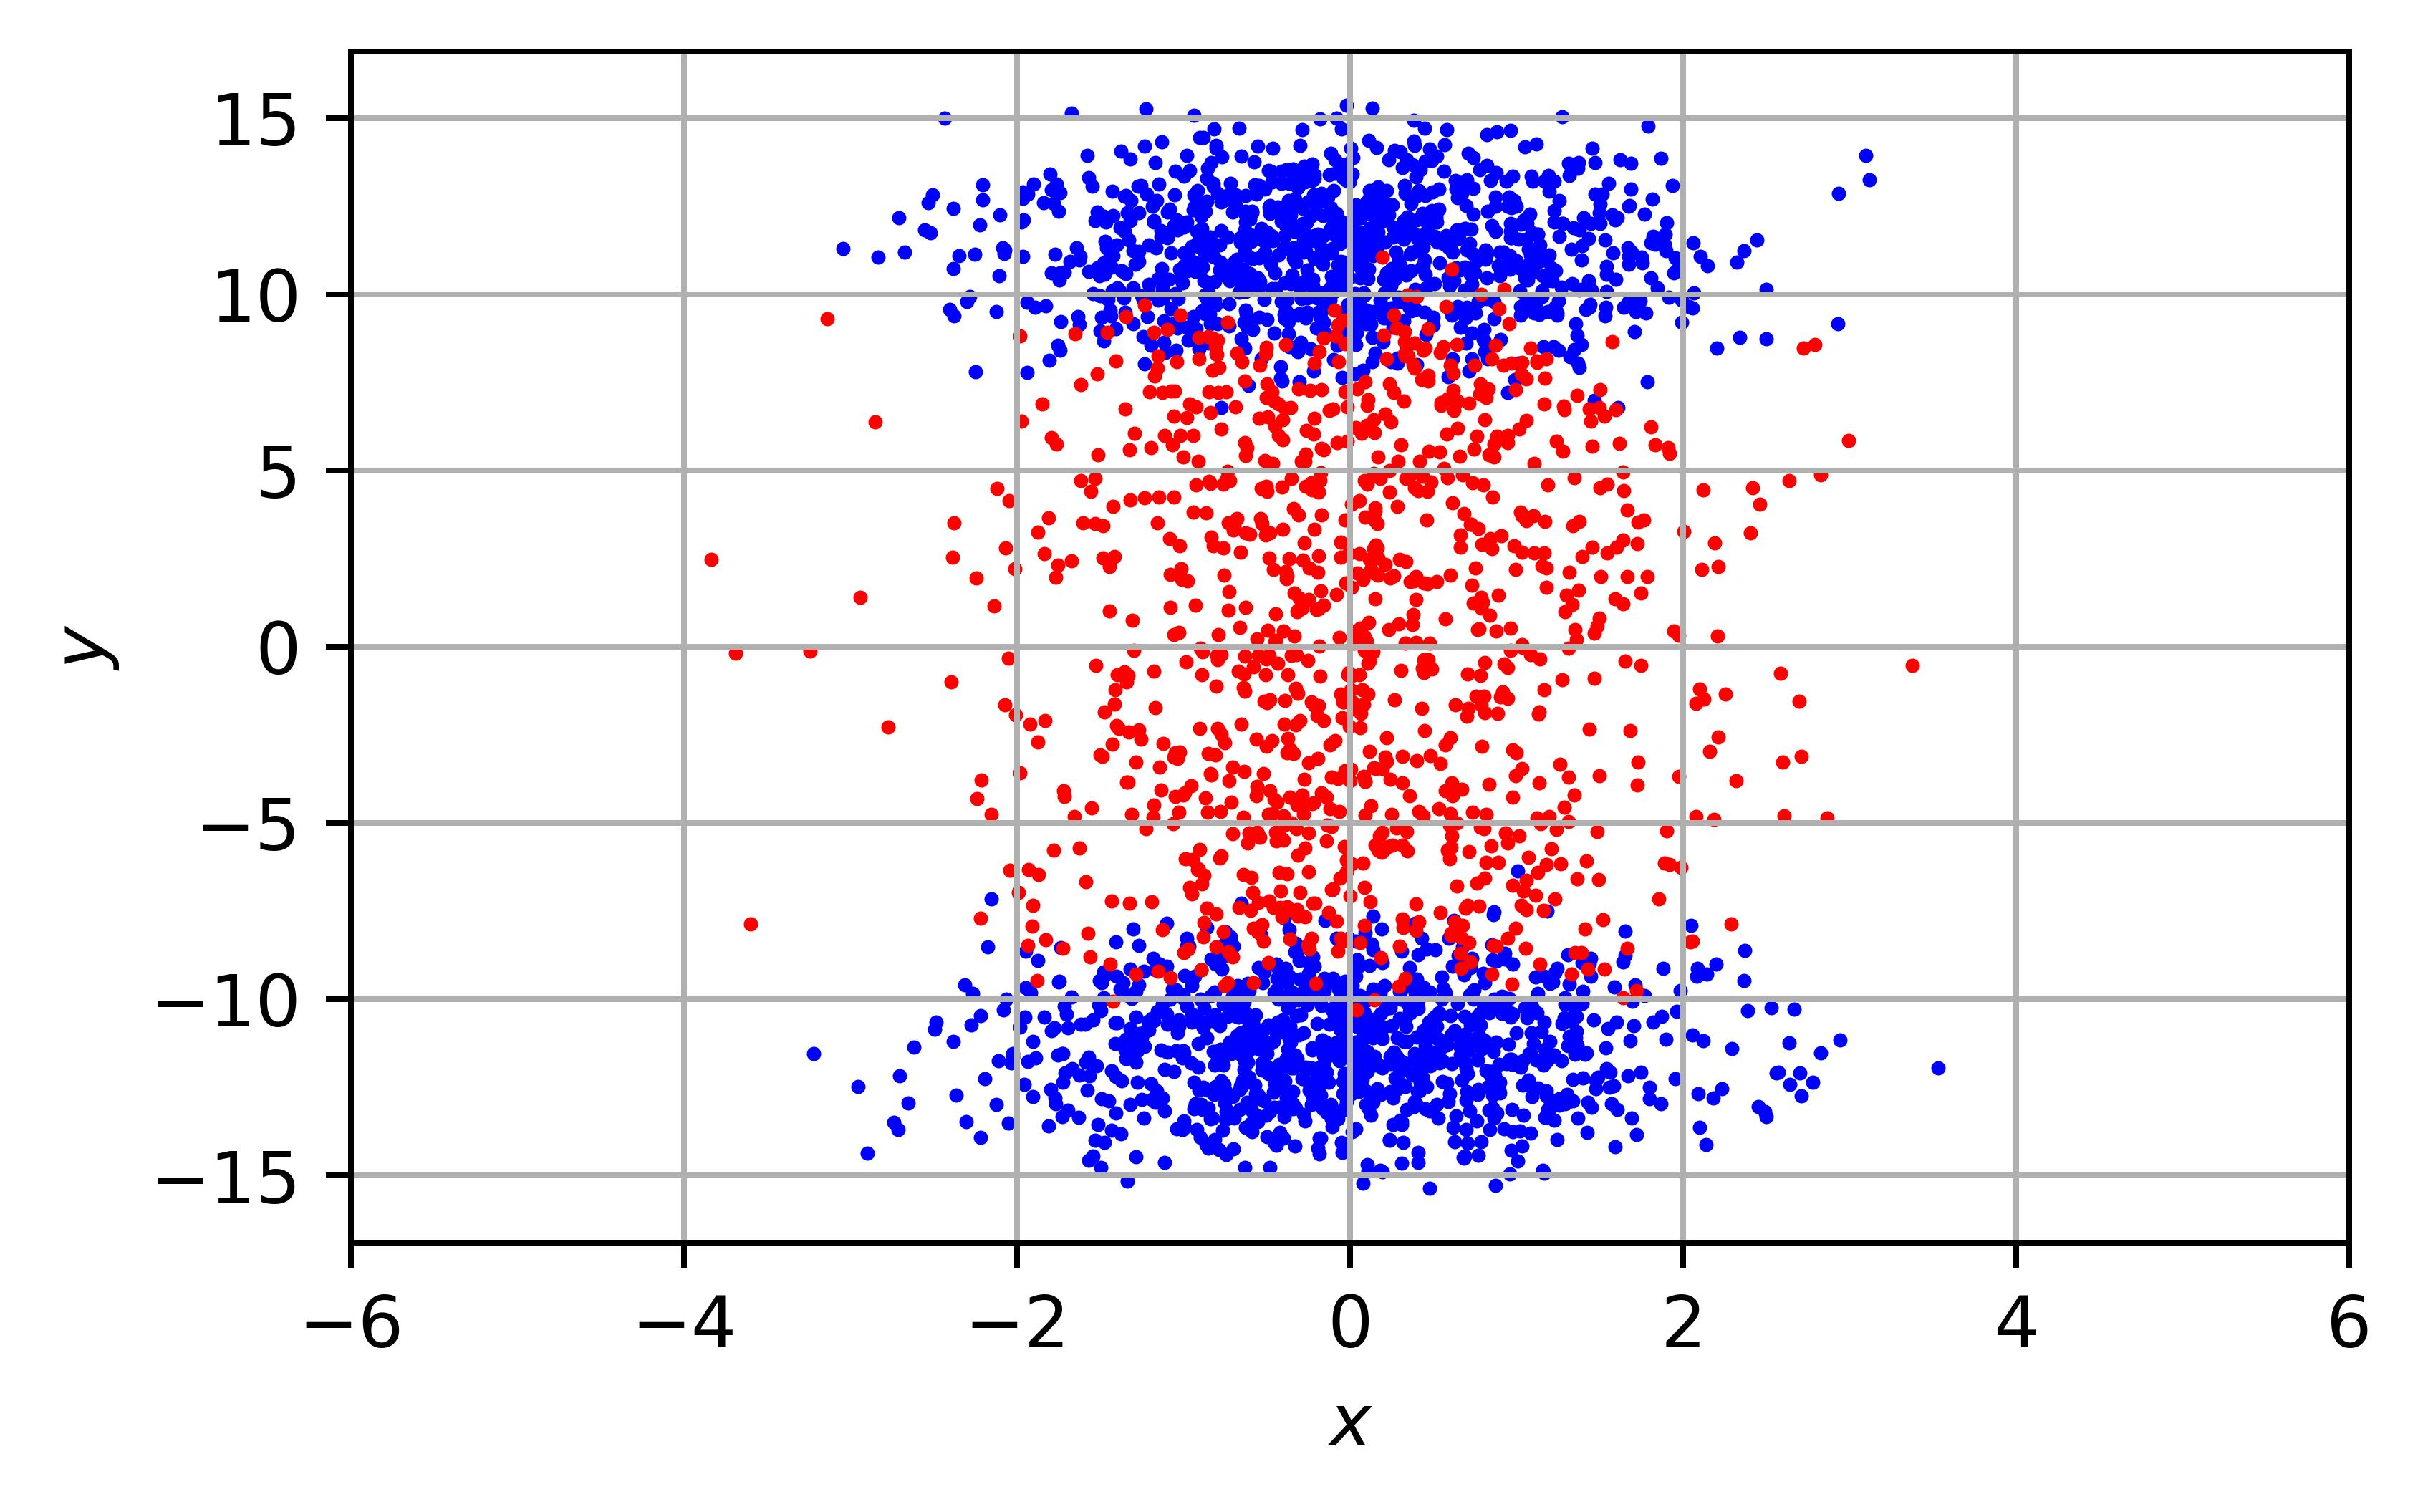
\includegraphics[width=0.4\textwidth]{./figure/Sample-Raising-1.jpg}
  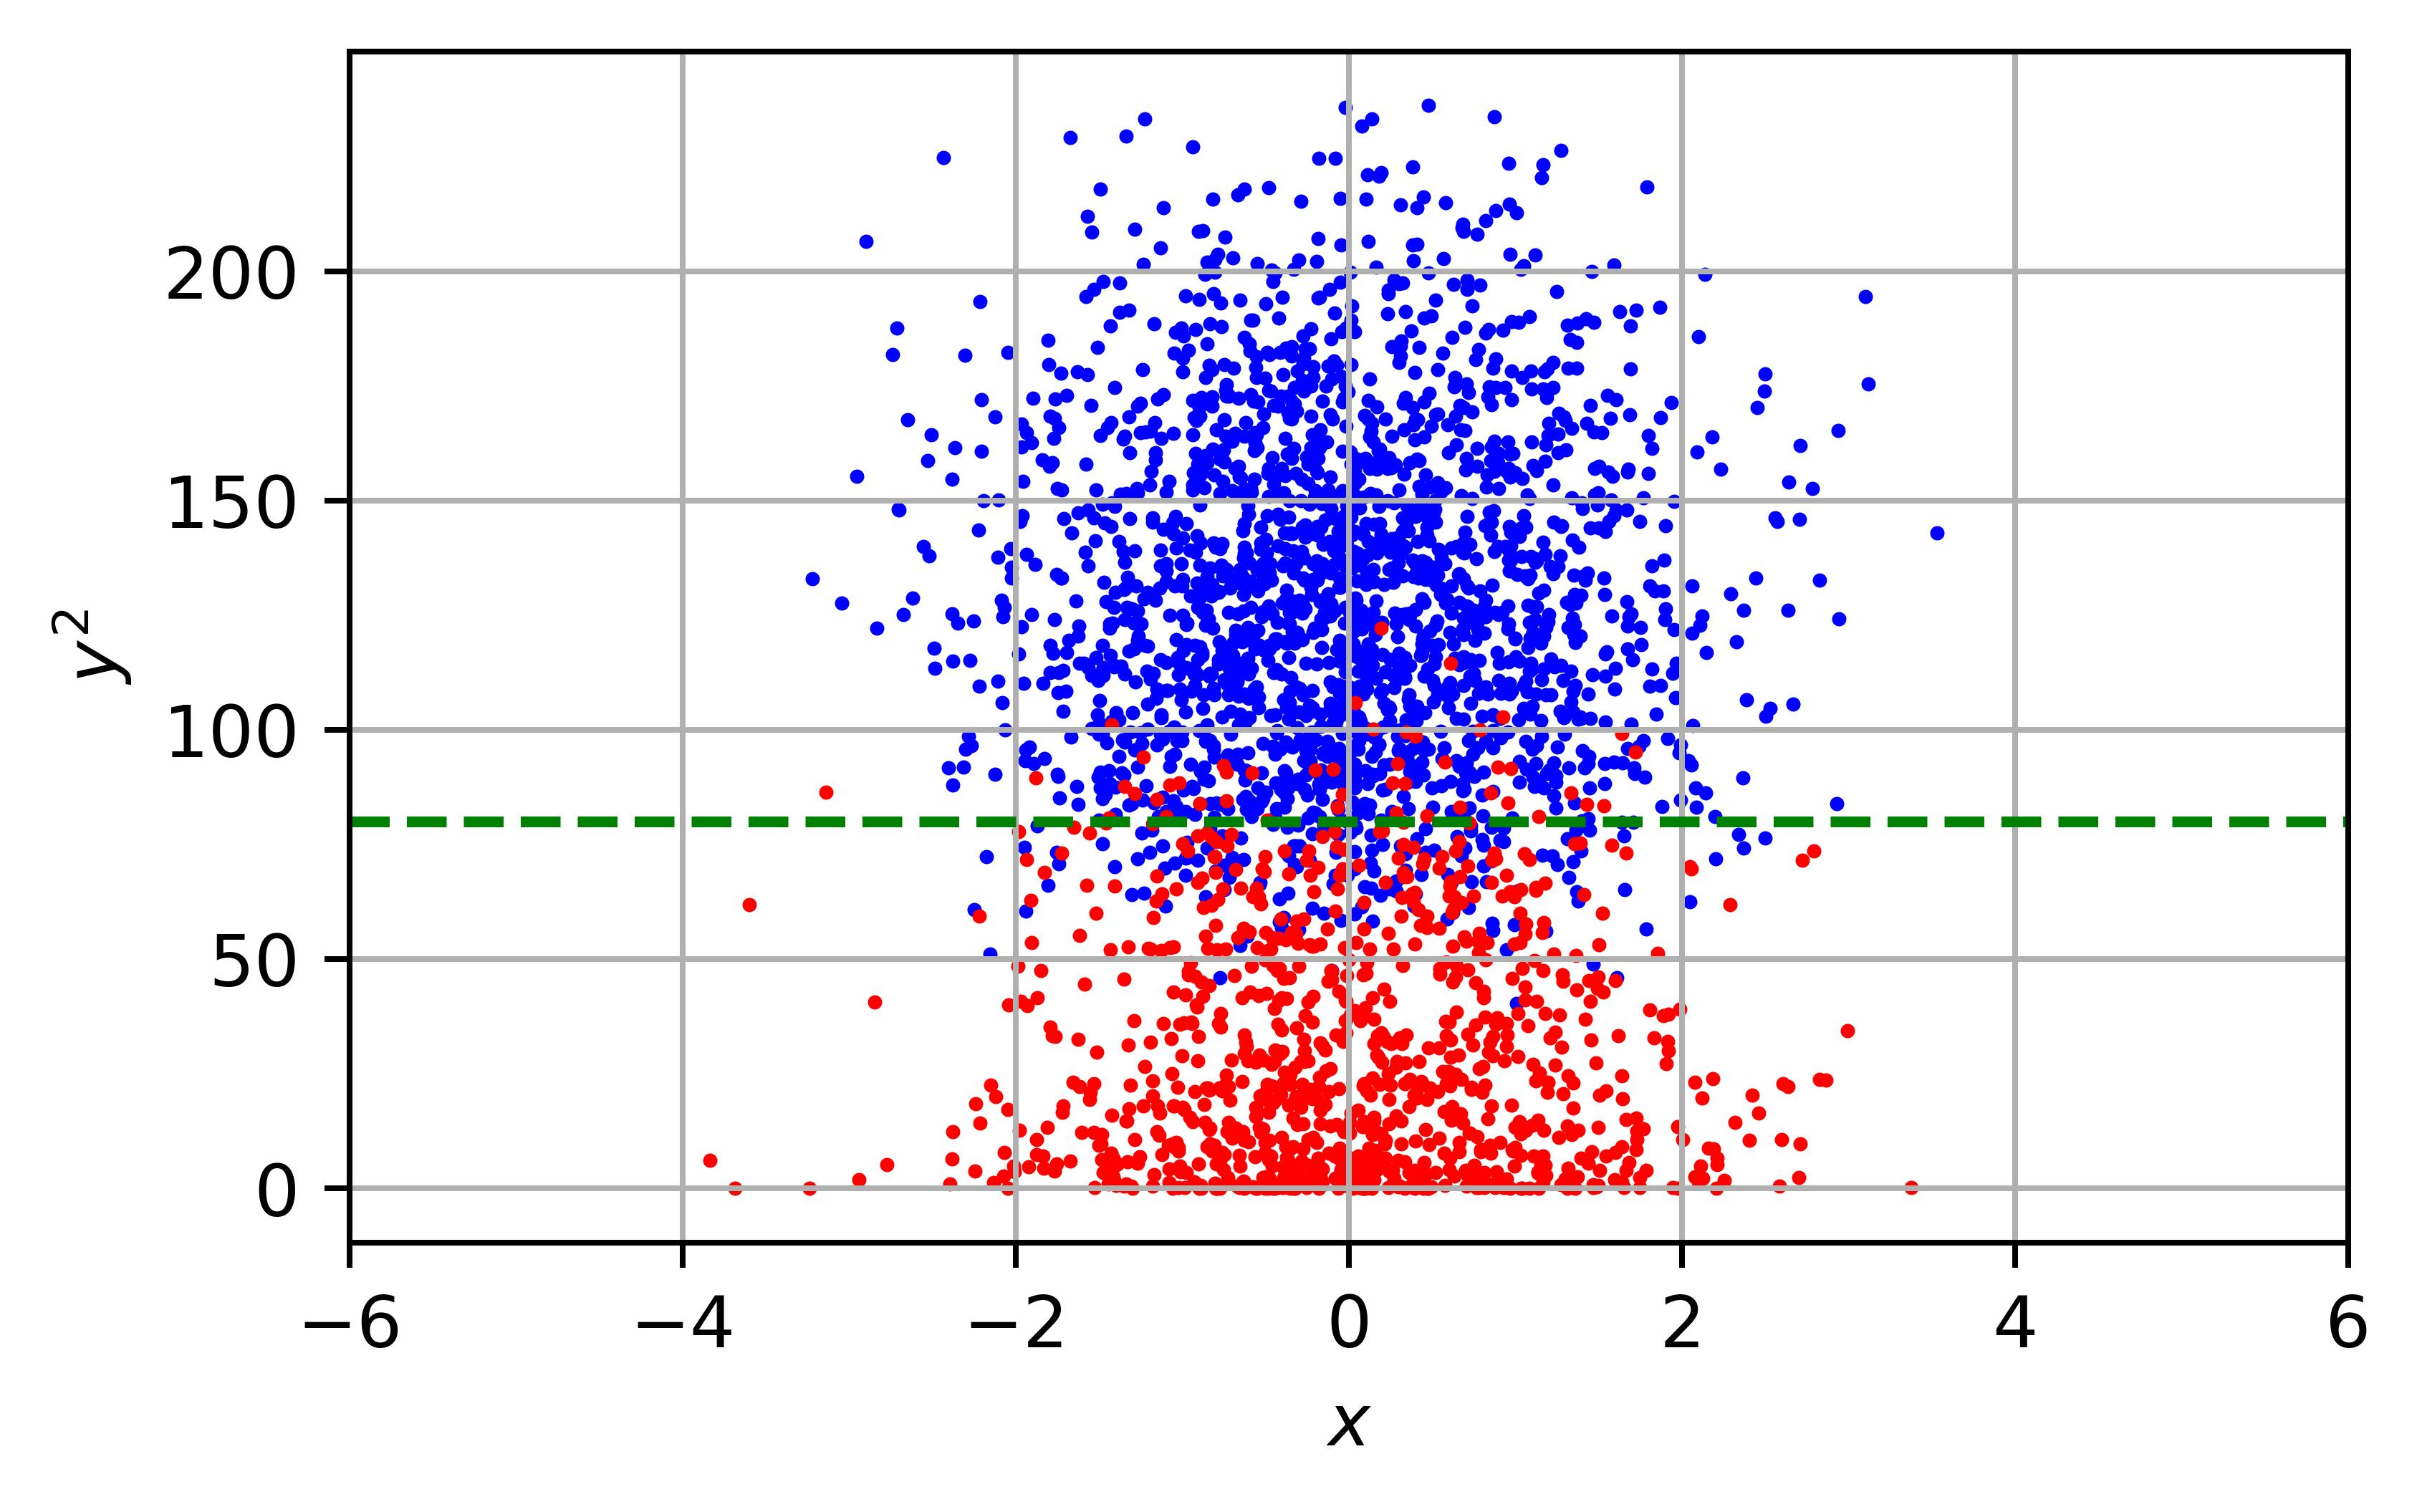
\includegraphics[width=0.4\textwidth]{./figure/Sample-Raising-2.jpg}
  \caption{Example for dimension raising. The left shows that the origin data is not linearly separable, while the right shows the data after dimension raising, where the $y_2$ is easy to be separated by a line.}
  \label{sample-raising}
\end{figure}

\section{Data Analysis Method \& Implementation}

\subsection{Logistic regression}

The logistic regression \cite{walker1967estimation} \cite{pohar2004comparison} is a widely used classification model with less prone to overfitting due to its linearty. By linearly combine the input features, the logistic regression gives a probability value ranging between $0$ and $1$ as output via

$$
  p (\mathbf{x}) = \frac{1}{1 + \exp{- \mathbf{x}^T \beta_1 - \beta_0}},
$$

\noindent with the objective function defined as the log-likelihood

$$
  l = \sum_{y_k = 1} \ln(p (\mathbf{x}_i)) + \sum_{y_k = 0} \ln(1 - p (\mathbf{x}_i)),
$$

\noindent where $\mathbf{x}_i$ are sample and the $y_i$ are corresponding label.

Then, the a gradient descent method is used for getting the optimal parameters with the gradient of the above log-likelihood

$$
  \begin{aligned}
    \frac{\partial l}{\partial \beta_0} = & \sum_{i=0}^n (y_k - p (\mathbf{x_k})),              \\
    \frac{\partial l}{\partial \beta_1} = & \sum_{i=0}^n (y_k - p (\mathbf{x_k})) \mathbf{x_k}, \\
  \end{aligned}
$$

\noindent where $n$ is the number of samples.

Further more, we used a learning rate adjusting strategy similar to Adagrad, combining with the learning rate schedule to accelerate the convergence. Specifically, the learning rate in $k$-th interaction is given by

$$
  \eta_k = \frac{\eta_0 \gamma^{\lfloor \frac{k}{m} \rfloor}}{\max(1.0, \Vert \nabla l \Vert + \epsilon)},
$$

\noindent where $\eta_0$ is the initial learning rate, $m$ is the interval of learning rate schedule and $\epsilon$ is a small value to avoid the division by zero.

We implement the above method with the Lasso and Ridge penalty by PyTorch, most of the hyperparameters are given by the user via the command, while the interval of learning rate schedule is fix to $2048$ iterations. The norm we used for adapting and terminating condition is the $l-\infty$ norm, which can also be written as $\max_{i} \vert d_i \vert$, where $d_i$ is the $i$-th entry of the gradient. Different from $l_1$ norm and $l_2$ norm, the $l-\infty$ norm doesn't involve the dimension, thus it will be more suitable for different problems due to the consistency.

\subsection{Decision tree}

The decision tree \cite{utgoff1989incremental} \cite{kotsiantis2013decision} is a supervised learning method used for classification. Based on the simple decision rules inferred from the data features, it will create a model that predict the label with piecewise constant approximation. More specifically, given the samples $s = \{(x_i, y_i)\}_{i=1}^n$ the Gini index and the Entropy is computed as

$$
  \begin{aligned}
    \text{Gini} (x, y) =    & 1 - \sum_{k=1}^m p_k^2,          \\
    \text{Entropy} (x, y) = & - \sum_{k=1}^m p_k \log_2 (p_k), \\
  \end{aligned}
$$

\noindent where $m$ is the number of classes, and $p_k$ is the proportion of class $k$. Then a threshold $t$ will be found to split the smaples into $s_1 = \{(x_i, y_i): (x_i, y_i) \in s, x_i <= t \}$ and $s_2 = \{(x_i, y_i): (x_i, y_i) \in s, x_i > t \}$ such that the information gain, i.e., the Gini index or the Entropy of $s$ minus the sum of the Gini index or the Entropy of the $s_1$ and $s_2$, will reach the maximum.

We implement the decision tree by PyTorch, with the maximal depth, minimal number of samples to split, minimal number of samples in leaf selected by user, which are the terminating conditions in creating the tree. In optimizing the threshold of splitting, the grid search method is used for accelerating, i.e., given the samples $\{x_i\}_{i=1}^n$ and the number of grid point $m + 1$, we first generate the grid point as

$$
  p_i = \min(x_i) + \frac{\max(x_i) - \min(x_i)}{m} i, i \in \{0, \dots, m\},
$$

\noindent where $p_0 = \min(x_i)$ and $p_{m} = \max(x_i)$ and the grid is uniform. Noticed that this approach is used only when the number of unique values in $x$ is larger than a given threshold, otherwise, we simply use the unique values in $x$ as well as the mid point of two adjacent smaples as the grid.

After compute the grid, we can calculate the information gain for all splitting point in one turn with the support of PyTorch tensor, which can speed up the generation by hundreds of times.

\subsection{Multilayer perceptron}

The multilayer perceptron (MLP) \cite{rosenblatt1958perceptron} \cite{rumelhart1986learning} is a basic kind of neural network which learns a function $f: \mathbb{R}^n \mapsto \mathbb{R}^m$ to approximate the input and output. Differnet from the logistic regression, the MLP includes some hidden layer with the nonlinear active function, which can help handle nonlineariy of the data, as well as the hierarchical feature extraction, i.e., it can capturing increasingly complex patterns level by level.

We implement the MLP by PyTorch with Adam optimizer \cite{kingma2014adam} , which can help train the network efficiently. The hyperparameters including size of each batch, size of hidden layer, dropout rate and number of total epoch are given by users, and during our test a large batch size is used to accelerate the training. We used LeakyReLU as activate function, as well as batch normalization and dropout for better performance and avoiding the overfitting.

\section{Solution \& Preformance}

\subsection{Task 1}

The Figure \ref{task-1-overview-flowchart} shows the workflow of task 1. During the preparing, we used the dimension raising based on the data distribution as well as the meaning of each features. Also, the correlation coefficients between label and each features are computed as other evidence for feature engineering. After the preparing, the logistic regression and decision tree are implemented and applied to the data, with different hyperparameters to show the effect of them. In the end, the macro f1 score is used to evaluate the model. In the meanwhile, the time and memory cost is also recorded for analysis.

\begin{figure}[H]
  \centering
  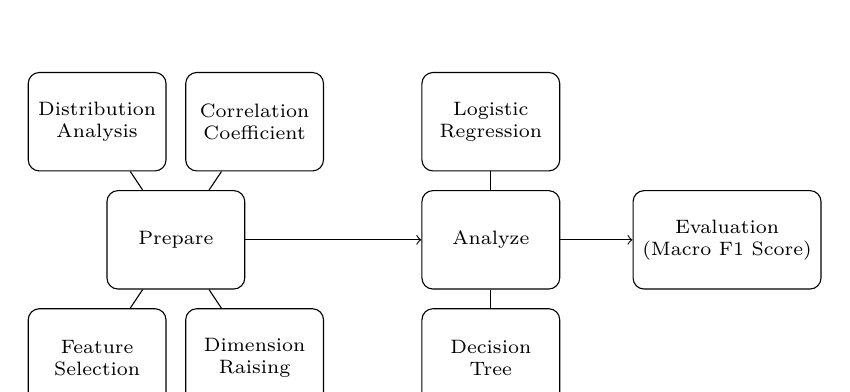
\begin{tikzpicture}[minimum width=1.75cm, minimum height=1.25cm, font=\scriptsize]
    \node[draw, align=center, rounded corners]  (P)   at ( 0,  0.0)    {Prepare};
    \node[draw, align=center, rounded corners]  (D)   at (-1,  1.5)    {Distribution \\ Analysis};
    \node[draw, align=center, rounded corners]  (C)   at ( 1,  1.5)    {Correlation \\ Coefficient};
    \node[draw, align=center, rounded corners]  (F)   at (-1, -1.5)    {Feature \\ Selection};
    \node[draw, align=center, rounded corners]  (R)   at ( 1, -1.5)    {Dimension \\ Raising};

    \node[draw, align=center, rounded corners]  (M)   at ( 4,  0.0)    {Analyze};
    \node[draw, align=center, rounded corners]  (LR)  at ( 4,  1.5)    {Logistic \\ Regression};
    \node[draw, align=center, rounded corners]  (DT)  at ( 4, -1.5)    {Decision \\ Tree};

    \node[draw, align=center, rounded corners]  (E)   at ( 7,  0.0)    {Evaluation \\ (Macro F1 Score)};

    \draw[->] (P) -- (M);

    \draw[-]  (P) -- (D);
    \draw[-]  (P) -- (C);
    \draw[-]  (P) -- (F);
    \draw[-]  (P) -- (R);

    \draw[-]  (M) -- (LR);
    \draw[-]  (M) -- (DT);

    \draw[->] (M) -- (E);
  \end{tikzpicture}
  \caption{Overview flowchart for task 1.}
  \label{task-1-overview-flowchart}
\end{figure}

The Figure \ref{task-1-data-distribution} is the parallel coordinate plot of the data. And the Figure \ref{task-1-correlation-coefficient} shows the correlation coefficient between the label and each features.

From These figures, we can easly see that some features (e.g. AptitudeTestScore and HSC\_Marks) are linear separatable with the absolute value of every correlation coefficients more than $0.4$, implies that these features are highly highly relevant to the label, and can be directly used in the predicting model. In addition, all the correlation coefficients are all higher then $0.2$, which implies the linear model can get a good preformance on this dataset.

Another property of the data is that there is no anonymity features and all features has its meaning. Therefore we can manually create the new features based on their meanings. For example, the Internships, Projects and Workshops/Certifications are all practical experiences, thus we create a new features from them, which shows that whether the student have ever participate in a practice; the AptitudeTestScore and SoftSkillsRating are all about the potential ability, which can also be combined; there is chronological relationship betwenn SSC\_Marks and HSC\_Marks, thus its difference can be used to measure the effort of student in this period; and so on so forth for other features.

\begin{figure}[H]
  \centering
  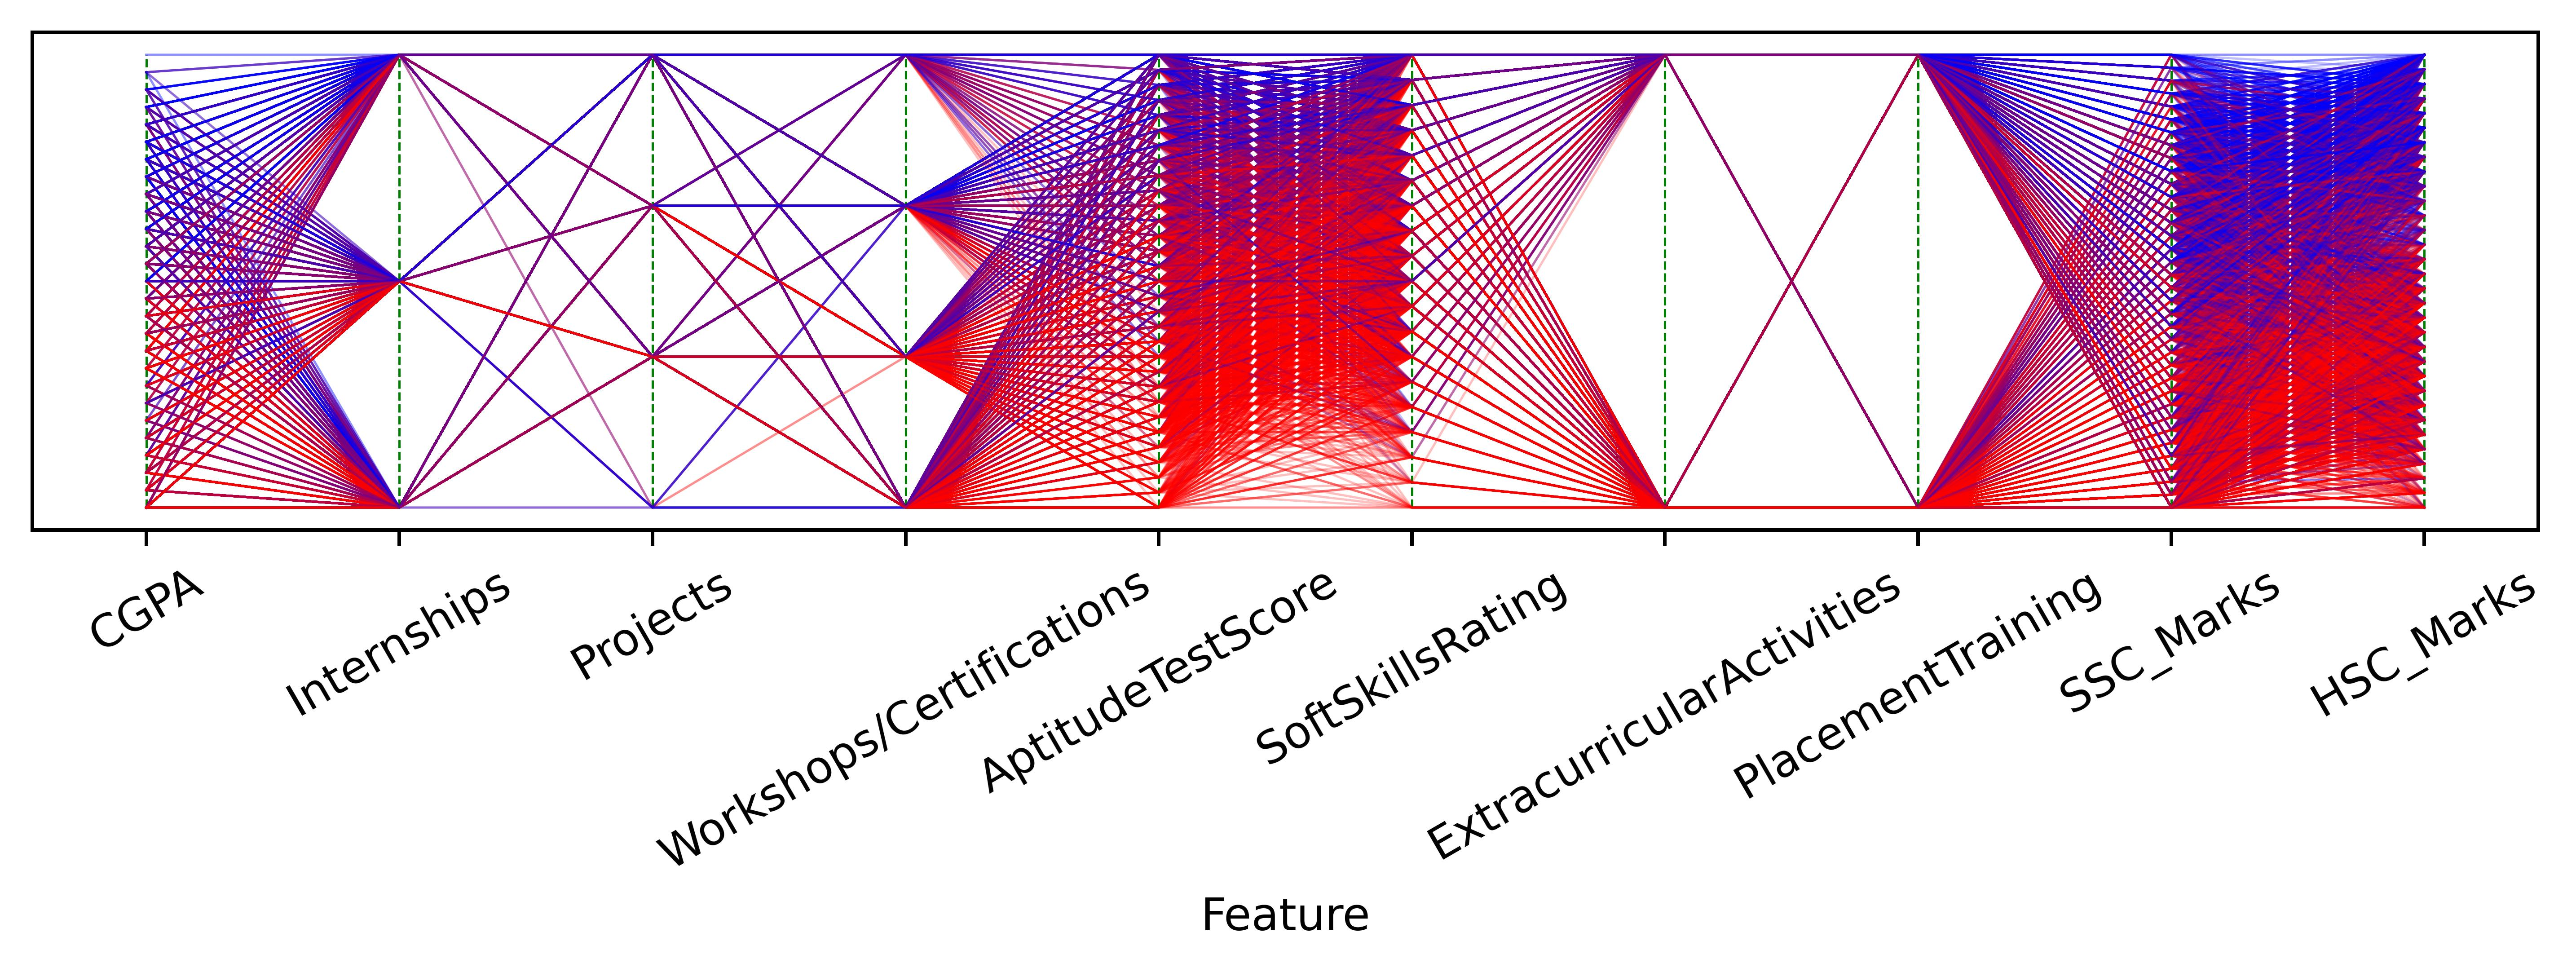
\includegraphics[width=\textwidth]{../code/Task1/Analysis/PC.jpg}
  \caption{The parallel coordinate plot for each features.}
  \label{task-1-data-distribution}
\end{figure}

\begin{figure}[H]
  \centering
  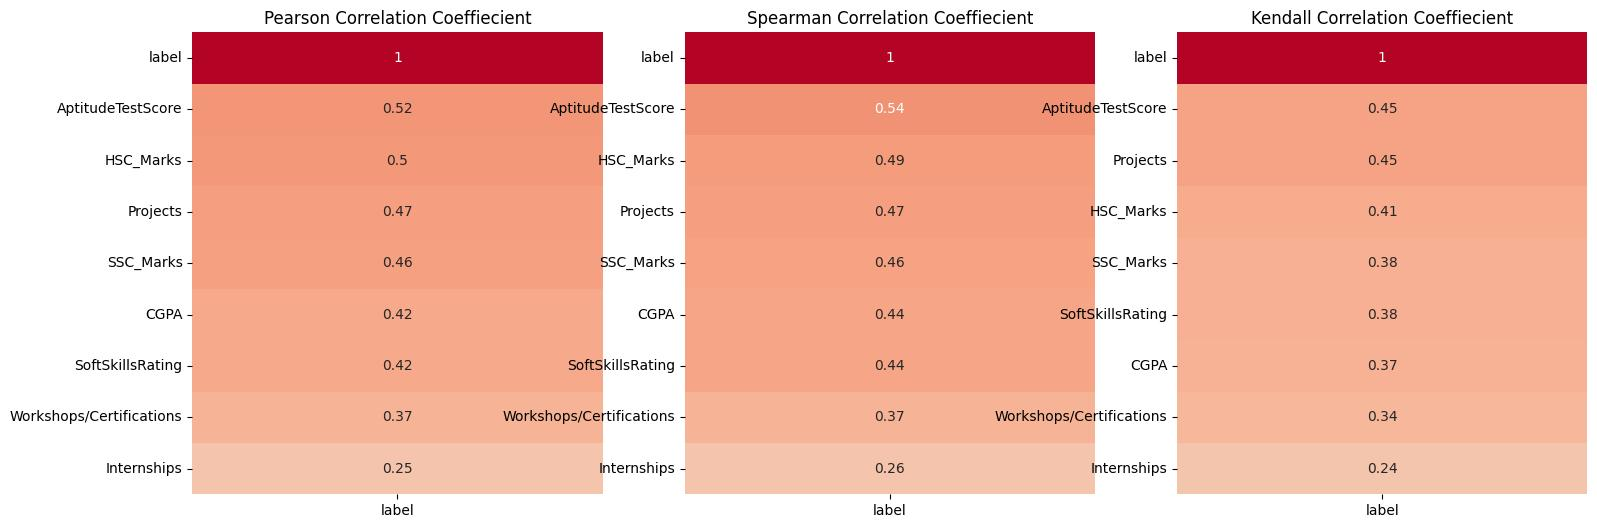
\includegraphics[width=\textwidth]{../code/Task1/Analysis/corrcoef.jpg} \\
  \caption{Correlation coefficient for each features.}
  \label{task-1-correlation-coefficient}
\end{figure}

After the preparing, the logistic regression and decision tree is applied to the data. The Table \ref{task-1-result-1} and Table \ref{task-1-result-2} shows the results of logistic regression and decision tree with different hyperparameters. Each test includes $5$ times cross validation ($80\%$ for training set, $20\%$ for training set) and $1$ times that using all data as training set. And the macro f1 score, time and memory cost are recorded.

The result shows that the logistic regression can reach the f1 score about $0.79$ while the decision tree can only get the $0.75$. This might be caused by the overfitting of the decision tree, since there is a large gap between the f1 score on the testing data and training data. Further more, in this task, the dimension raising doesn't give a better preformance, which implies that the relationships between labels and origin data might be linear. However, the lasso and ridge penalty can lead to a better f1 score, which means that some features are useless and can influence the optimizing.

\begin{table}[H]
  \centering
  \begin{tabular}{|c|c|c|c|}
    \hline
    Penalty & \makecell{Dimension                                \\ Raising \\ (Degree)} & \makecell{F1 Score \\ (Test/Train)} & \makecell{Time/Mem \\ (s/MB)} \\
    \hline
    None    & None                & $0.7909/0.7933$ & $1.55/735$ \\
    \hline
    None    & $2$                 & $0.7905/0.7936$ & $1.41/730$ \\
    \hline
    None    & $3$                 & $0.7909/0.7936$ & $1.28/741$ \\
    \hline
    Lasso   & None                & $0.7912/0.7927$ & $1.66/736$ \\
    \hline
    Ridge   & None                & $0.7915/0.7928$ & $1.65/735$ \\
    \hline
  \end{tabular}
  \caption{Preformance for logistic regression. We tested each option with $5$ times cross validation ($80\%$ for training set, $20\%$ for training set) and $1$ times that using all data as training set. The f1 scores showed in the table is the average f1 score for cross validation and using all data as training set (in this case, we just tested the model on training data) and using all data as training set (in this case, we just tested the model on training data), the time is the total time for $6$ run, and the memory usage is tested using all the data as training set.}
  \label{task-1-result-1}
\end{table}

\begin{table}[H]
  \centering
  \begin{tabular}{|c|c|c|c|c|}
    \hline
    Max Depth & \makecell{Number of                                          \\ Threshold} & Criterion & \makecell{F1 Score \\ (Test/Train)} & \makecell{Time/Mem \\ (s/MB)}               \\
    \hline
    $10$      & $64$                & gini    & $0.7502/0.8677$ & $17.5/497$ \\
    \hline
    $10$      & $128$               & gini    & $0.7485/0.8698$ & $16.4/498$ \\
    \hline
    $12$      & $64$                & gini    & $0.7266/0.9089$ & $25.2/497$ \\
    \hline
    $10$      & $64$                & entropy & $0.7428/0.8500$ & $16.4/501$ \\
    \hline
  \end{tabular}
  \caption{Preformance for decision tree. We tested each option with $5$ times cross validation ($80\%$ for training set, $20\%$ for training set) and $1$ times that using all data as training set. The f1 scores showed in the table is the average f1 score for cross validation and using all data as training set (in this case, we just tested the model on training data) and using all data as training set (in this case, we just tested the model on training data), the time is the total time for $6$ run, and the memory usage is tested using all the data as training set.}
  \label{task-1-result-2}
\end{table}

\subsection{Task 2}

The Figure \ref{task-2-overview-flowchart} shows the workflow of task 2. During the preparing, we focus the missing  value problems, and the distribution of each features as well as the correlation coefficients as the auxiliary. The $k$ nearest neighbor imputer is applied to the data for filling the missing values, which fill in the values with existing data. After the preparing, the decision tree and MLP is implemented and applied to the data, with different hyperparameters to show the effect of them. The logistic regression is not considered in this task due to the highly nonlinearity. In the end, the macro f1 score is used to evaluate the model. In the meanwhile, the time and memory cost is also recorded for analysis.

\begin{figure}[H]
  \centering
  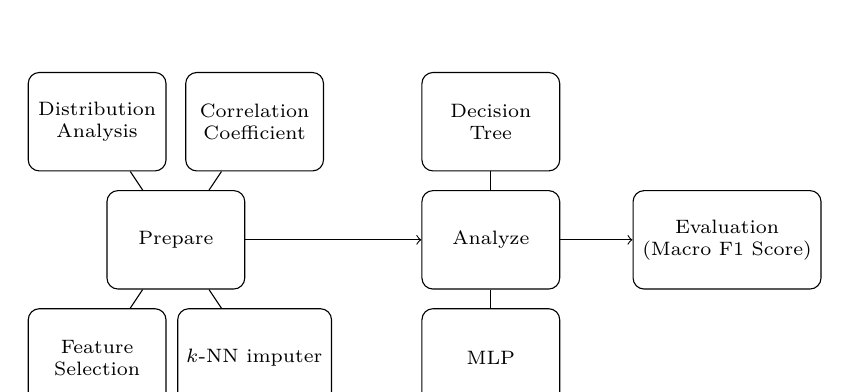
\begin{tikzpicture}[minimum width=1.75cm, minimum height=1.25cm, font=\scriptsize]
    \node[draw, align=center, rounded corners]  (P)   at ( 0,  0.0)    {Prepare};
    \node[draw, align=center, rounded corners]  (D)   at (-1,  1.5)    {Distribution \\ Analysis};
    \node[draw, align=center, rounded corners]  (C)   at ( 1,  1.5)    {Correlation \\ Coefficient};
    \node[draw, align=center, rounded corners]  (F)   at (-1, -1.5)    {Feature \\ Selection};
    \node[draw, align=center, rounded corners]  (KNN) at ( 1, -1.5)    {$k$-NN imputer};

    \node[draw, align=center, rounded corners]  (M)   at ( 4,  0.0)    {Analyze};
    \node[draw, align=center, rounded corners]  (DT)  at ( 4,  1.5)    {Decision \\ Tree};
    \node[draw, align=center, rounded corners]  (MLP) at ( 4, -1.5)    {MLP};

    \node[draw, align=center, rounded corners]  (E)   at ( 7,  0.0)    {Evaluation \\ (Macro F1 Score)};

    \draw[->] (P) -- (M);

    \draw[-]  (P) -- (D);
    \draw[-]  (P) -- (C);
    \draw[-]  (P) -- (F);
    \draw[-]  (P) -- (KNN);

    \draw[-]  (M) -- (DT);
    \draw[-]  (M) -- (MLP);

    \draw[->] (M) -- (E);
  \end{tikzpicture}
  \caption{Overview flowchart for task 2.}
  \label{task-2-overview-flowchart}
\end{figure}

The Figure \ref{task-2-missing-value} shows the number and proportion of missing values for each feature in training data, the missing values occur in few features. The features named X51, Y51, Z51 includes most missing values with the number $6634$ out of $40000$, about $16.6\%$. And the others includes no missing values or only few missing values less than $5\%$. For features with few missing values, such as X31, X41, we used the $k$ nearest neighbor imputer with the number of neighbors as the default $5$. And for the X51, Y51, Z51, the number of missing values is much larger, thus we tried two approaches: either use the $k$ nearest neighbor imputer to fill in the values, or simply drop it in the feature selection step.

\begin{table}[H]
  \centering
  \begin{tabular}{|c|c|c|c|c|c|}
    \hline
    Feature & \makecell{Number                                               \\ (Proportion)                               \\ Of Miss Value} & Feature & \makecell{Number \\ (Proportion) \\ Of Miss Value} & Feature & \makecell{Number \\ (Proportion) \\ Of Miss Value} \\
    \hline
    X01     & $0 (0.0\%)$      & Y01 & $0 (0.0\%)$    & Z01 & $0 (0.0\%)$    \\
    \hline
    X11     & $0 (0.0\%)$      & Y11 & $0 (0.0\%)$    & Z11 & $0 (0.0\%)$    \\
    \hline
    X21     & $0 (0.0\%)$      & Y21 & $0 (0.0\%)$    & Z21 & $0 (0.0\%)$    \\
    \hline
    X31     & $355 (0.9\%)$    & Y31 & $355 (0.9\%)$  & Z31 & $355 (0.9\%)$  \\
    \hline
    X41     & $1604 (4.0\%)$   & Y41 & $1604 (4.0\%)$ & Z41 & $1604 (4.0\%)$ \\
    \hline
    X51     & $6634 (16.6\%)$  & Y51 & $6634 (0.0\%)$ & Z51 & $6634 (0.0\%)$ \\
    \hline
  \end{tabular}
  \caption{The number and proportion of missing values for each feature in training data.}
  \label{task-2-missing-value}
\end{table}

The Figure \ref{task-2-data-distribution-feature} shows the distribution of each feature, where the top and bottom $5\%$ points are considered as outliers, which are not shown in the figure, but still used in training model. And the vertical lines shows the position of first, second and third quartiles. And the Figure \ref{task-2-correlation-coefficient} shows the correlation coefficient between each label and each features.

For each features, it is hard to separated the data with different labels, but there are still some useful properties. For class 1 (red), the data distribution of each features are quite different. For example, for features Y01, T21 and Y41, the red part occurs mostly in the middle of the range, while for features Z31, Z41, it appears at the left side. And for class 2 (blue), the data always occurs on the right side. From the above we can easily build a model to classify the class 1 and 2, and so on so forth for the other classes.

The correlation coefficient also shows that some features are useful. For example, the feature Z41 reaches $0.4$ of correlation with class 2, while it only get less than $0.1$ of correlation for classes 3, 4 and 5. These results implies that there exists some features that only related to only one or two classed, which can be useful in classification.

\begin{figure}[H]
  \centering
  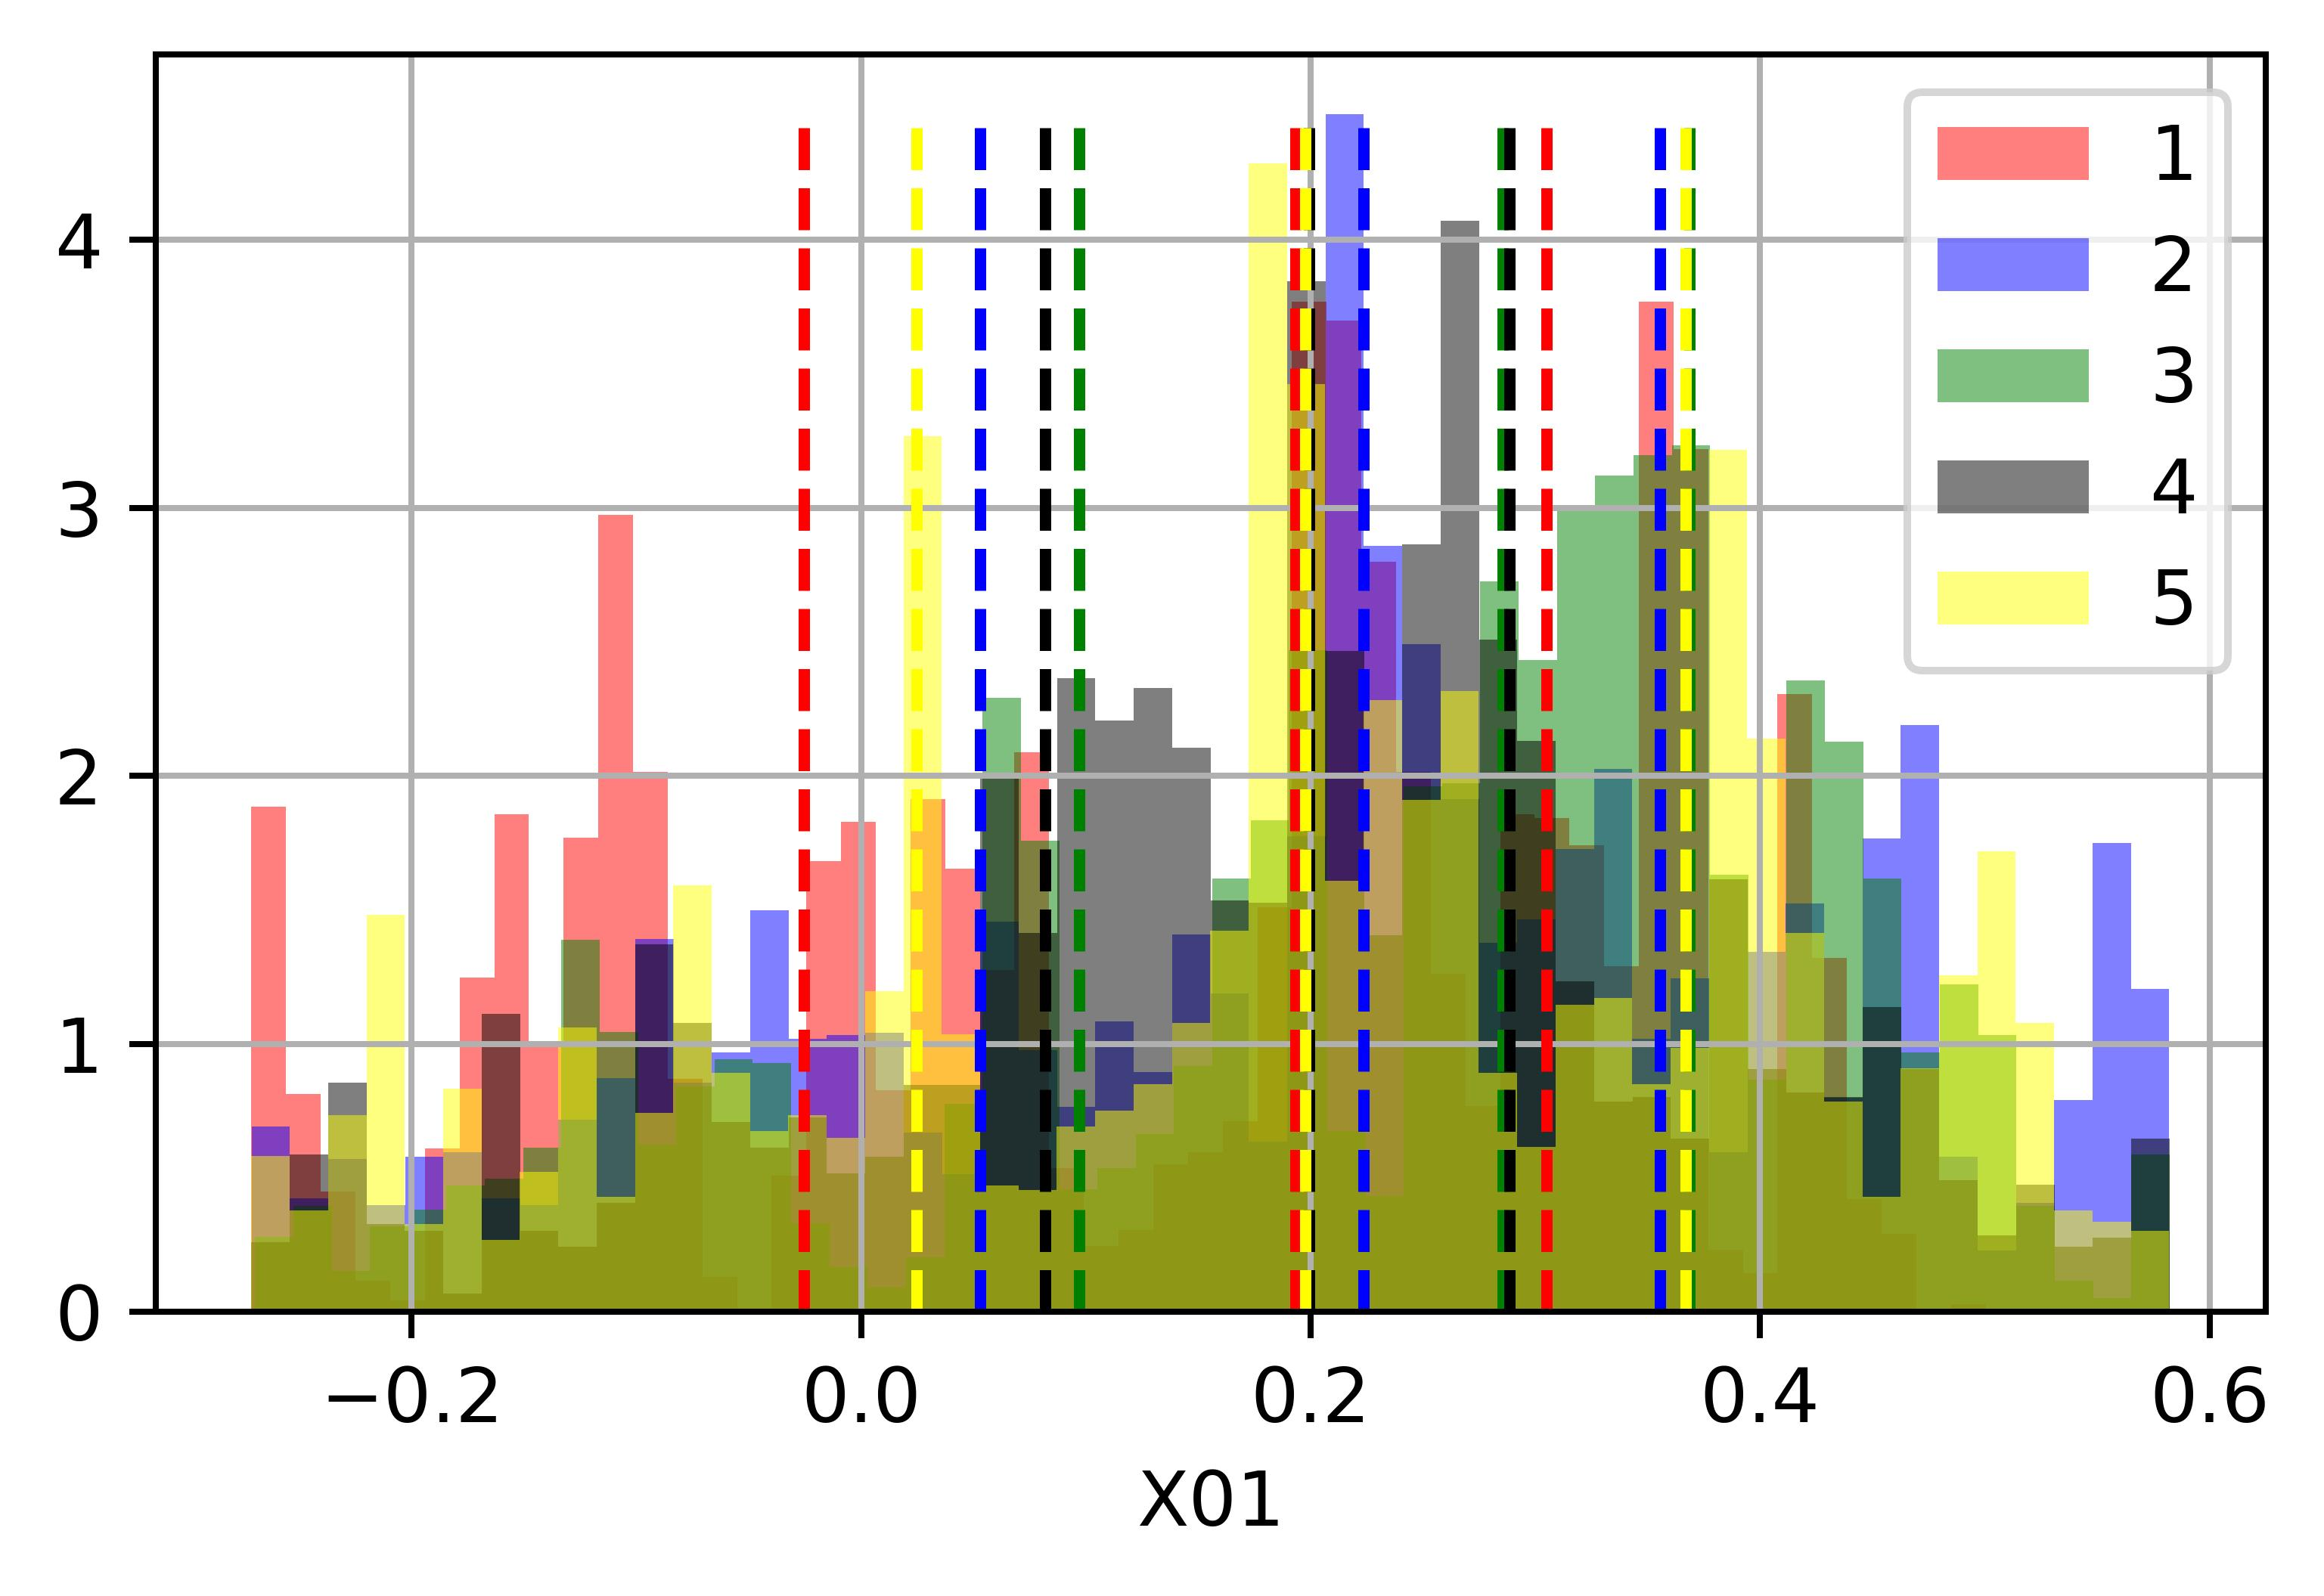
\includegraphics[width=0.18\textwidth]{../code/Task2/Analysis/Hist-X01}
  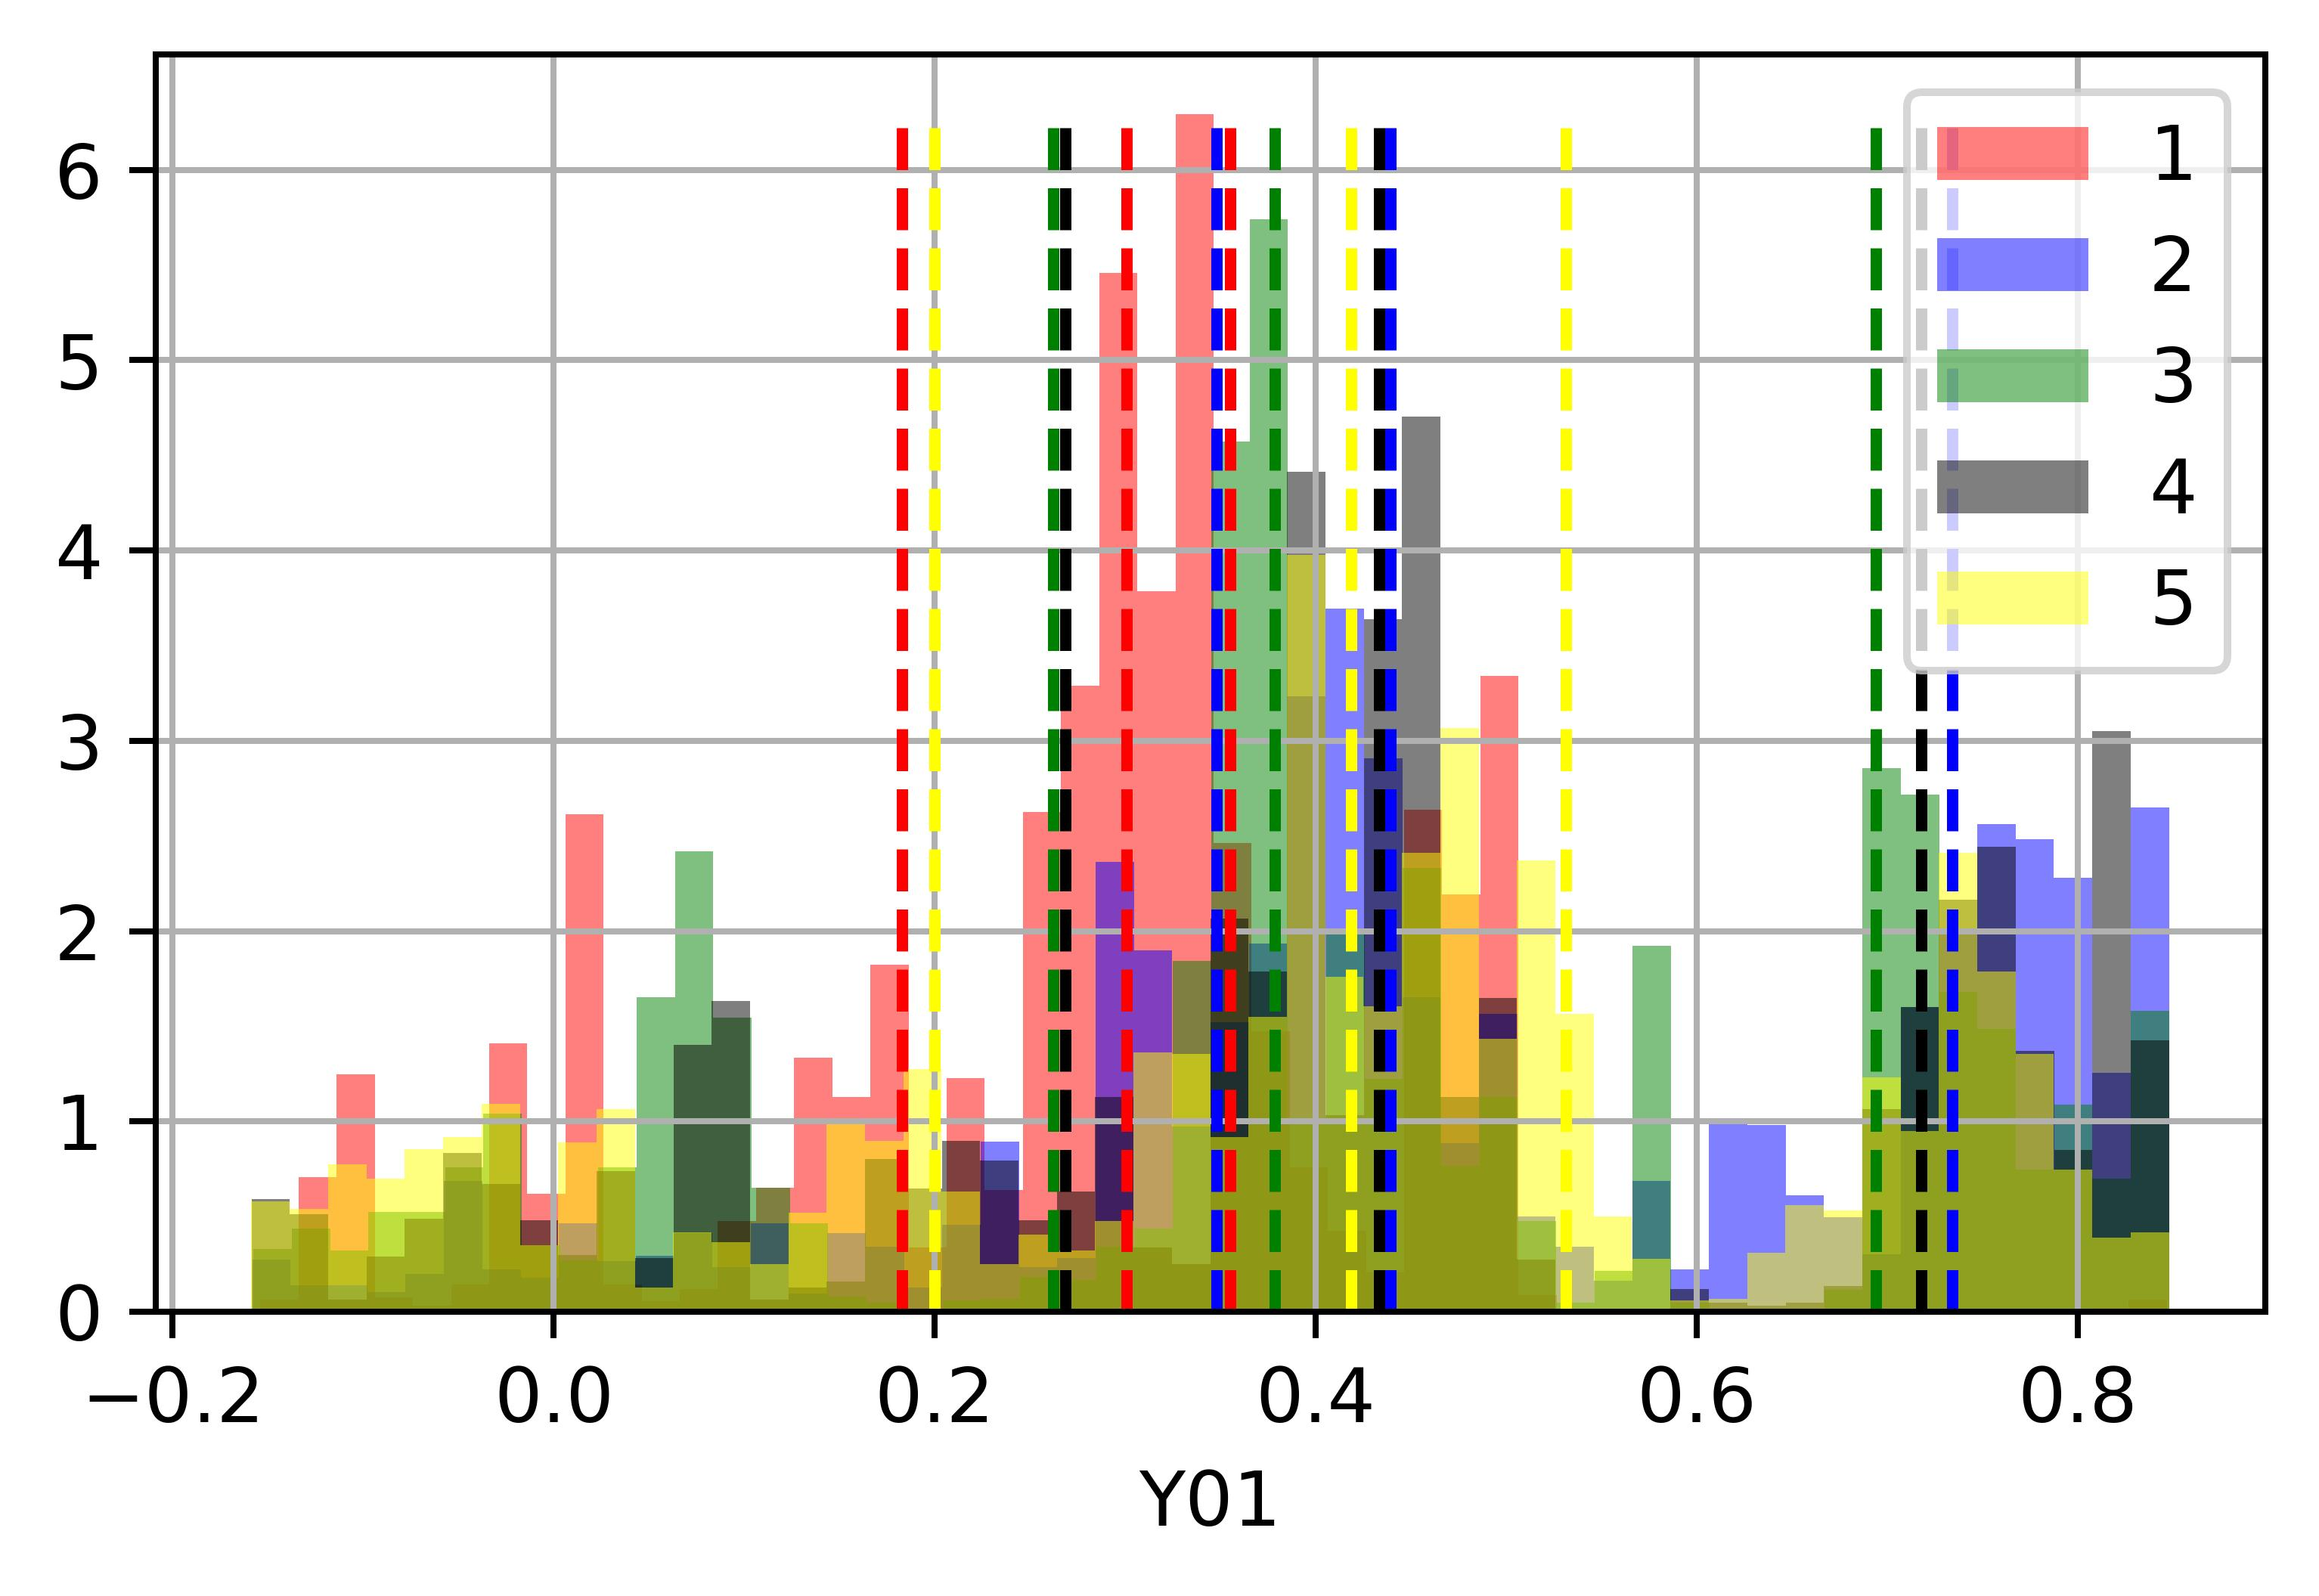
\includegraphics[width=0.18\textwidth]{../code/Task2/Analysis/Hist-Y01}
  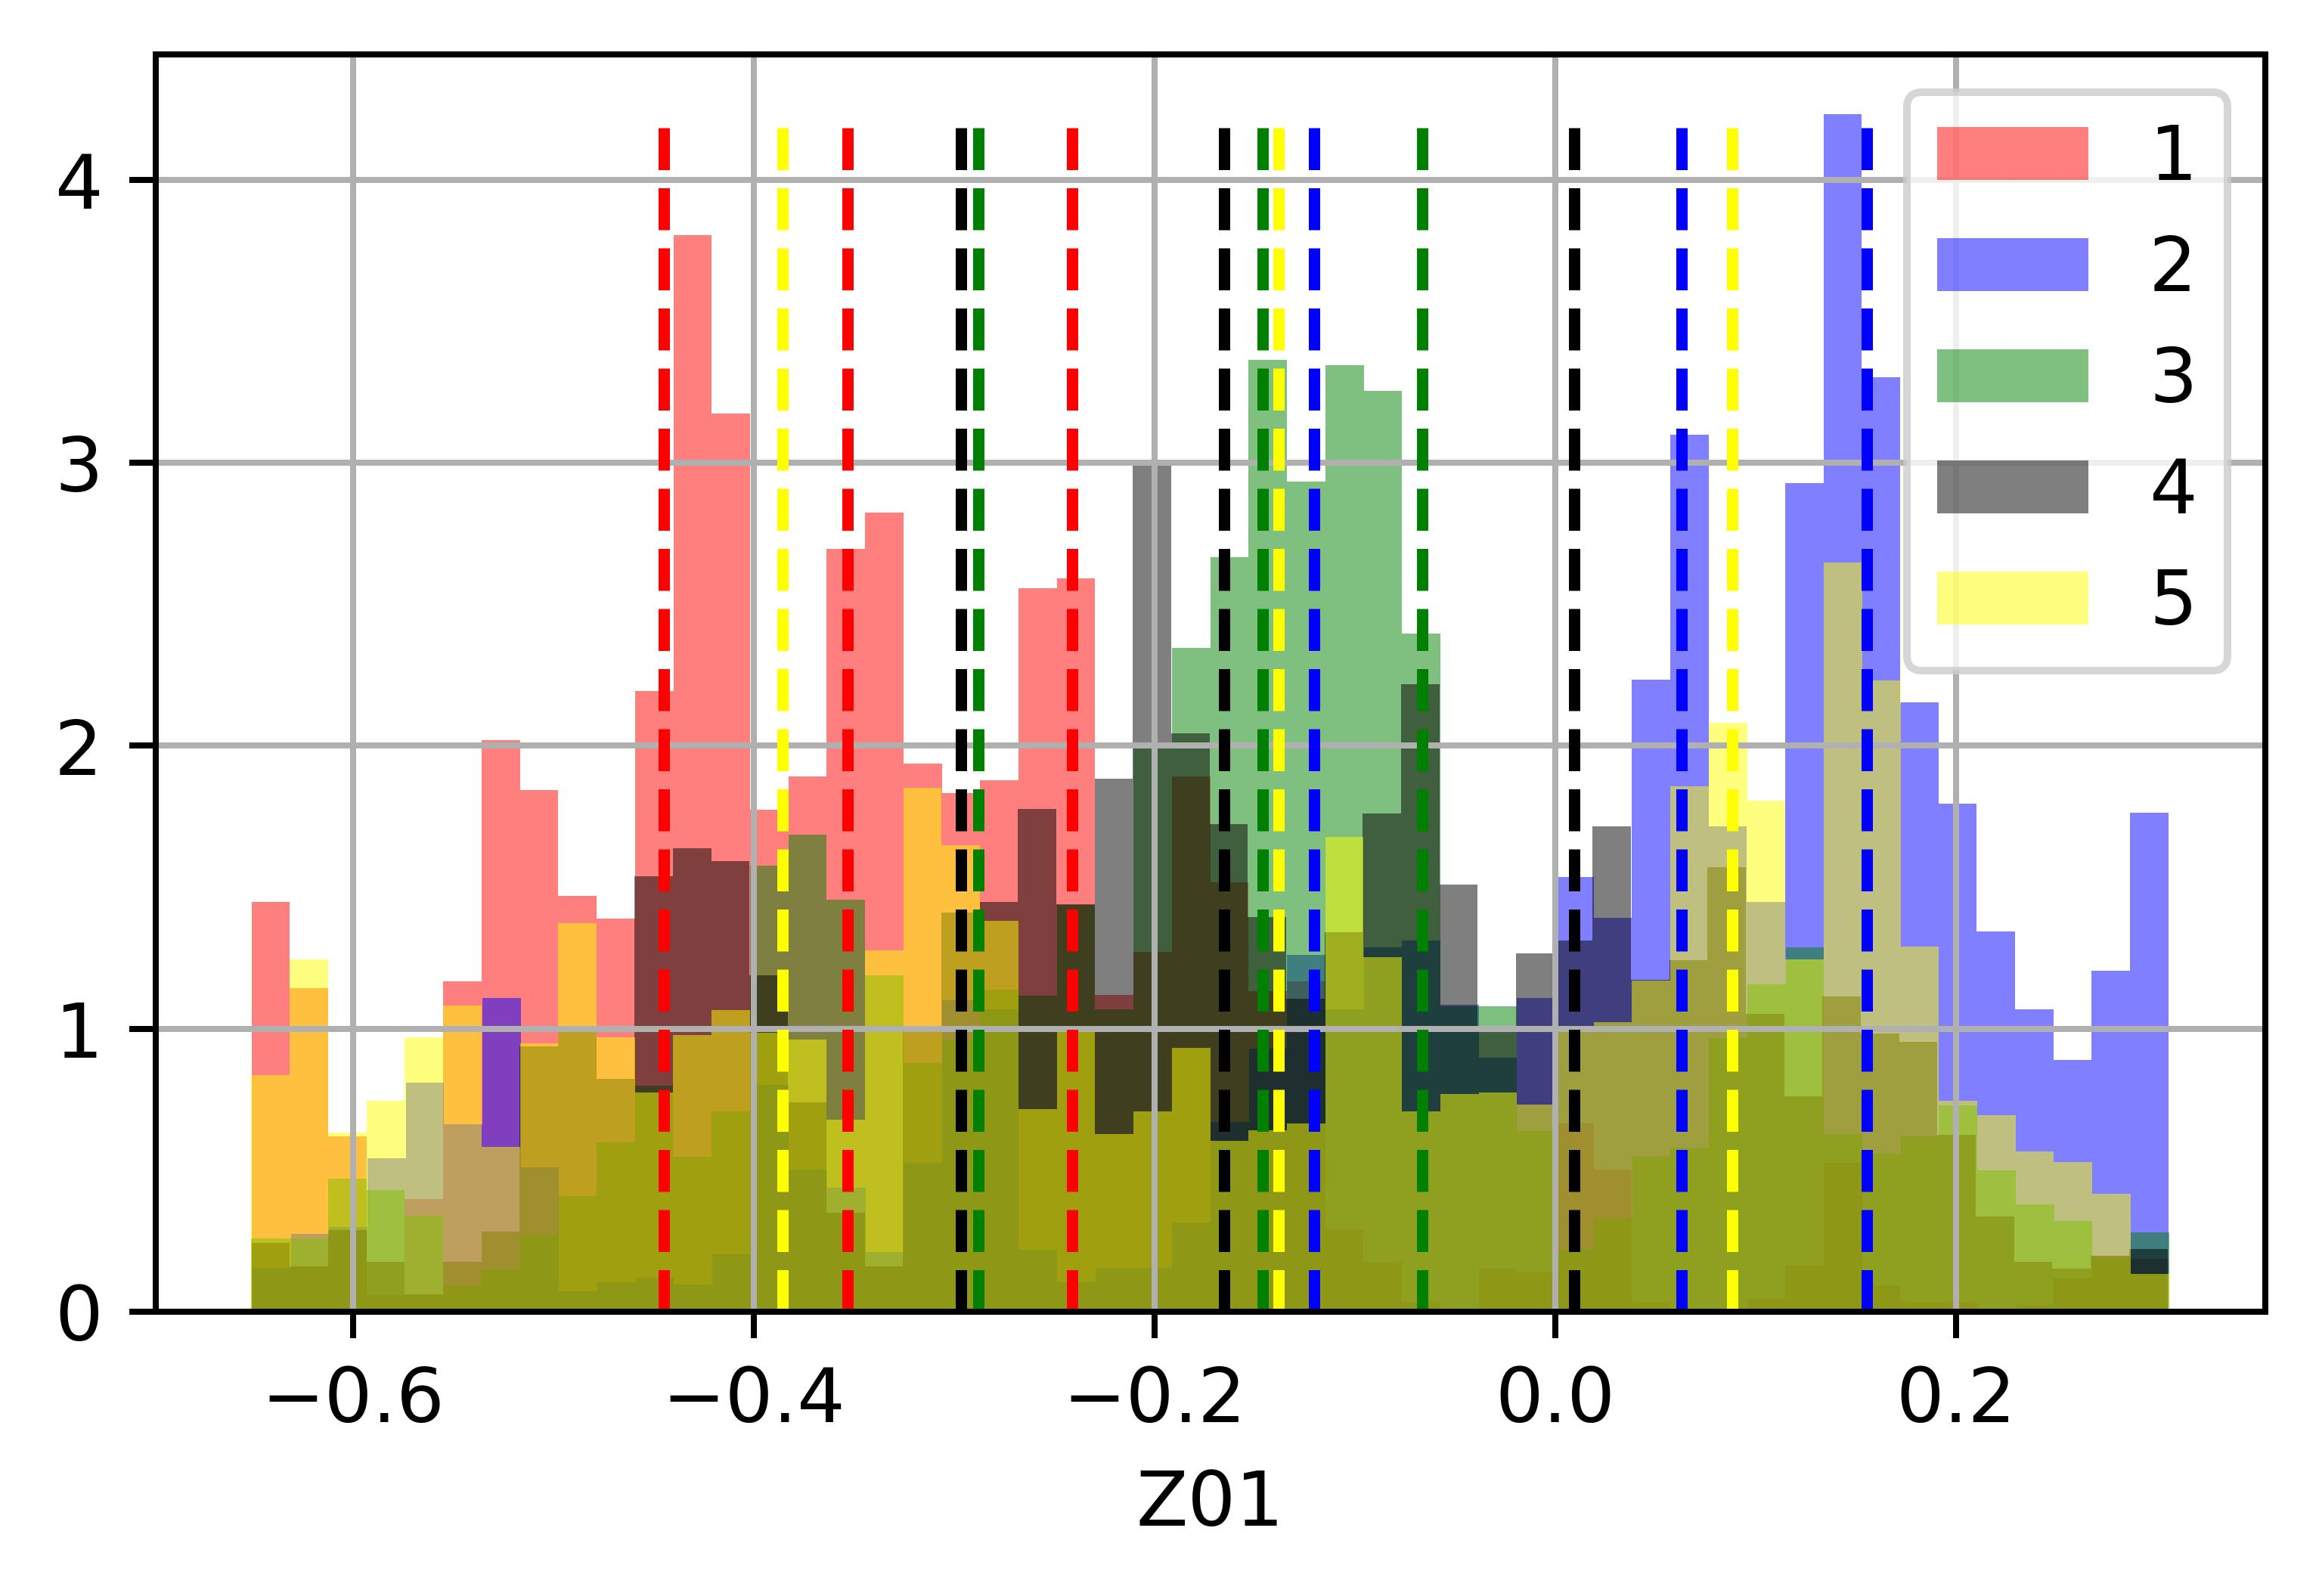
\includegraphics[width=0.18\textwidth]{../code/Task2/Analysis/Hist-Z01}
  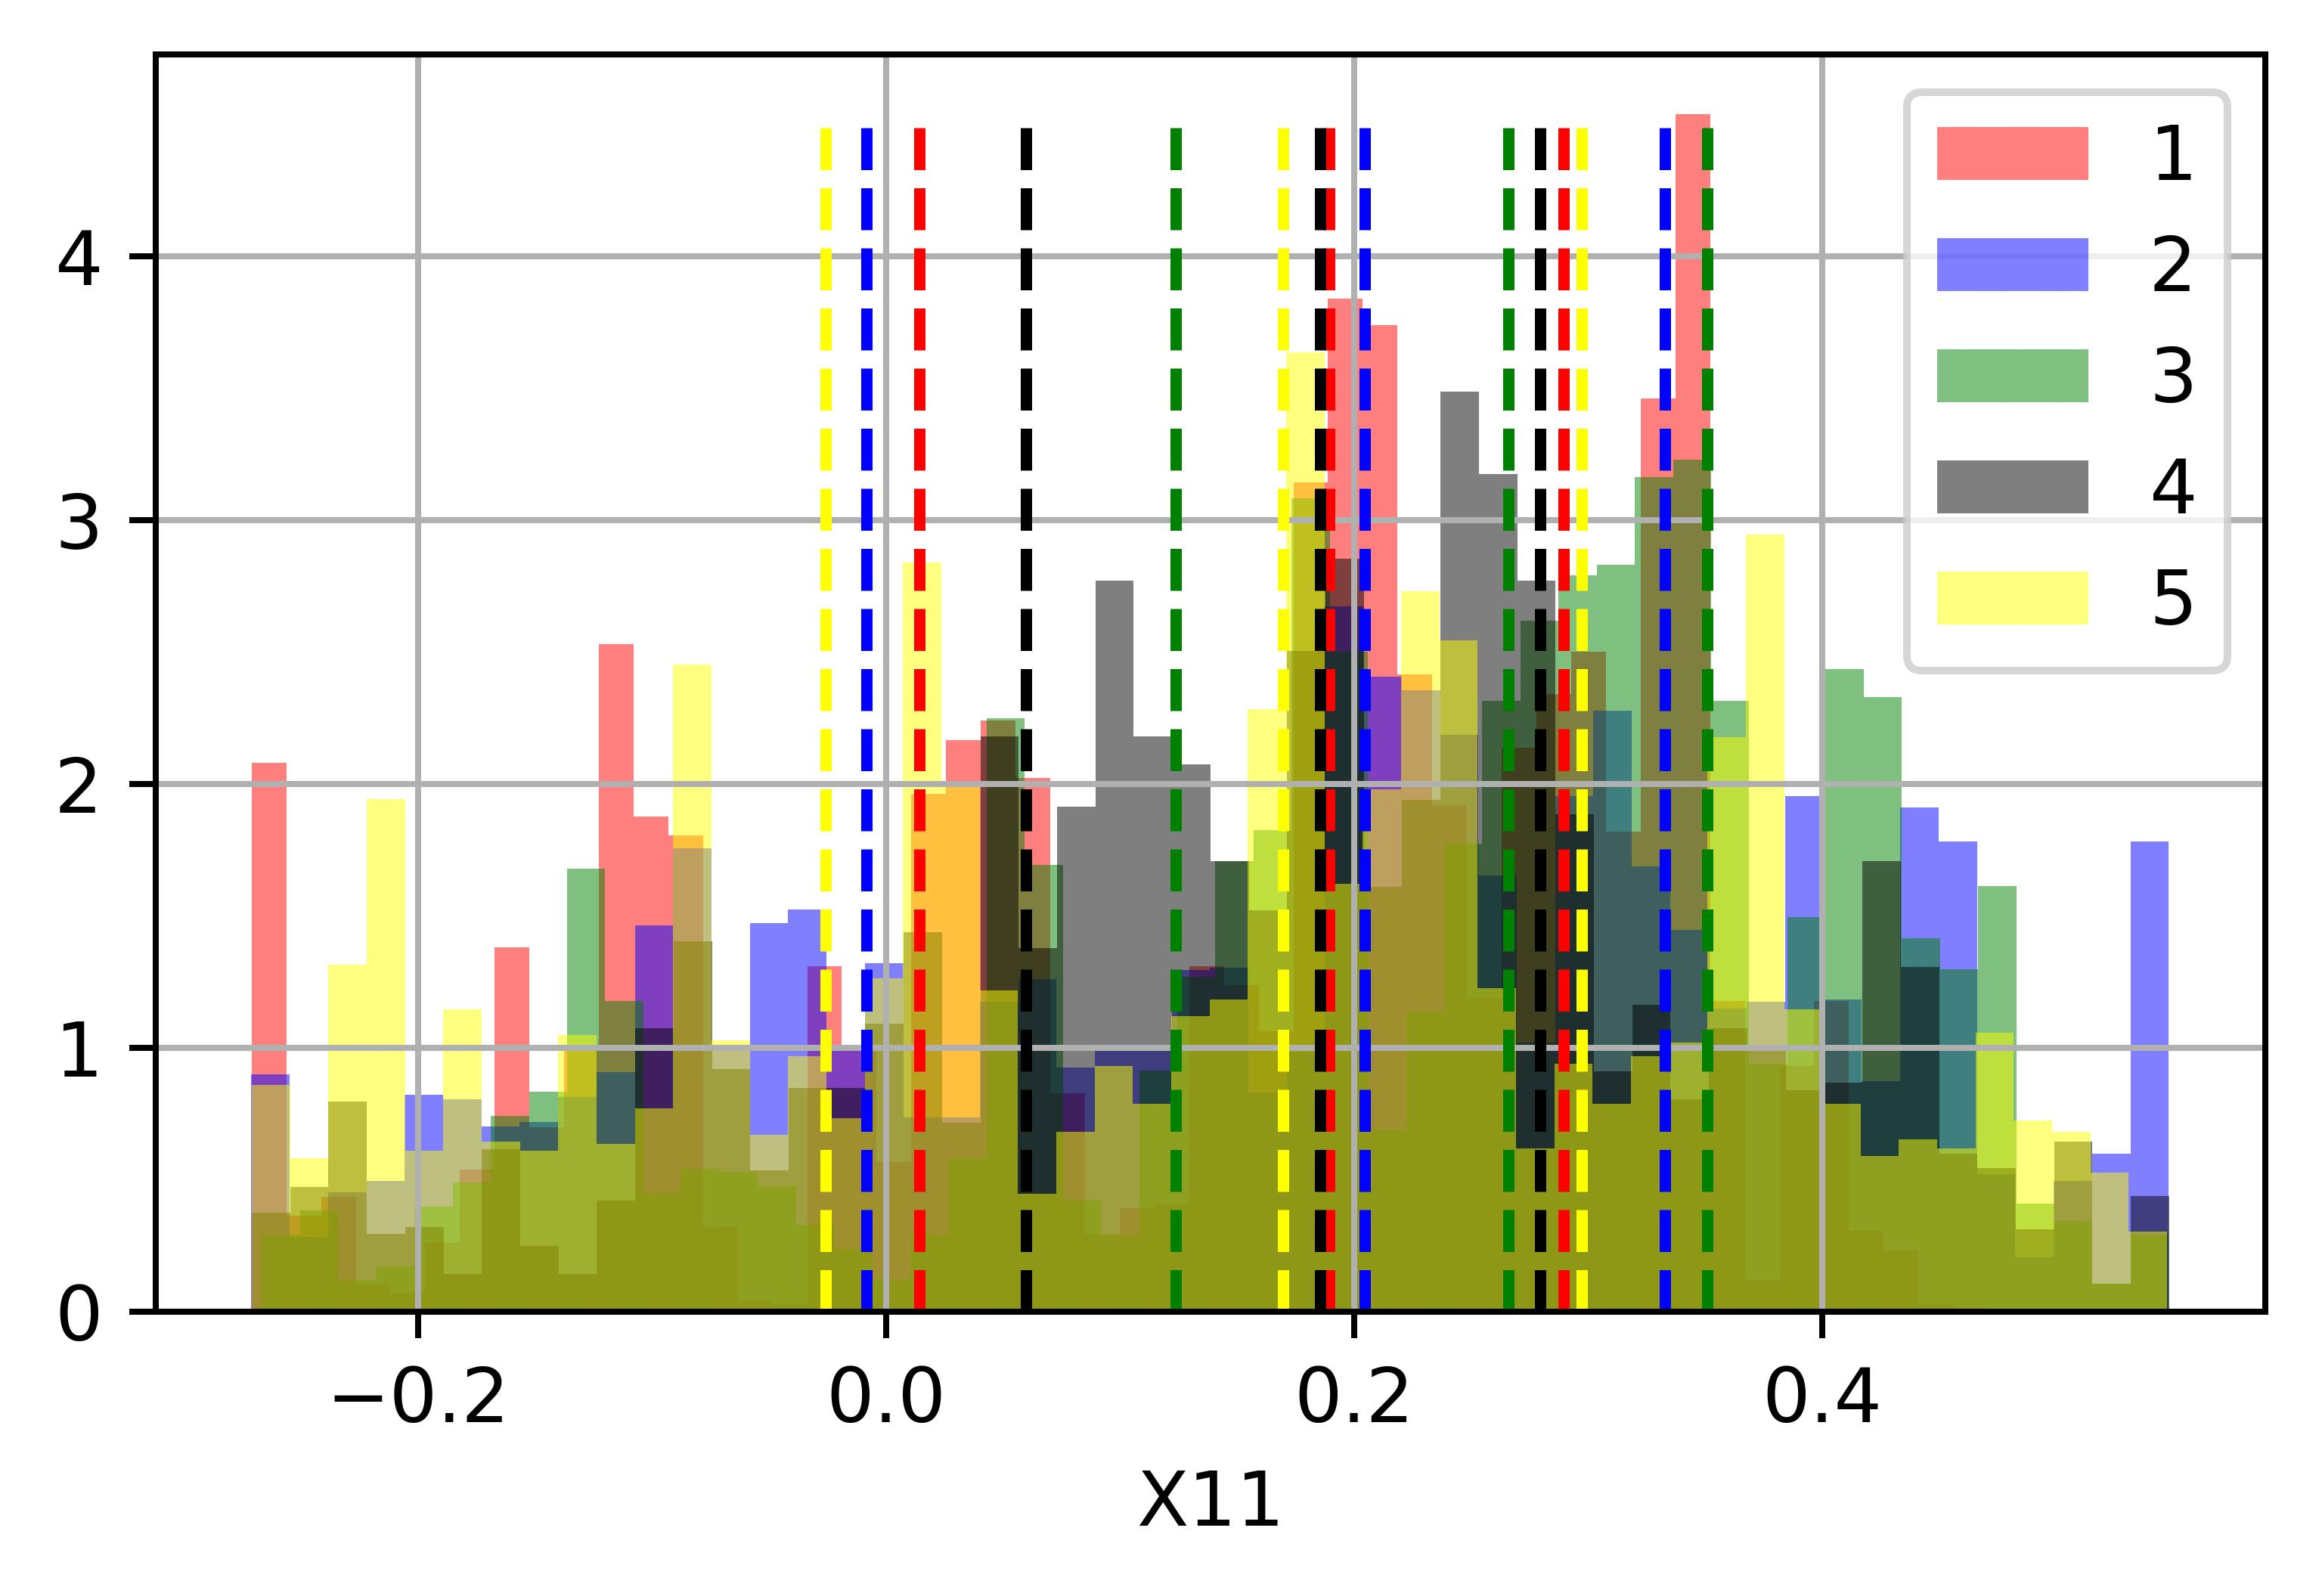
\includegraphics[width=0.18\textwidth]{../code/Task2/Analysis/Hist-X11}
  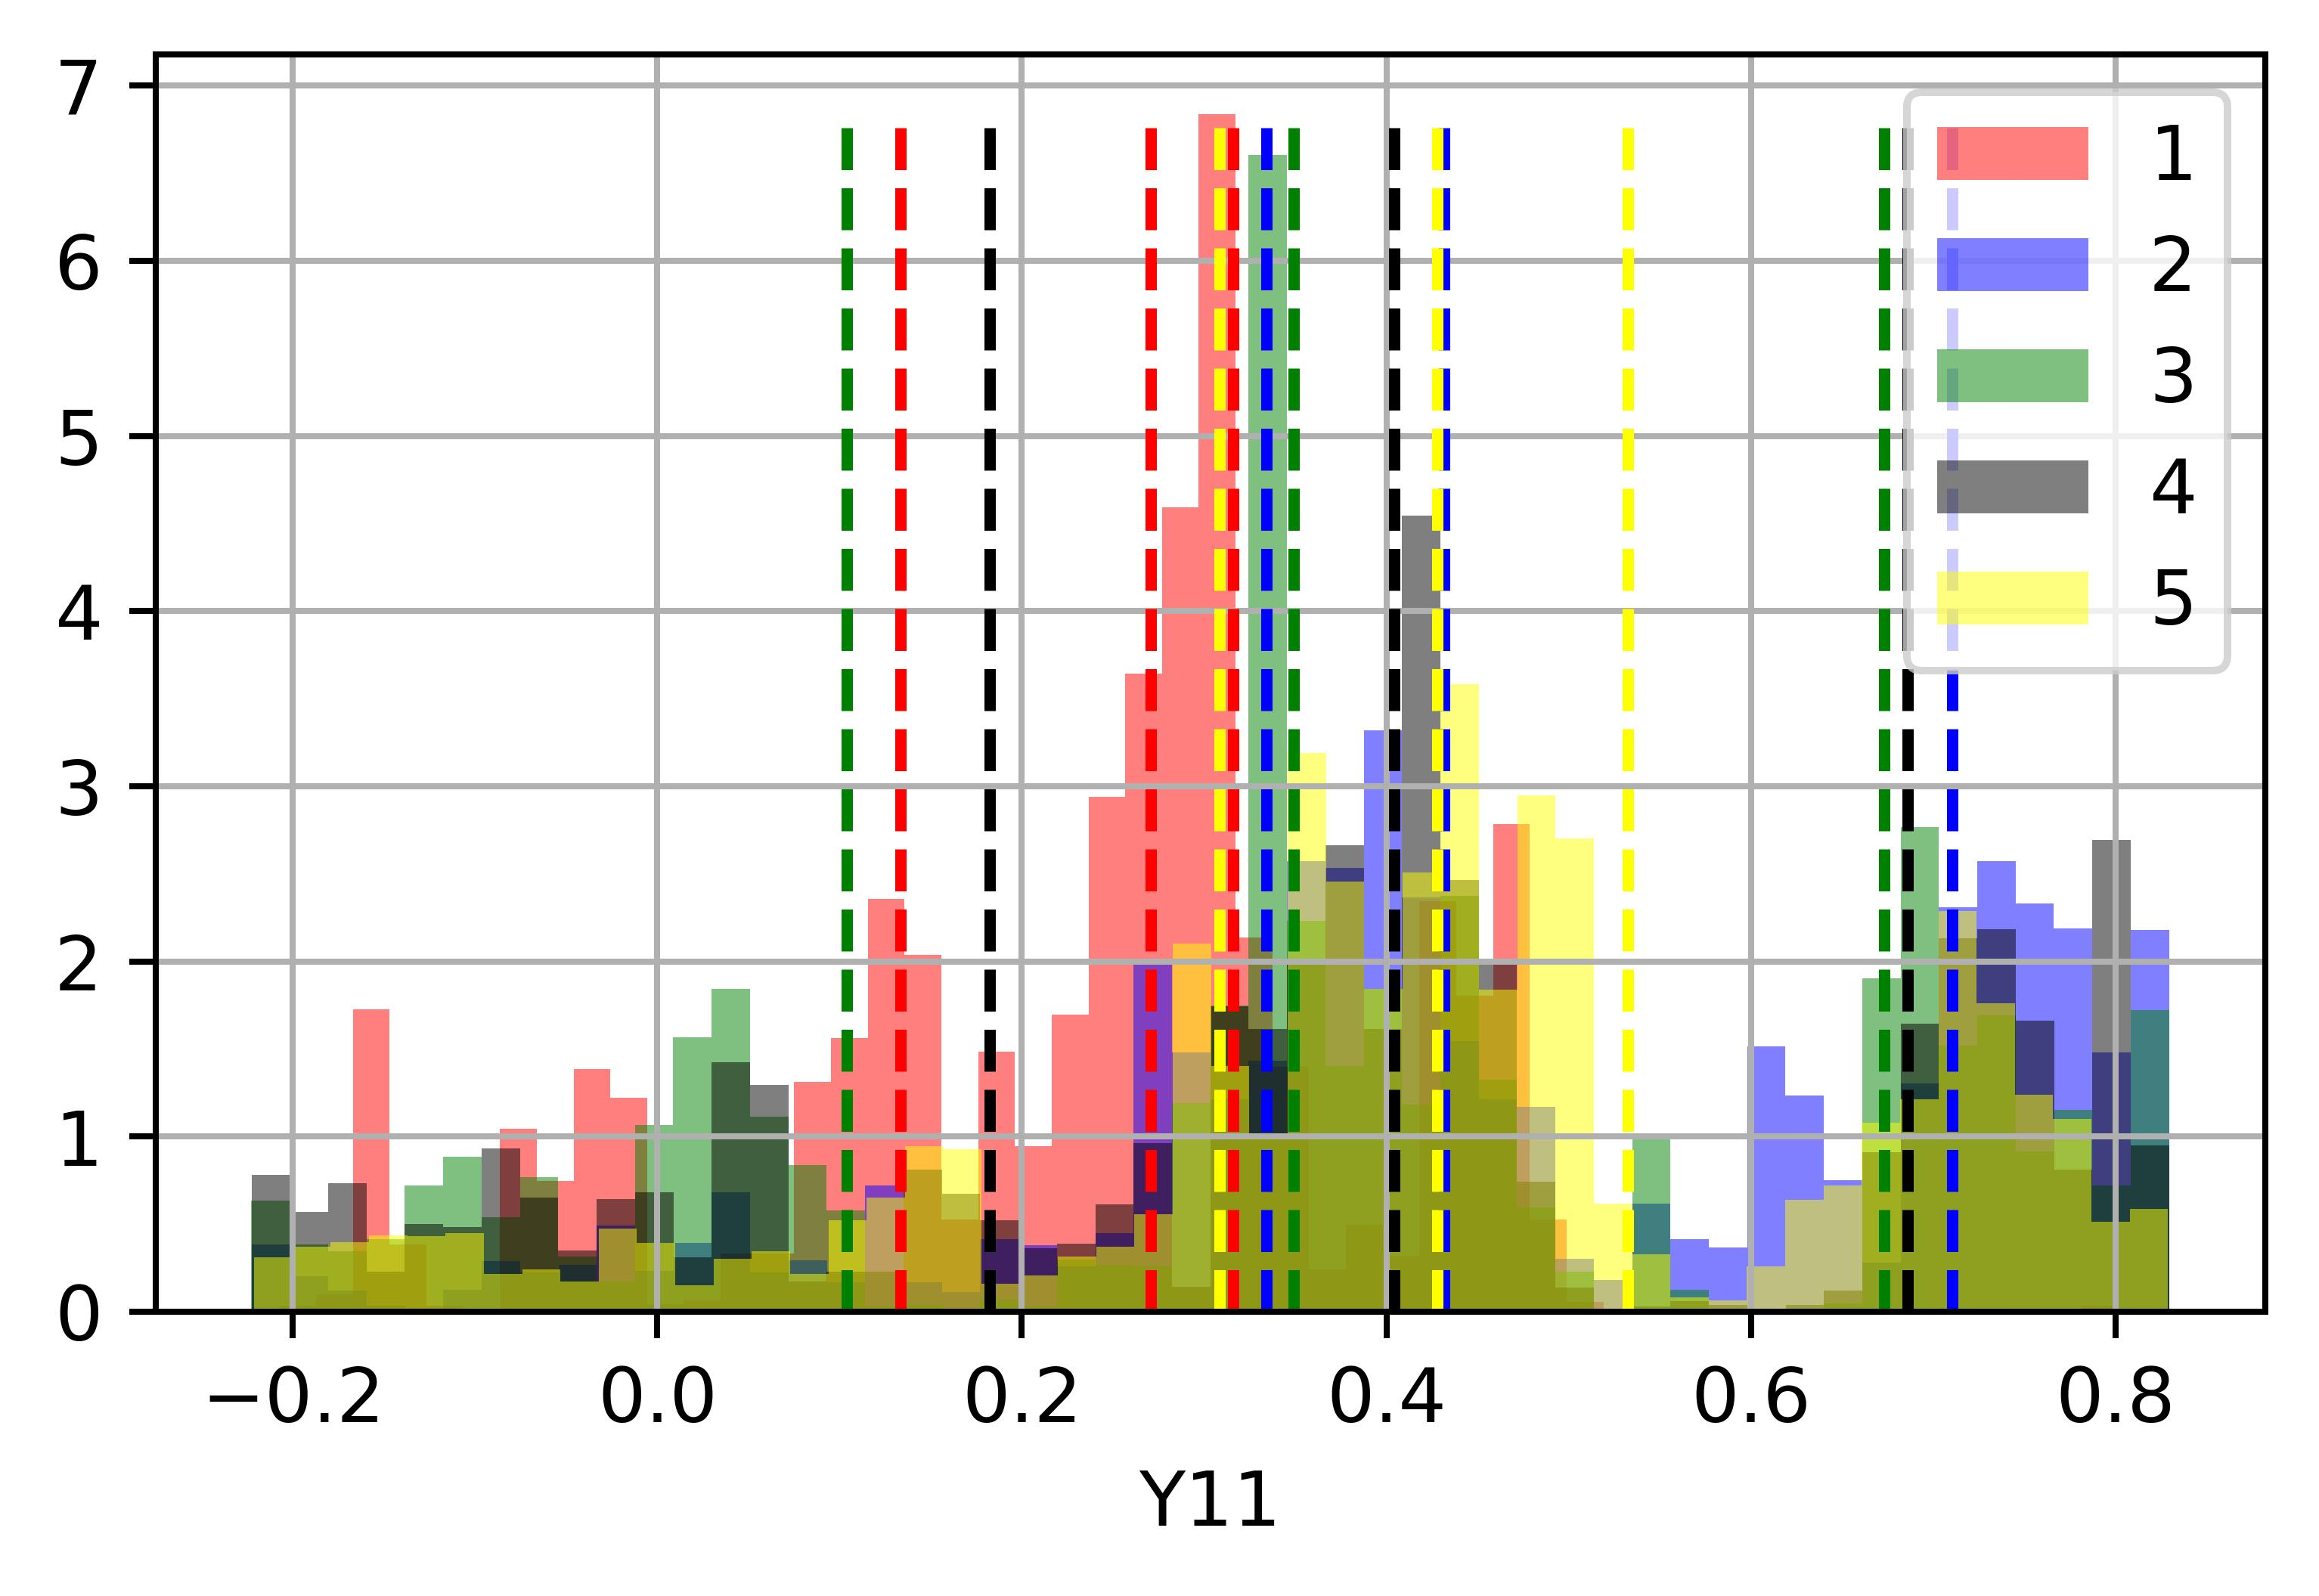
\includegraphics[width=0.18\textwidth]{../code/Task2/Analysis/Hist-Y11} \\
  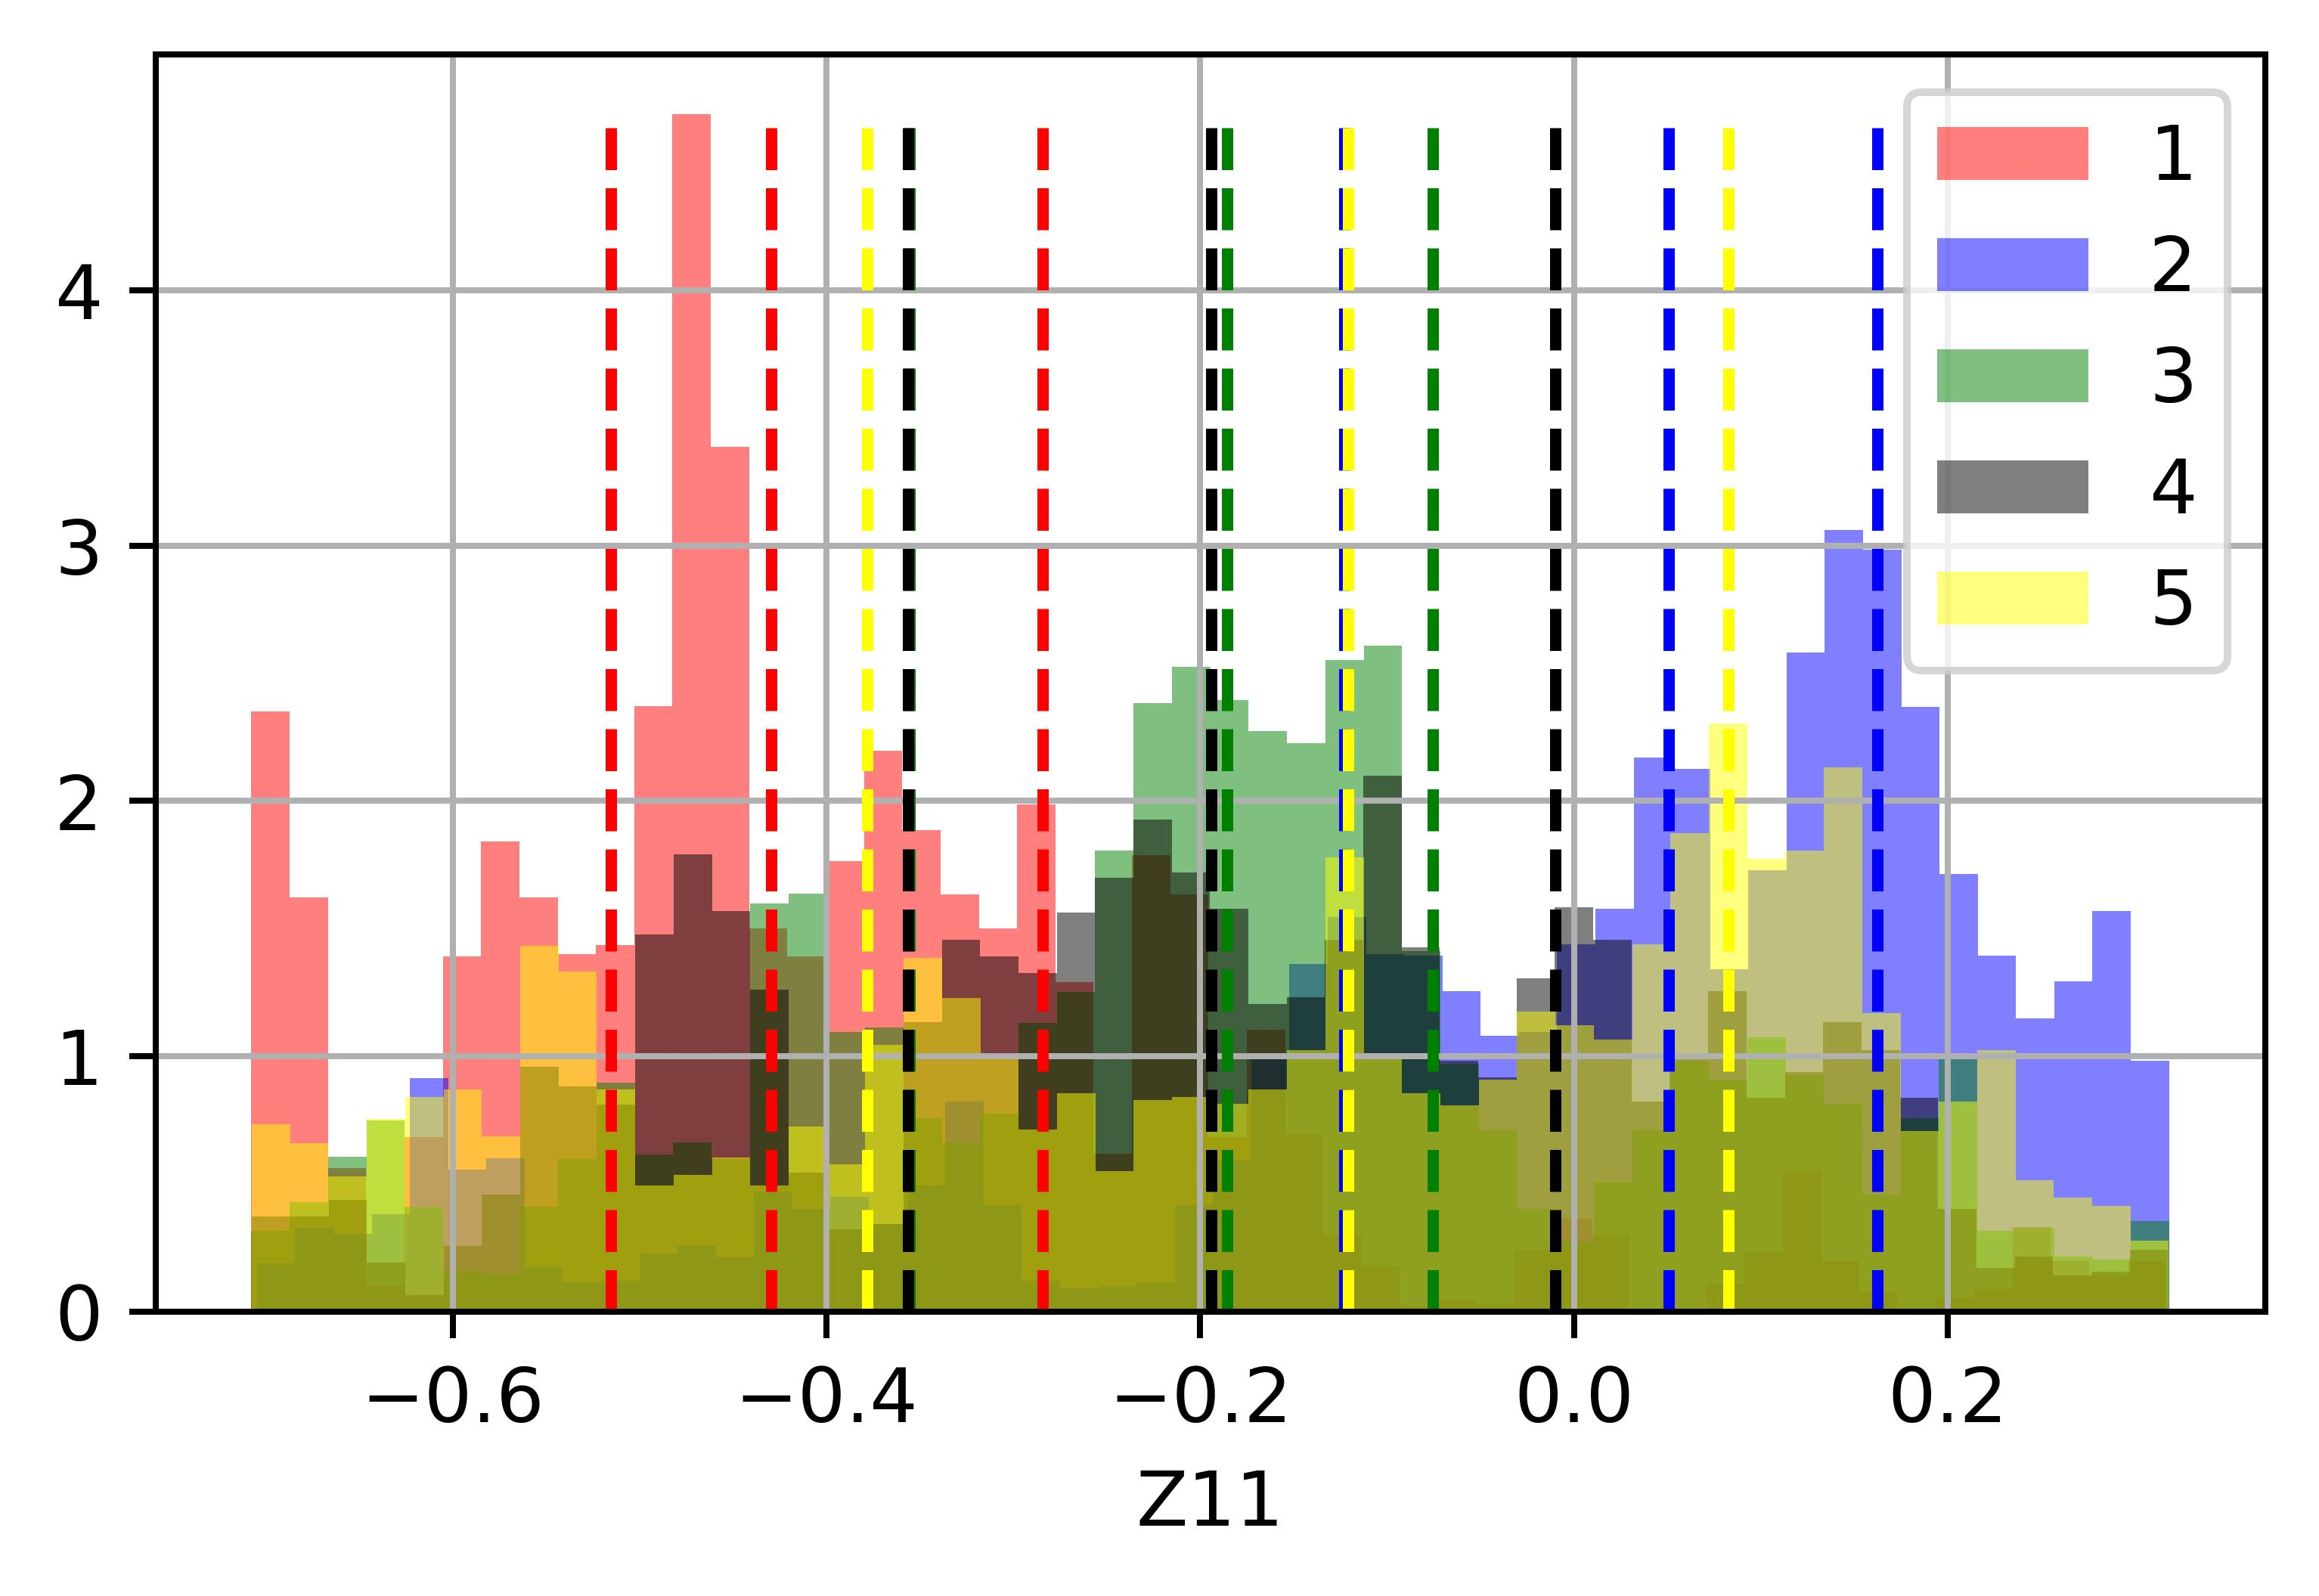
\includegraphics[width=0.18\textwidth]{../code/Task2/Analysis/Hist-Z11}
  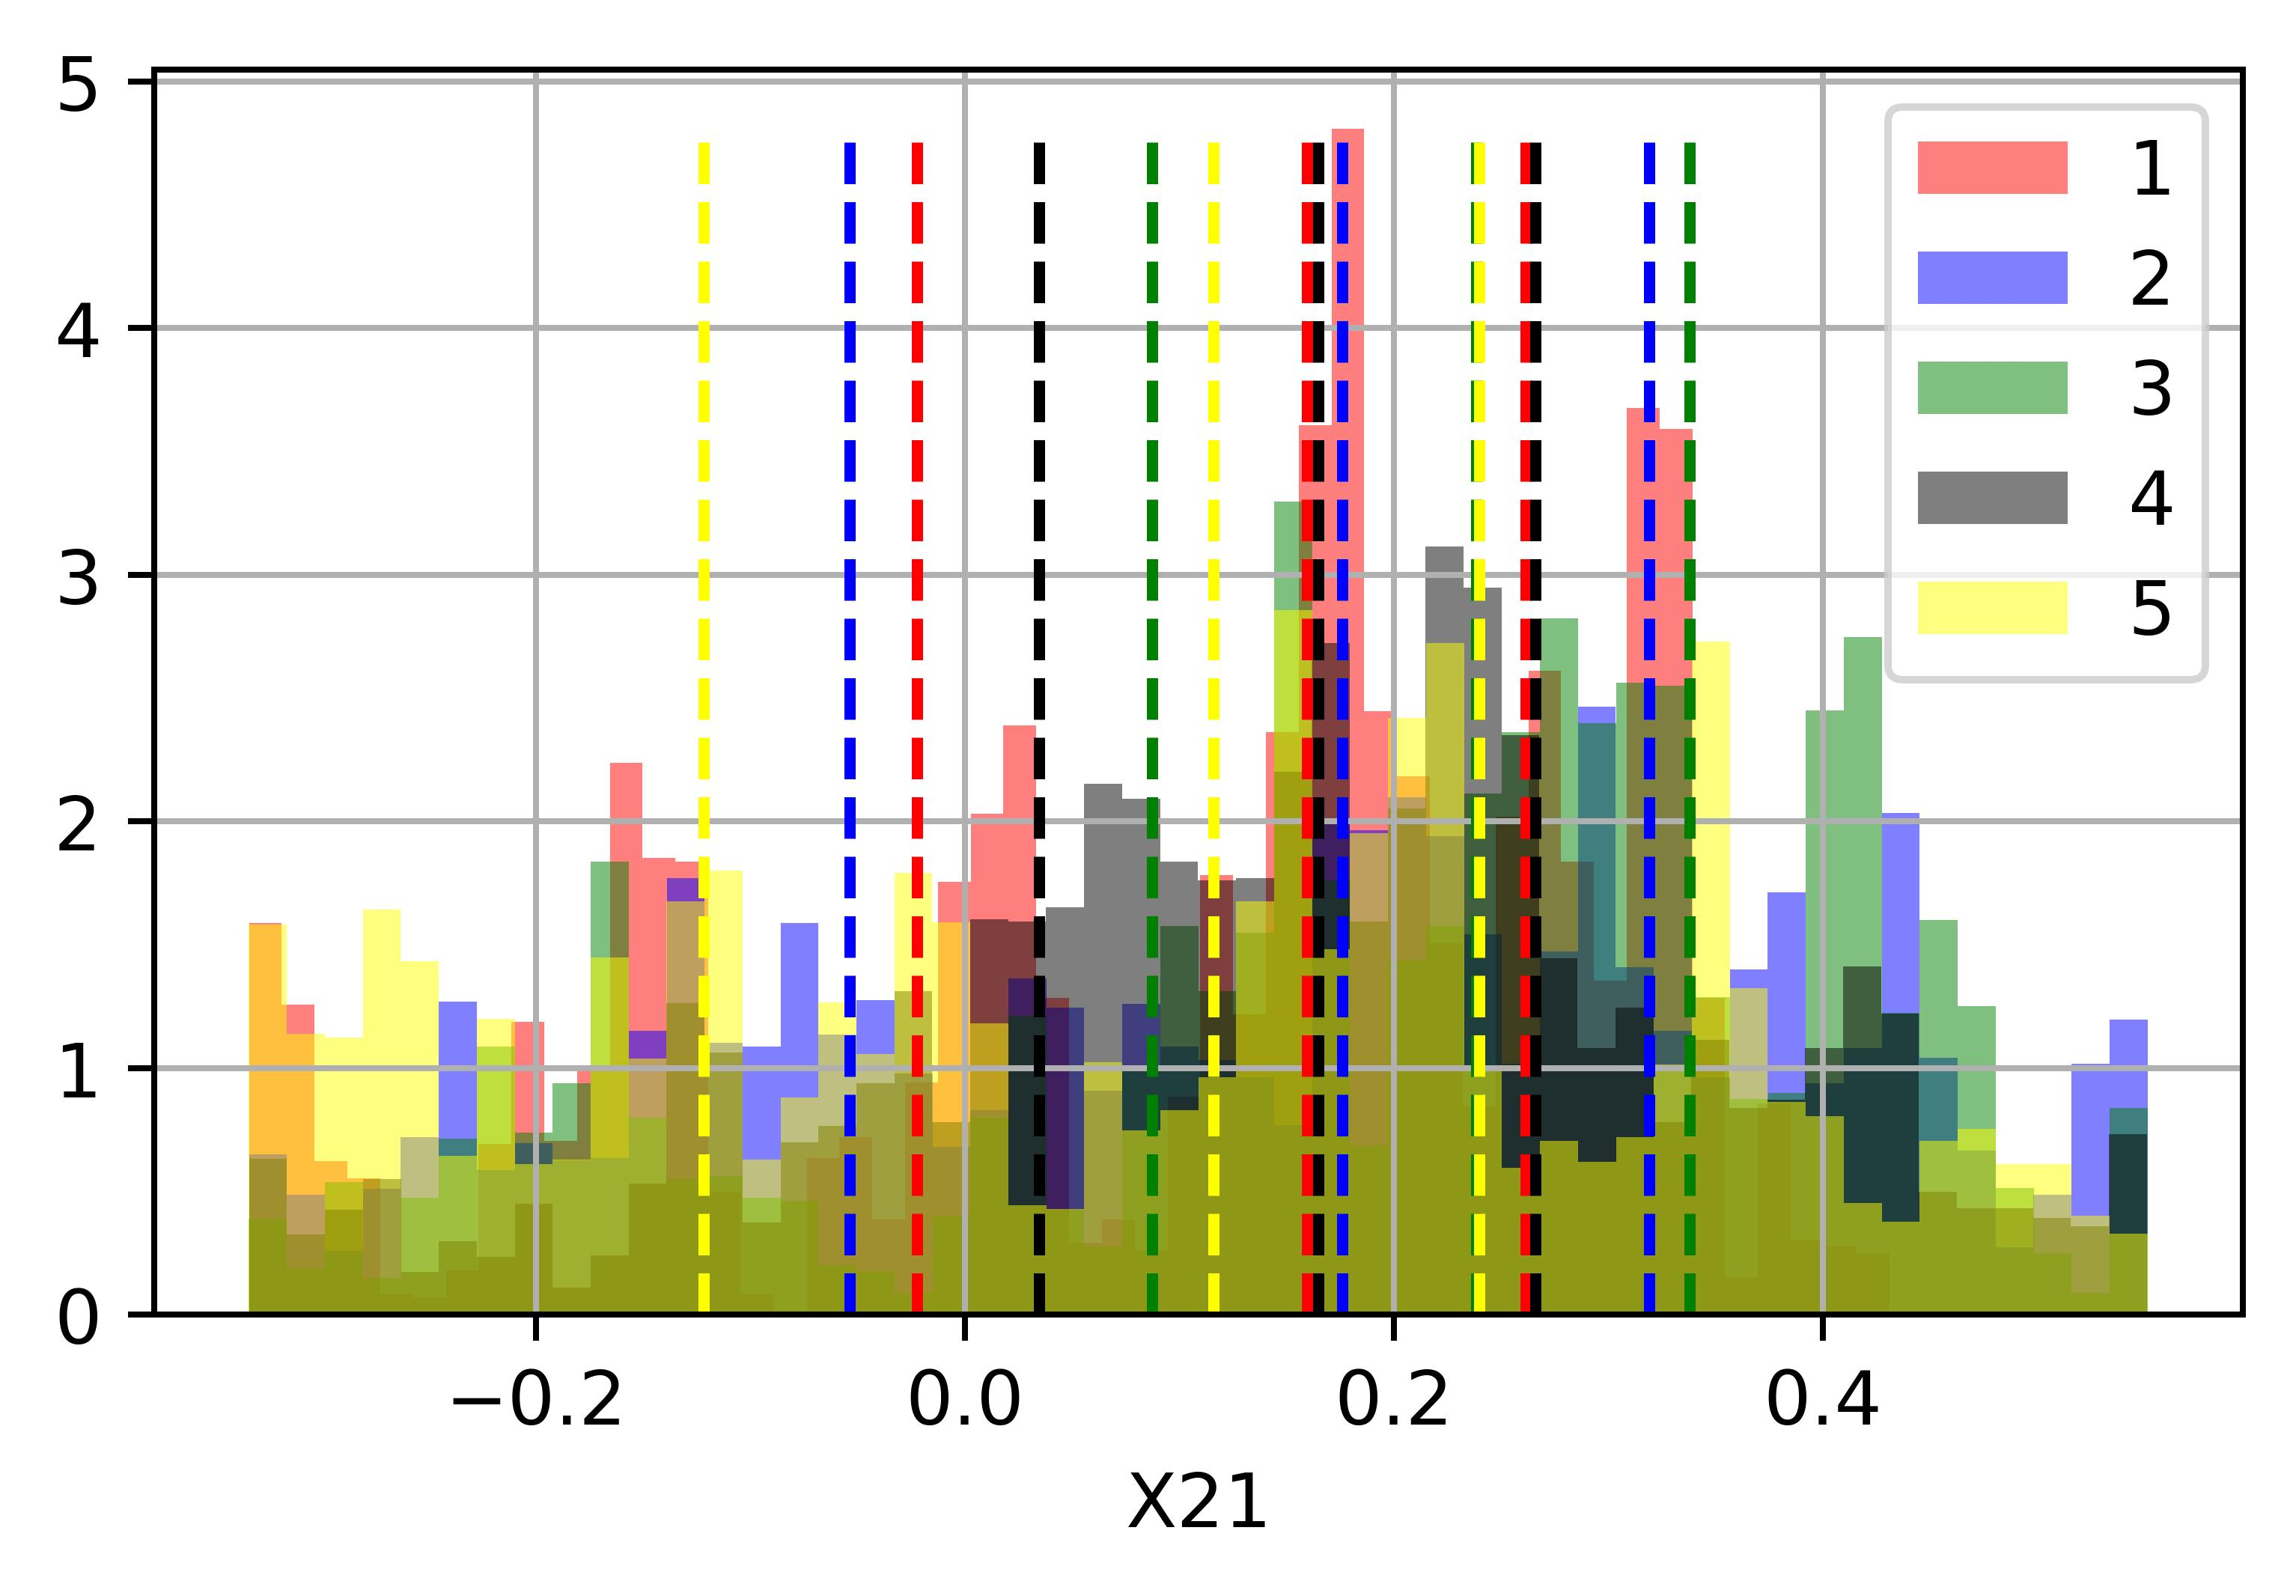
\includegraphics[width=0.18\textwidth]{../code/Task2/Analysis/Hist-X21}
  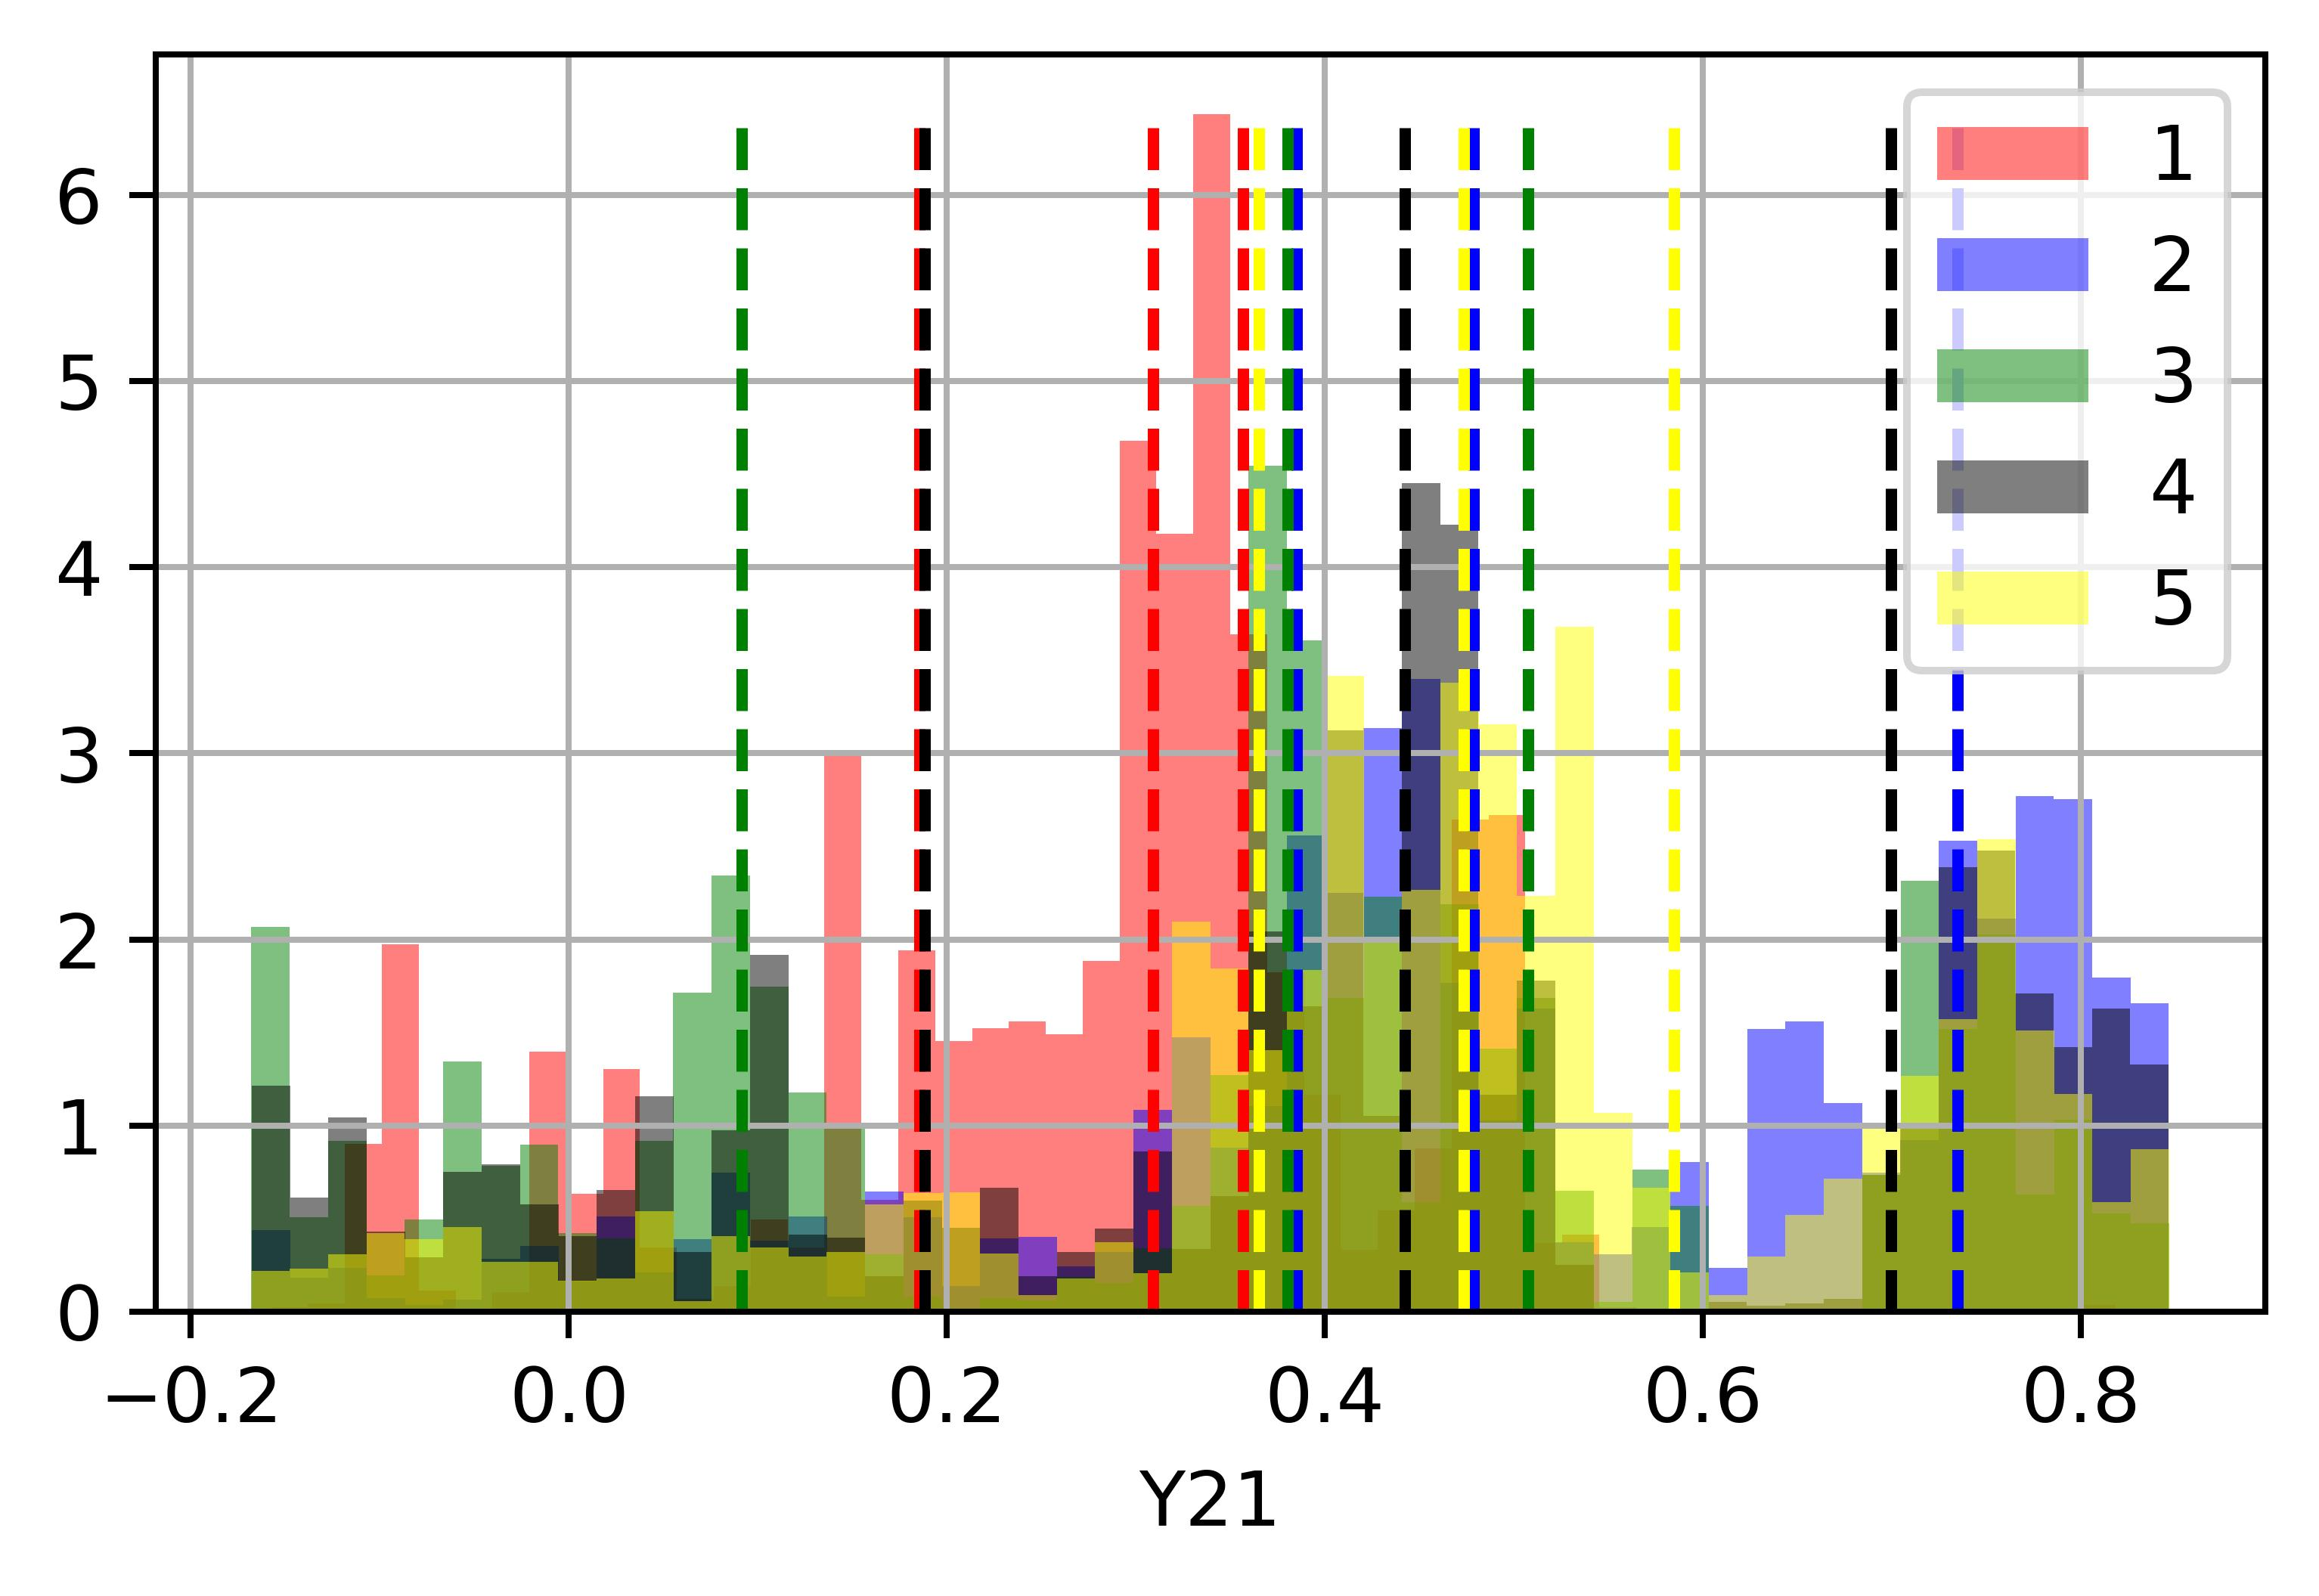
\includegraphics[width=0.18\textwidth]{../code/Task2/Analysis/Hist-Y21}
  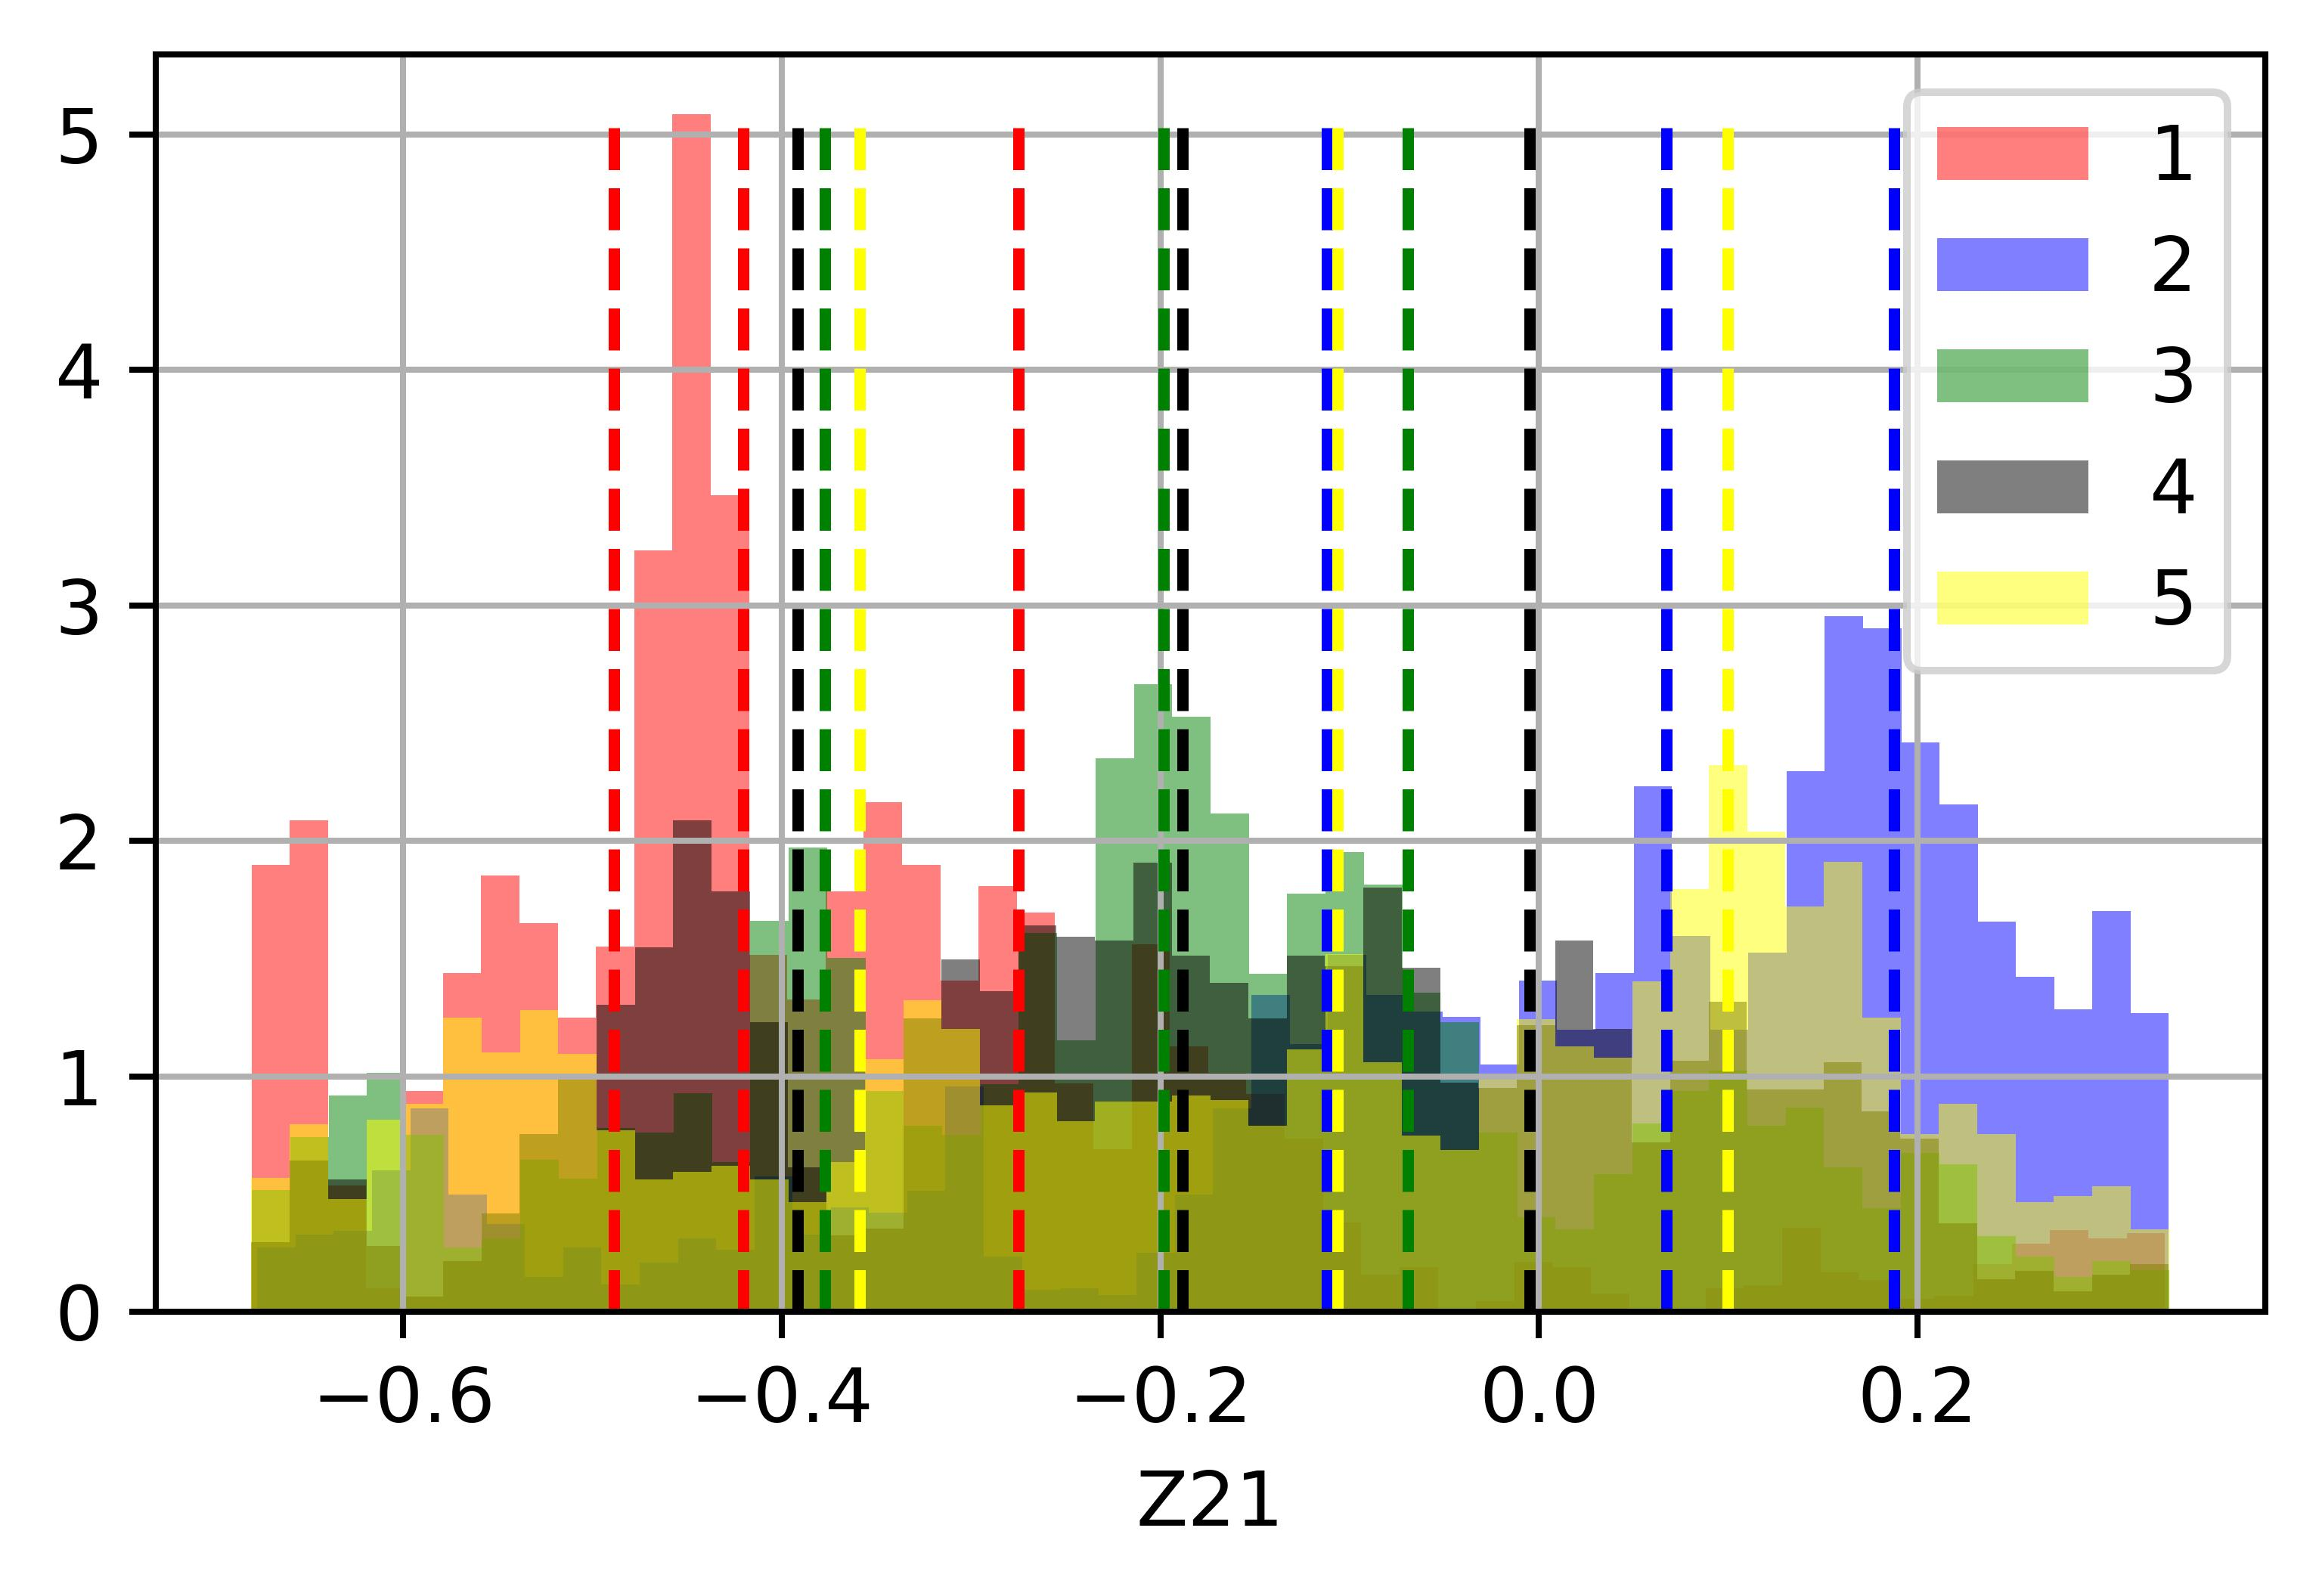
\includegraphics[width=0.18\textwidth]{../code/Task2/Analysis/Hist-Z21}
  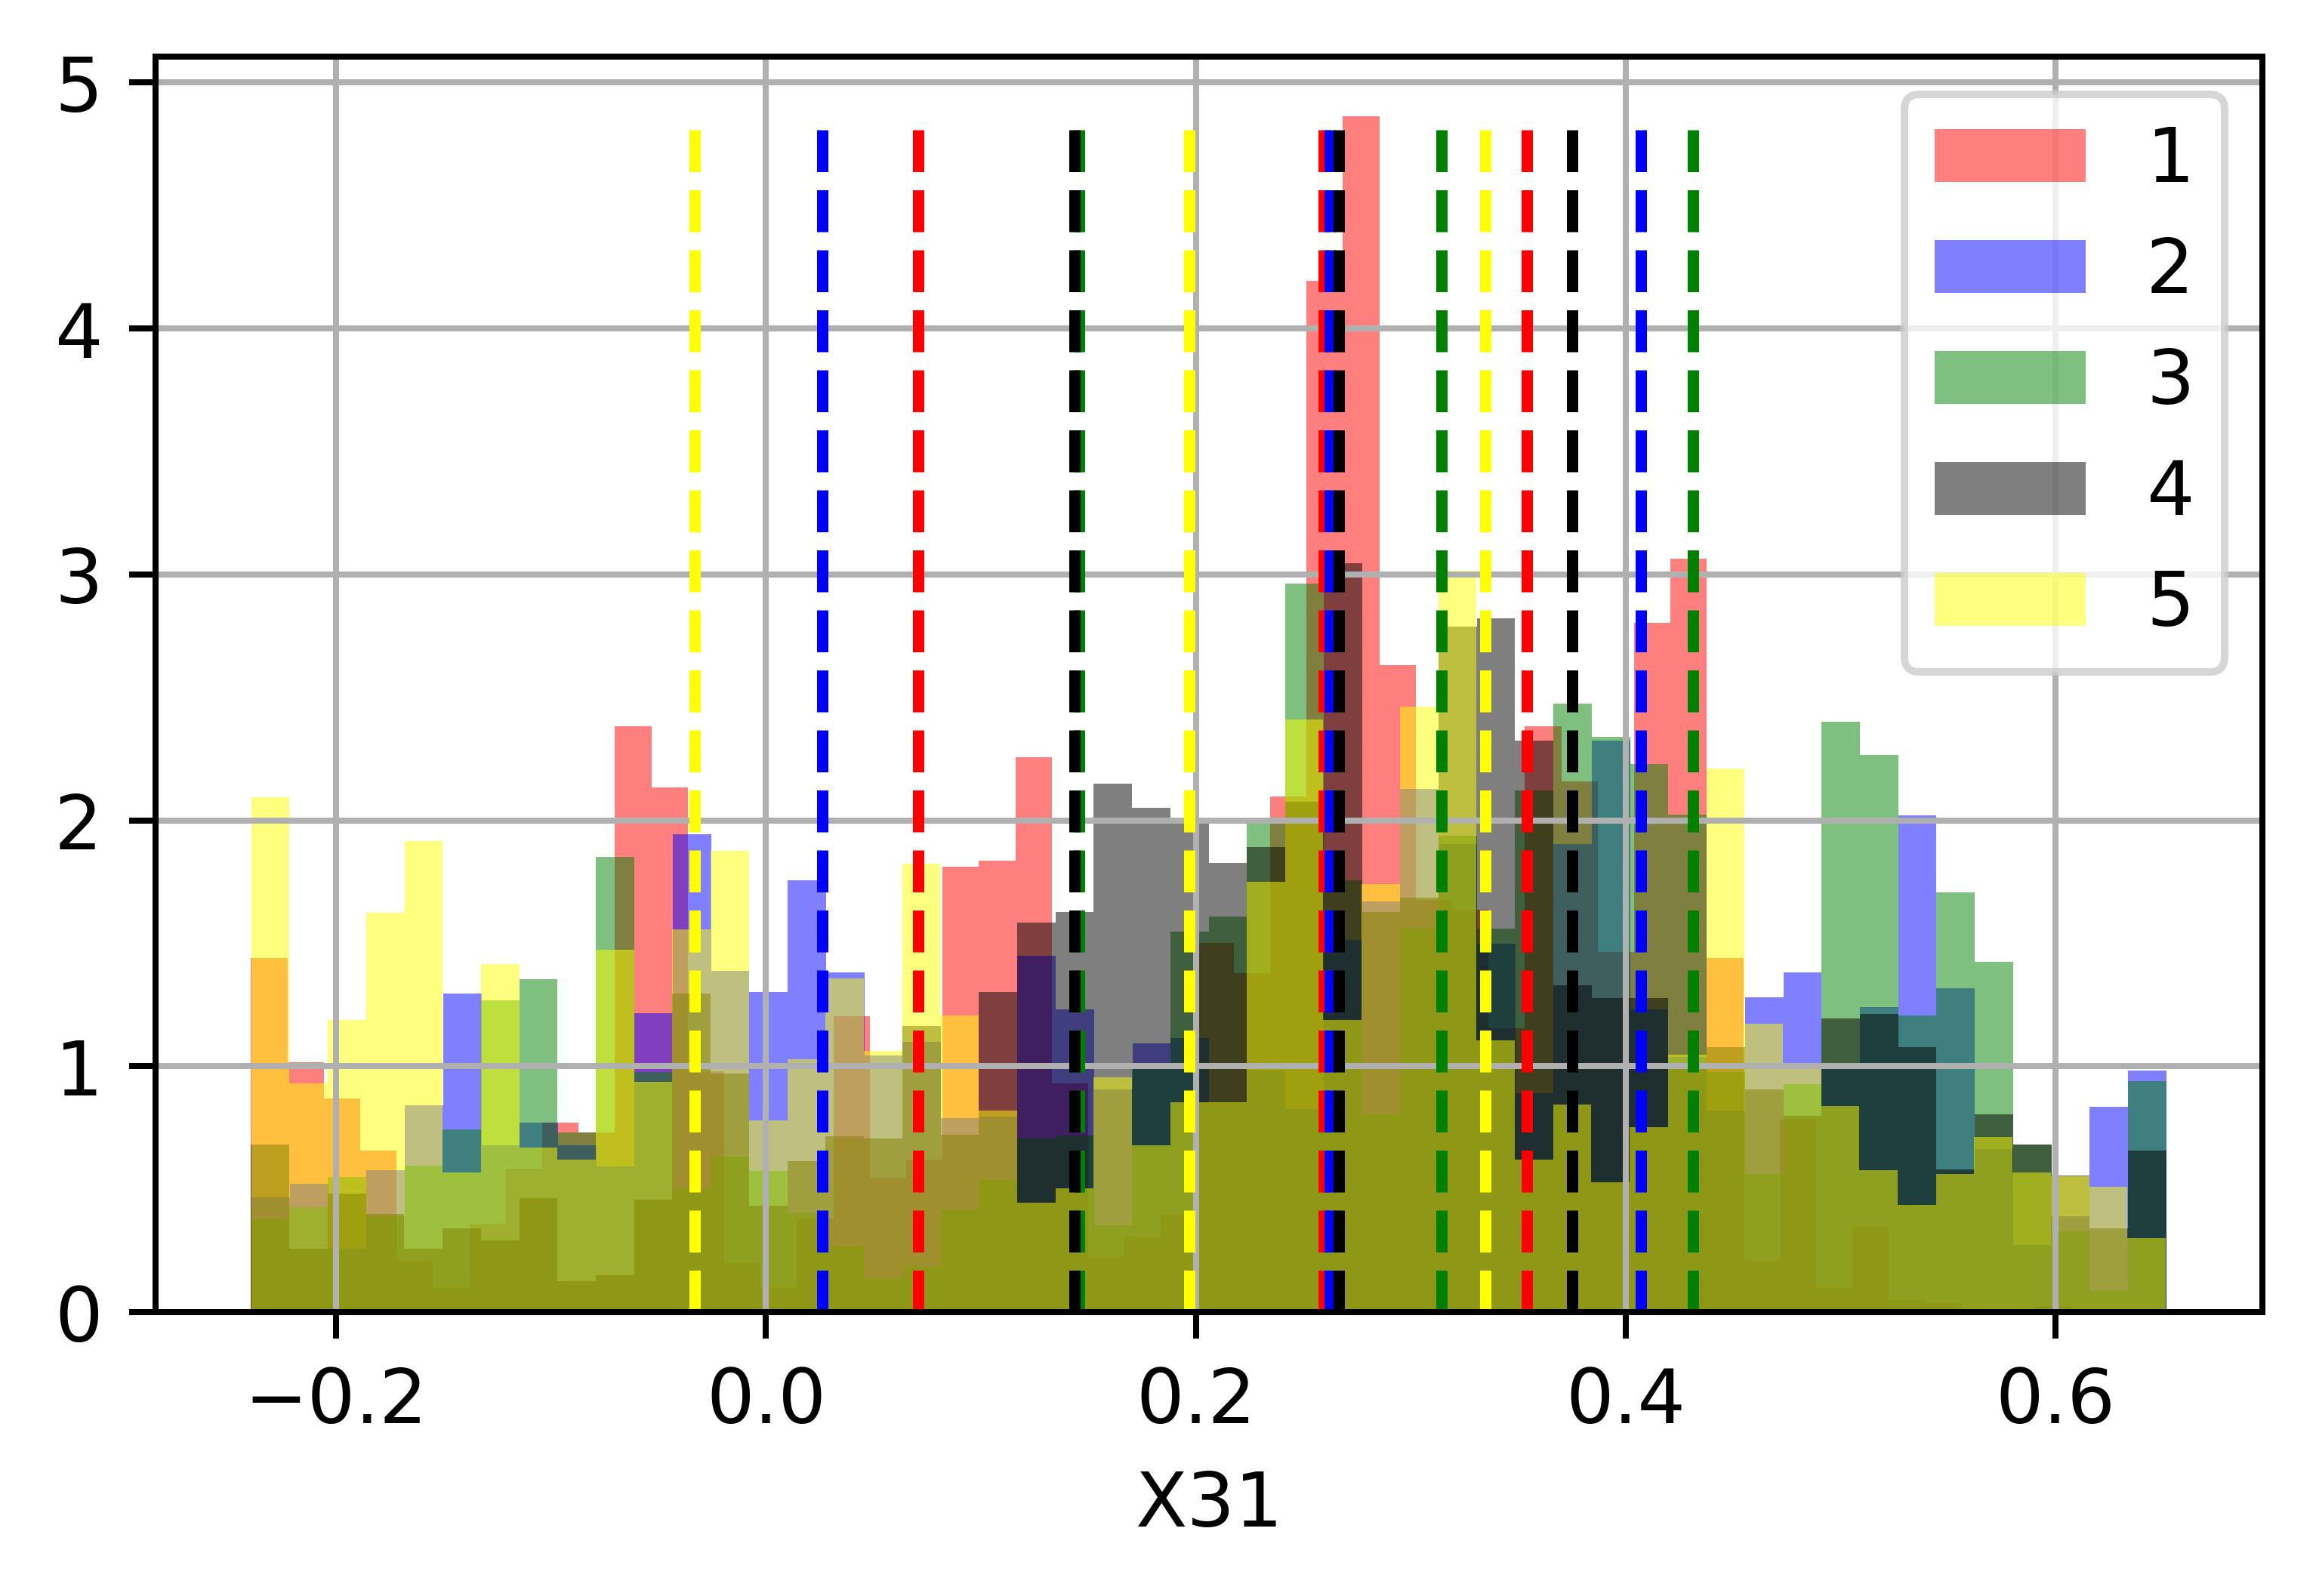
\includegraphics[width=0.18\textwidth]{../code/Task2/Analysis/Hist-X31} \\
  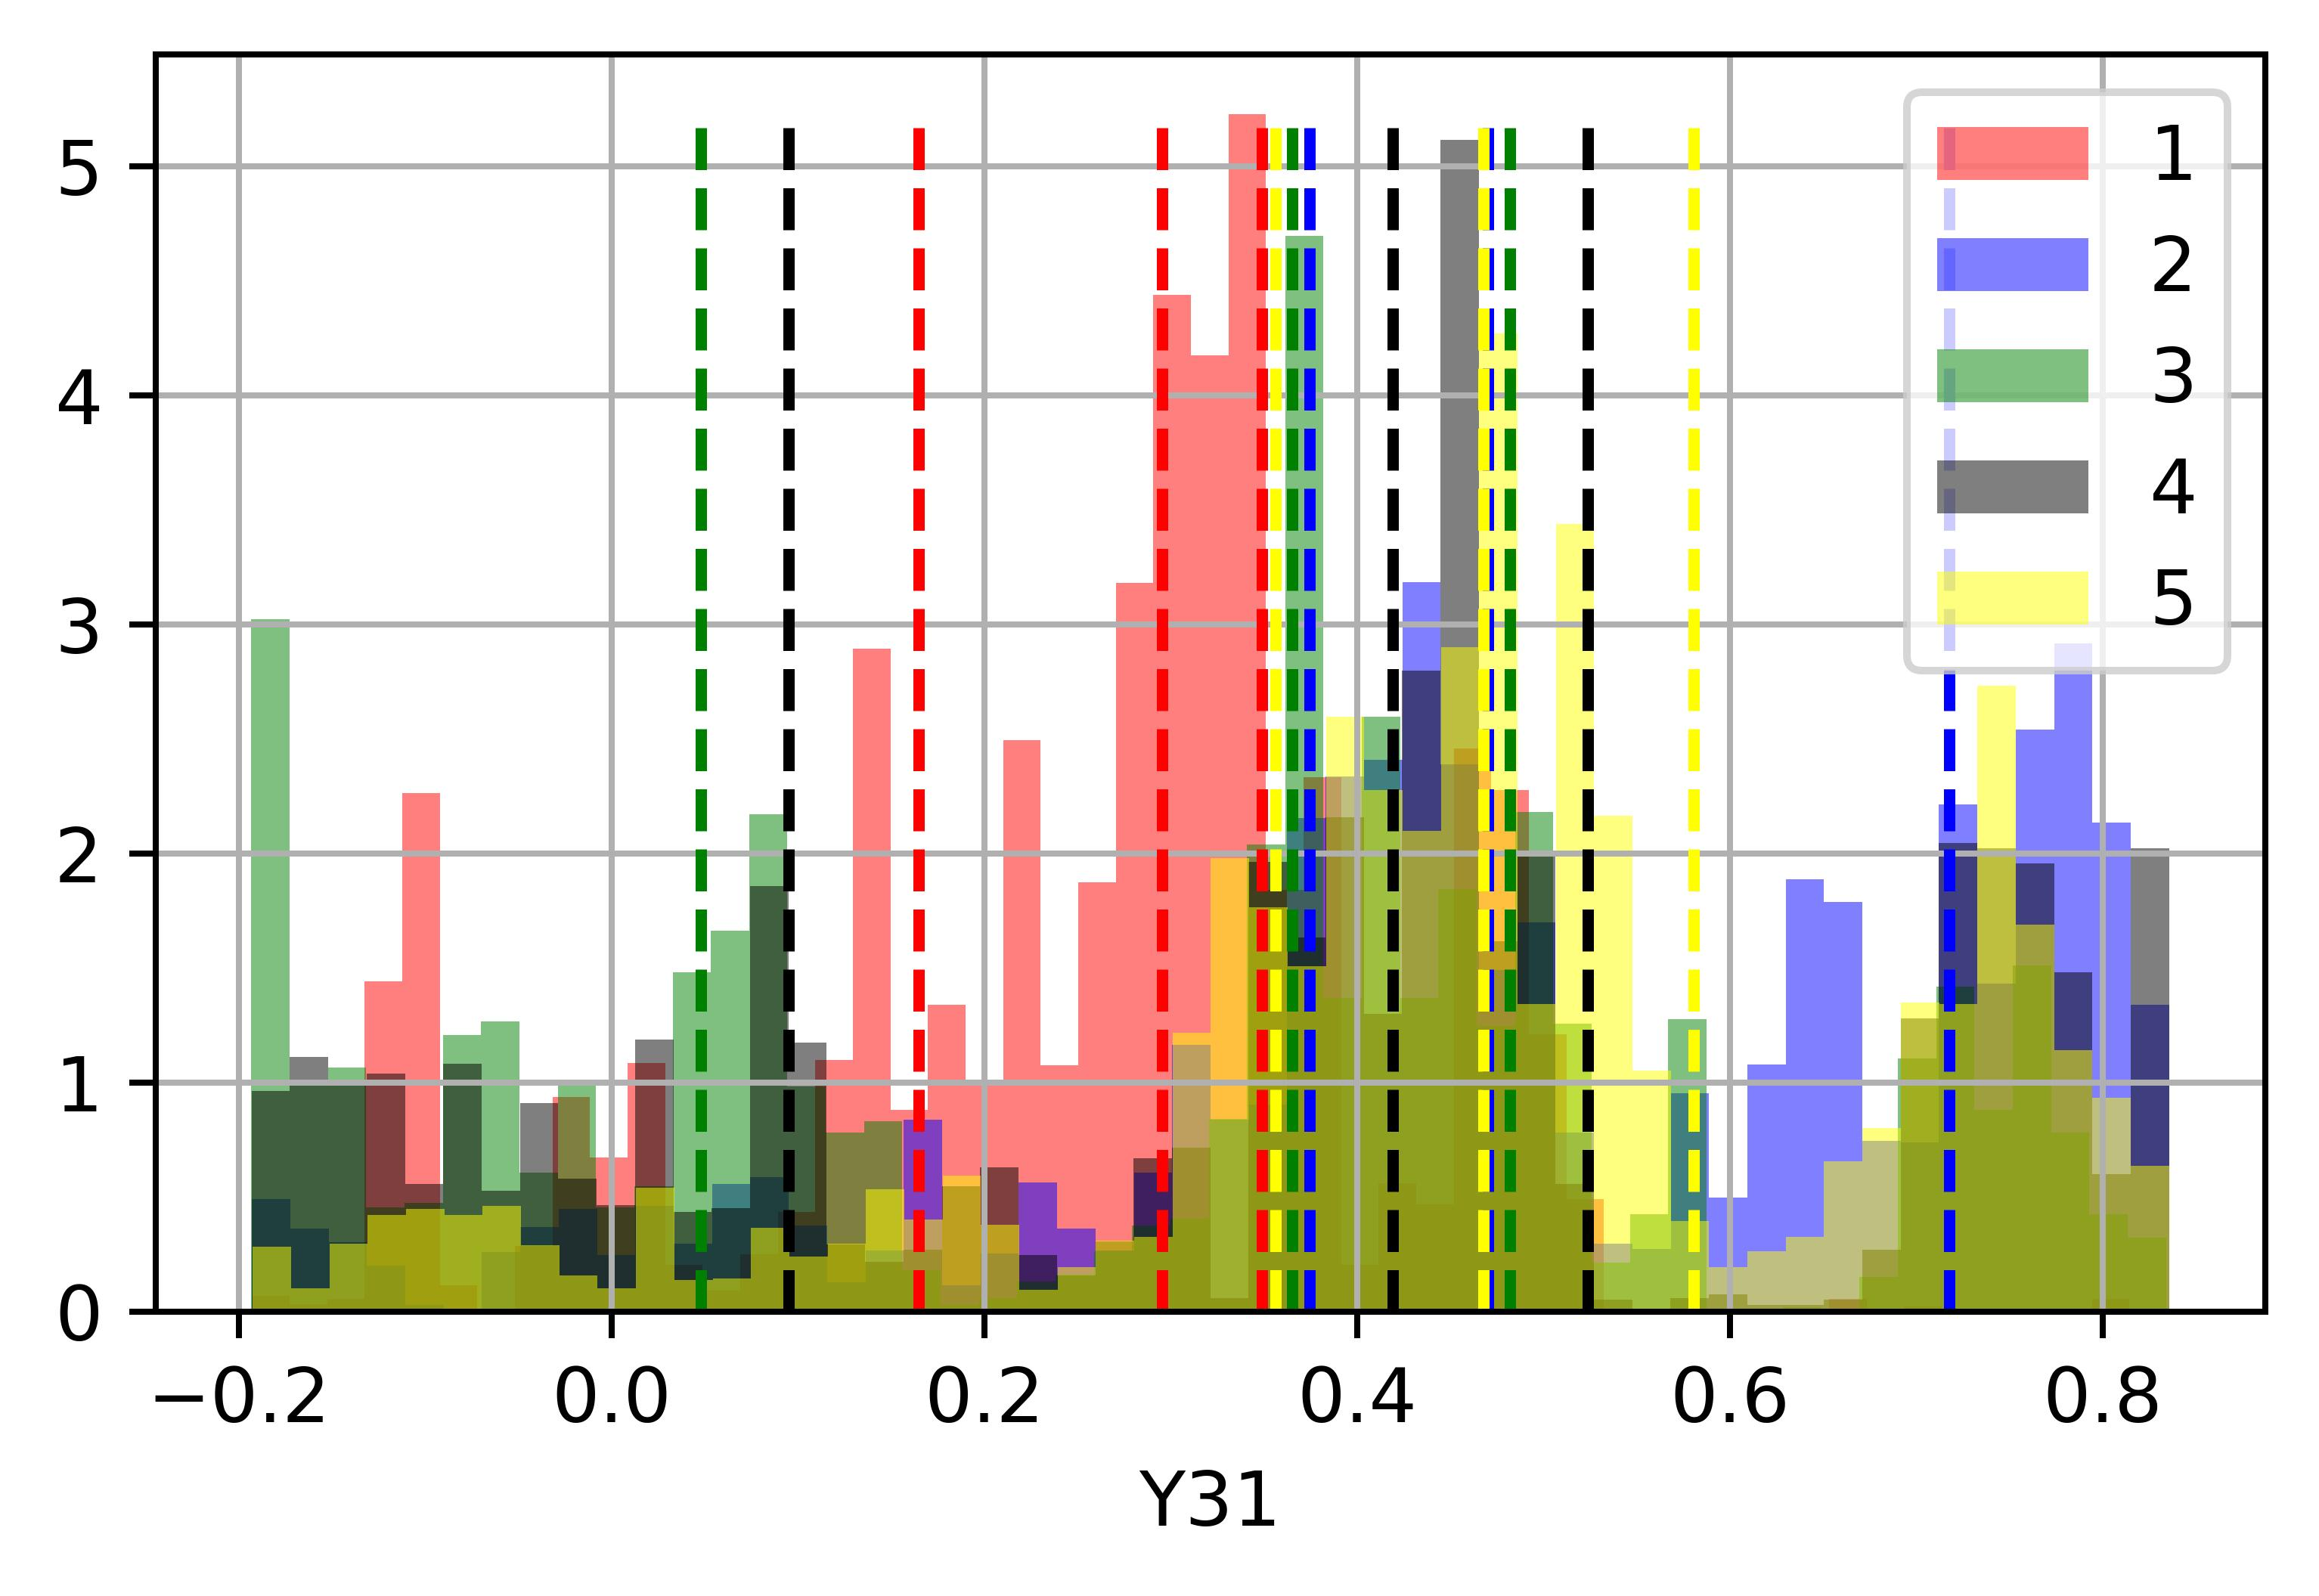
\includegraphics[width=0.18\textwidth]{../code/Task2/Analysis/Hist-Y31}
  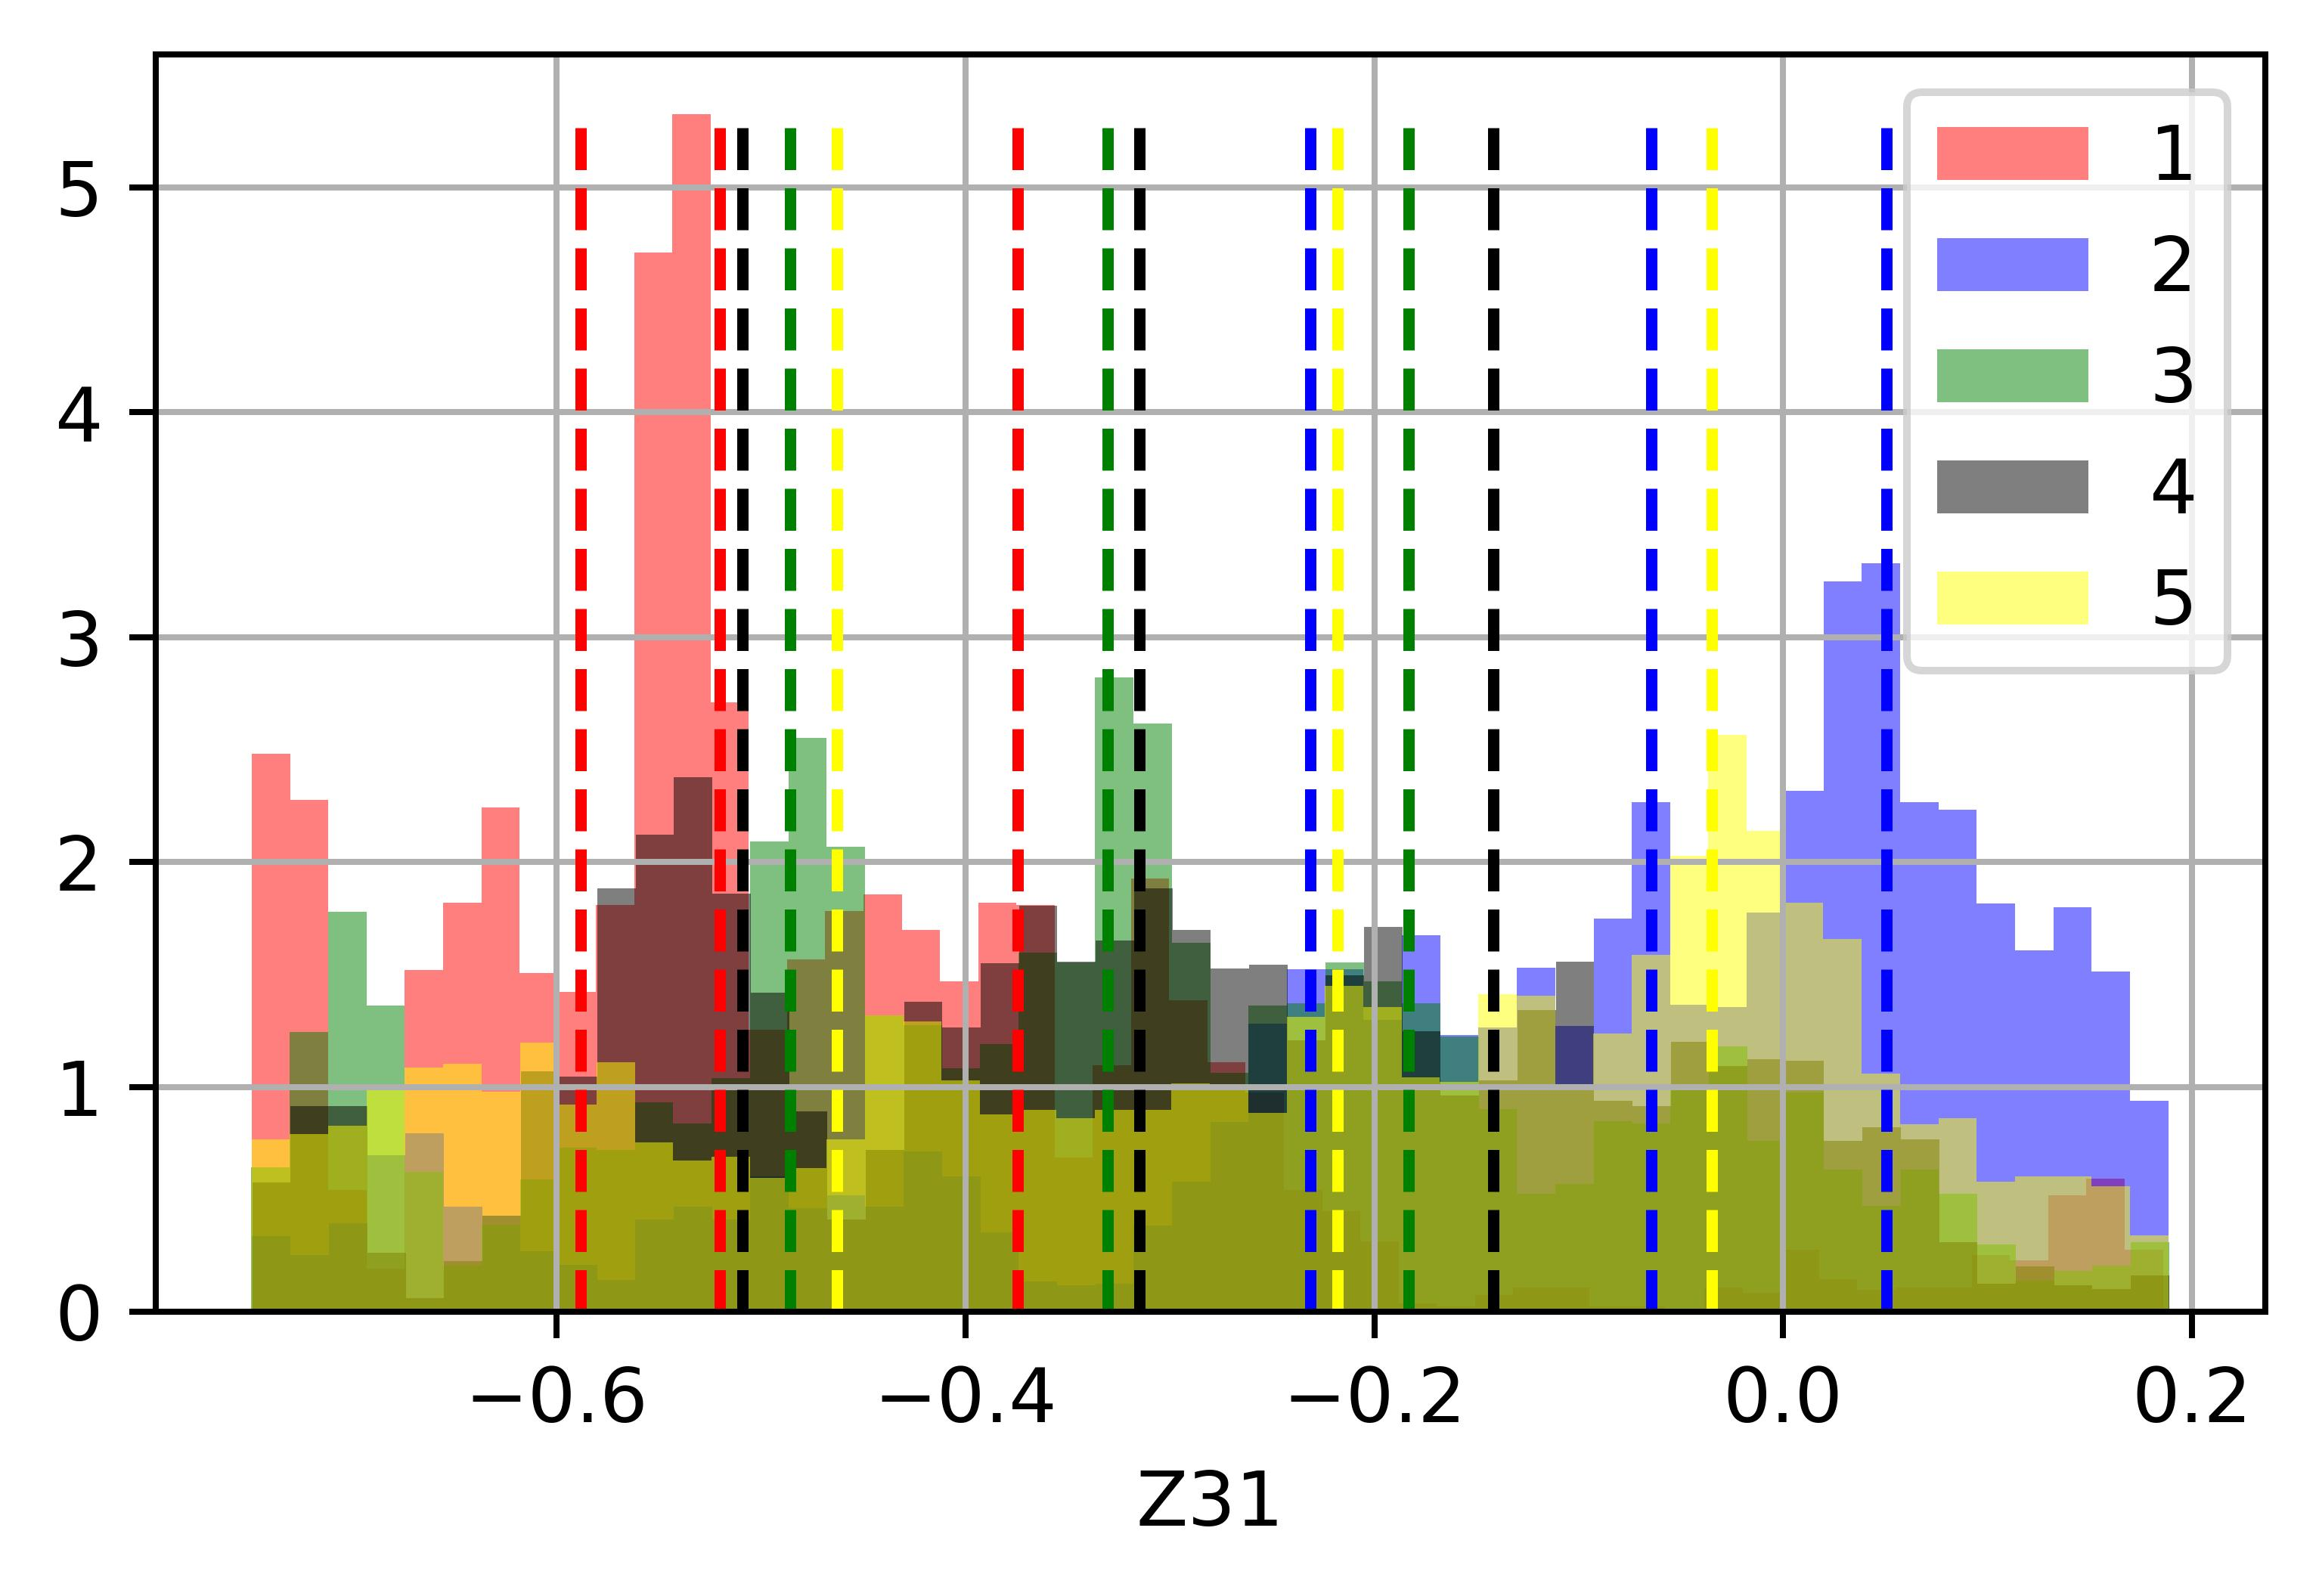
\includegraphics[width=0.18\textwidth]{../code/Task2/Analysis/Hist-Z31}
  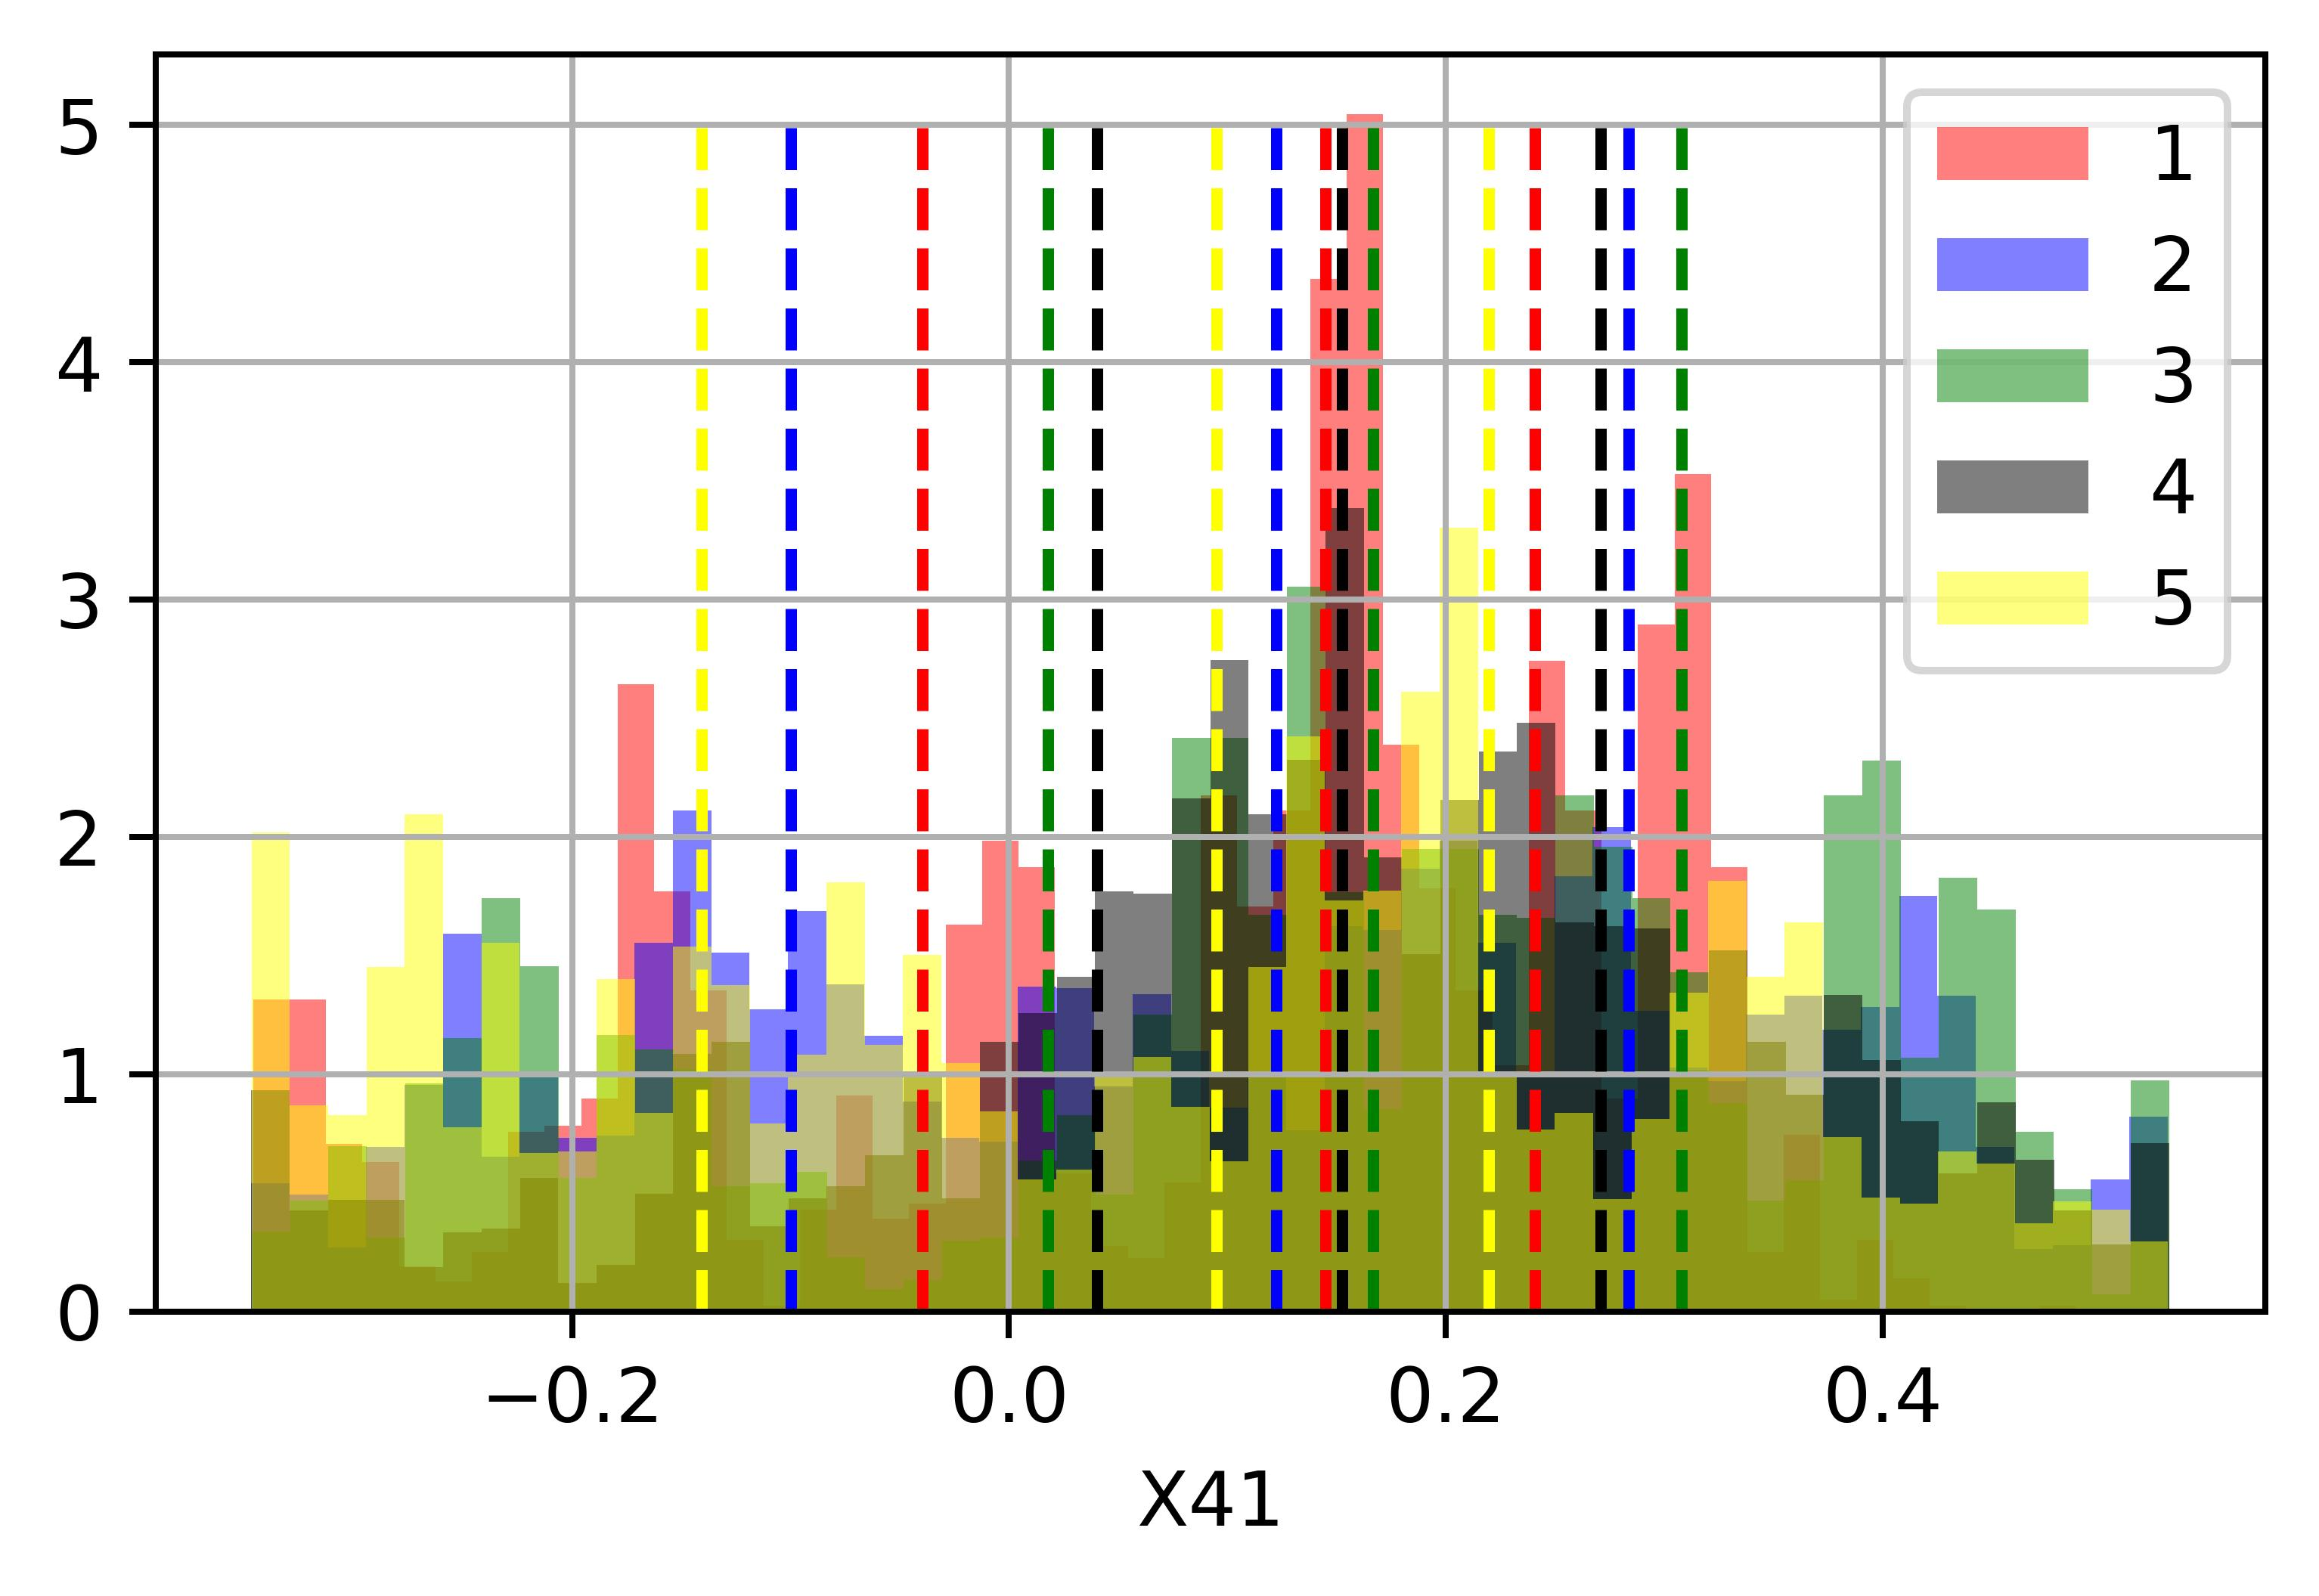
\includegraphics[width=0.18\textwidth]{../code/Task2/Analysis/Hist-X41}
  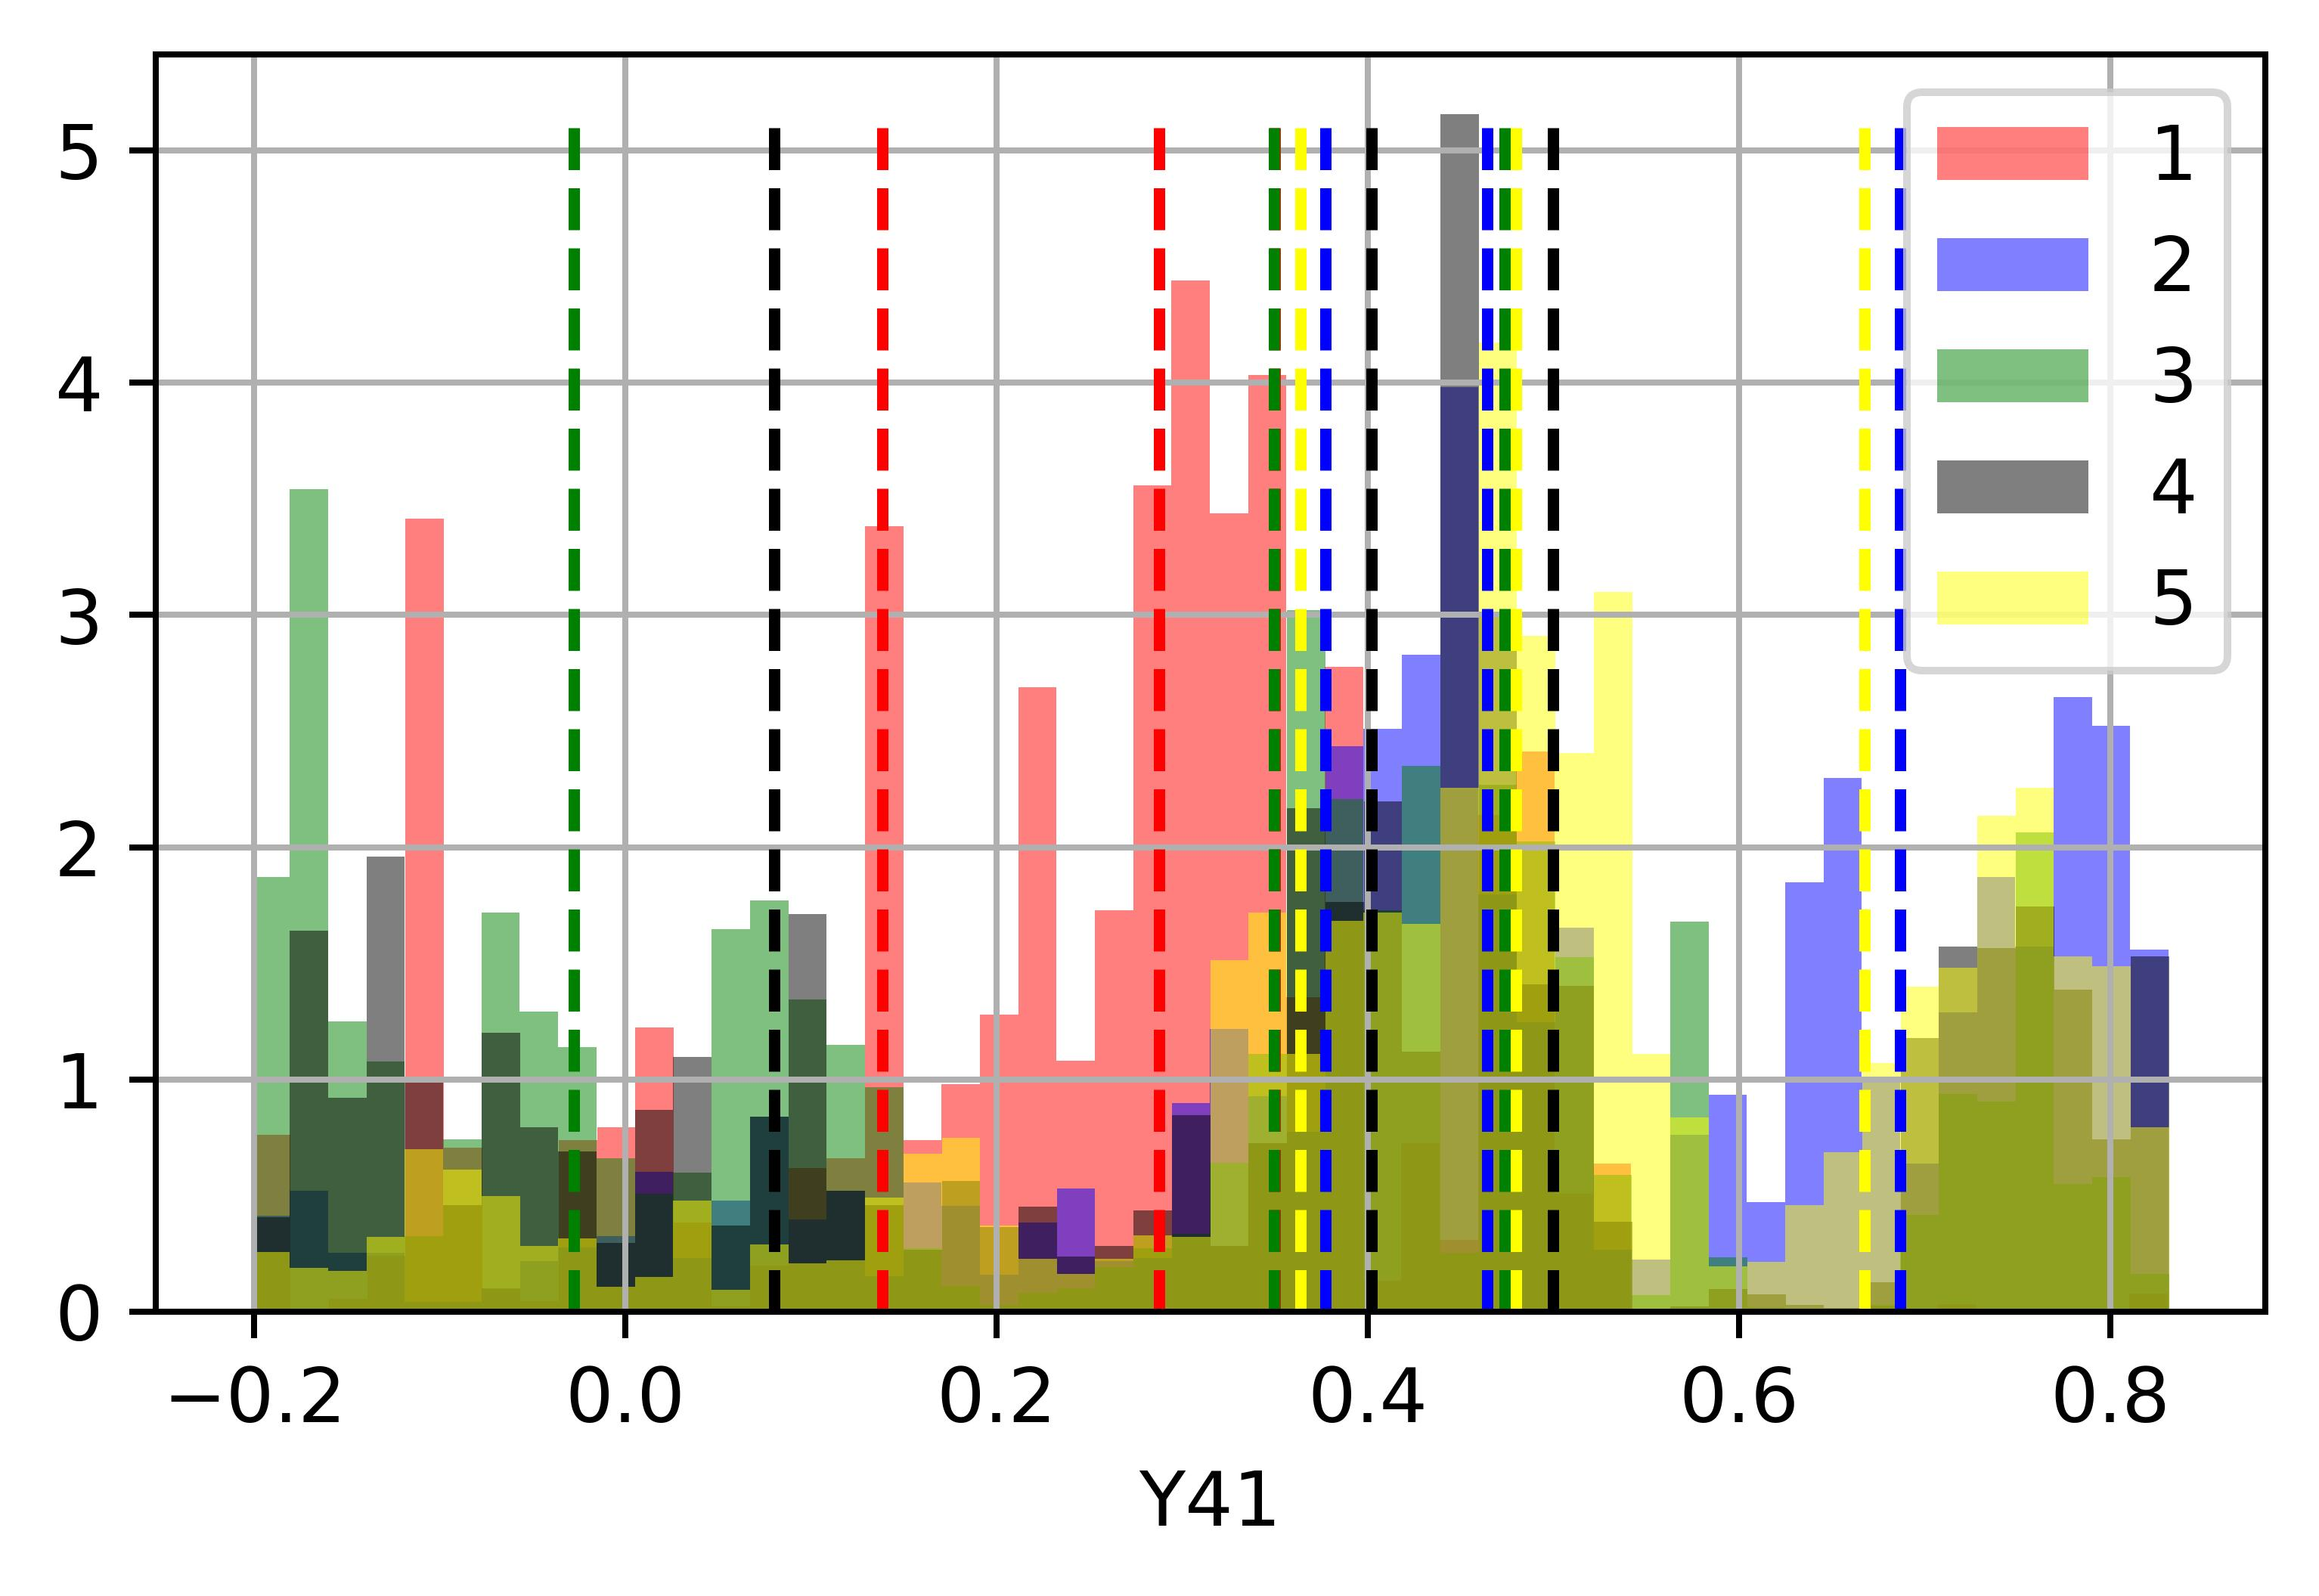
\includegraphics[width=0.18\textwidth]{../code/Task2/Analysis/Hist-Y41}
  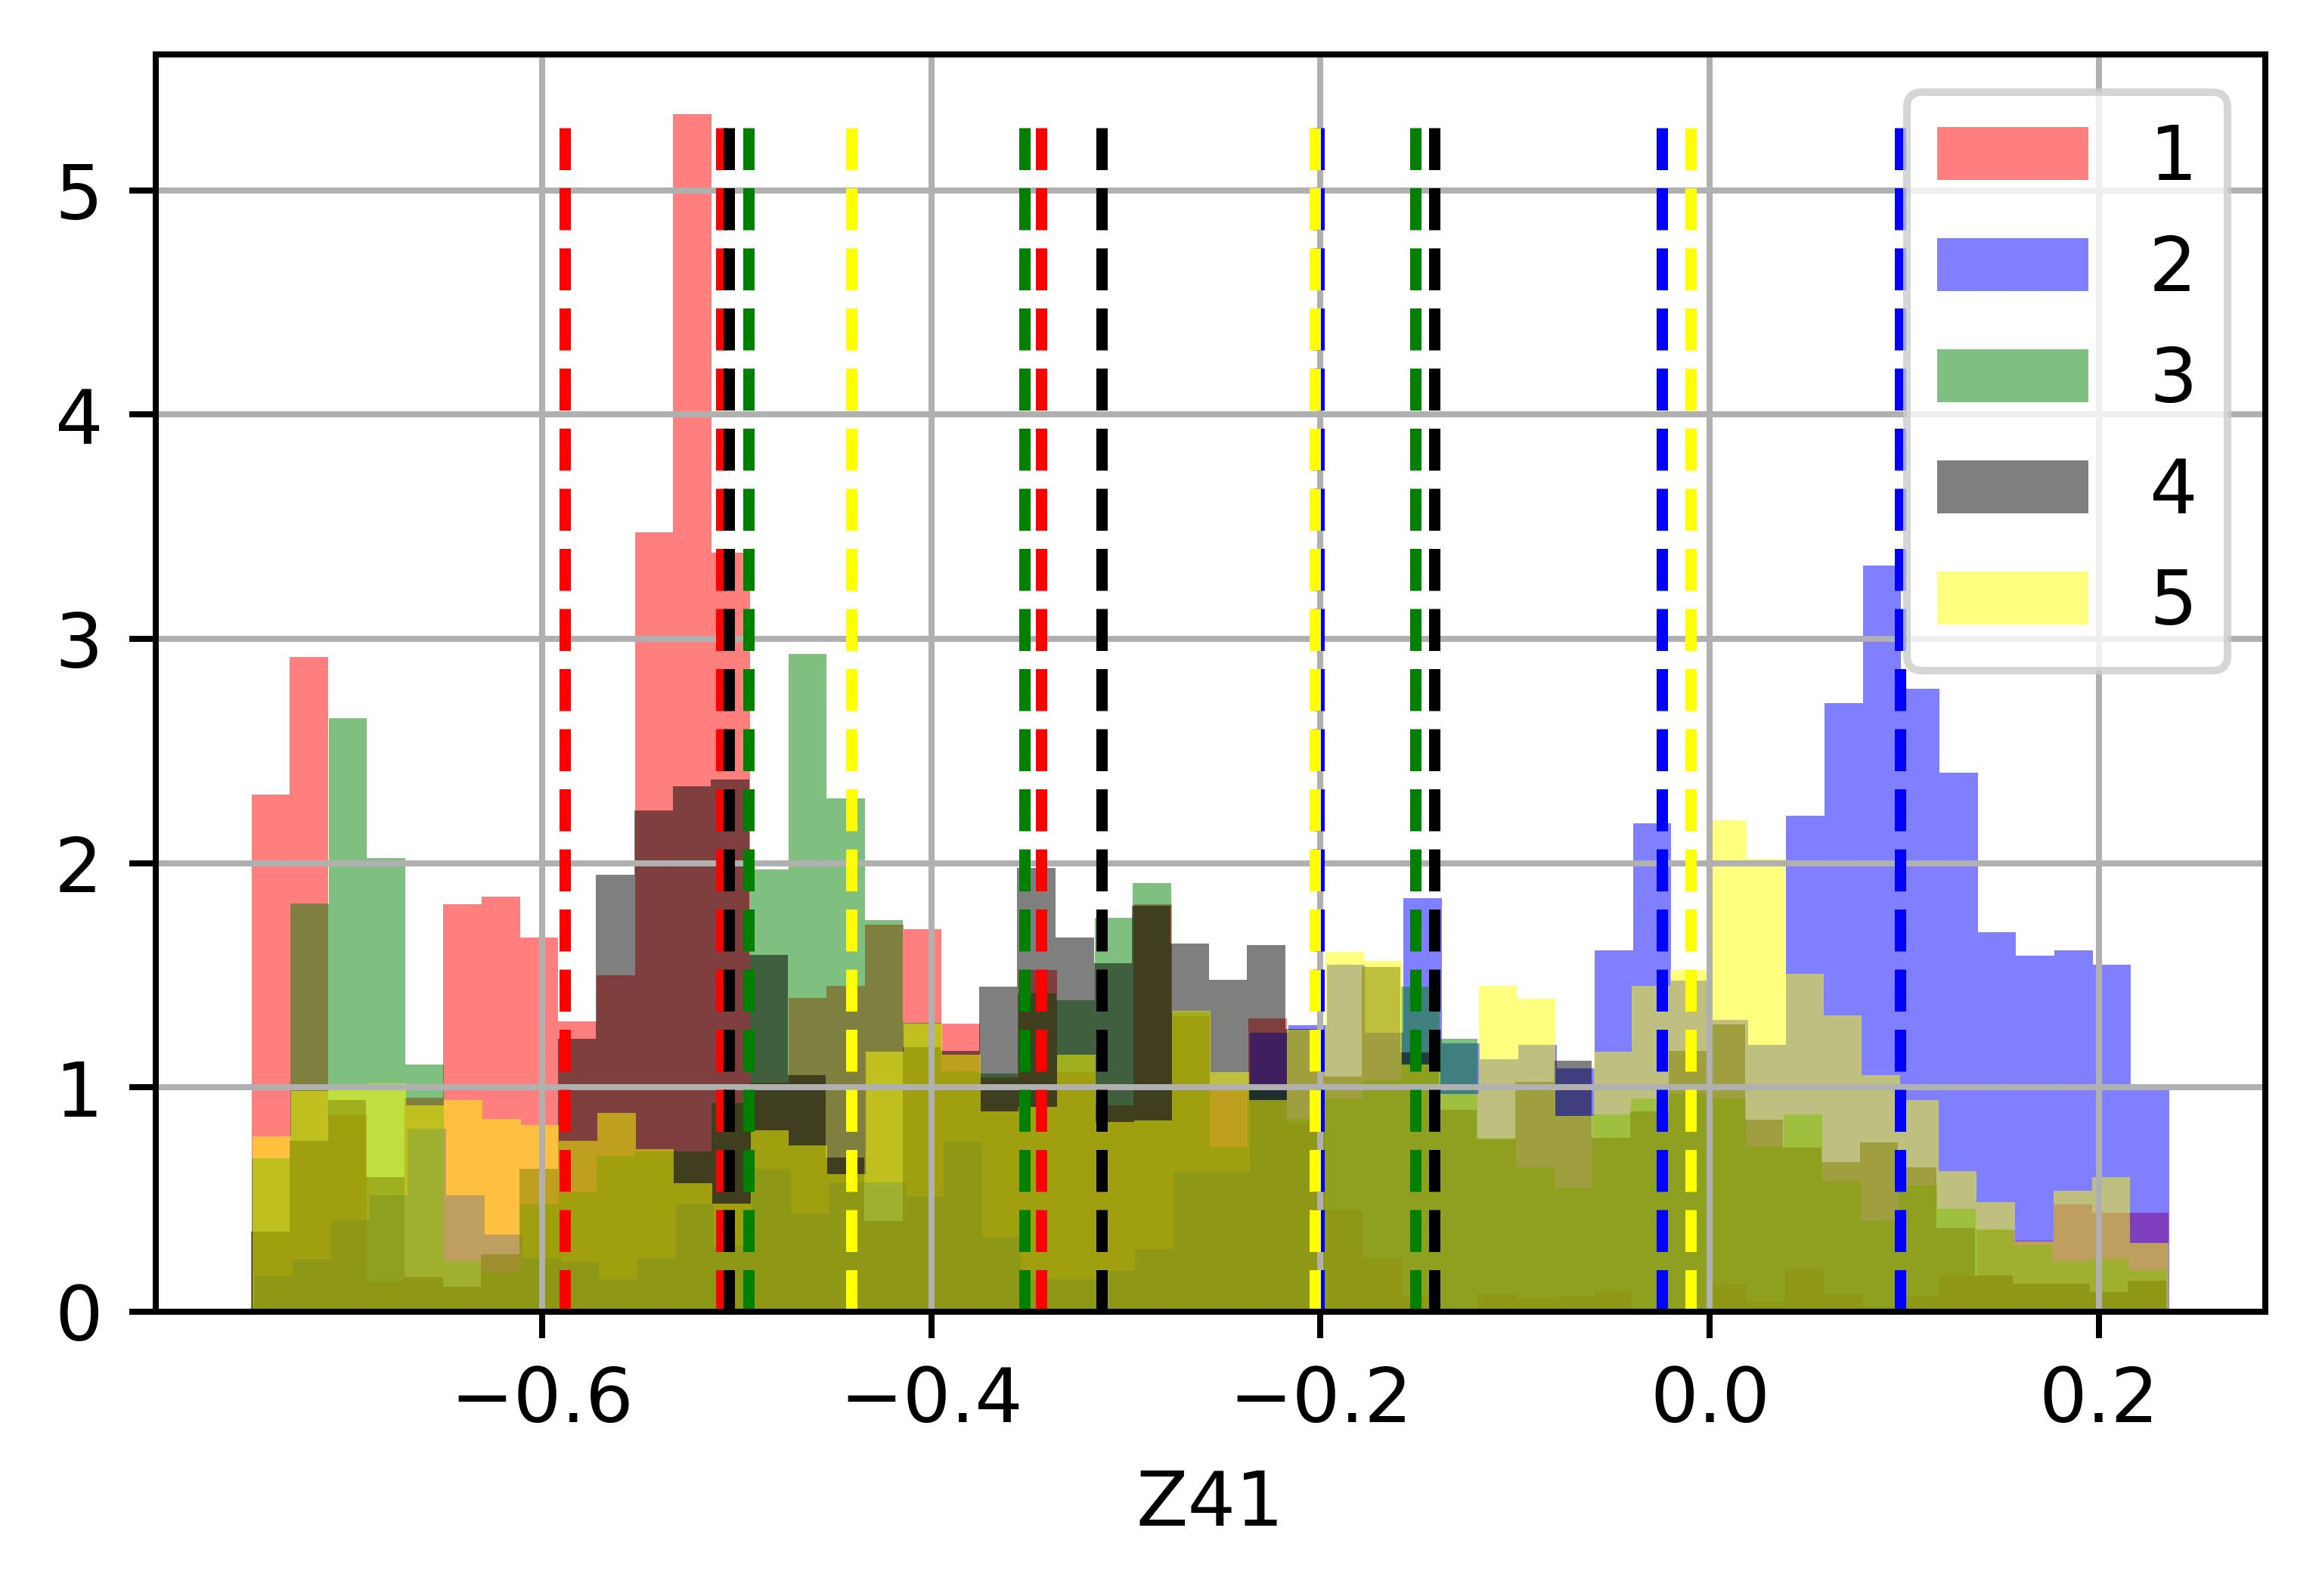
\includegraphics[width=0.18\textwidth]{../code/Task2/Analysis/Hist-Z41} \\
  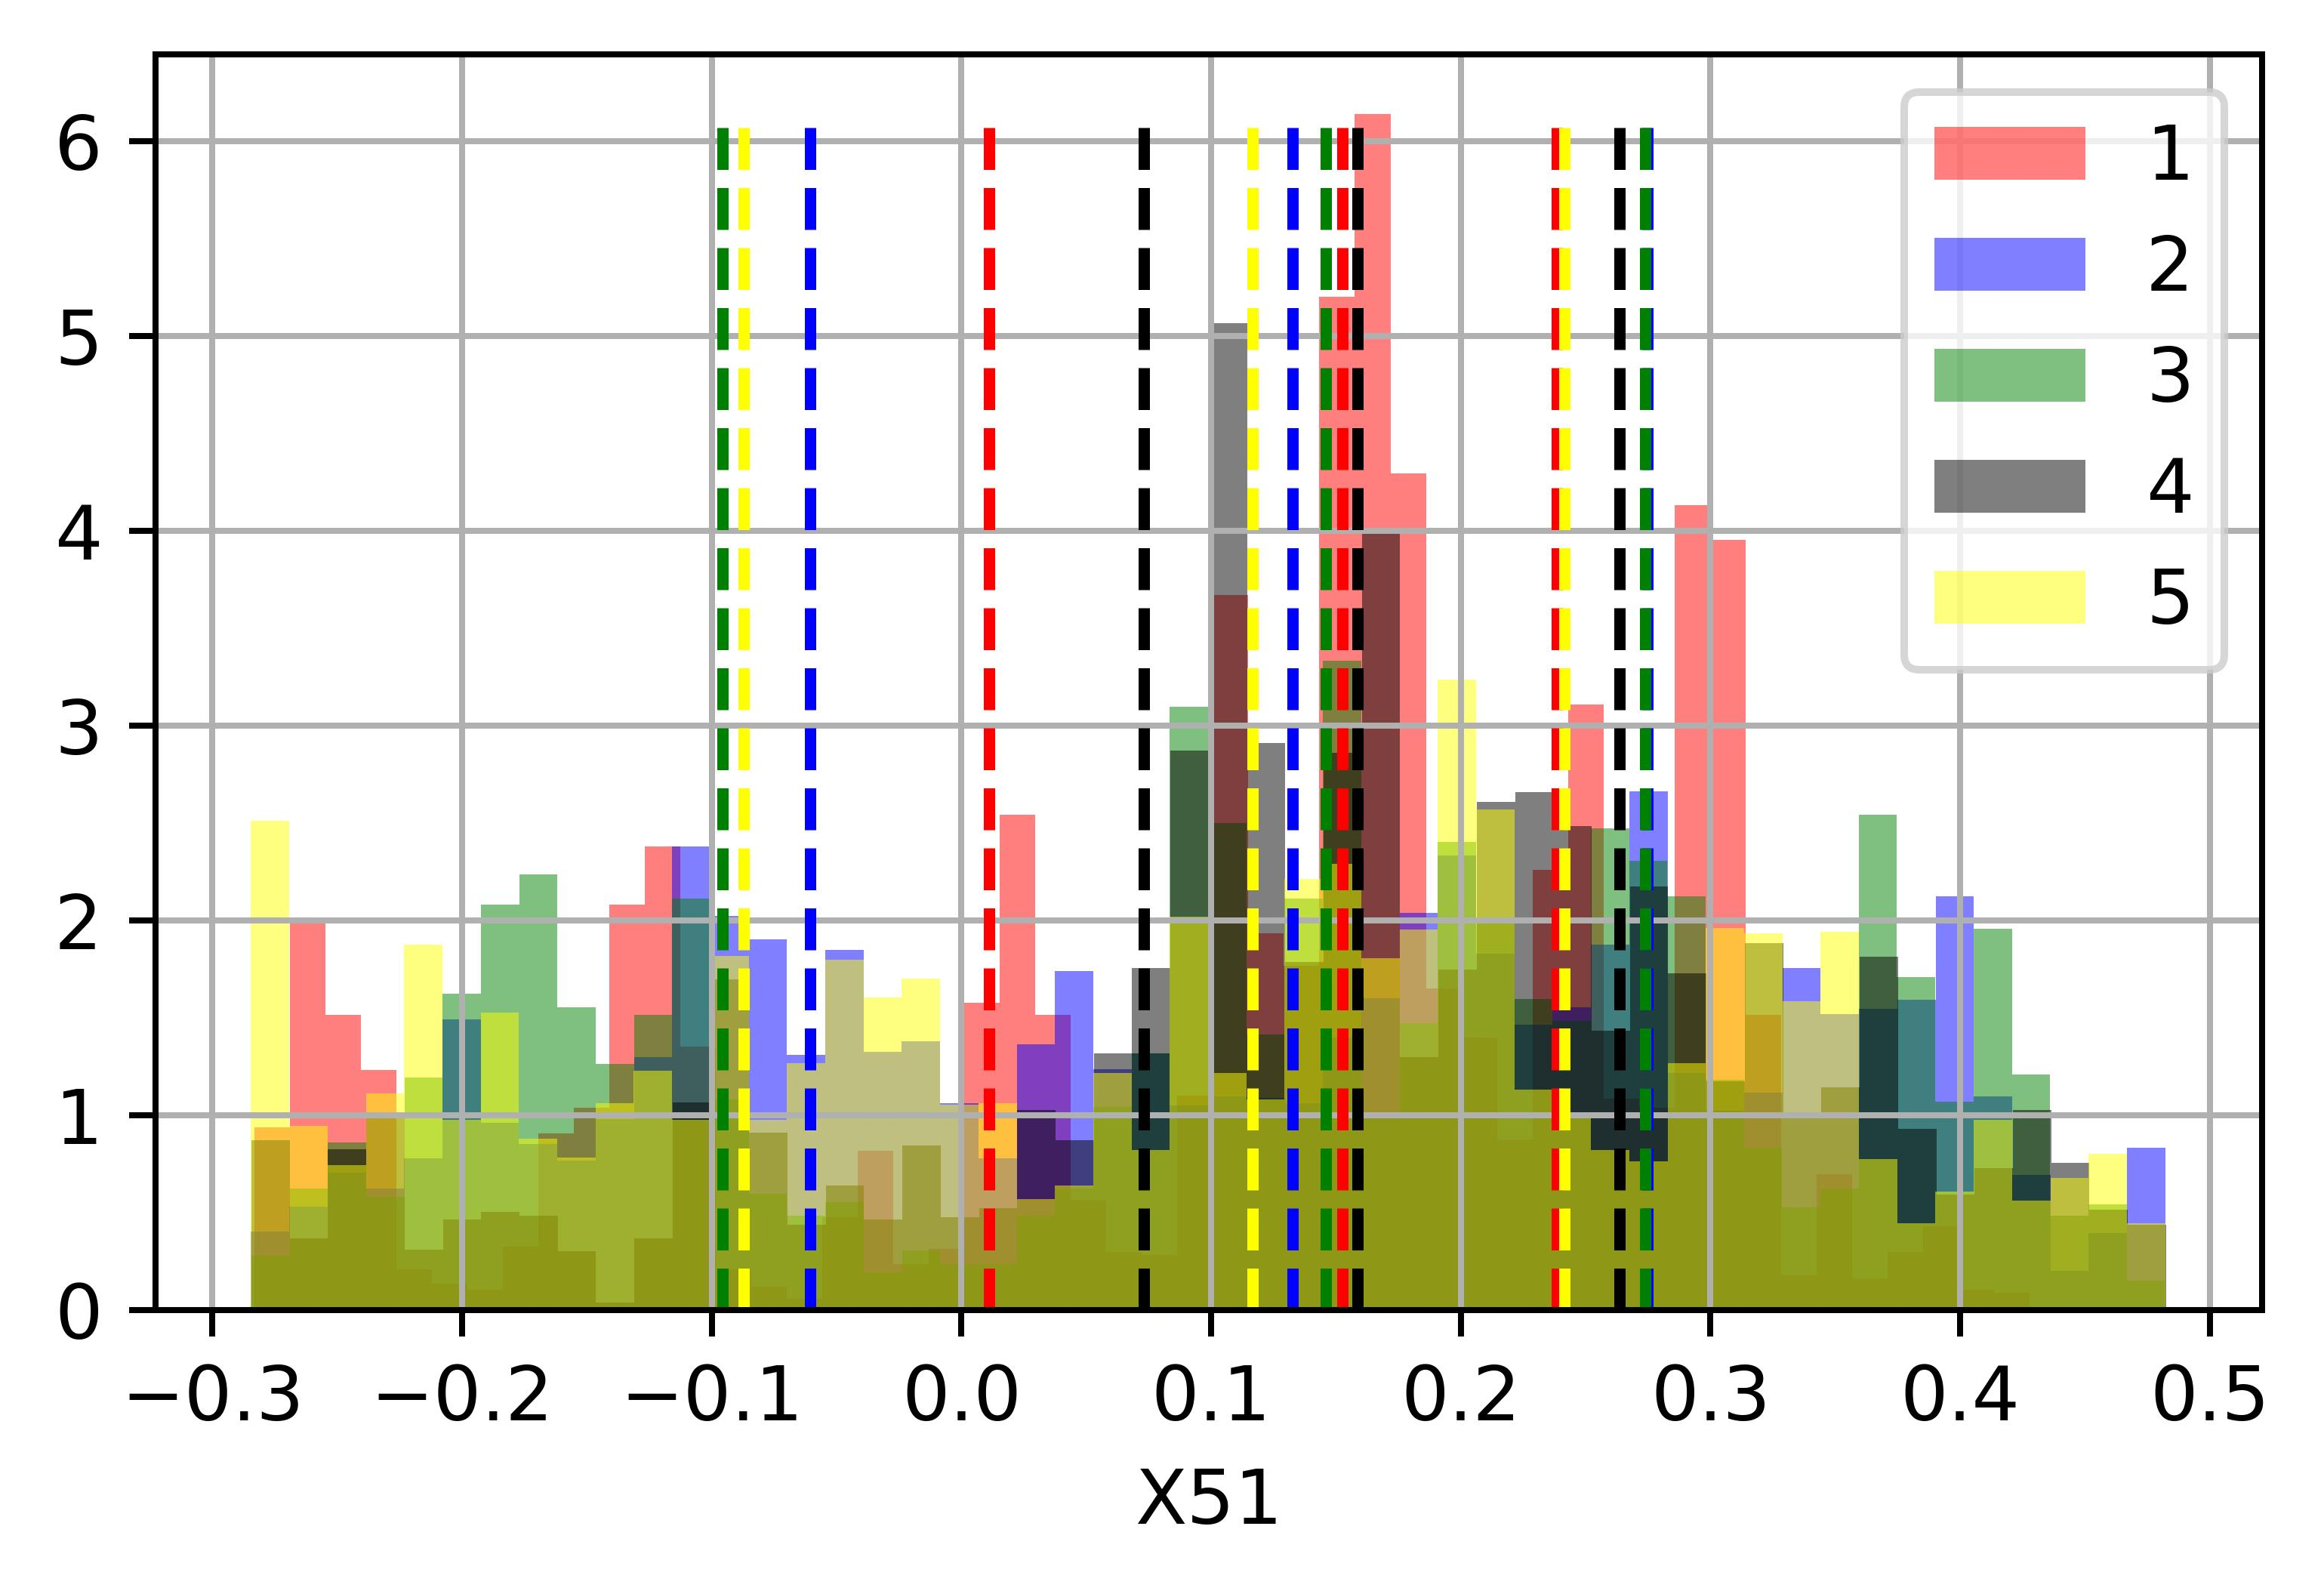
\includegraphics[width=0.18\textwidth]{../code/Task2/Analysis/Hist-X51}
  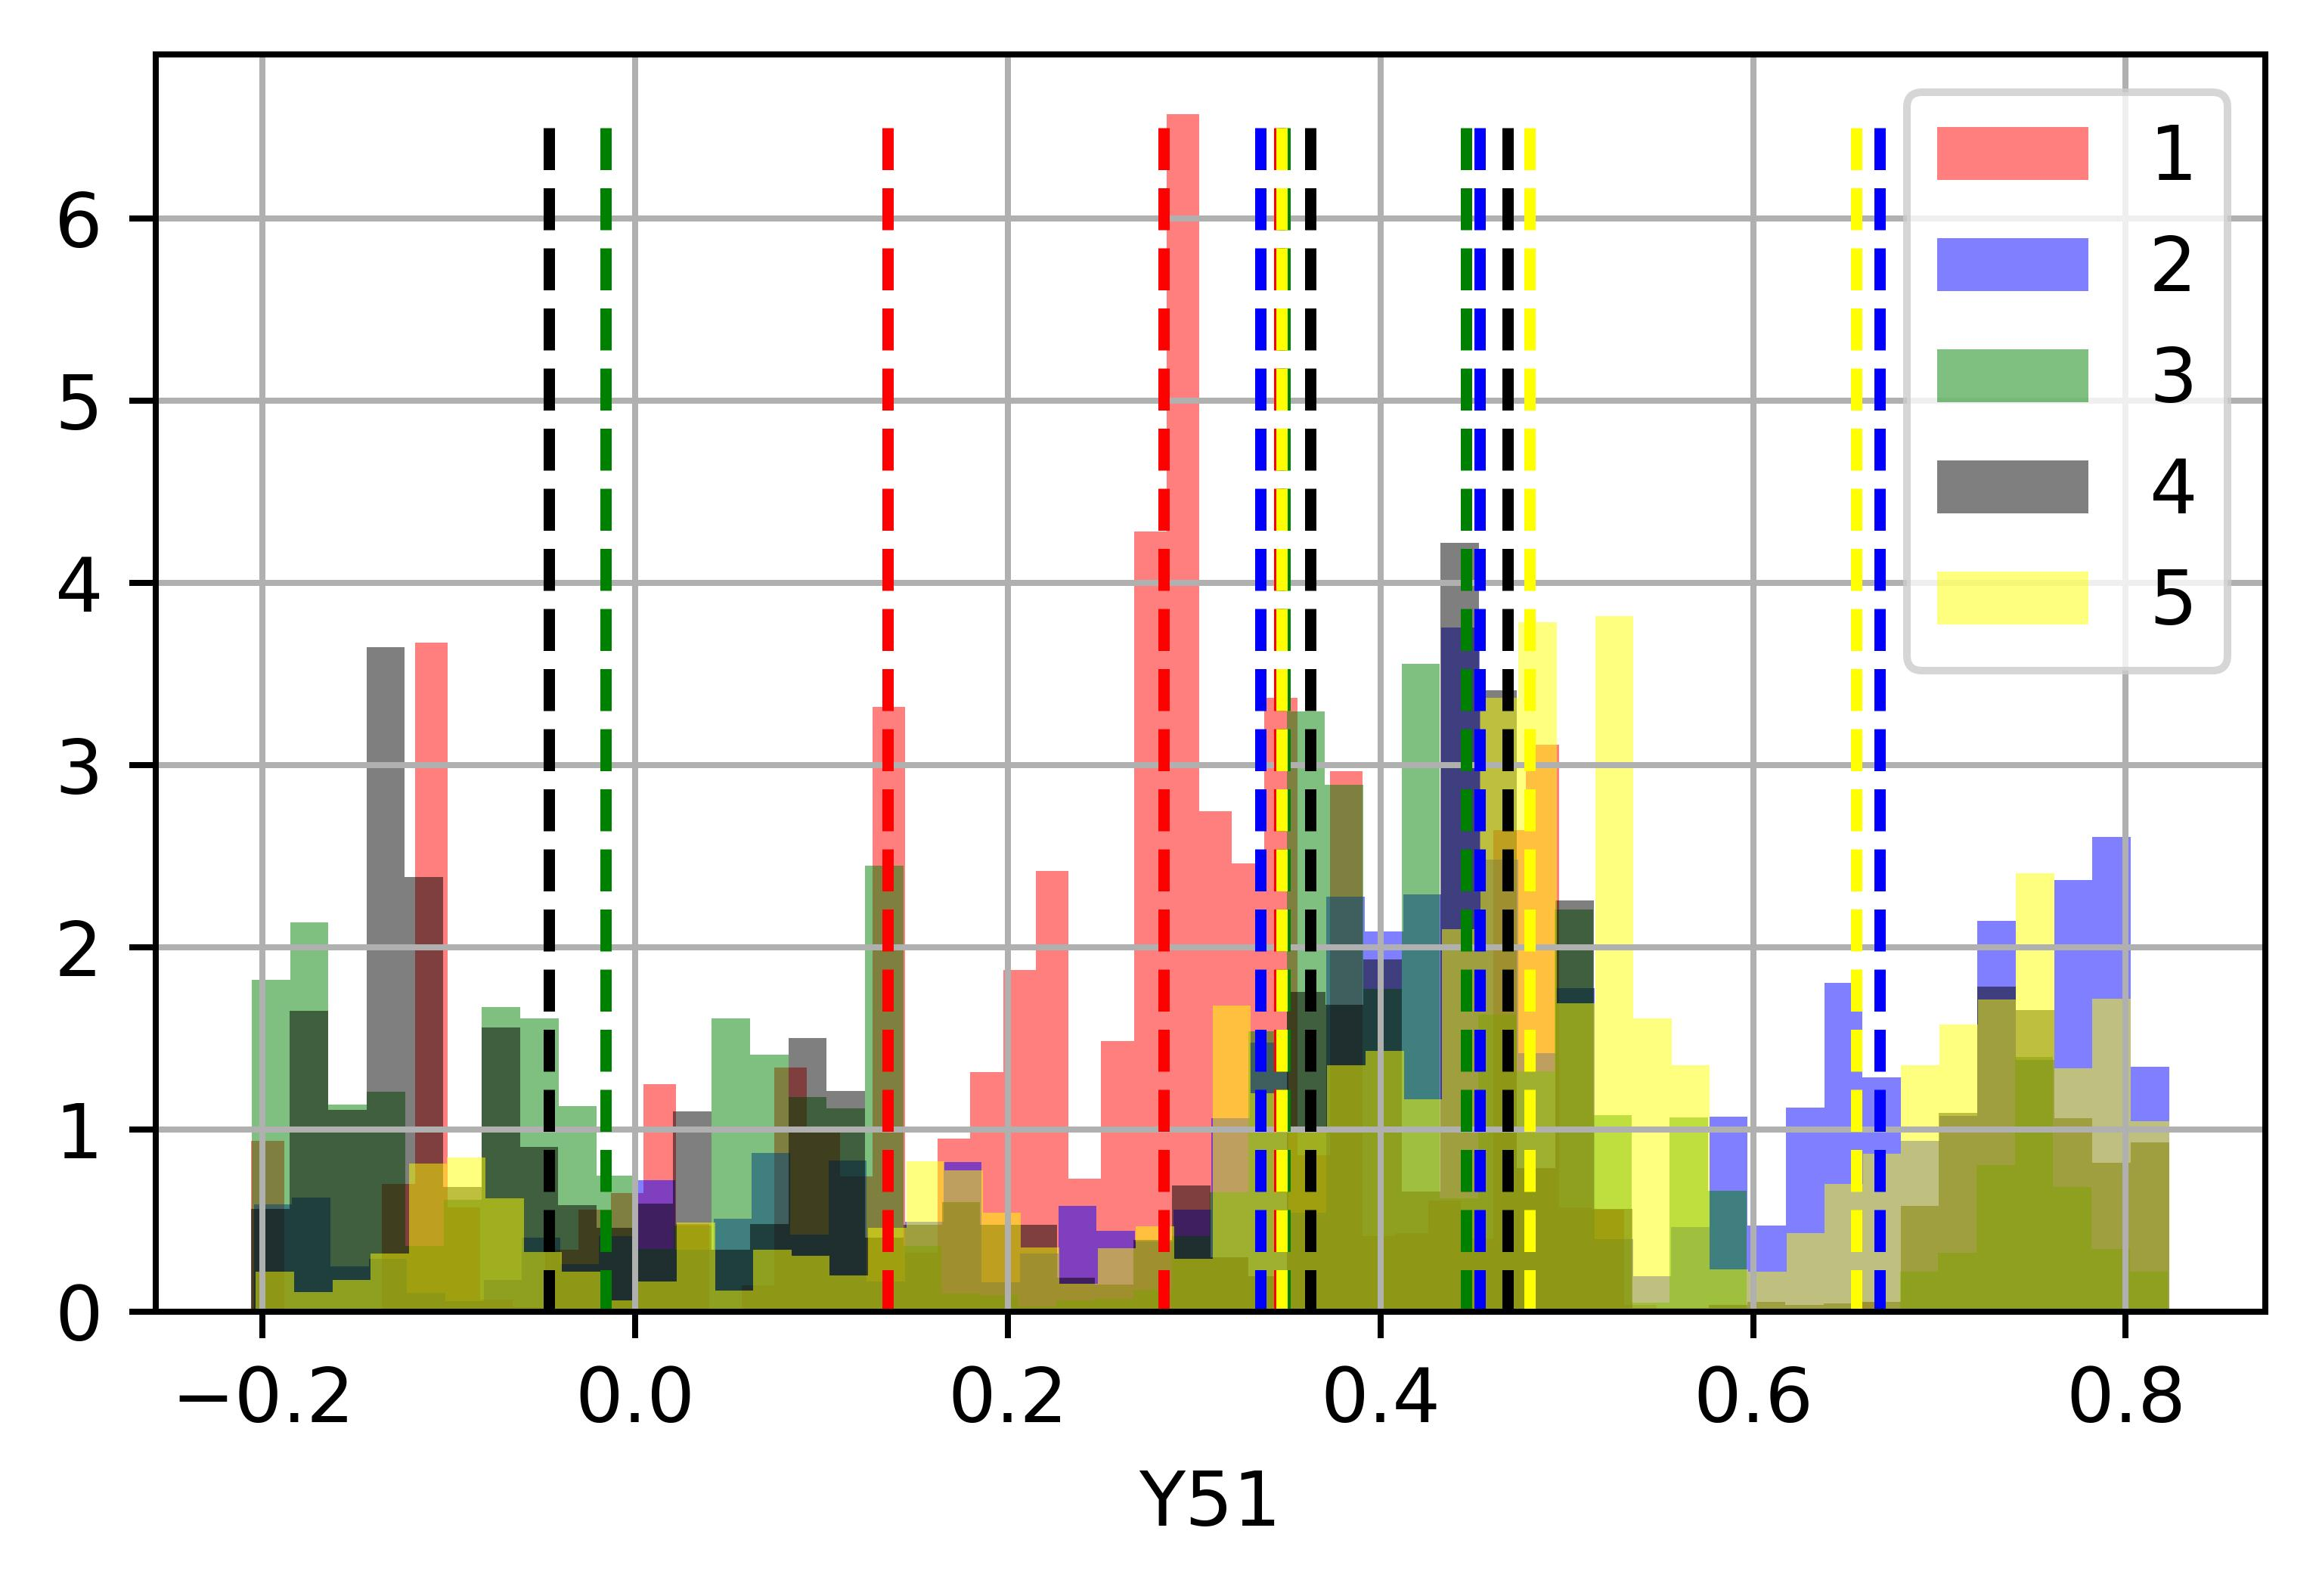
\includegraphics[width=0.18\textwidth]{../code/Task2/Analysis/Hist-Y51}
  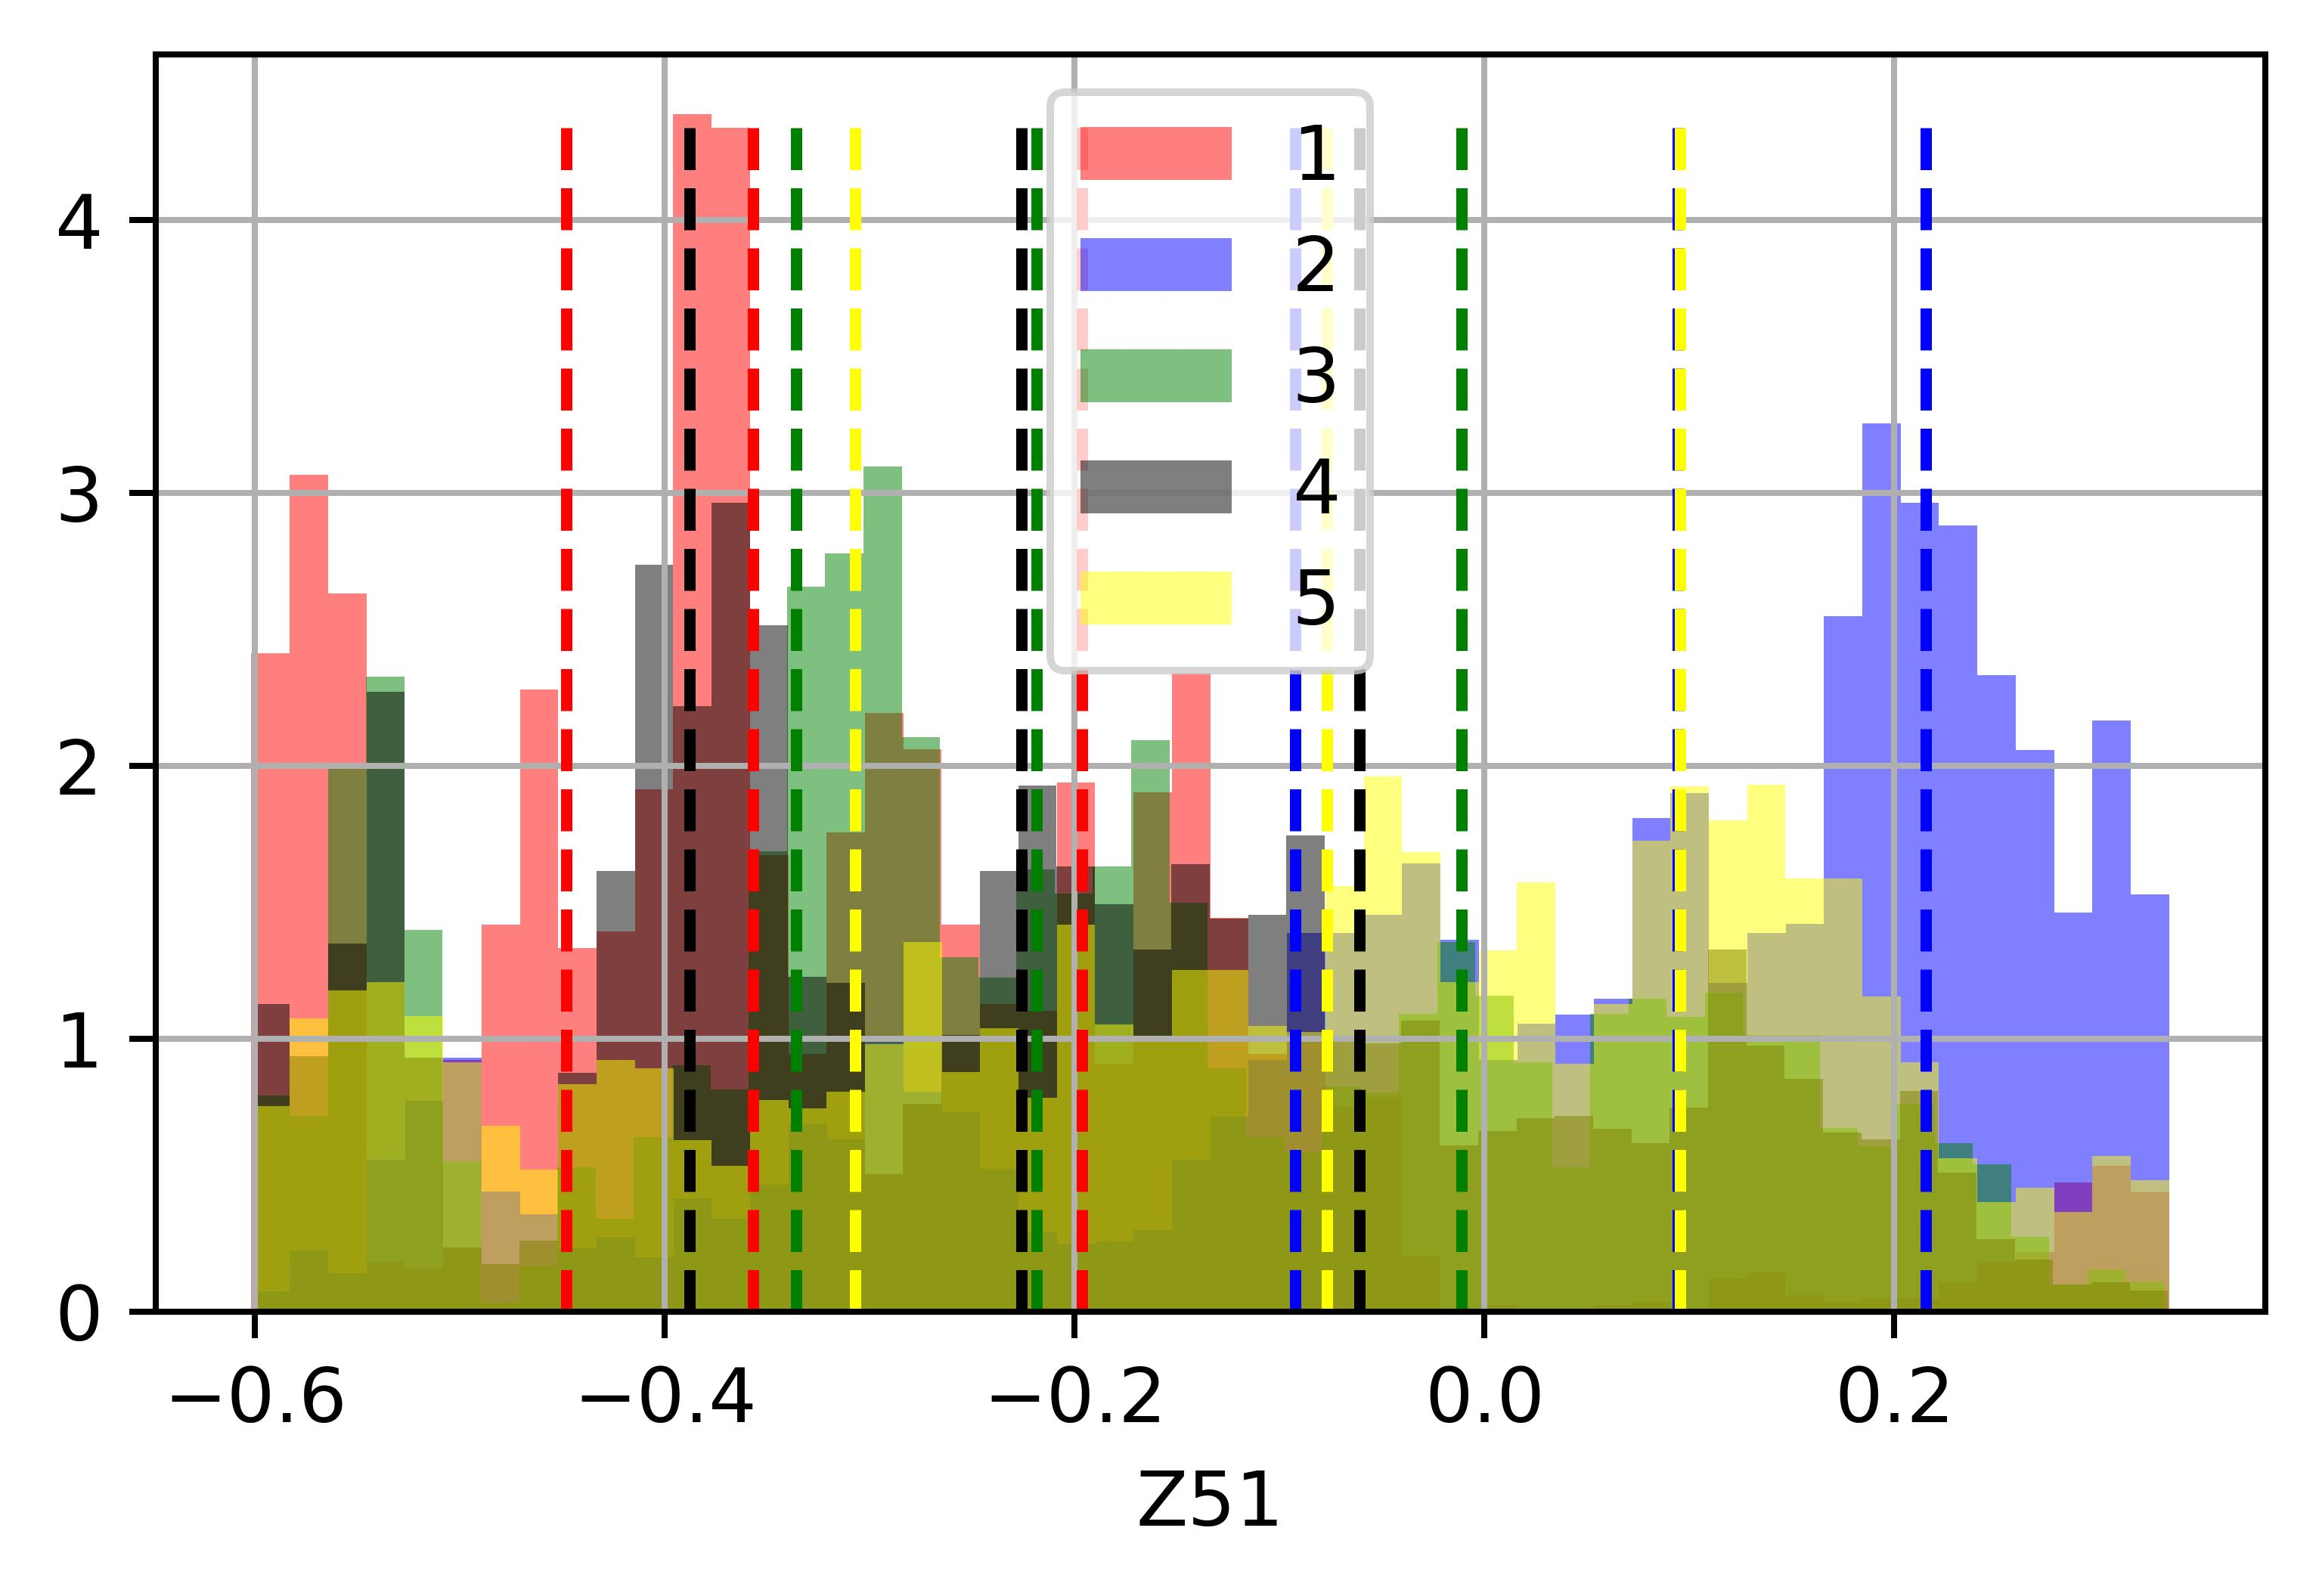
\includegraphics[width=0.18\textwidth]{../code/Task2/Analysis/Hist-Z51}
  \caption{The distribution for each feature (the top and bottom $5\%$ points are considered as outliers, and are not shown). The vertical lines shows the position of first, second and third quartiles.}
  \label{task-2-data-distribution-feature}
\end{figure}

\begin{figure}[H]
  \centering
  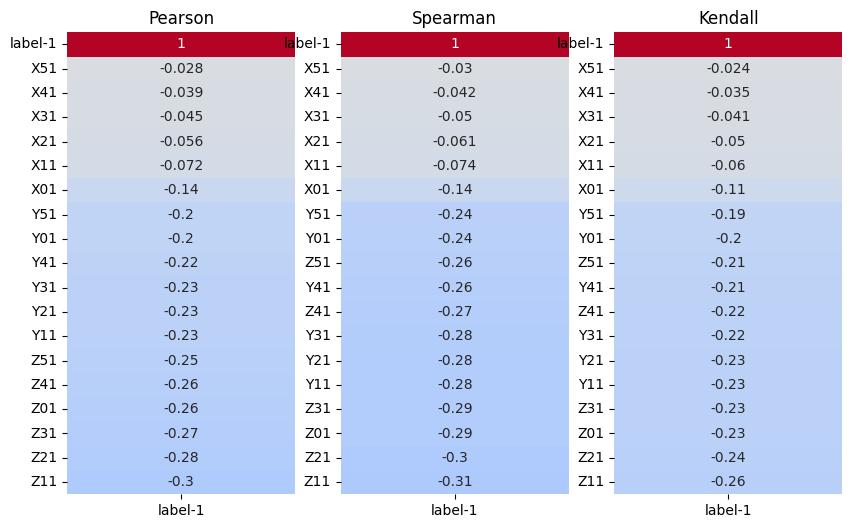
\includegraphics[width=0.45\textwidth]{../code/Task2/Analysis/corrcoef-1.jpg}
  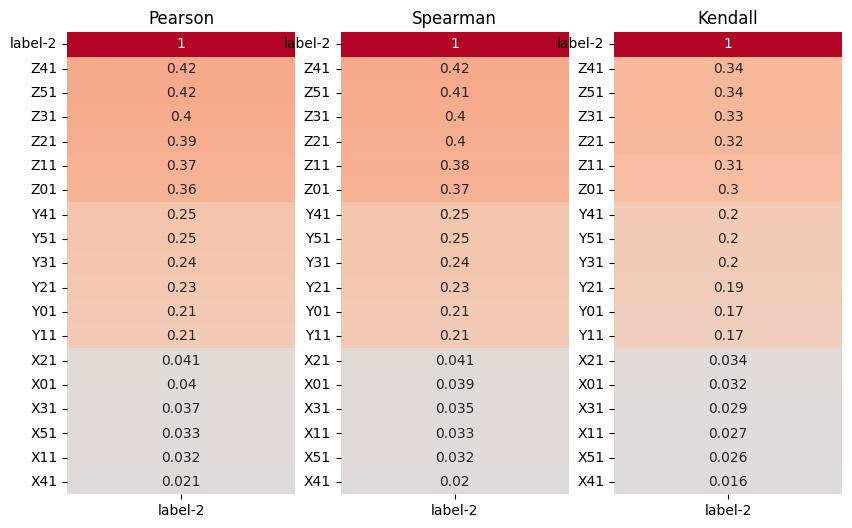
\includegraphics[width=0.45\textwidth]{../code/Task2/Analysis/corrcoef-2.jpg} \\
  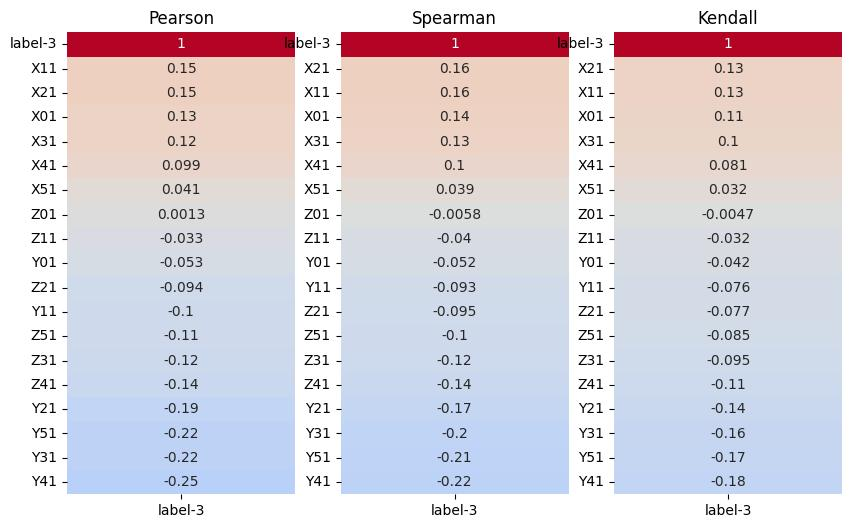
\includegraphics[width=0.45\textwidth]{../code/Task2/Analysis/corrcoef-3.jpg}
  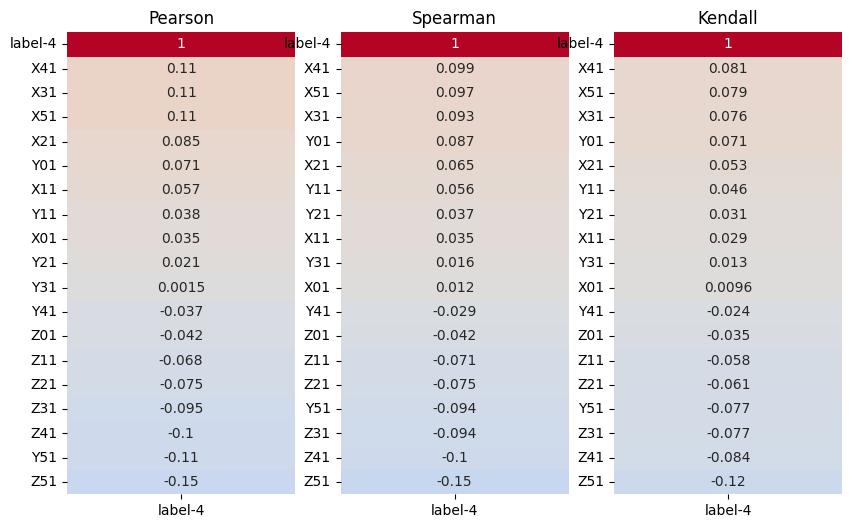
\includegraphics[width=0.45\textwidth]{../code/Task2/Analysis/corrcoef-4.jpg} \\
  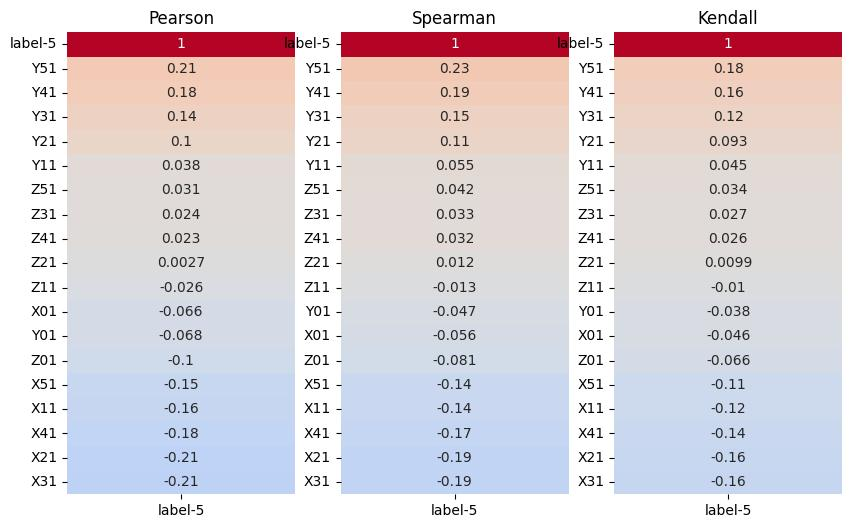
\includegraphics[width=0.45\textwidth]{../code/Task2/Analysis/corrcoef-5.jpg}
  \caption{Correlation coefficient for each features.}
  \label{task-2-correlation-coefficient}
\end{figure}

After the preparing, the decision tree and MLP is applied to the data. The Table \ref{task-2-result-1} and Table \ref{task-2-result-2} shows the results of decision tree and MLP with different hyperparameters. Each test includes $5$ times cross validation ($80\%$ for training set, $20\%$ for training set) and $1$ times that using all data as training set. And the macro f1 score, time and memory cost are recorded.

The result shows that the f1 score by decision tree can only reach $0.80$ to $0.85$, while the MLP can reach more than $0.90$ and up to $0.97$. As for decision tree, comparing the f1 score given by cross validation and the all training data, we can find that the f1 score on training data is much higher, but can still get higher as the max depth increased, which implies that there might be overfitting on some classes, but under fitting for all data. For the MLP, the larger hidden layer size can significantly increase the f1 score, which shows that there are some complex potential relationship between features and labels, this may also be the reason that the decision tree can't get a higher score since it can be regarded as piecewise constant approximation.

\begin{table}[H]
  \centering
  \begin{tabular}{|c|c|c|c|c|c|}
    \hline
    \makecell{Max                                                  \\Depth} & \makecell{Num of                                                          \\ Threshold} & Criterion & \makecell{Feature \\ Selection}& \makecell{F1 Score \\ (Test/Train)} & \makecell{Time/Mem \\ (s/MB)}               \\
    \hline
    $10$ & $64$  & gini    & False & $0.8097/0.8359$ & $153.6/606$ \\
    \hline
    $10$ & $128$ & gini    & False & $0.8043/0.8512$ & $168.5/650$ \\
    \hline
    $12$ & $64$  & gini    & False & $0.8511/0.9106$ & $172.8/601$ \\
    \hline
    $10$ & $64$  & entropy & False & $0.8184/0.8596$ & $147.7/608$ \\
    \hline
    $10$ & $64$  & gini    & True  & $0.8052/0.8334$ & $80.7/585$  \\
    \hline
  \end{tabular}
  \caption{Preformance for decision tree. We tested each option with $5$ times cross validation ($80\%$ for training set, $20\%$ for training set) and $1$ times that using all data as training set. The f1 scores showed in the table is the average f1 score for cross validation and using all data as training set (in this case, we just tested the model on training data) and using all data as training set (in this case, we just tested the model on training data), the time is the total time for $6$ run, and the memory usage is tested using all the data as training set.}
  \label{task-2-result-1}
\end{table}

\begin{table}[H]
  \centering
  \begin{tabular}{|c|c|c|c|c|c|}
    \hline
    Dropout & Hidden Size & \makecell{Feature                                        \\ Selection} &Batch Size & \makecell{F1 Score \\ (Test/Train)} & \makecell{Time/Mem \\ (s/MB)} \\
    \hline
    $0.3$   & $128$       & False             & 512  & $0.9617/0.9718$ & $219.4/856$ \\
    \hline
    $0.3$   & $64$        & False             & 512  & $0.9173/0.9253$ & $212.9/812$ \\
    \hline
    $0.3$   & $256$       & False             & 512  & $0.9767/0.9939$ & $221.7/856$ \\
    \hline
    $0.3$   & $128$       & False             & 1024 & $0.9629/0.9743$ & $148.6/857$ \\
    \hline
    $0.3$   & $128$       & False             & 512  & $0.9644/0.9750$ & $381.4/859$ \\
    \hline
    $0.3$   & $128$       & True              & 512  & $0.9474/0.9559$ & $171.7/848$ \\
    \hline
  \end{tabular}
  \caption{Preformance for MLP. We tested each option with $5$ times cross validation ($80\%$ for training set, $20\%$ for training set) and $1$ times that using all data as training set. The f1 scores showed in the table is the average f1 score for cross validation and using all data as training set (in this case, we just tested the model on training data), the time is the total time for $6$ run, and the memory usage is tested using all the data as training set.}
  \label{task-2-result-2}
\end{table}

\subsection{Task 3}

The Figure \ref{task-3-overview-flowchart} shows the workflow of task 3. During the preparing, we first visualize the data, and analyze the distribution for each features and the whole data. Then the correlation coefficients between label and each features are computed, which give the evidence for feature selection. And next, for each selected features, the dimension raising is applied to help handle the nonlinearity of data. After the preparing, the logistic regression and MLP is implemented and applied to the data, with different hyperparameters to show the effect of them. In the end, the macro f1 score is used to evaluate the model. In the meanwhile, the time and memory cost is also recorded for analysis.

\begin{figure}[H]
  \centering
  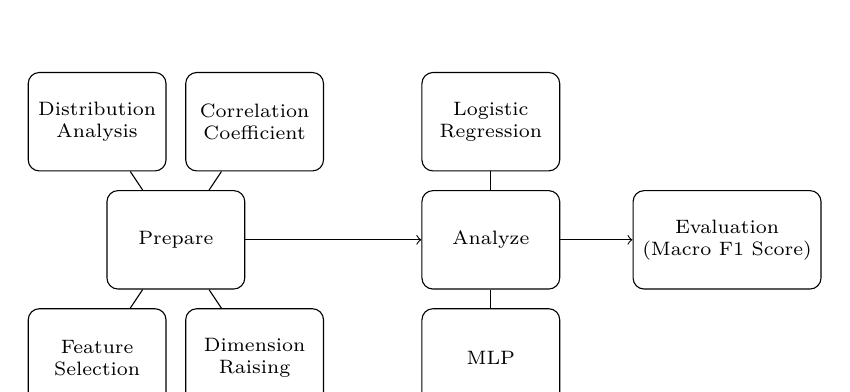
\begin{tikzpicture}[minimum width=1.75cm, minimum height=1.25cm, font=\scriptsize]
    \node[draw, align=center, rounded corners]  (P)   at ( 0,  0.0)    {Prepare};
    \node[draw, align=center, rounded corners]  (D)   at (-1,  1.5)    {Distribution \\ Analysis};
    \node[draw, align=center, rounded corners]  (C)   at ( 1,  1.5)    {Correlation \\ Coefficient};
    \node[draw, align=center, rounded corners]  (F)   at (-1, -1.5)    {Feature \\ Selection};
    \node[draw, align=center, rounded corners]  (R)   at ( 1, -1.5)    {Dimension \\ Raising};

    \node[draw, align=center, rounded corners]  (M)   at ( 4,  0.0)    {Analyze};
    \node[draw, align=center, rounded corners]  (LR)  at ( 4,  1.5)    {Logistic \\ Regression};
    \node[draw, align=center, rounded corners]  (MLP) at ( 4, -1.5)    {MLP};

    \node[draw, align=center, rounded corners]  (E)   at ( 7,  0.0)    {Evaluation \\ (Macro F1 Score)};

    \draw[->] (P) -- (M);

    \draw[-]  (P) -- (D);
    \draw[-]  (P) -- (C);
    \draw[-]  (P) -- (F);
    \draw[-]  (P) -- (R);

    \draw[-]  (M) -- (LR);
    \draw[-]  (M) -- (MLP);

    \draw[->] (M) -- (E);
  \end{tikzpicture}
  \caption{Overview flowchart for task 3.}
  \label{task-3-overview-flowchart}
\end{figure}

The Figure \ref{task-3-data-distribution} is the parallel coordinate plot for each features, where the $10\%$ of total data is chosen. The Figure \ref{task-3-data-distribution-feature} shows the distribution of each feature, where the top and bottom $5\%$ points are considered as outliers, which are not shown in the figure, but still used in training model. And the vertical lines shows the position of first, second and third quartiles. And the Figure \ref{task-3-correlation-coefficient} shows the correlation coefficient between the label and each features.

From These three figures, we can easly see that some features (e.g. V4, V11, V12 and V14) are linear separatable with the absolute value of every correlation coefficients more than $0.6$, implies that these features are highly highly relevant to the label, and can be directly used in the predicting model. In the meanwhile, some features (e.g. V15, V22 and Amount) are totally in a mess, and the absolute value of correlation coefficients are all less then $0.1$, which needed to be deleted in feature selection. As for the rest, the correlation coefficients mostly between $0.2$ and $0.6$ can lead to a weak relationships, and we assume that there might be some potential nonlinear relationship that can be handeled via dimension raising and nonlinear classifiers.

In our implementation, we set the $0.1$ as the threshold and only the features with correlation coefficients great than $0.1$ or less than $-0.1$ will be selected. And the degree of dimension raising is not higher than $3$ due to the high degree polynomial features might cause numerical instability or be correlated, which can making optimization more difficult.

\begin{figure}[H]
  \centering
  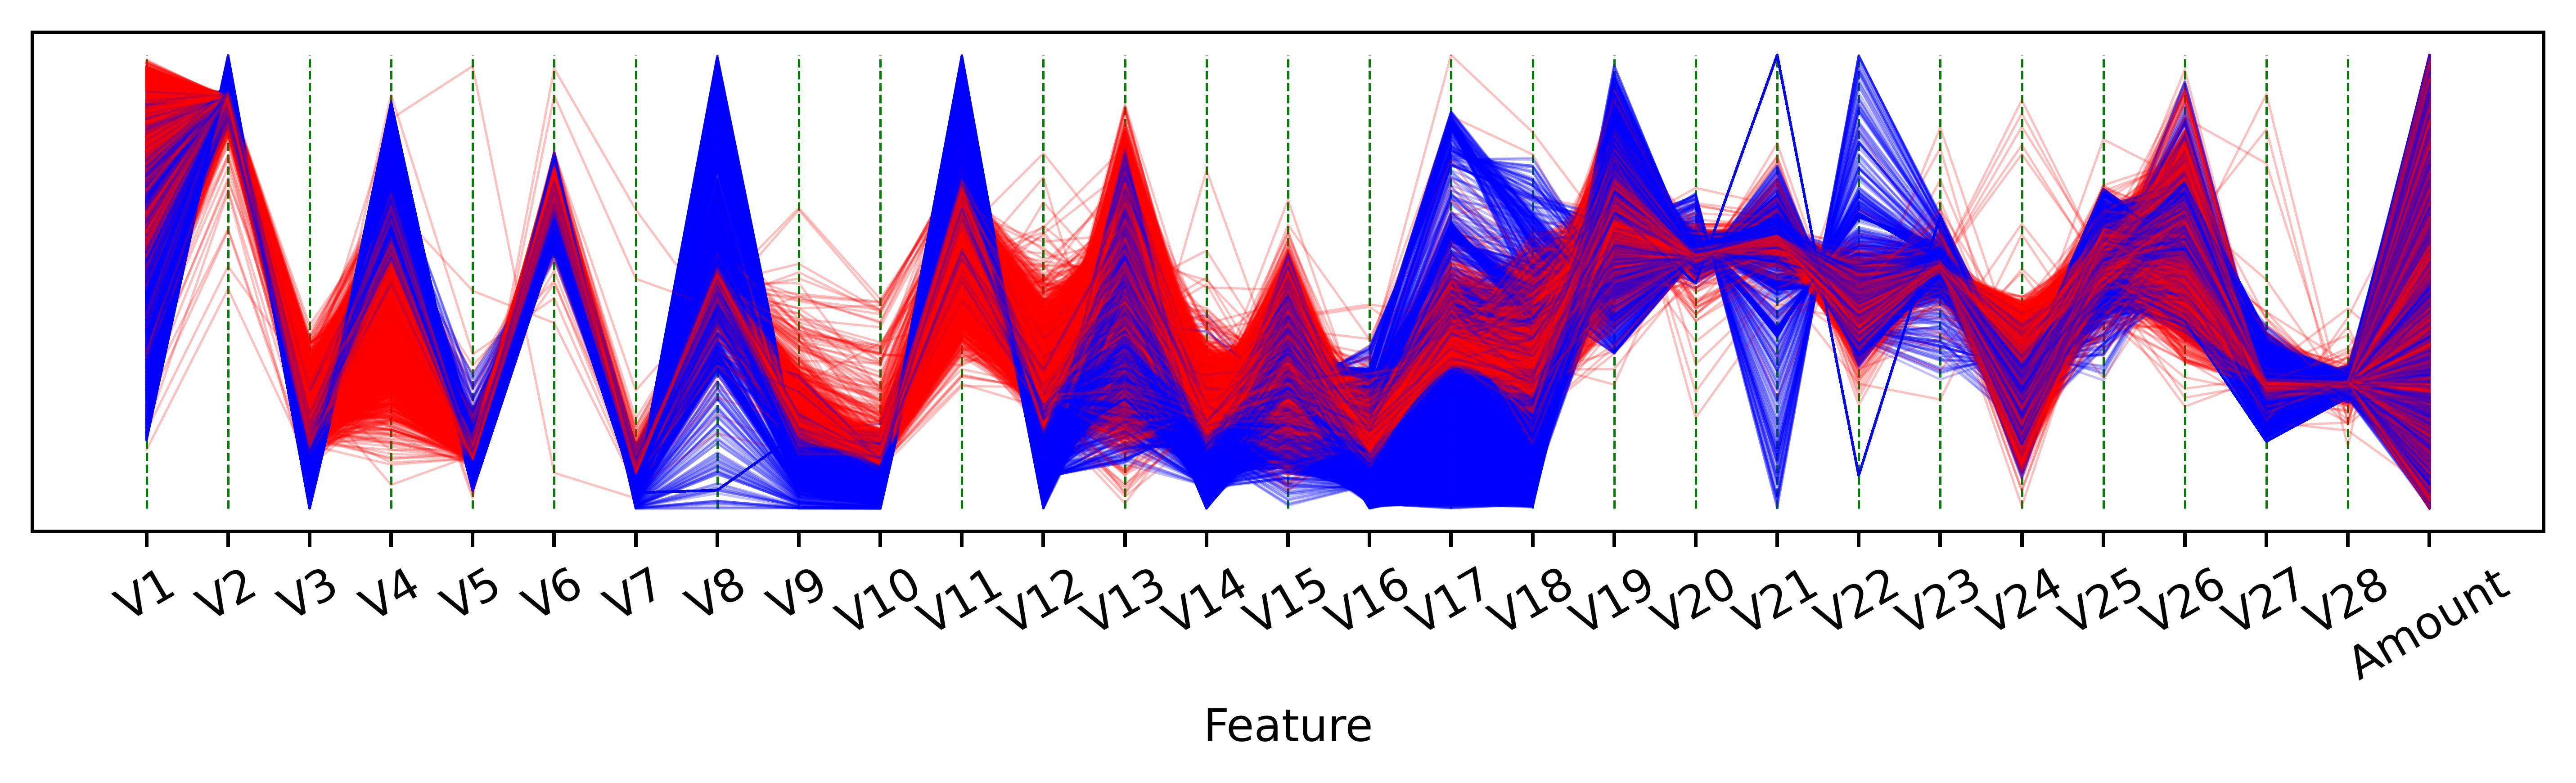
\includegraphics[width=\textwidth]{../code/Task3/Analysis/PC.jpg}
  \caption{The parallel coordinate plot for each features (we chose $10\%$ of total data).}
  \label{task-3-data-distribution}
\end{figure}

\begin{figure}[H]
  \centering
  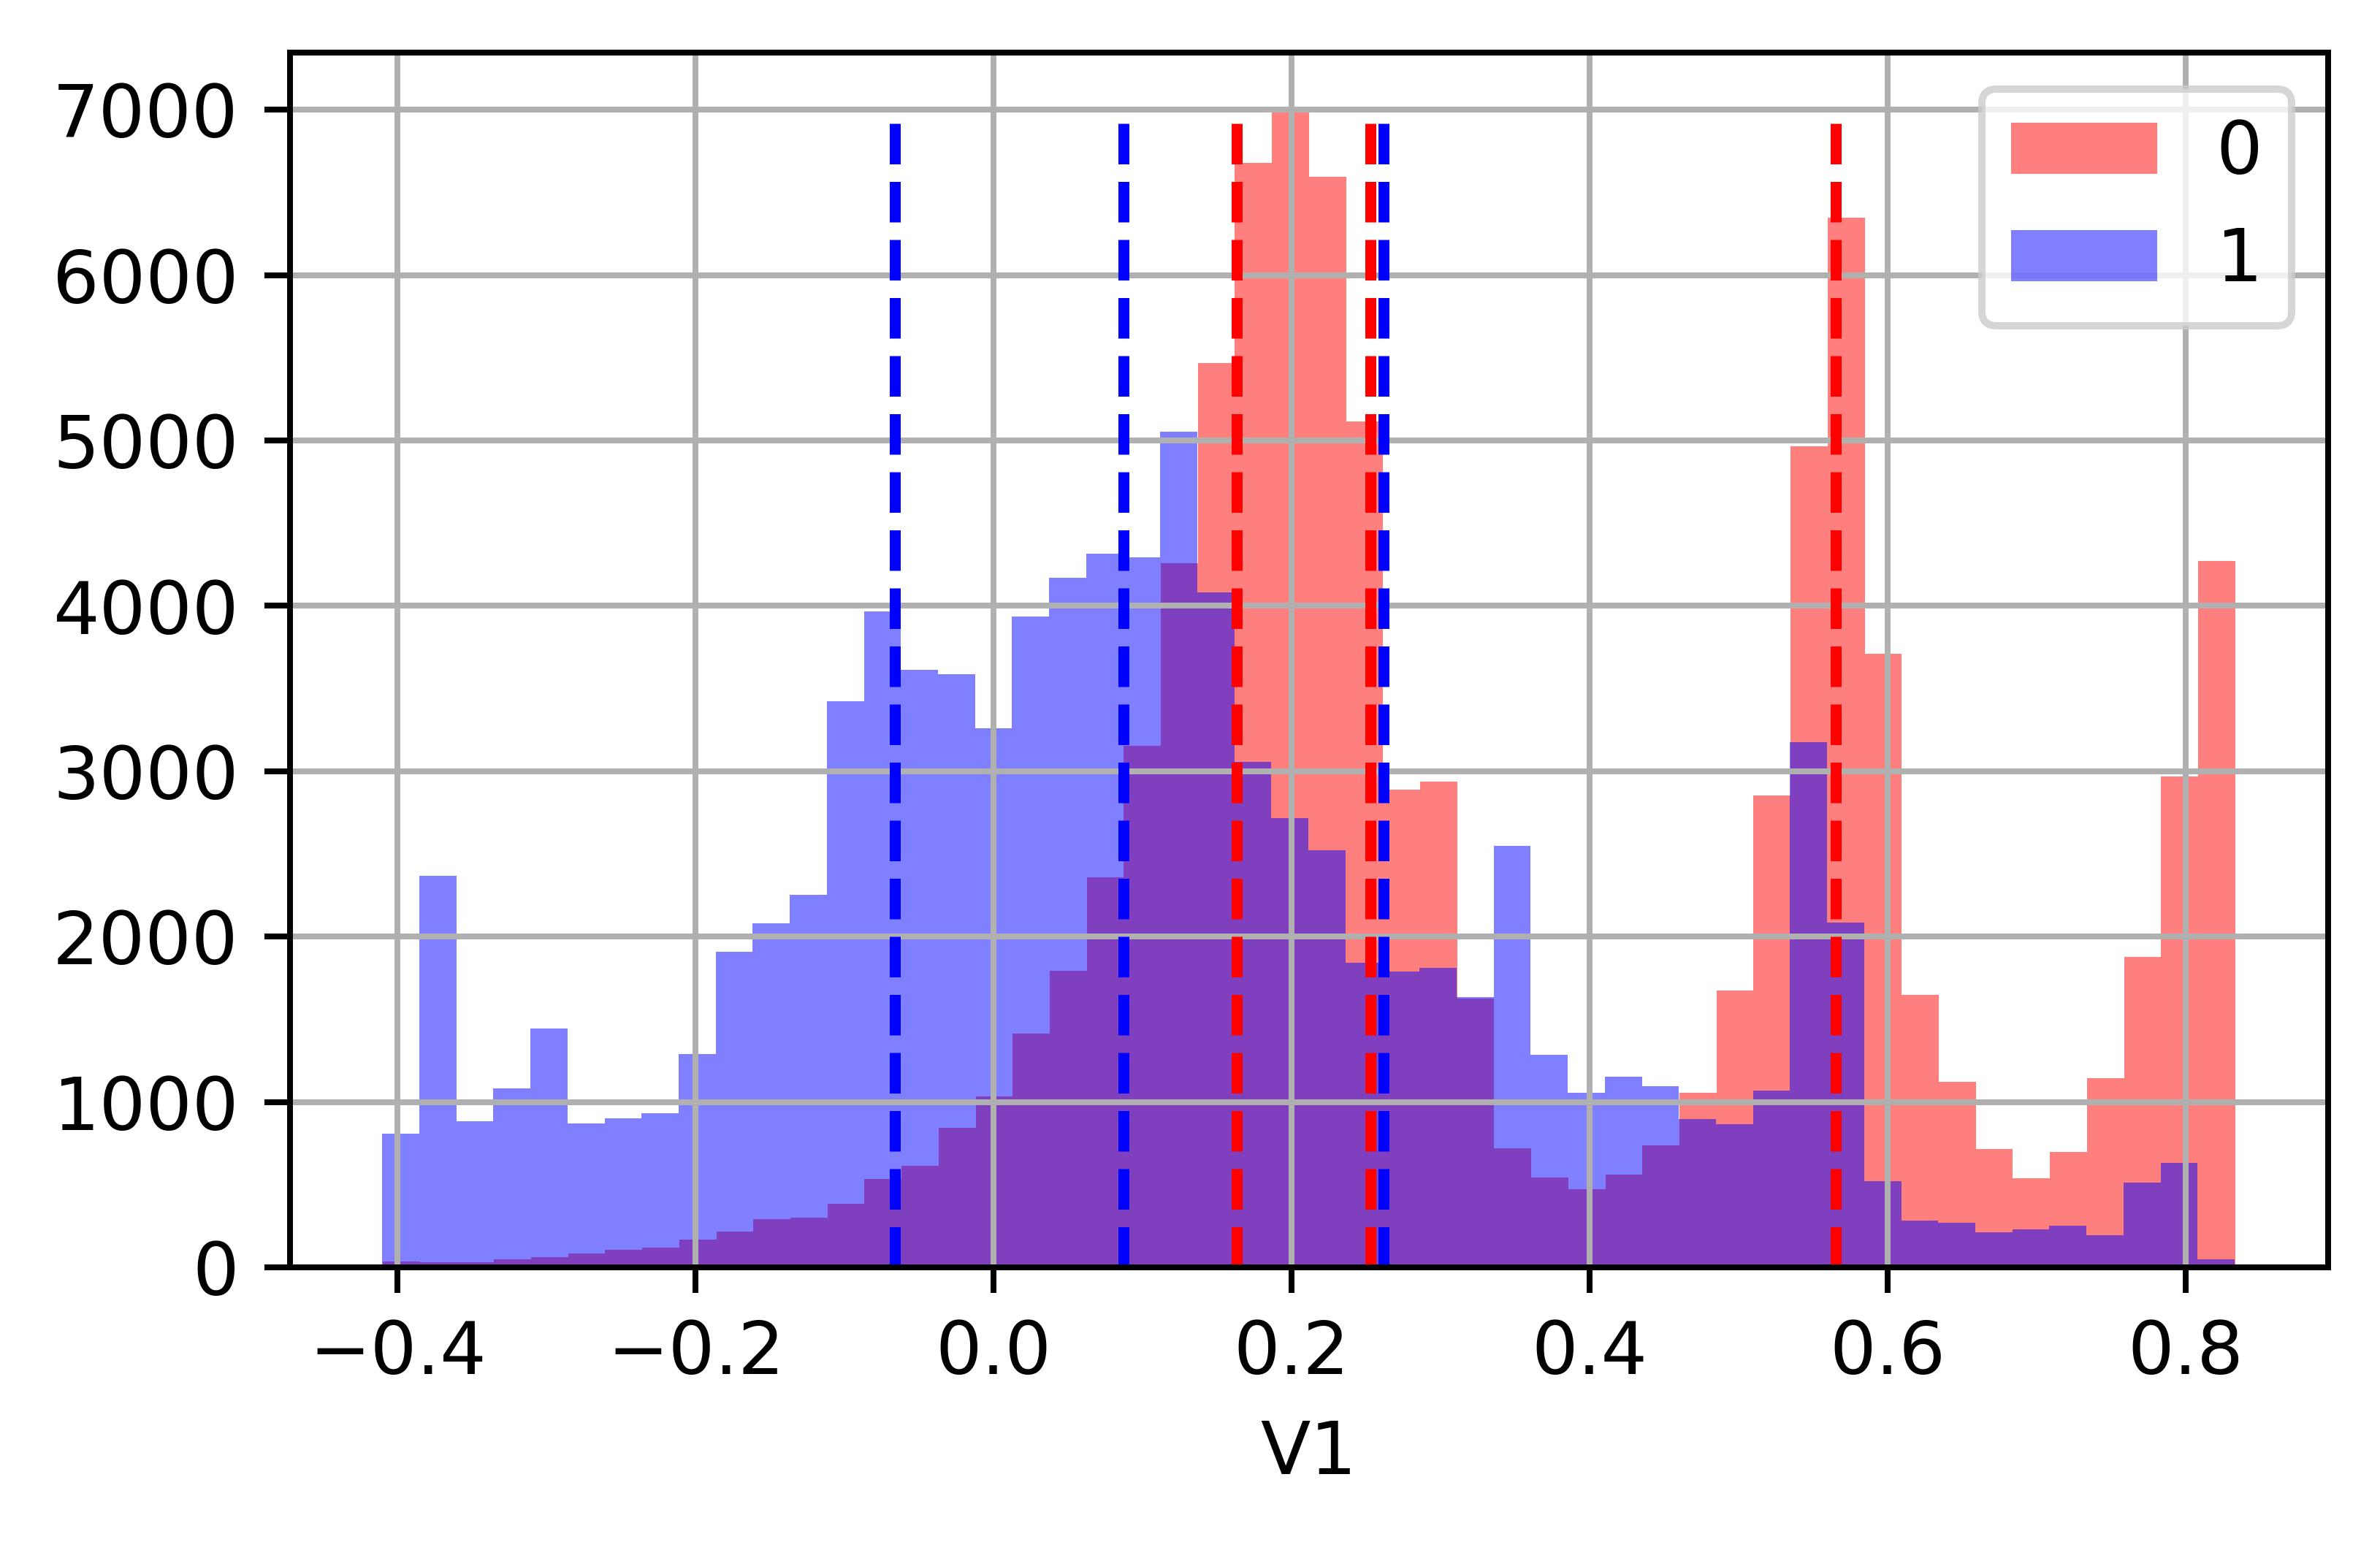
\includegraphics[width=0.18\textwidth]{../code/Task3/Analysis/Hist-V1.jpg}
  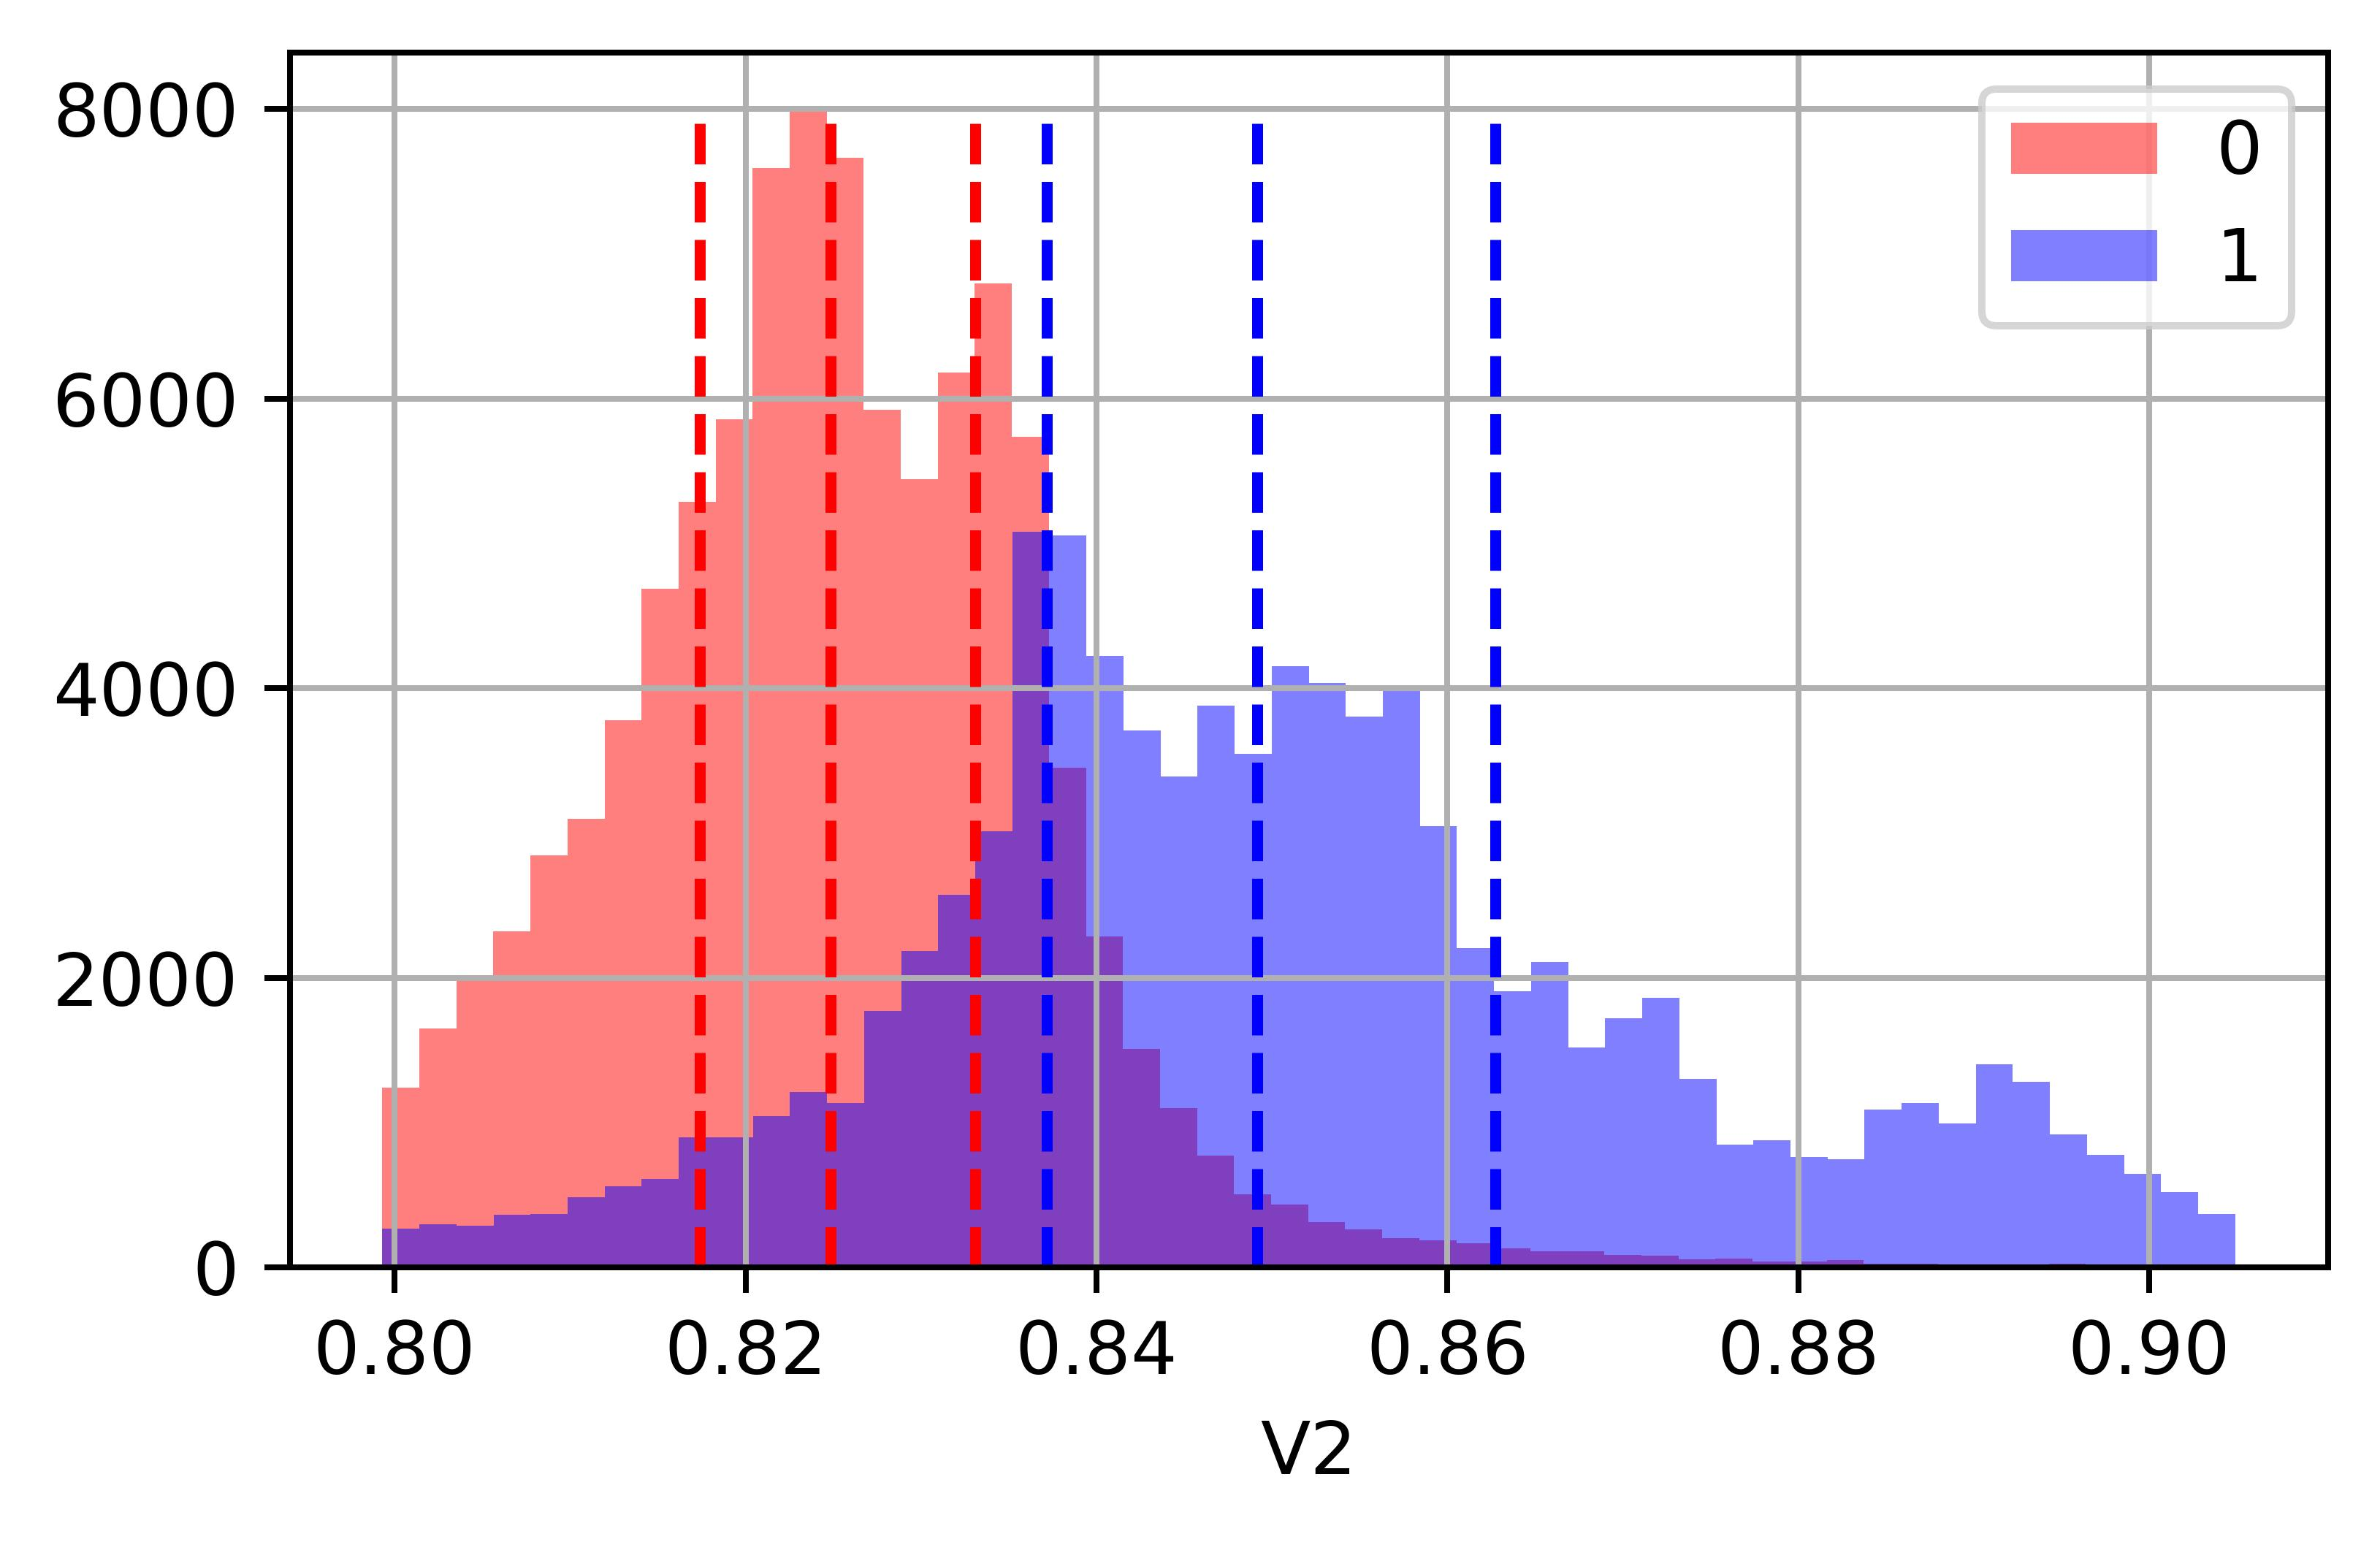
\includegraphics[width=0.18\textwidth]{../code/Task3/Analysis/Hist-V2.jpg}
  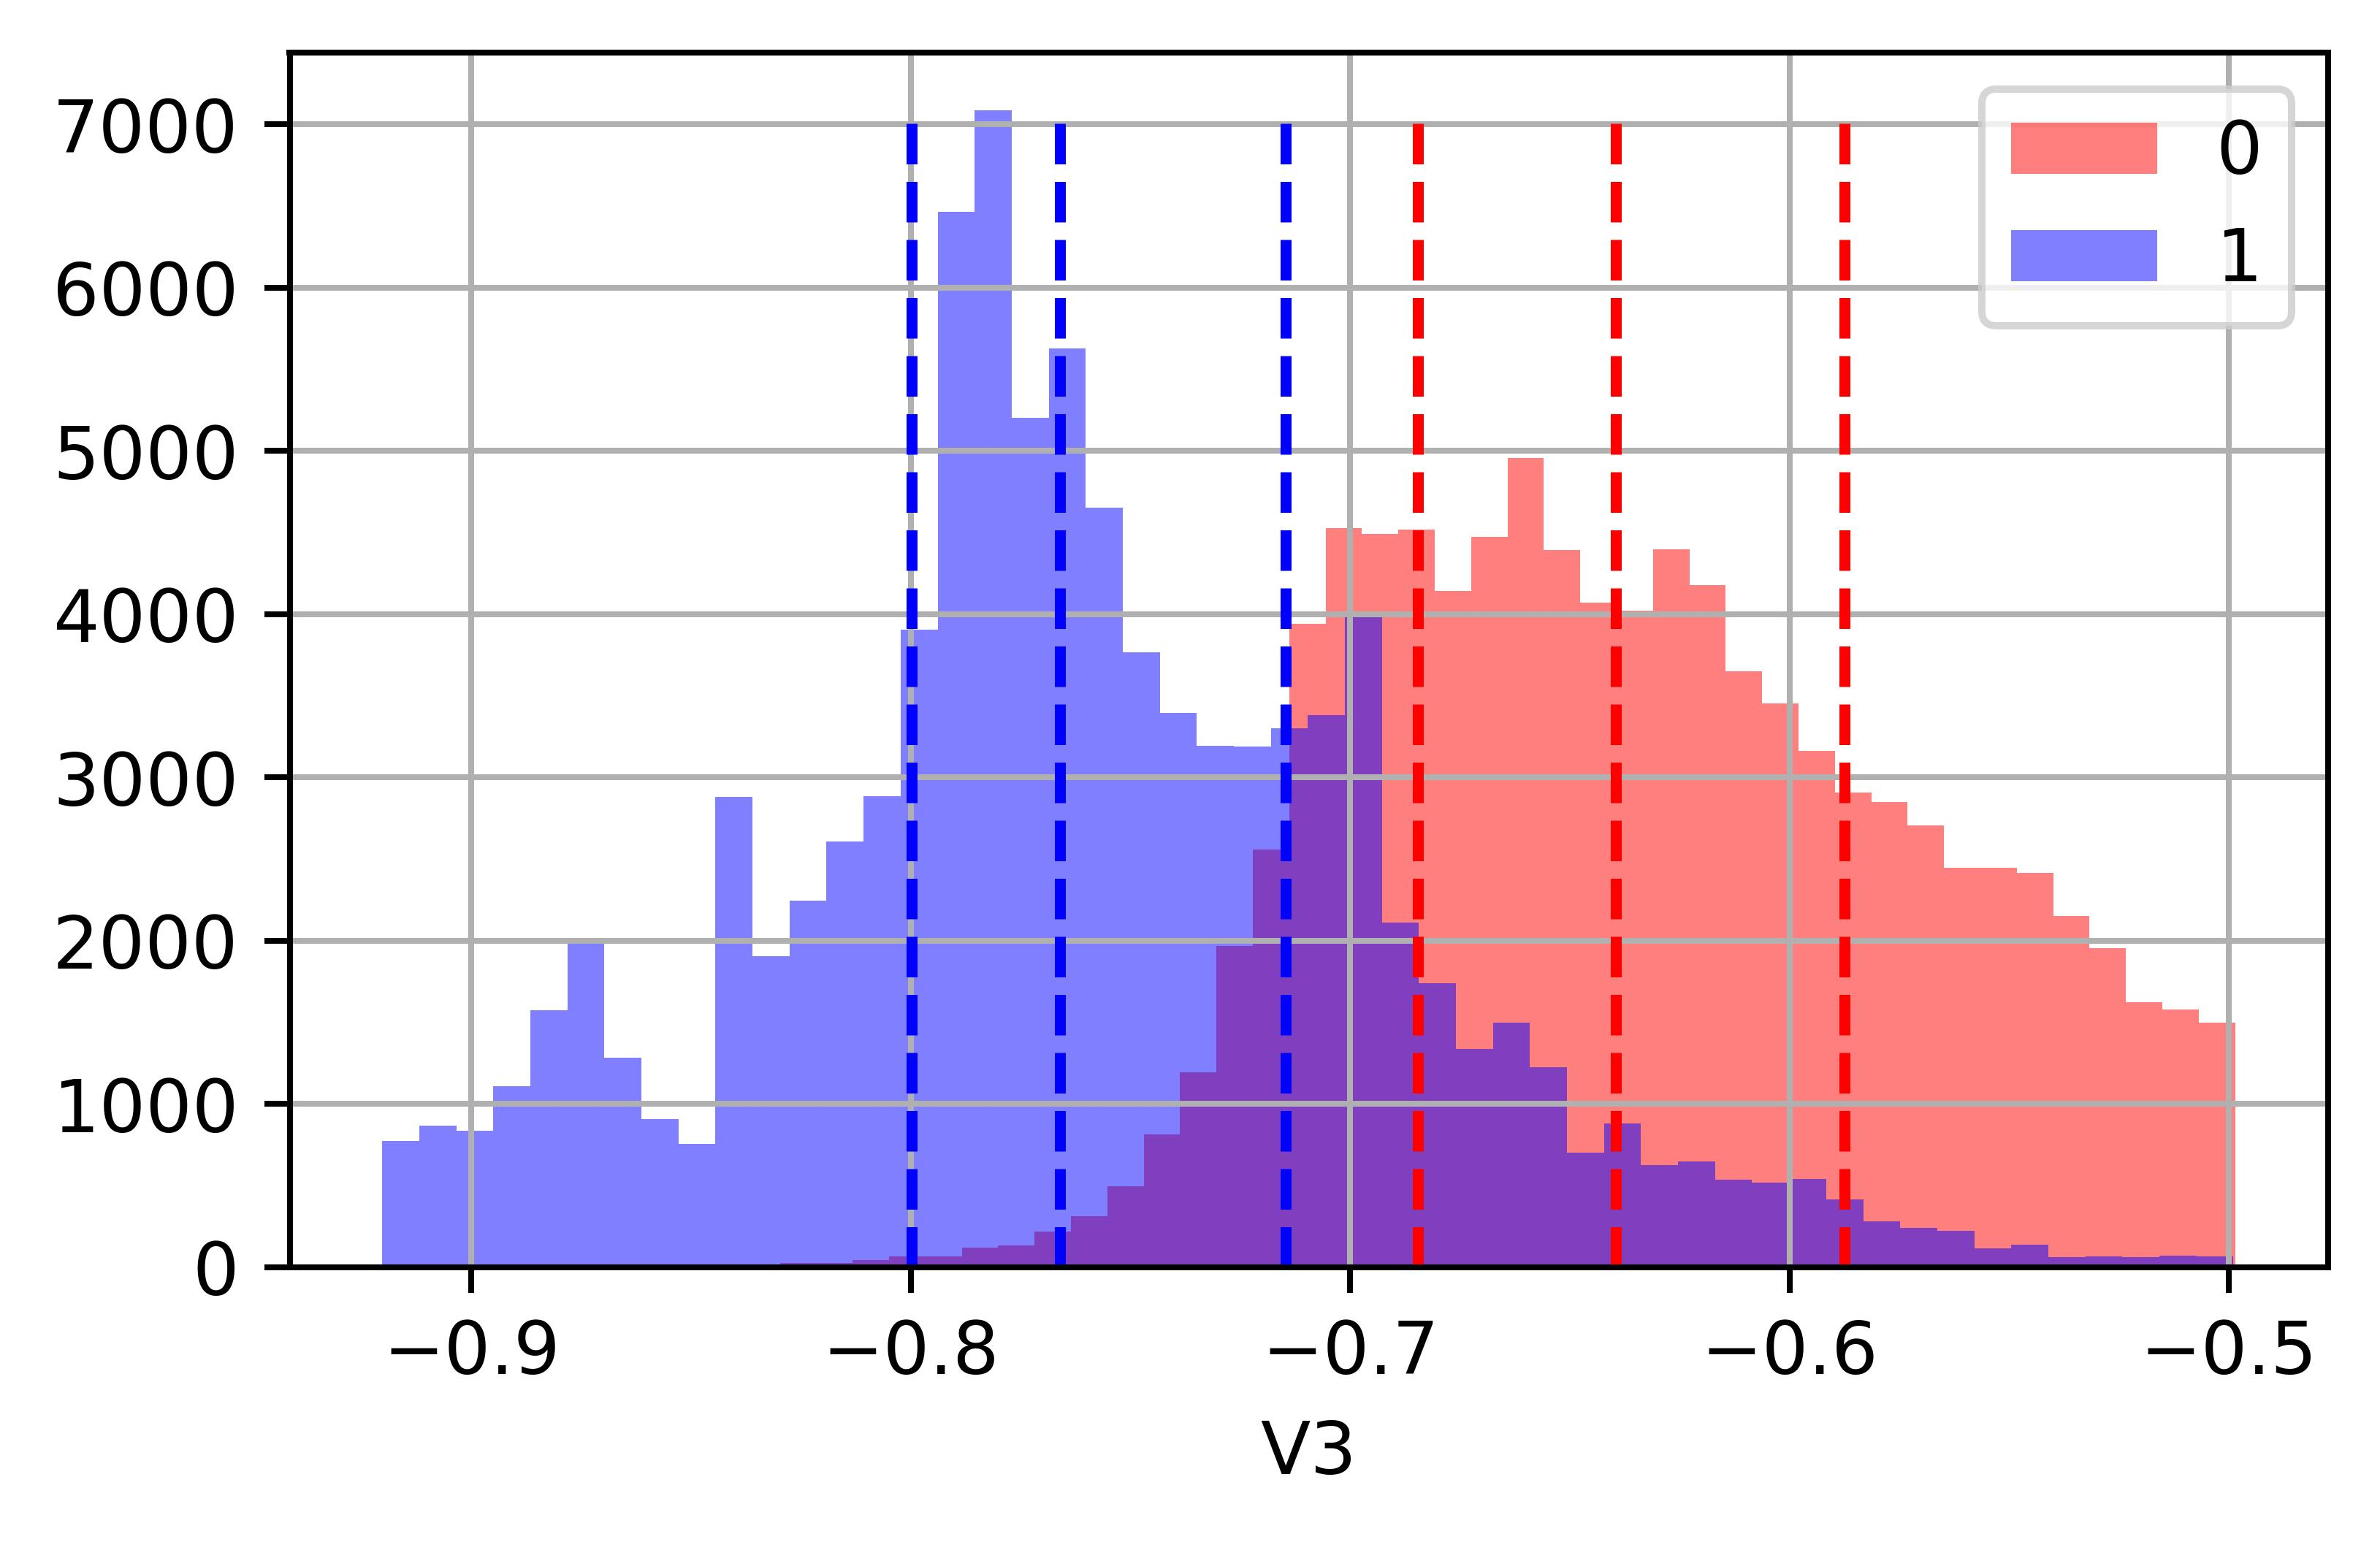
\includegraphics[width=0.18\textwidth]{../code/Task3/Analysis/Hist-V3.jpg}
  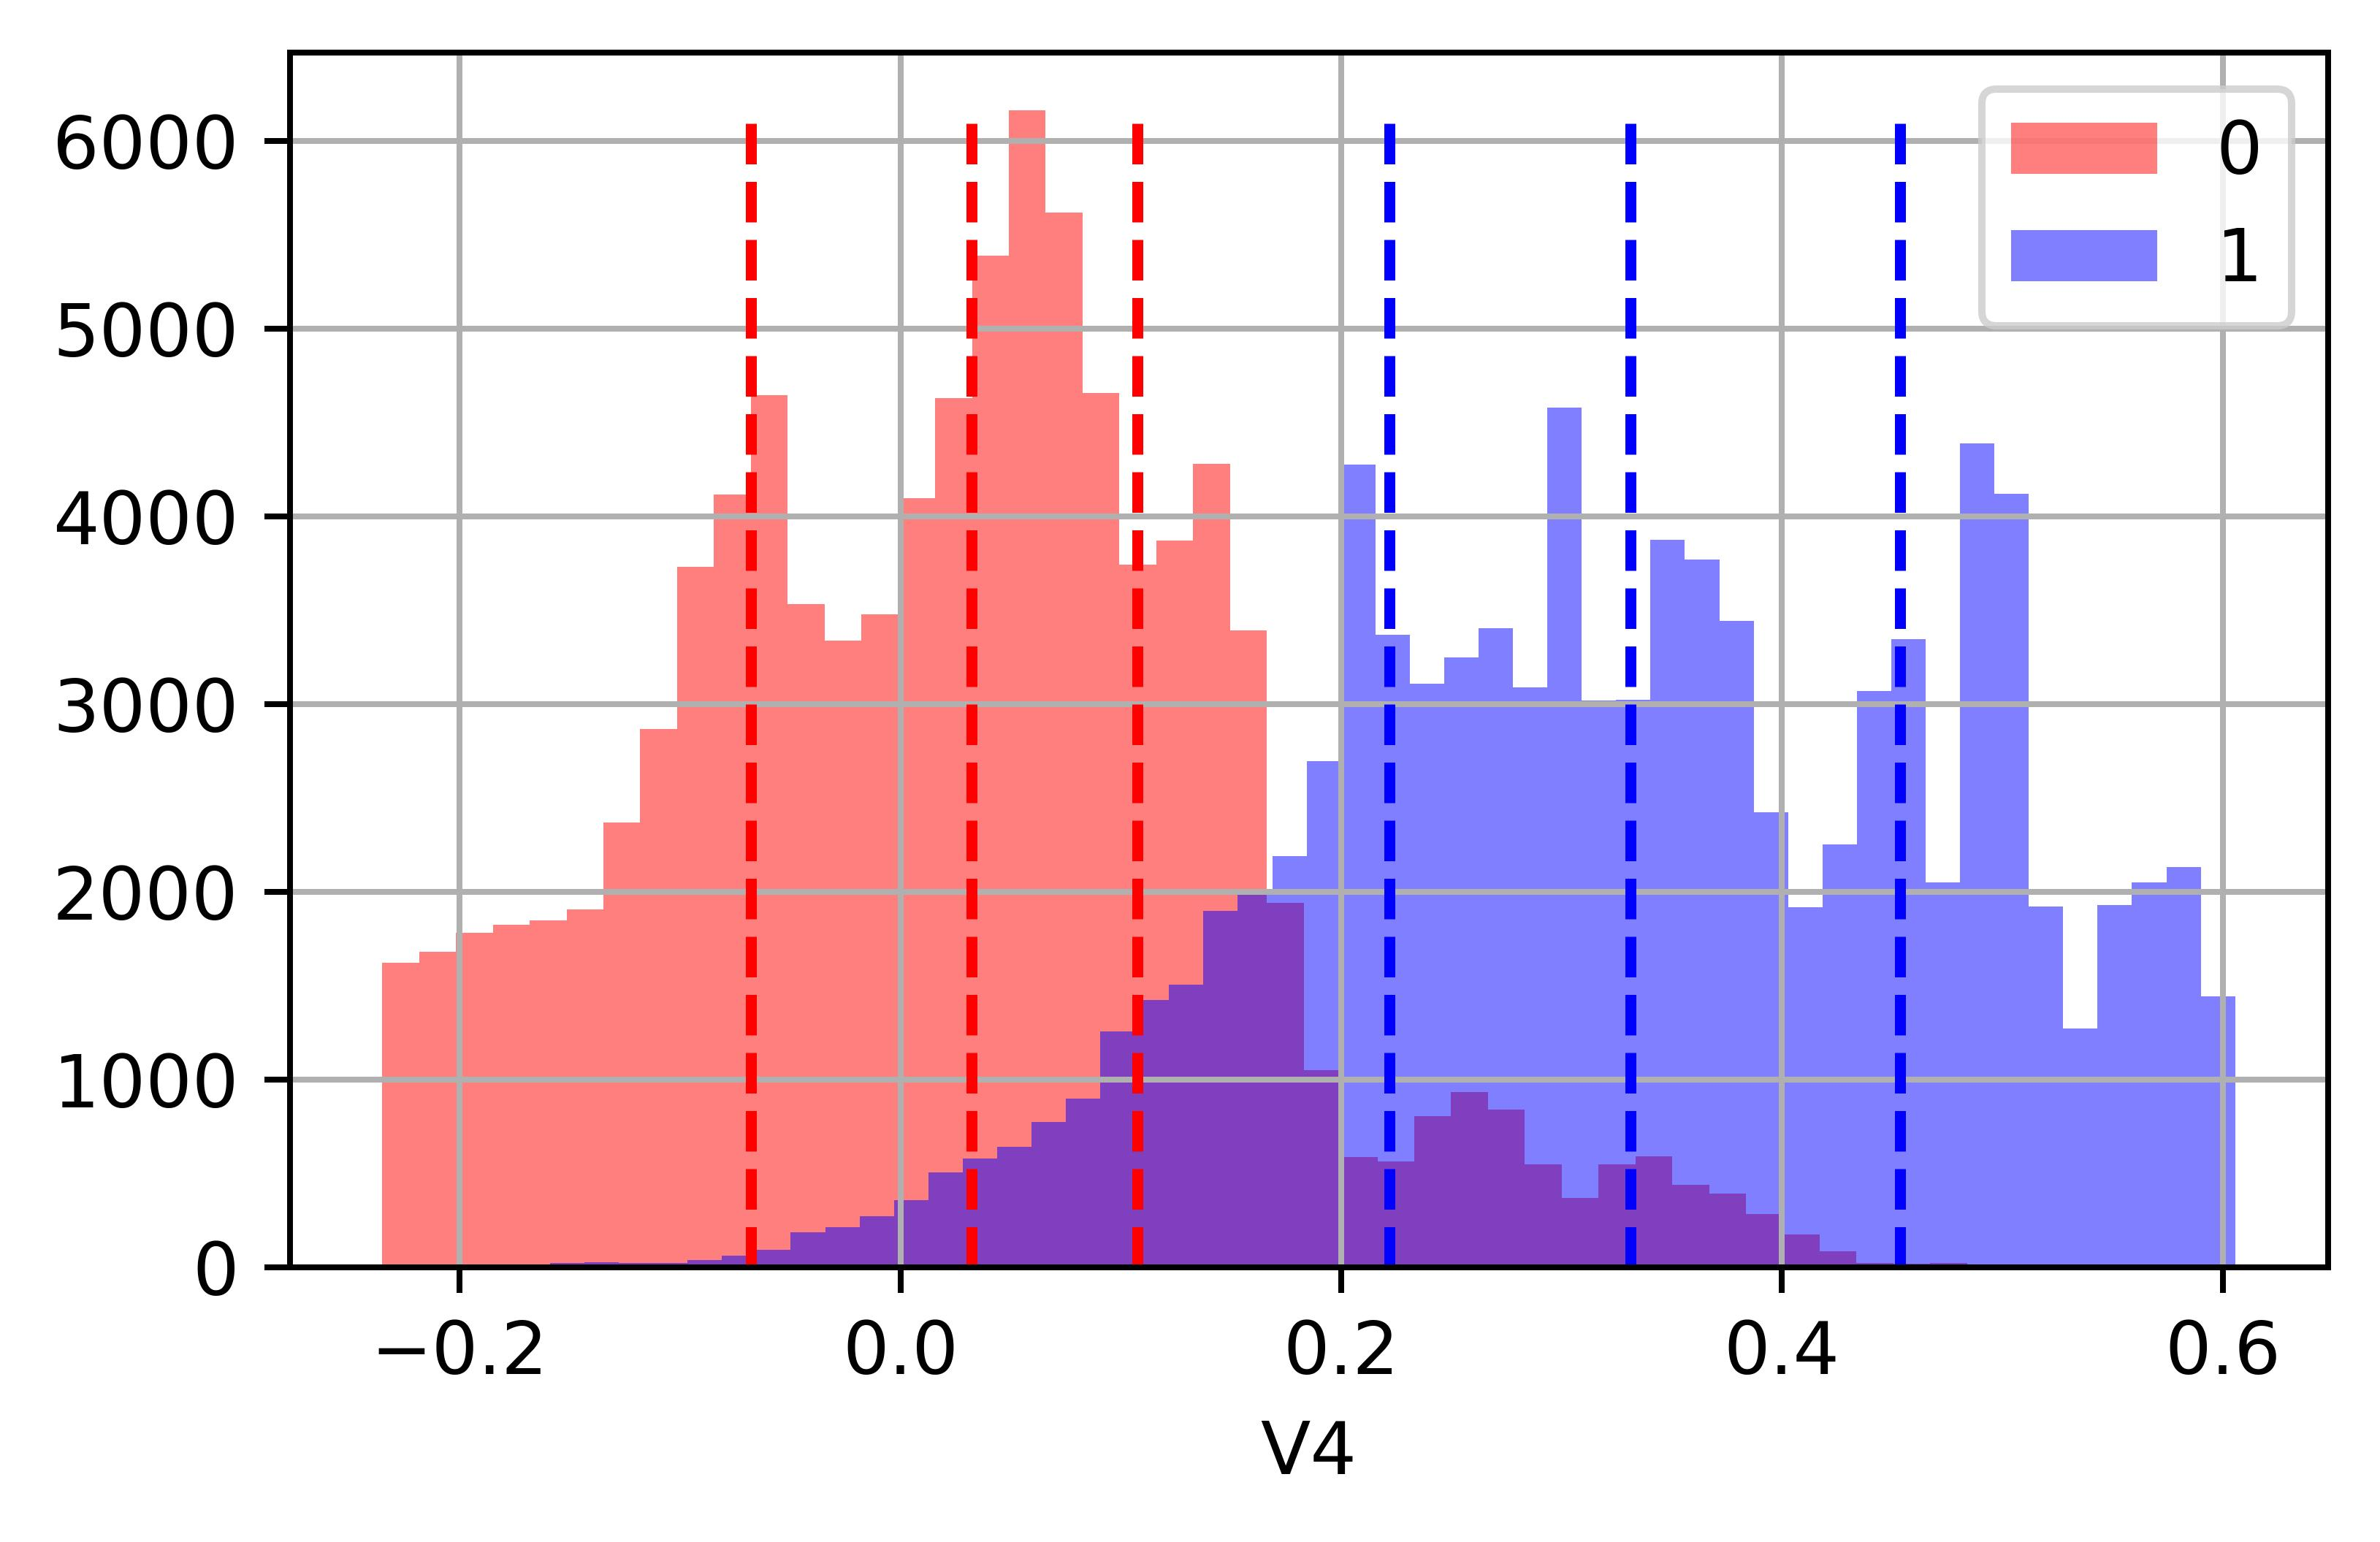
\includegraphics[width=0.18\textwidth]{../code/Task3/Analysis/Hist-V4.jpg}
  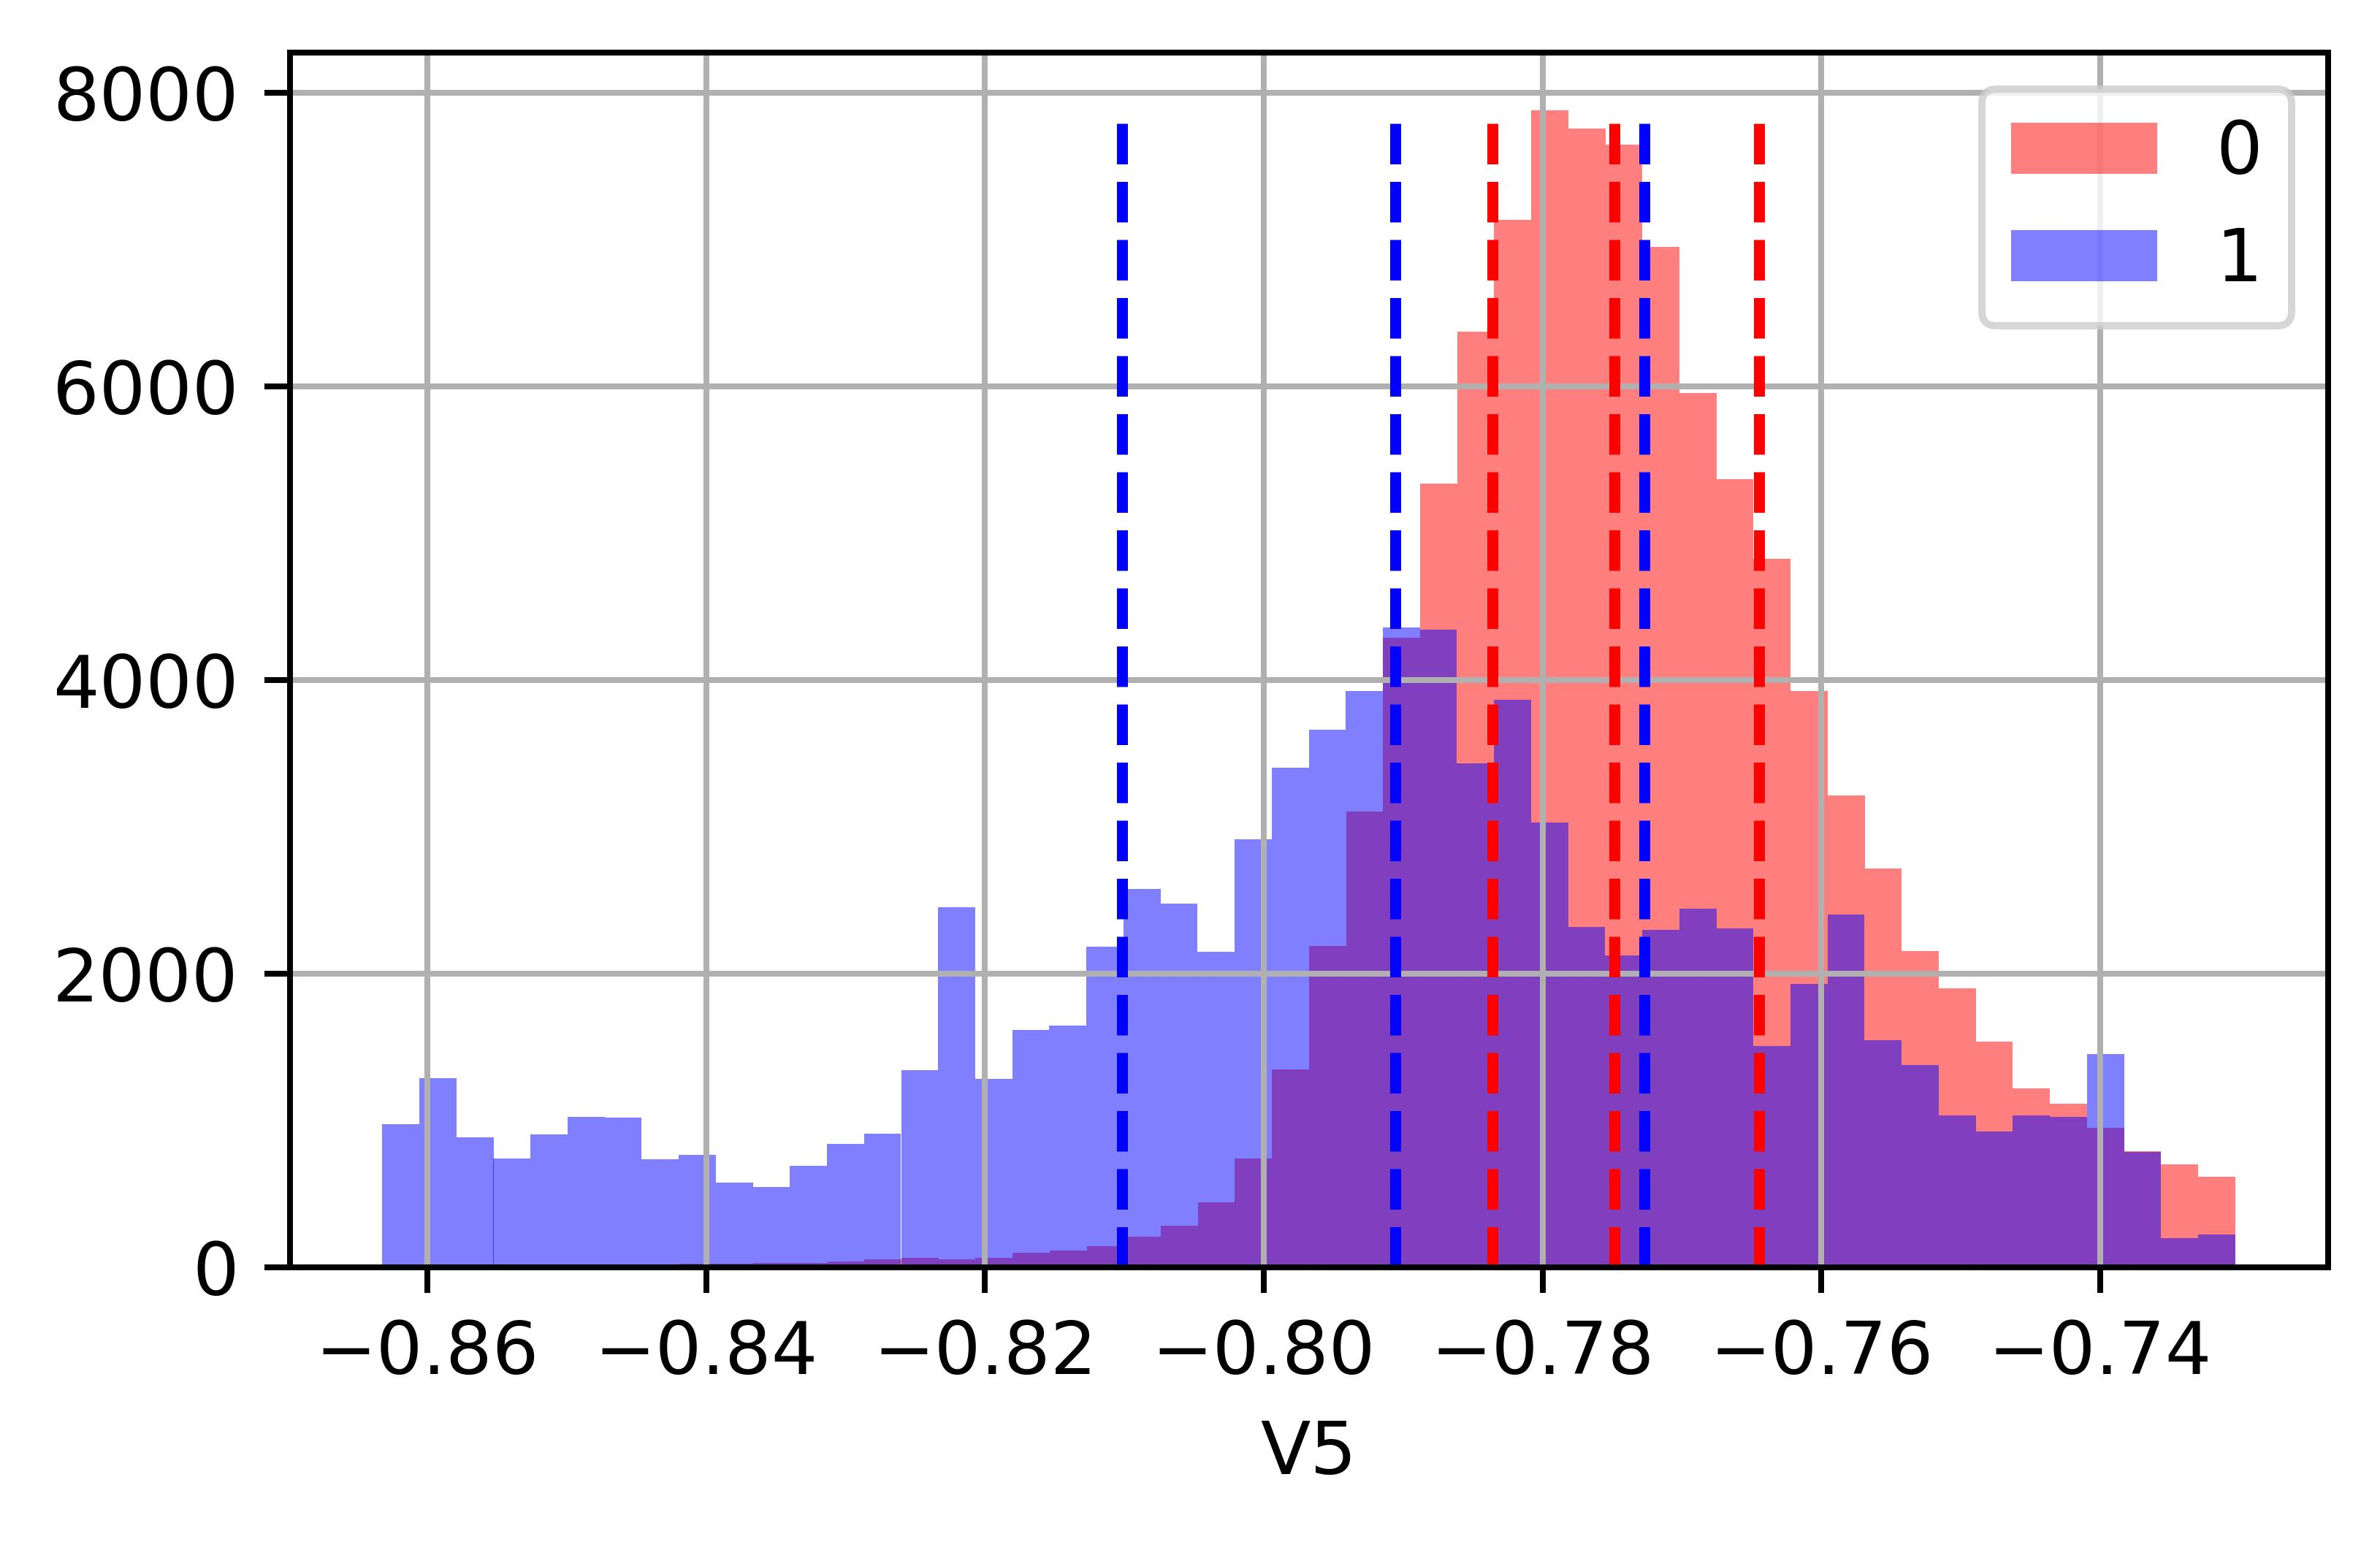
\includegraphics[width=0.18\textwidth]{../code/Task3/Analysis/Hist-V5.jpg} \\
  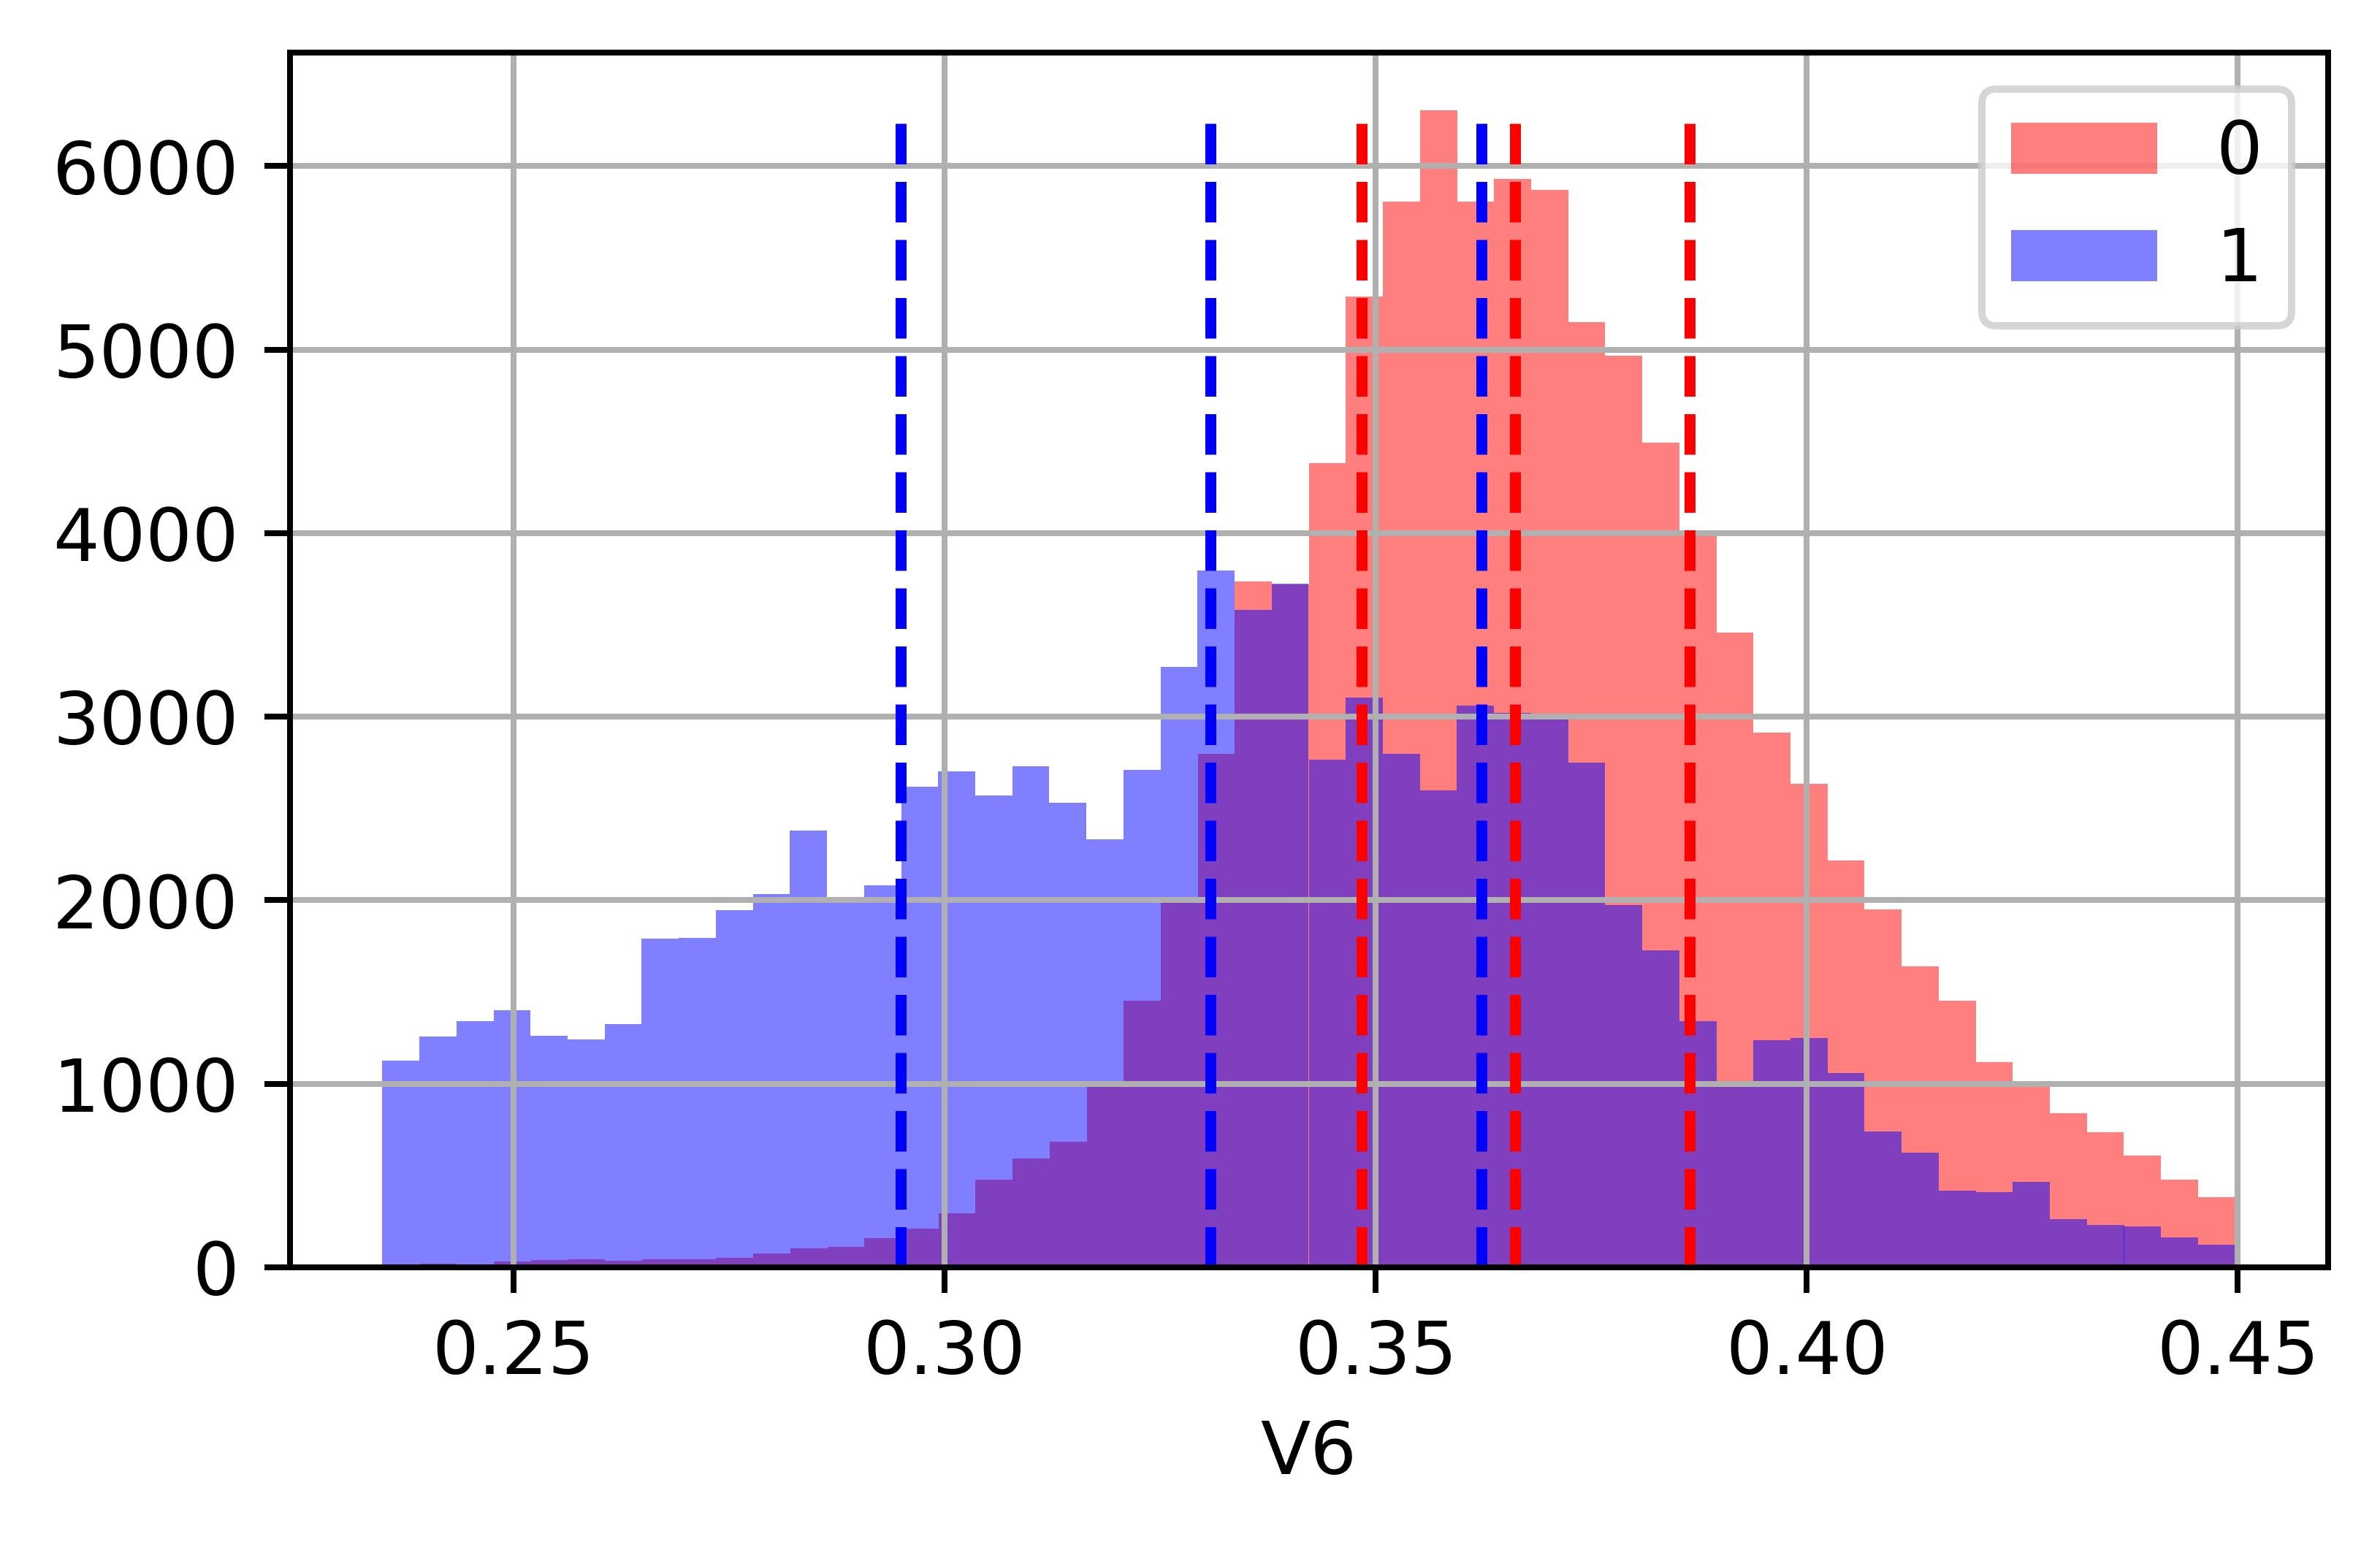
\includegraphics[width=0.18\textwidth]{../code/Task3/Analysis/Hist-V6.jpg}
  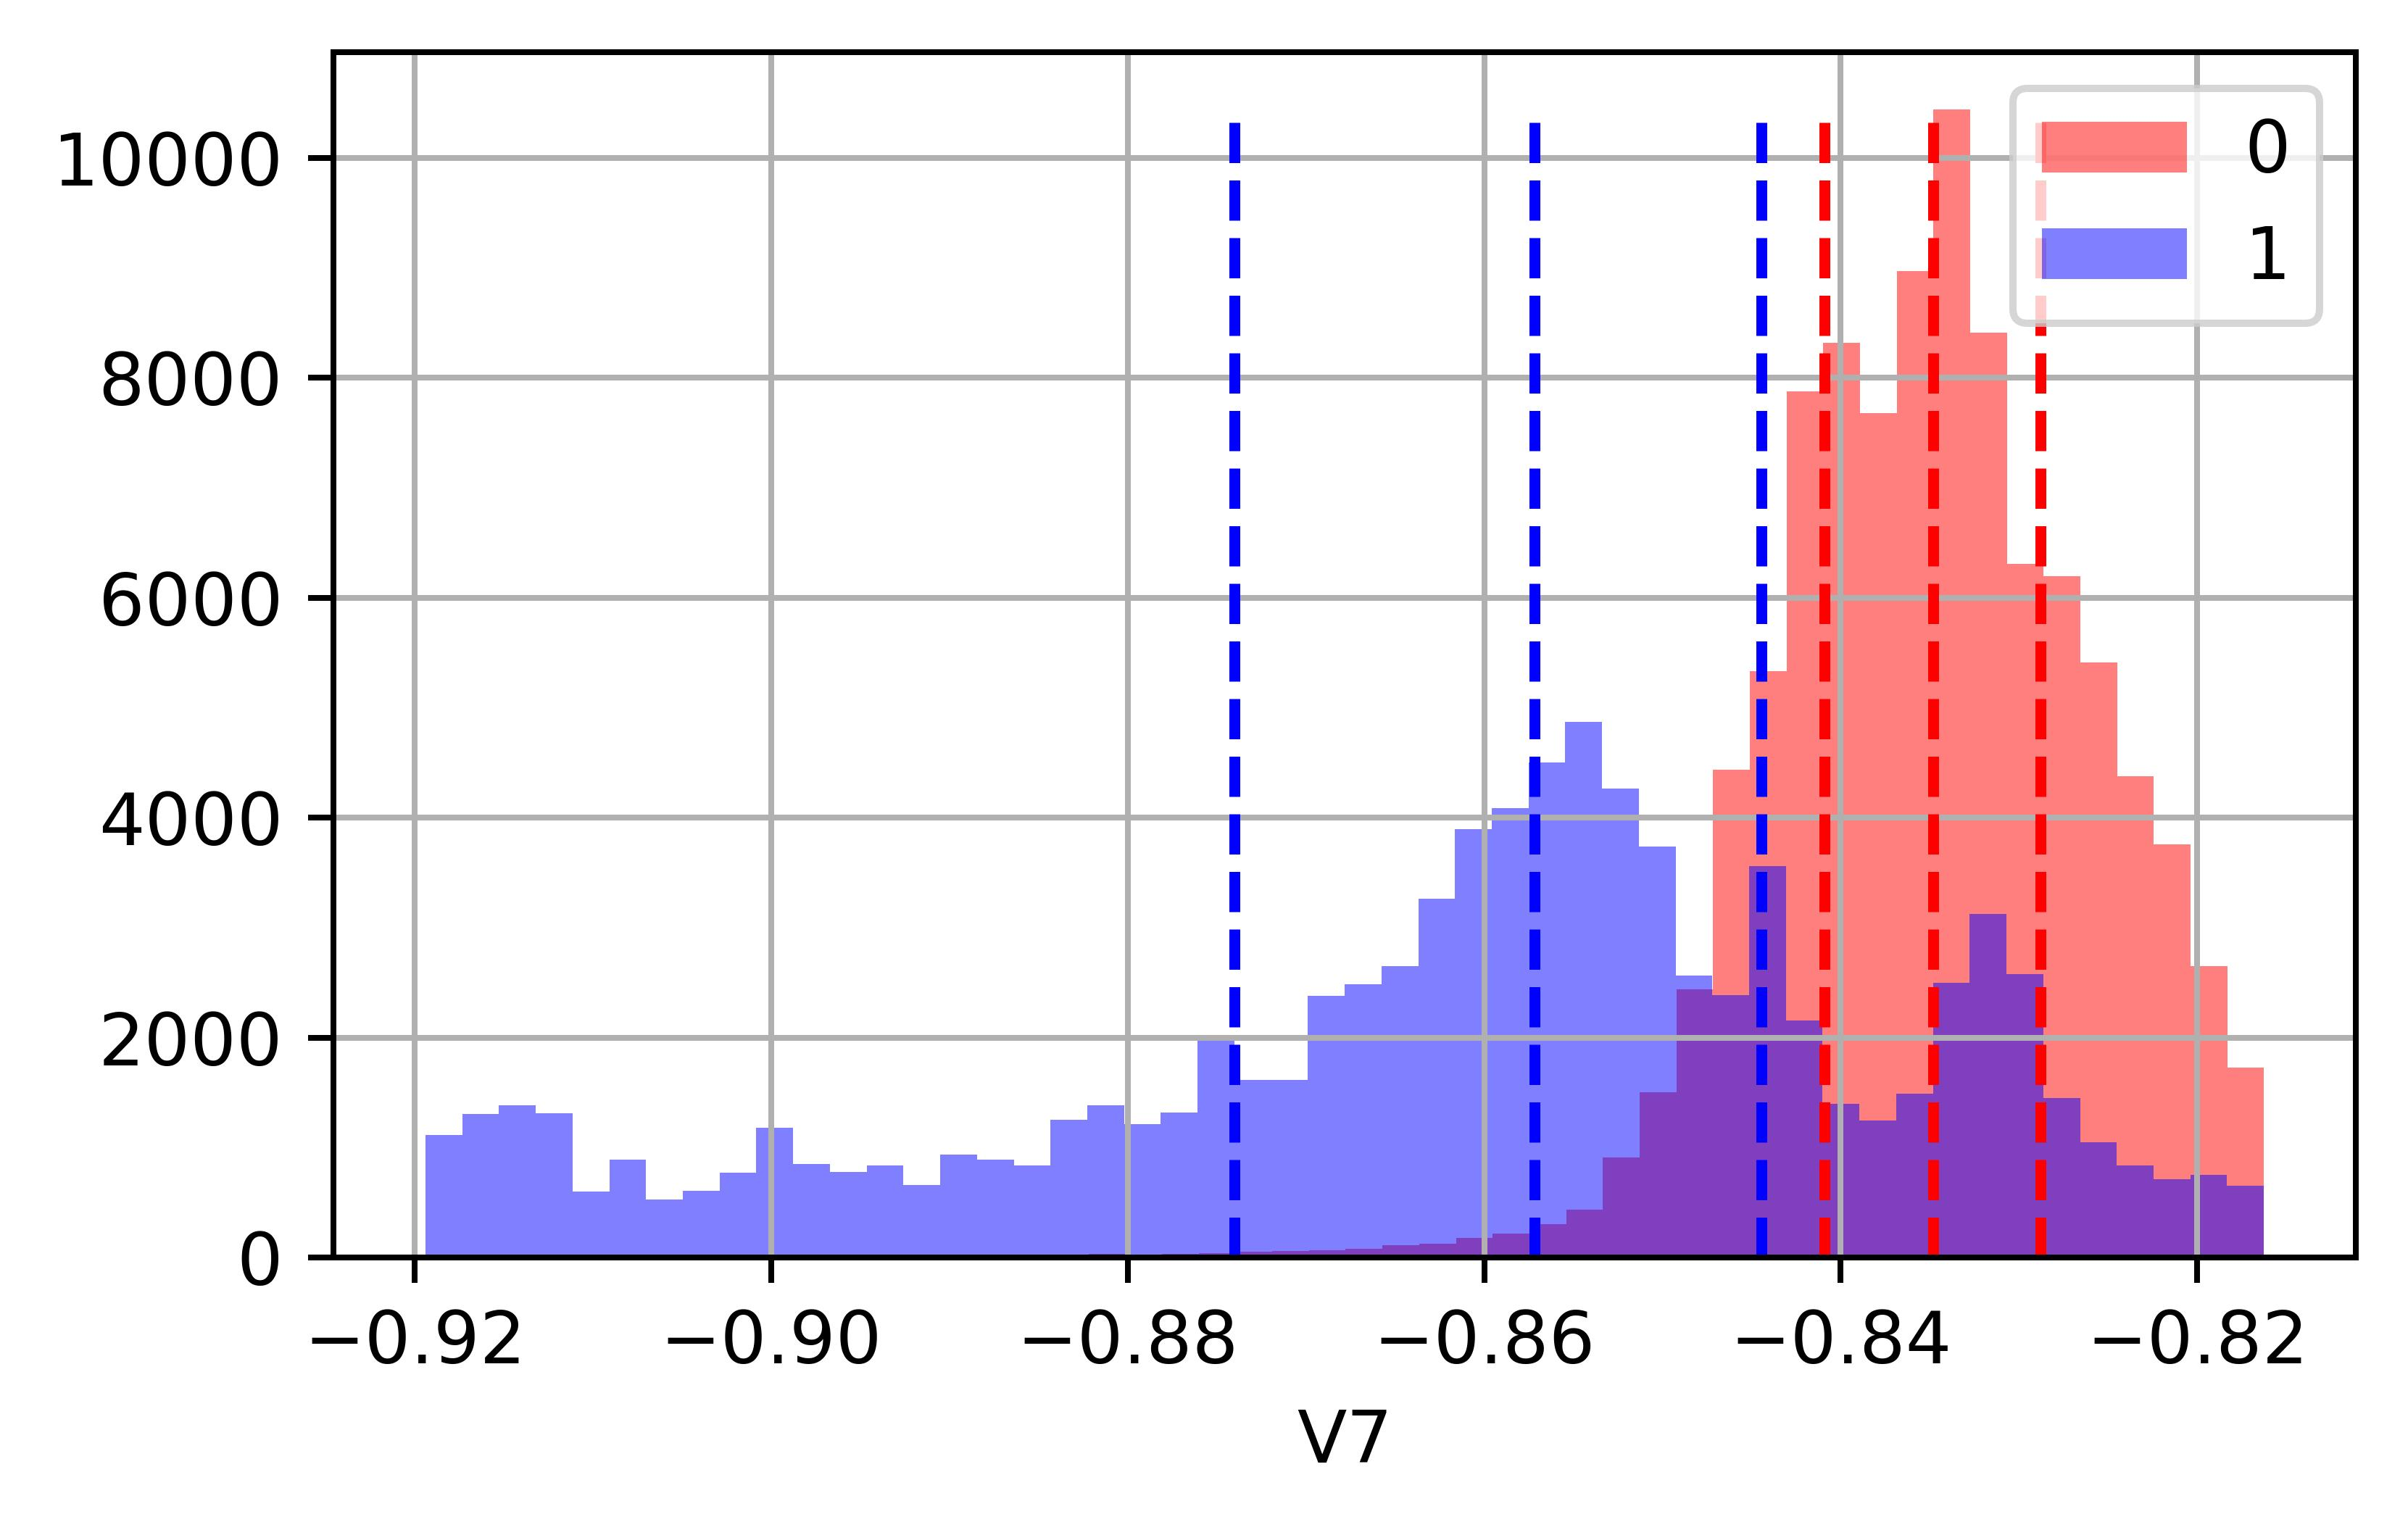
\includegraphics[width=0.18\textwidth]{../code/Task3/Analysis/Hist-V7.jpg}
  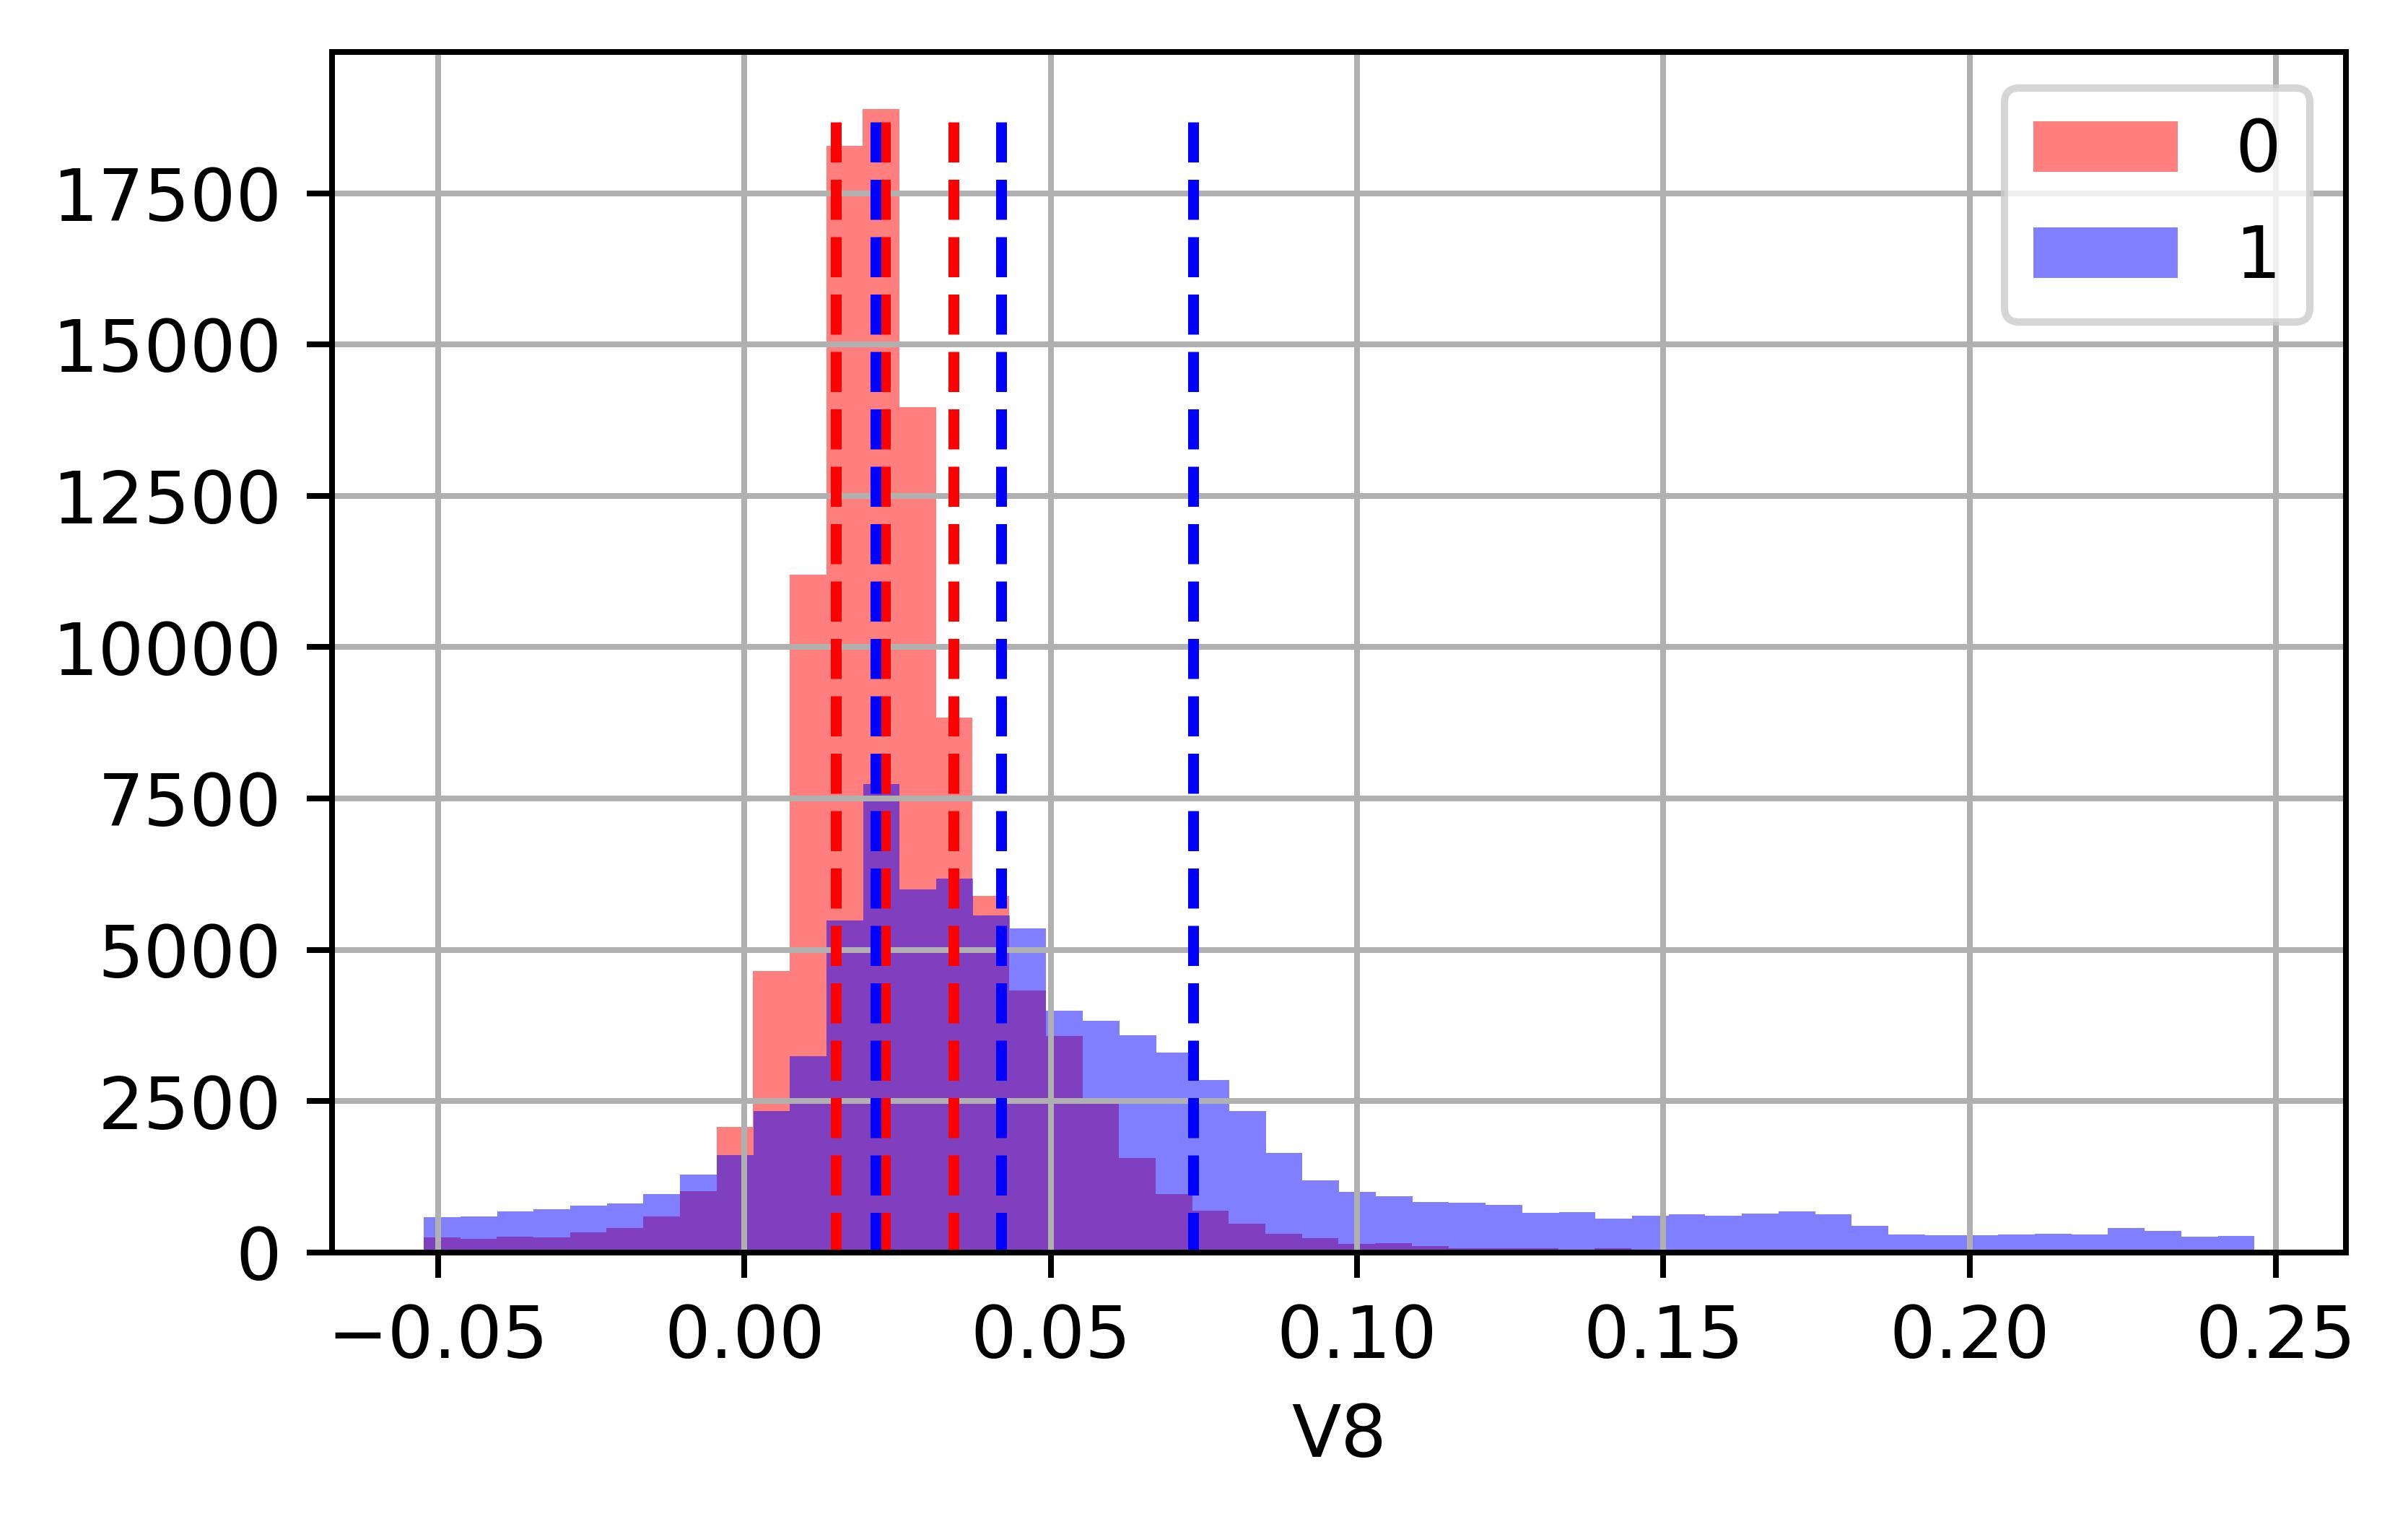
\includegraphics[width=0.18\textwidth]{../code/Task3/Analysis/Hist-V8.jpg}
  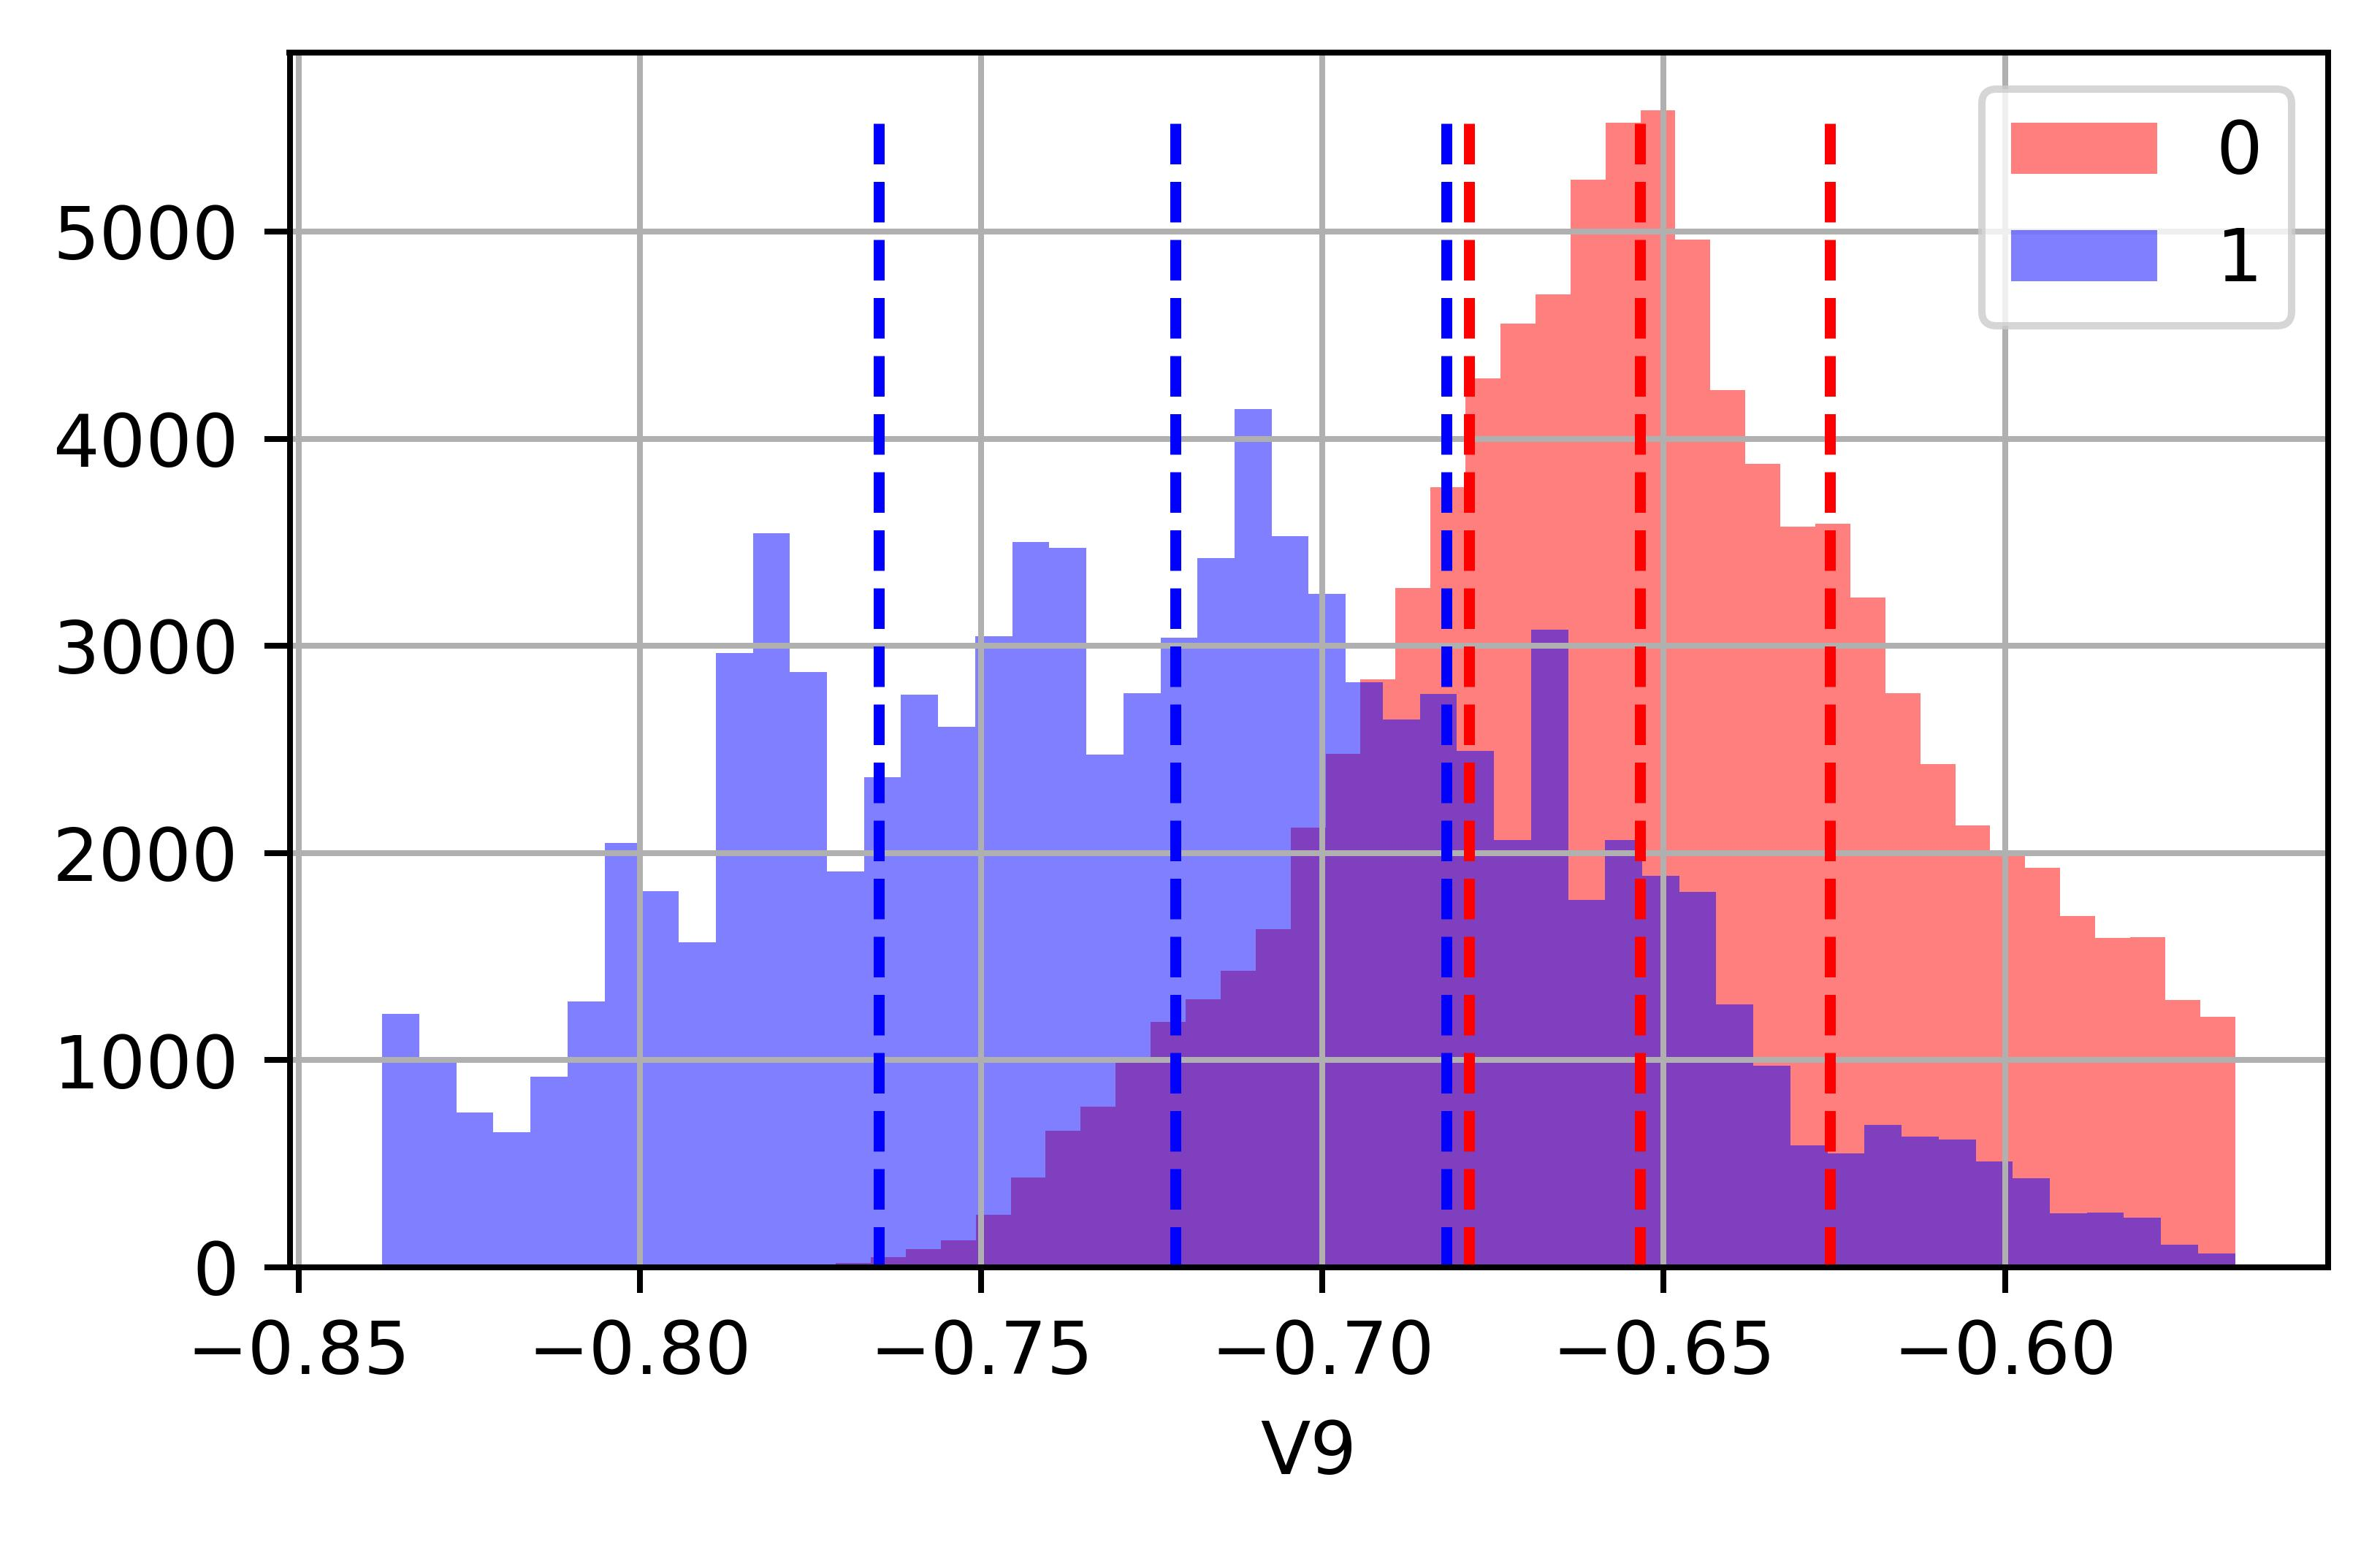
\includegraphics[width=0.18\textwidth]{../code/Task3/Analysis/Hist-V9.jpg}
  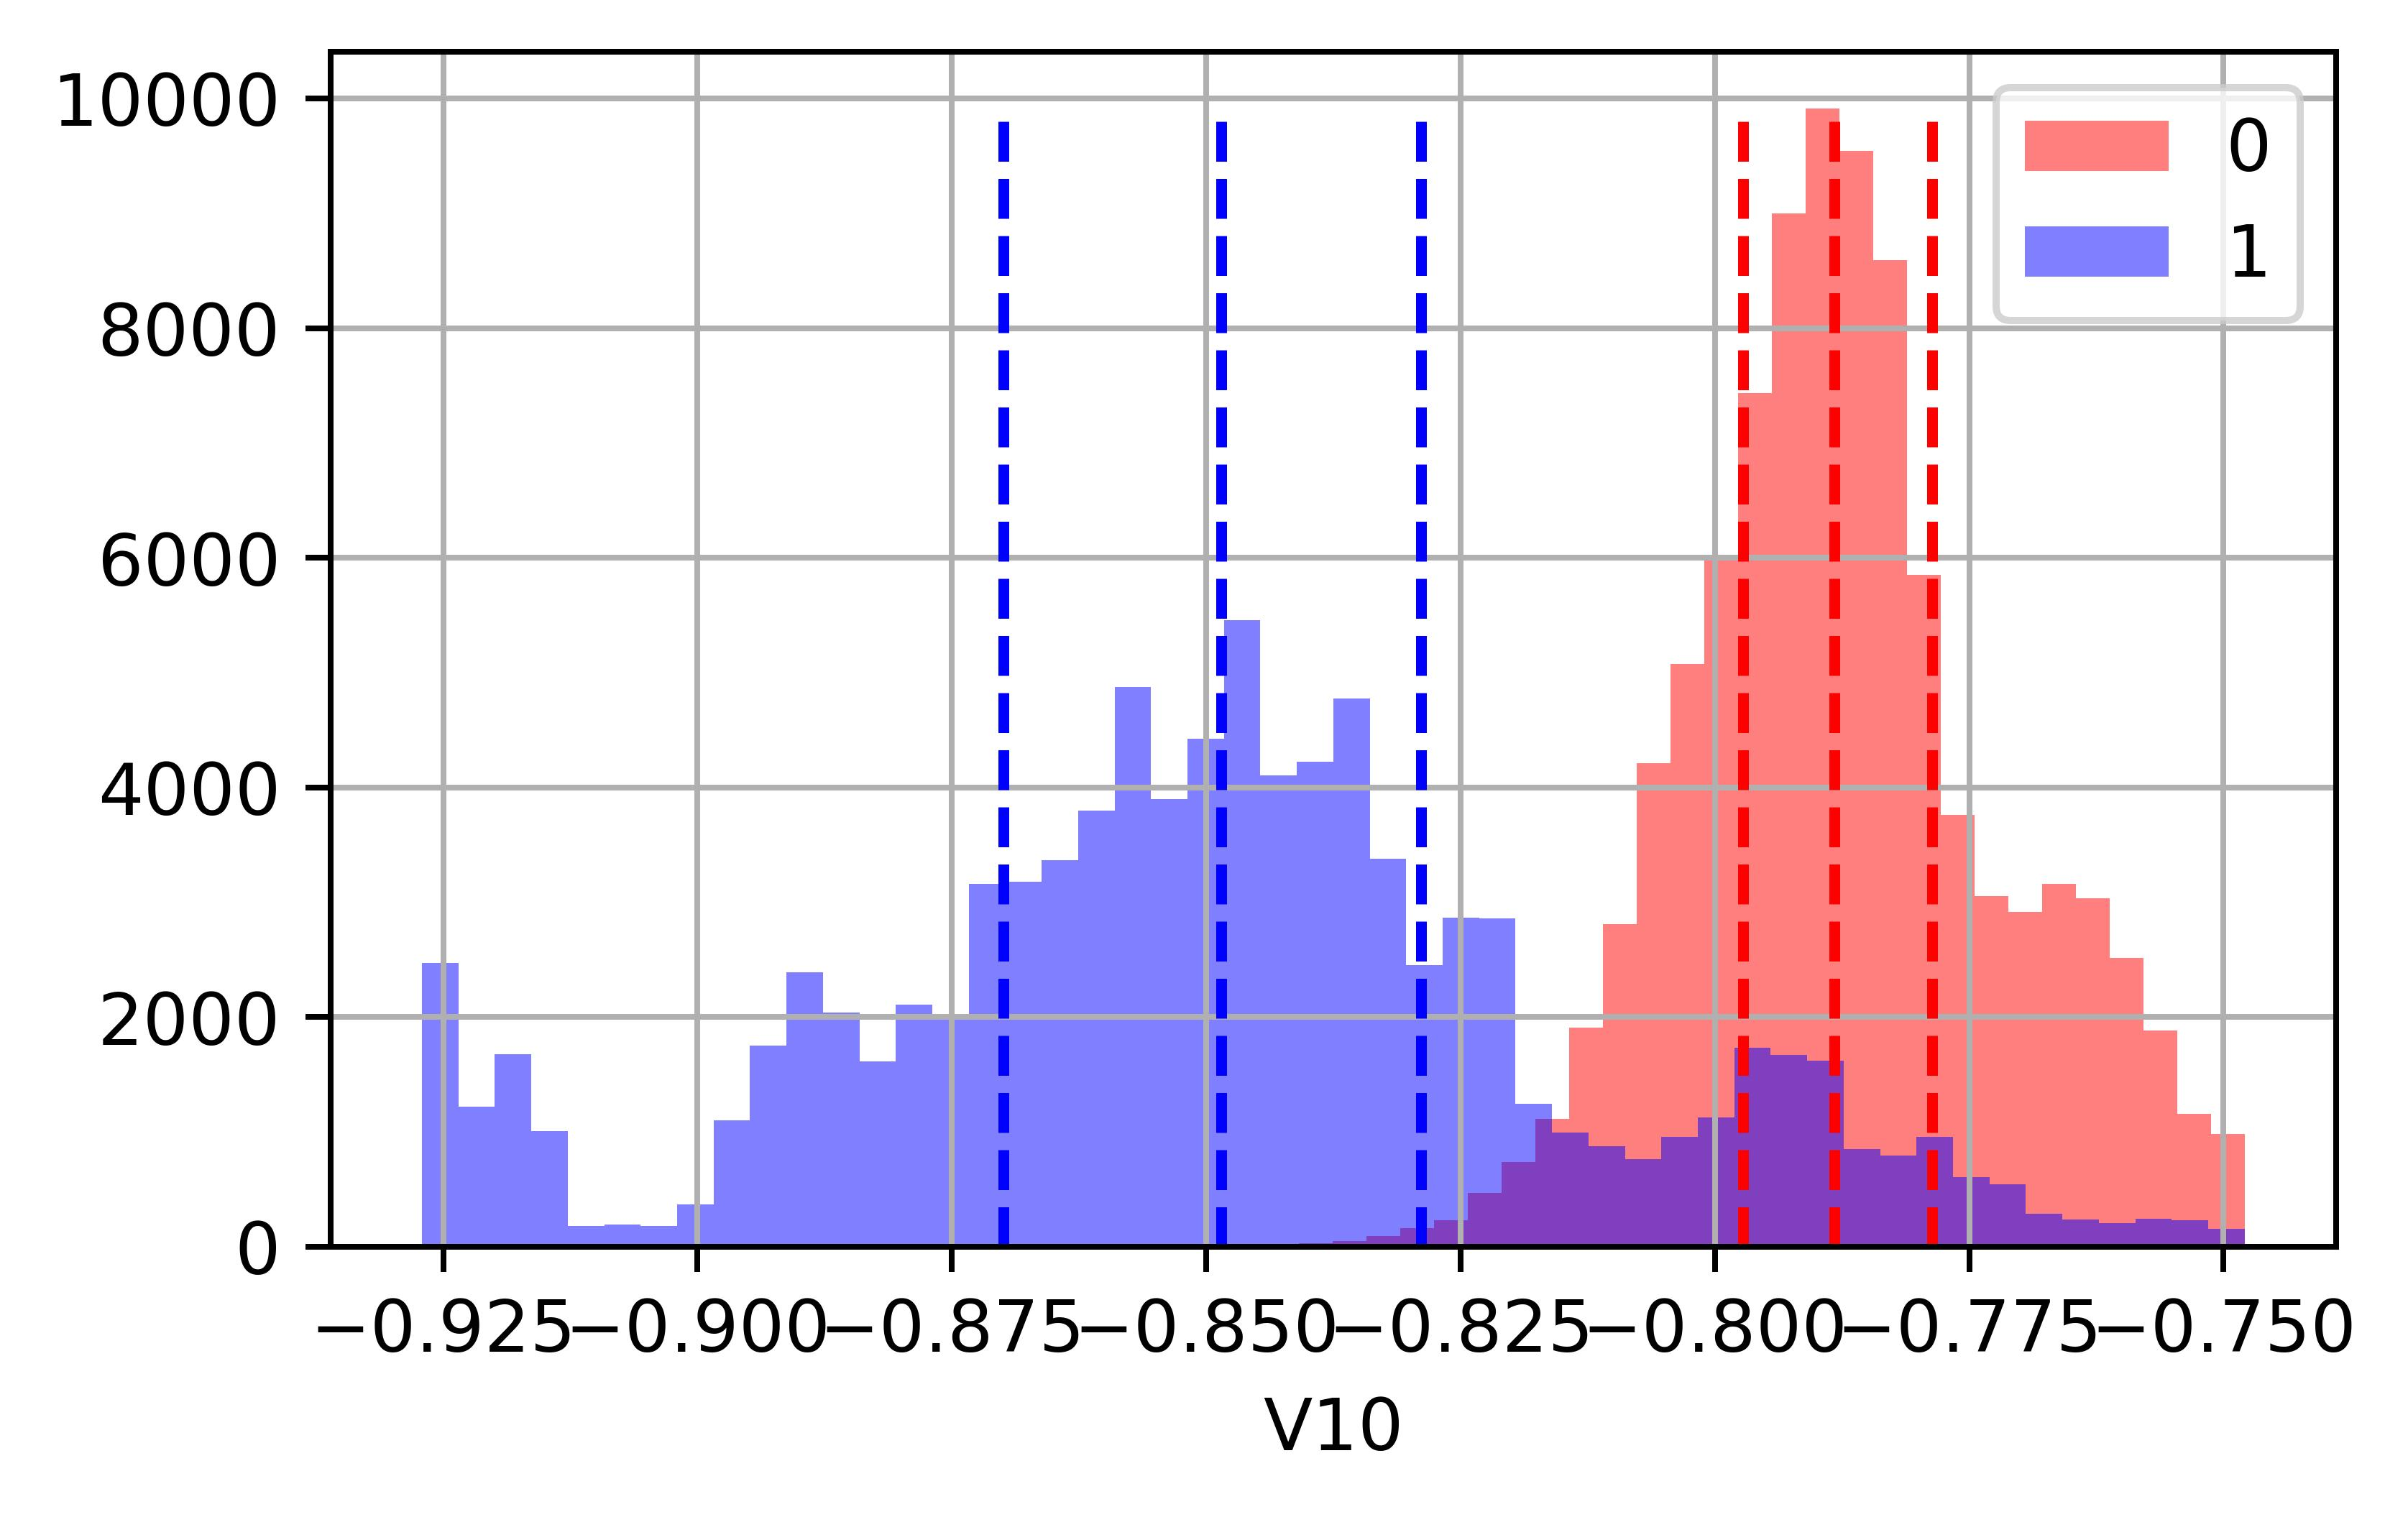
\includegraphics[width=0.18\textwidth]{../code/Task3/Analysis/Hist-V10.jpg} \\
  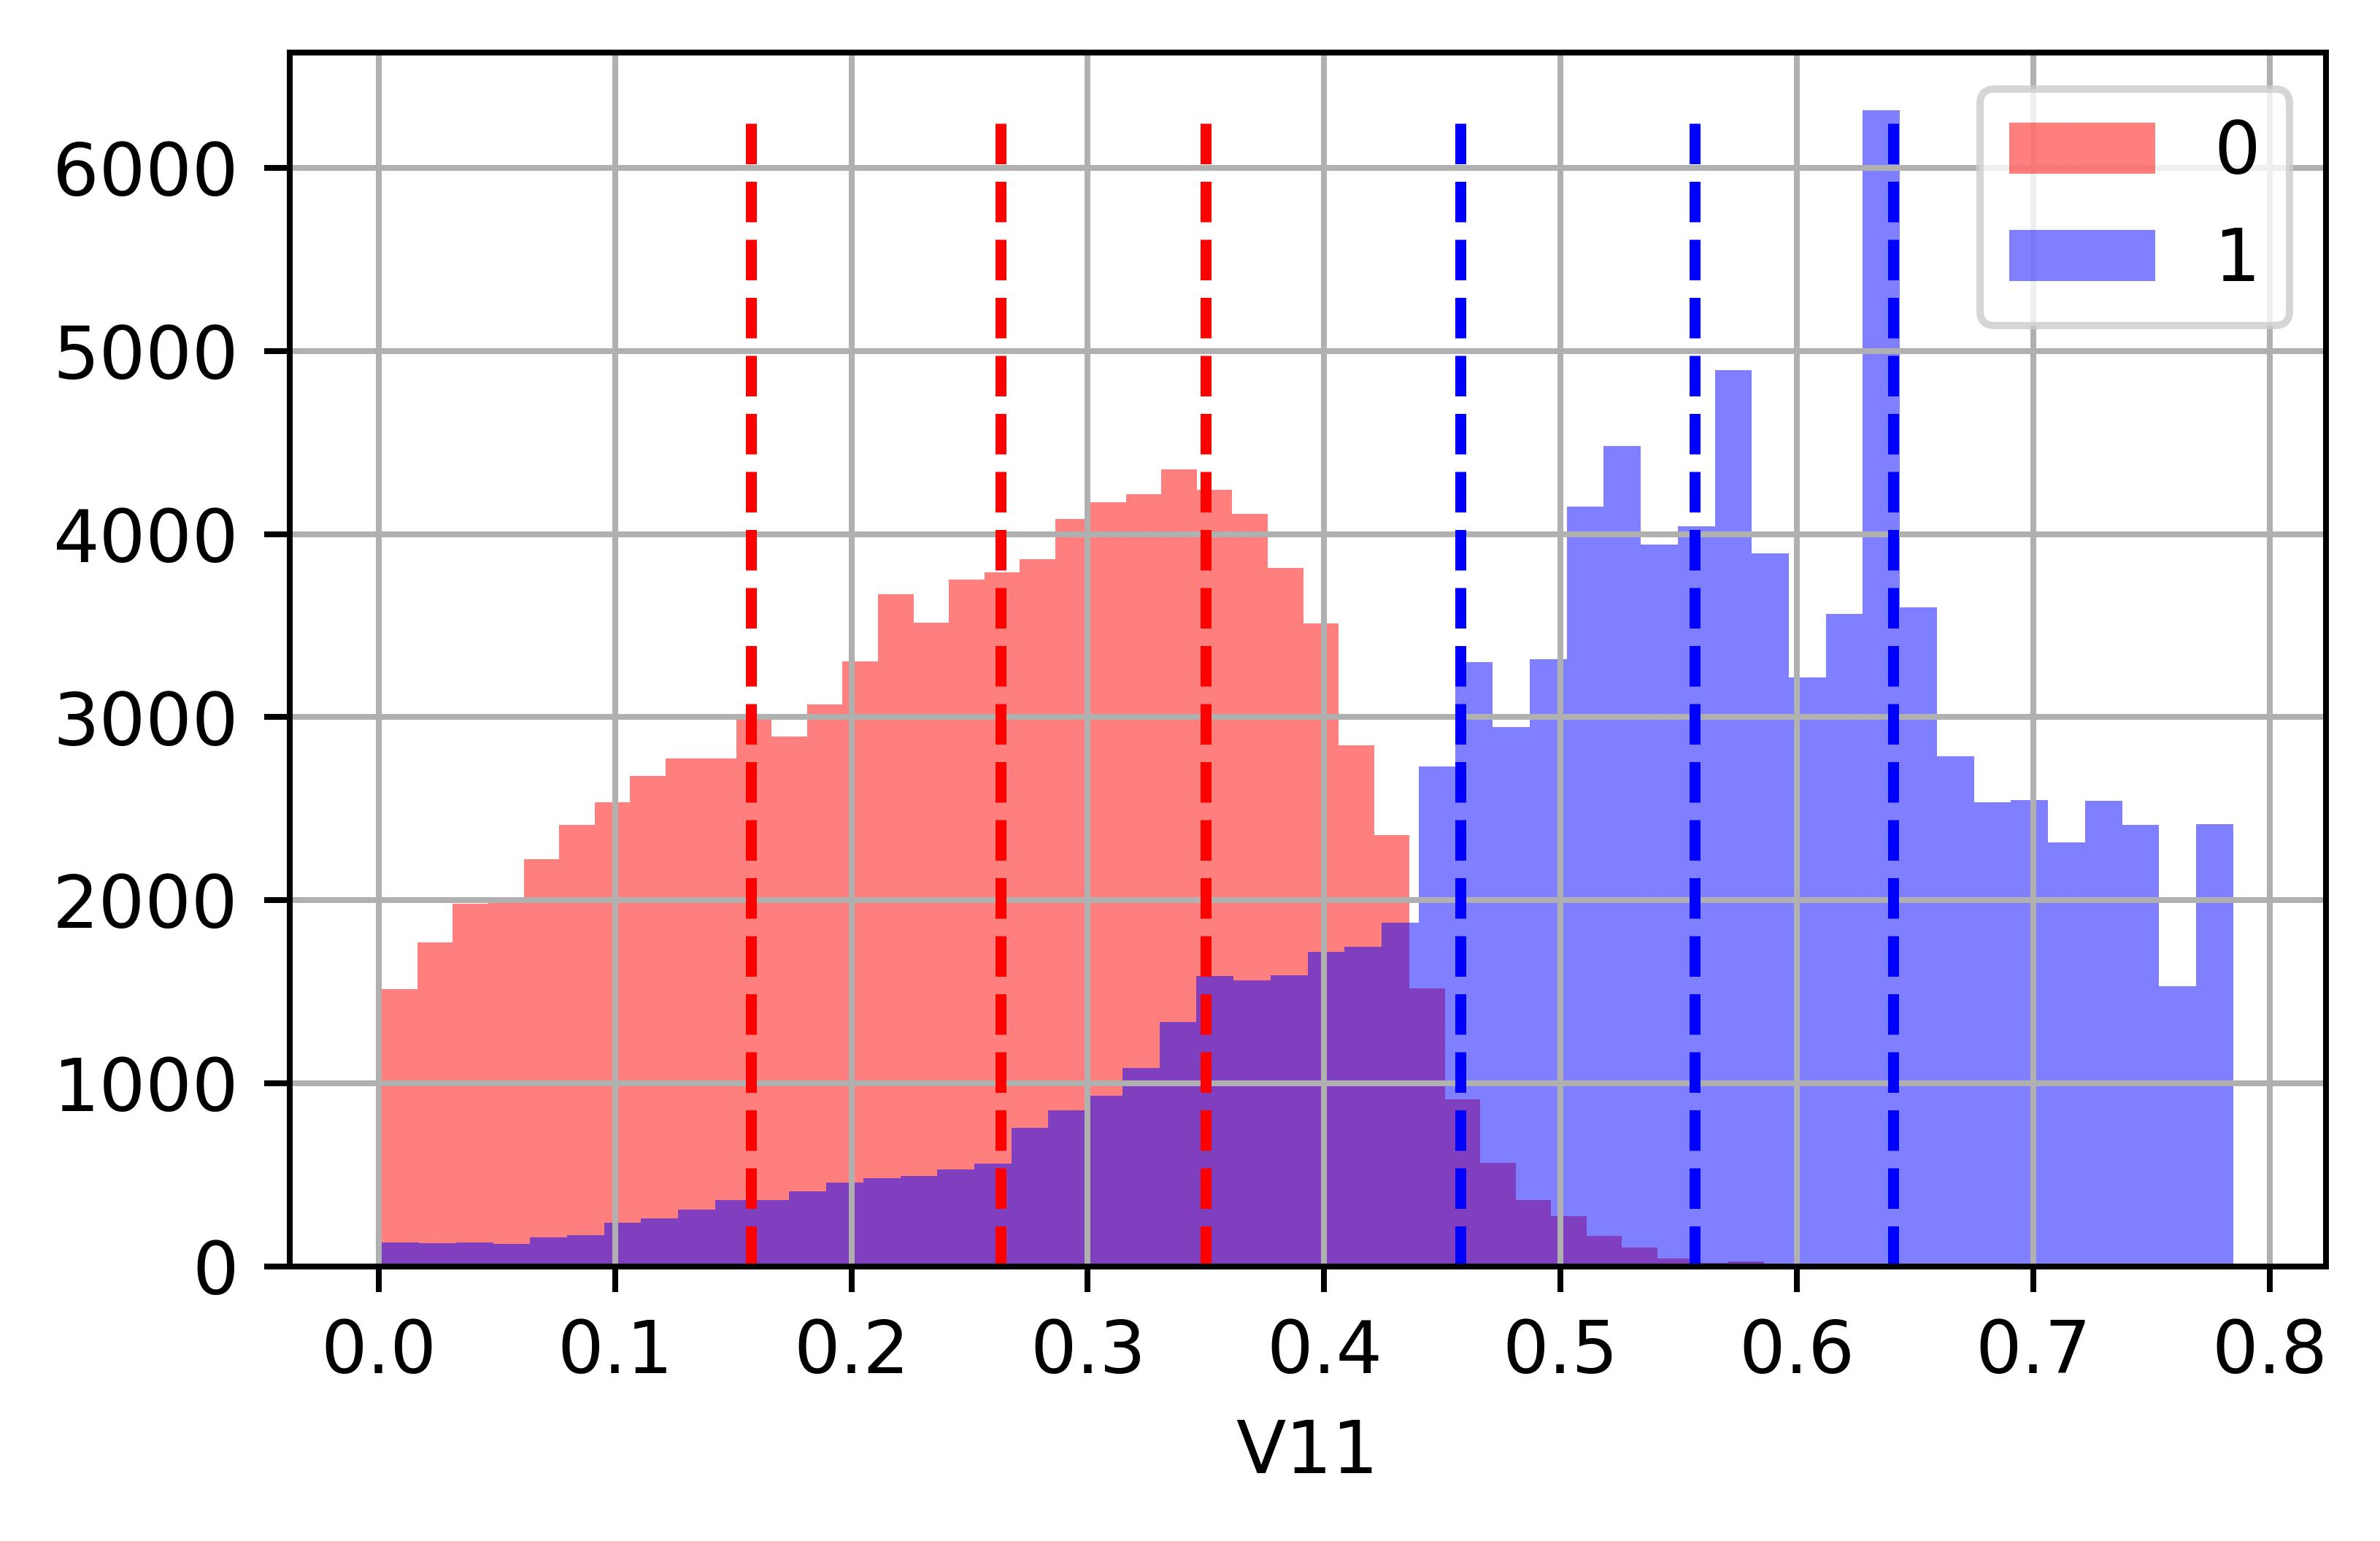
\includegraphics[width=0.18\textwidth]{../code/Task3/Analysis/Hist-V11.jpg}
  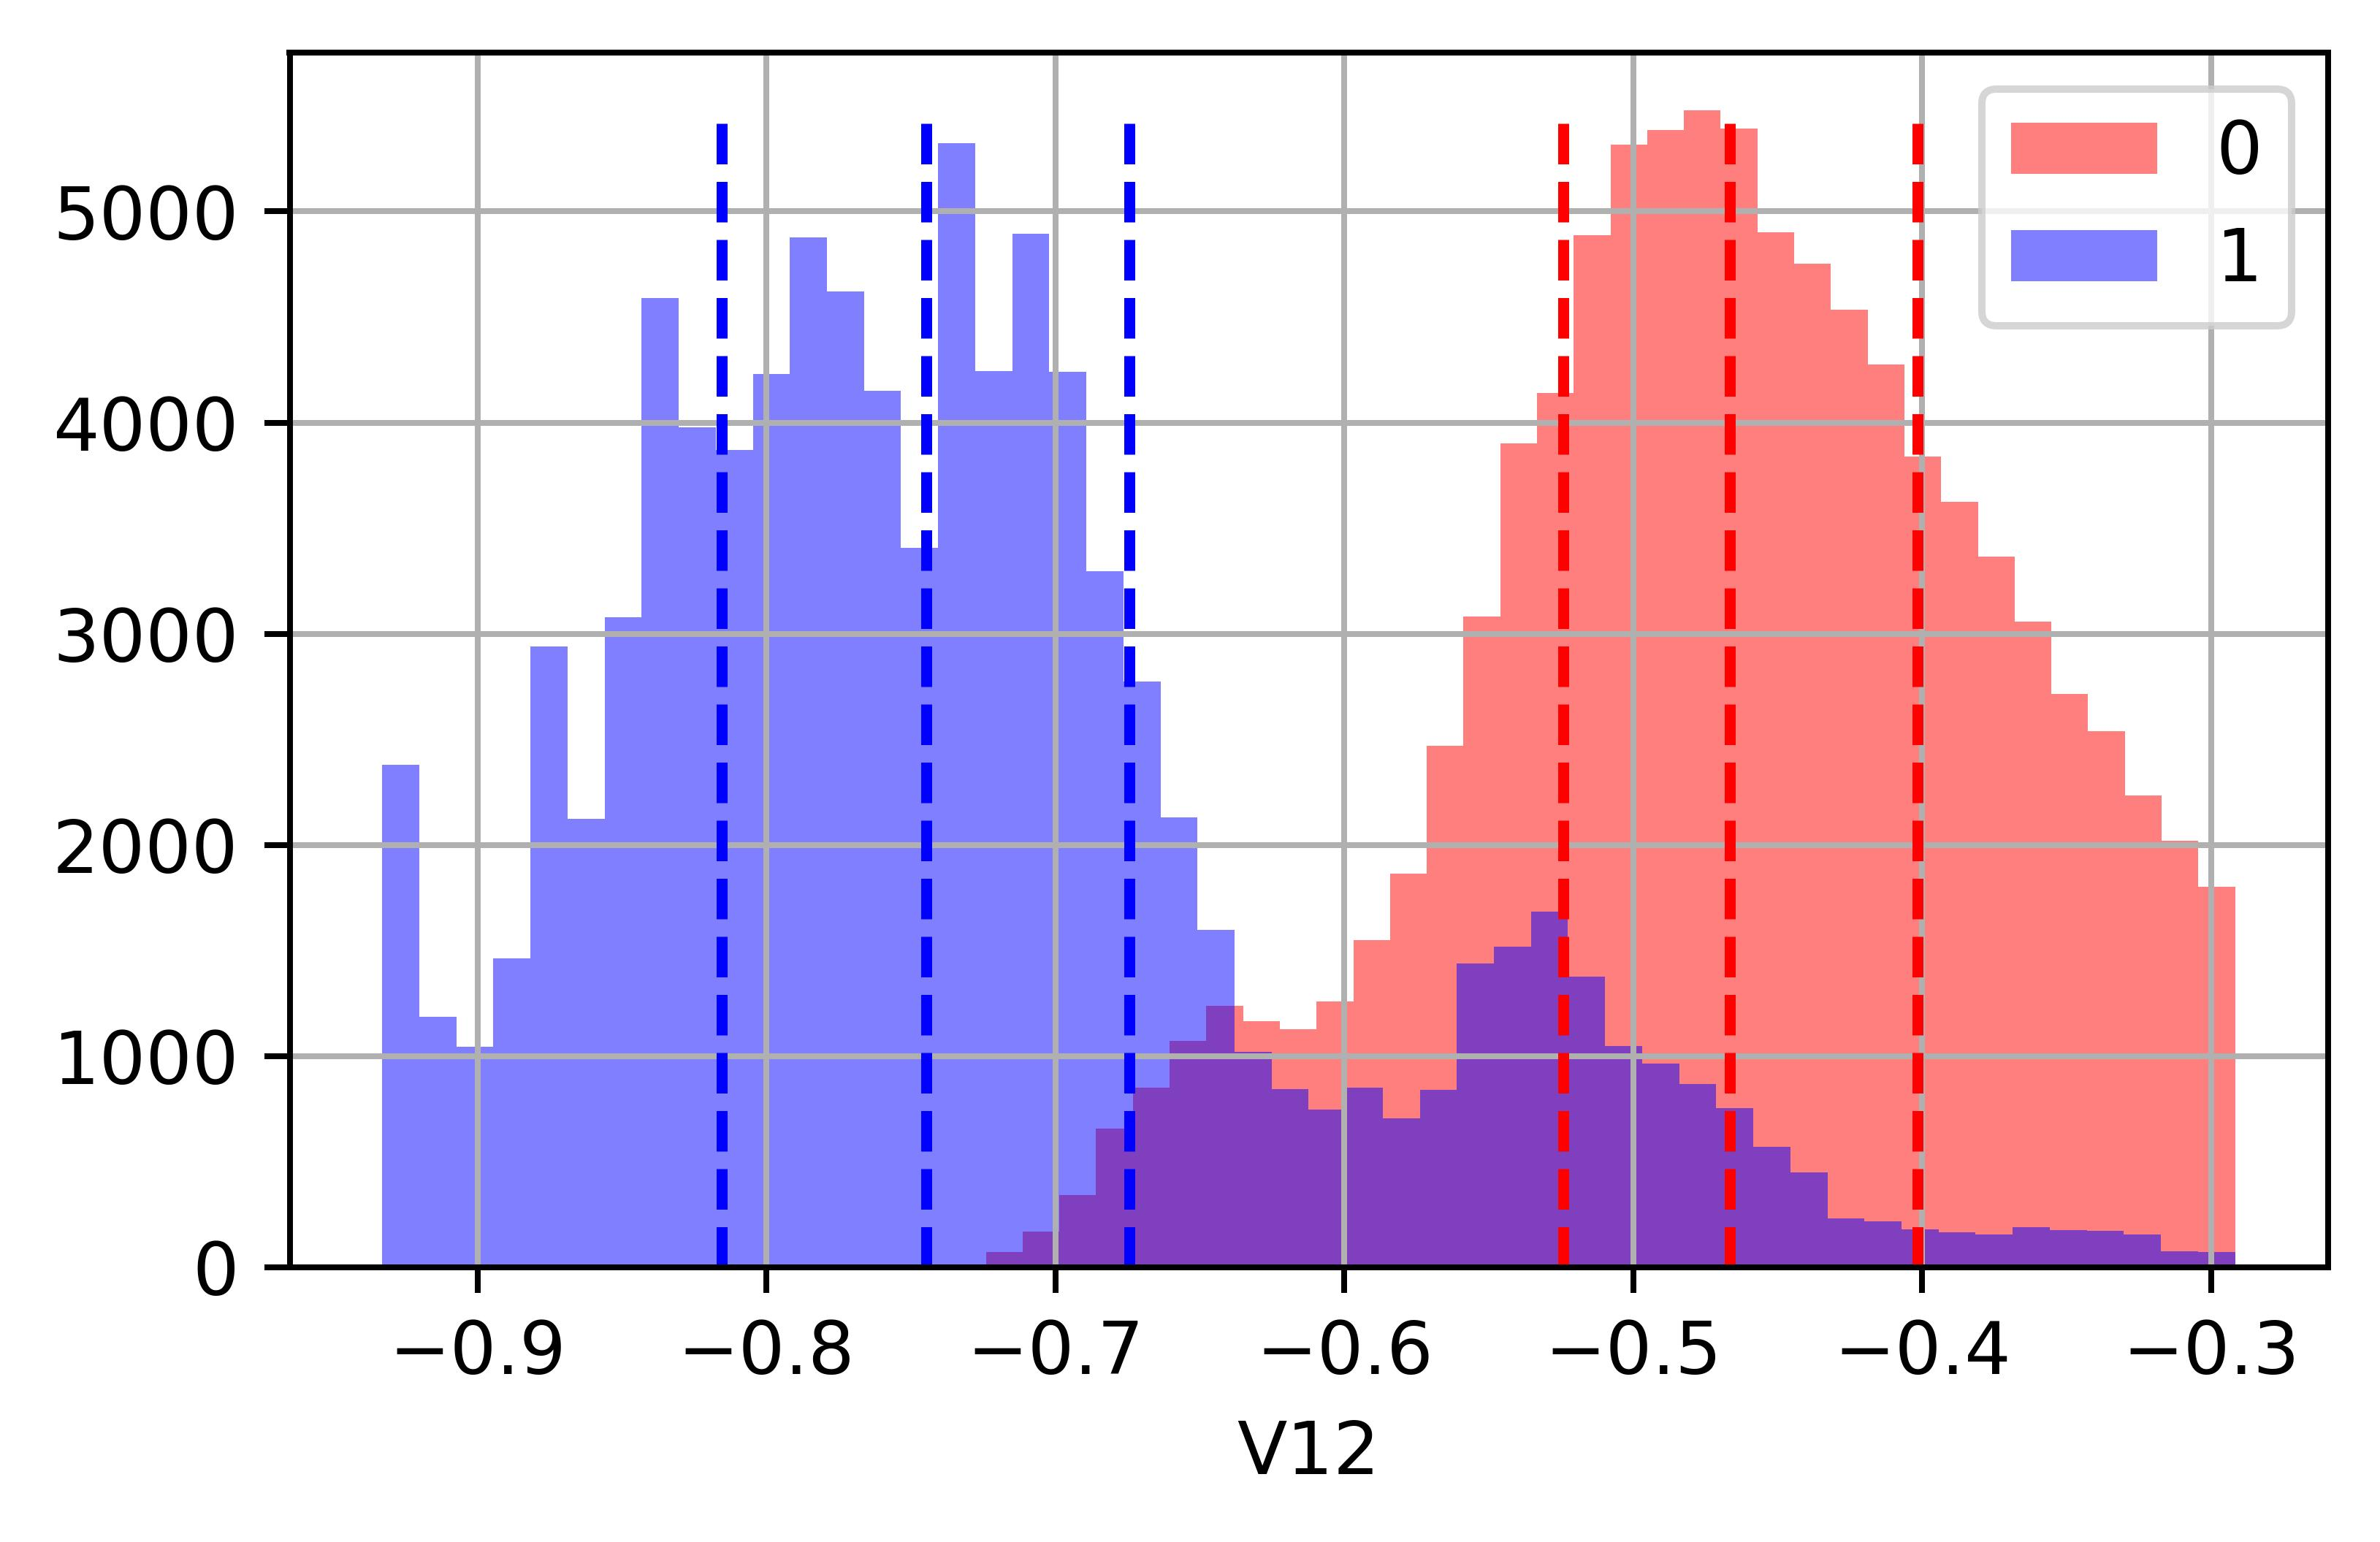
\includegraphics[width=0.18\textwidth]{../code/Task3/Analysis/Hist-V12.jpg}
  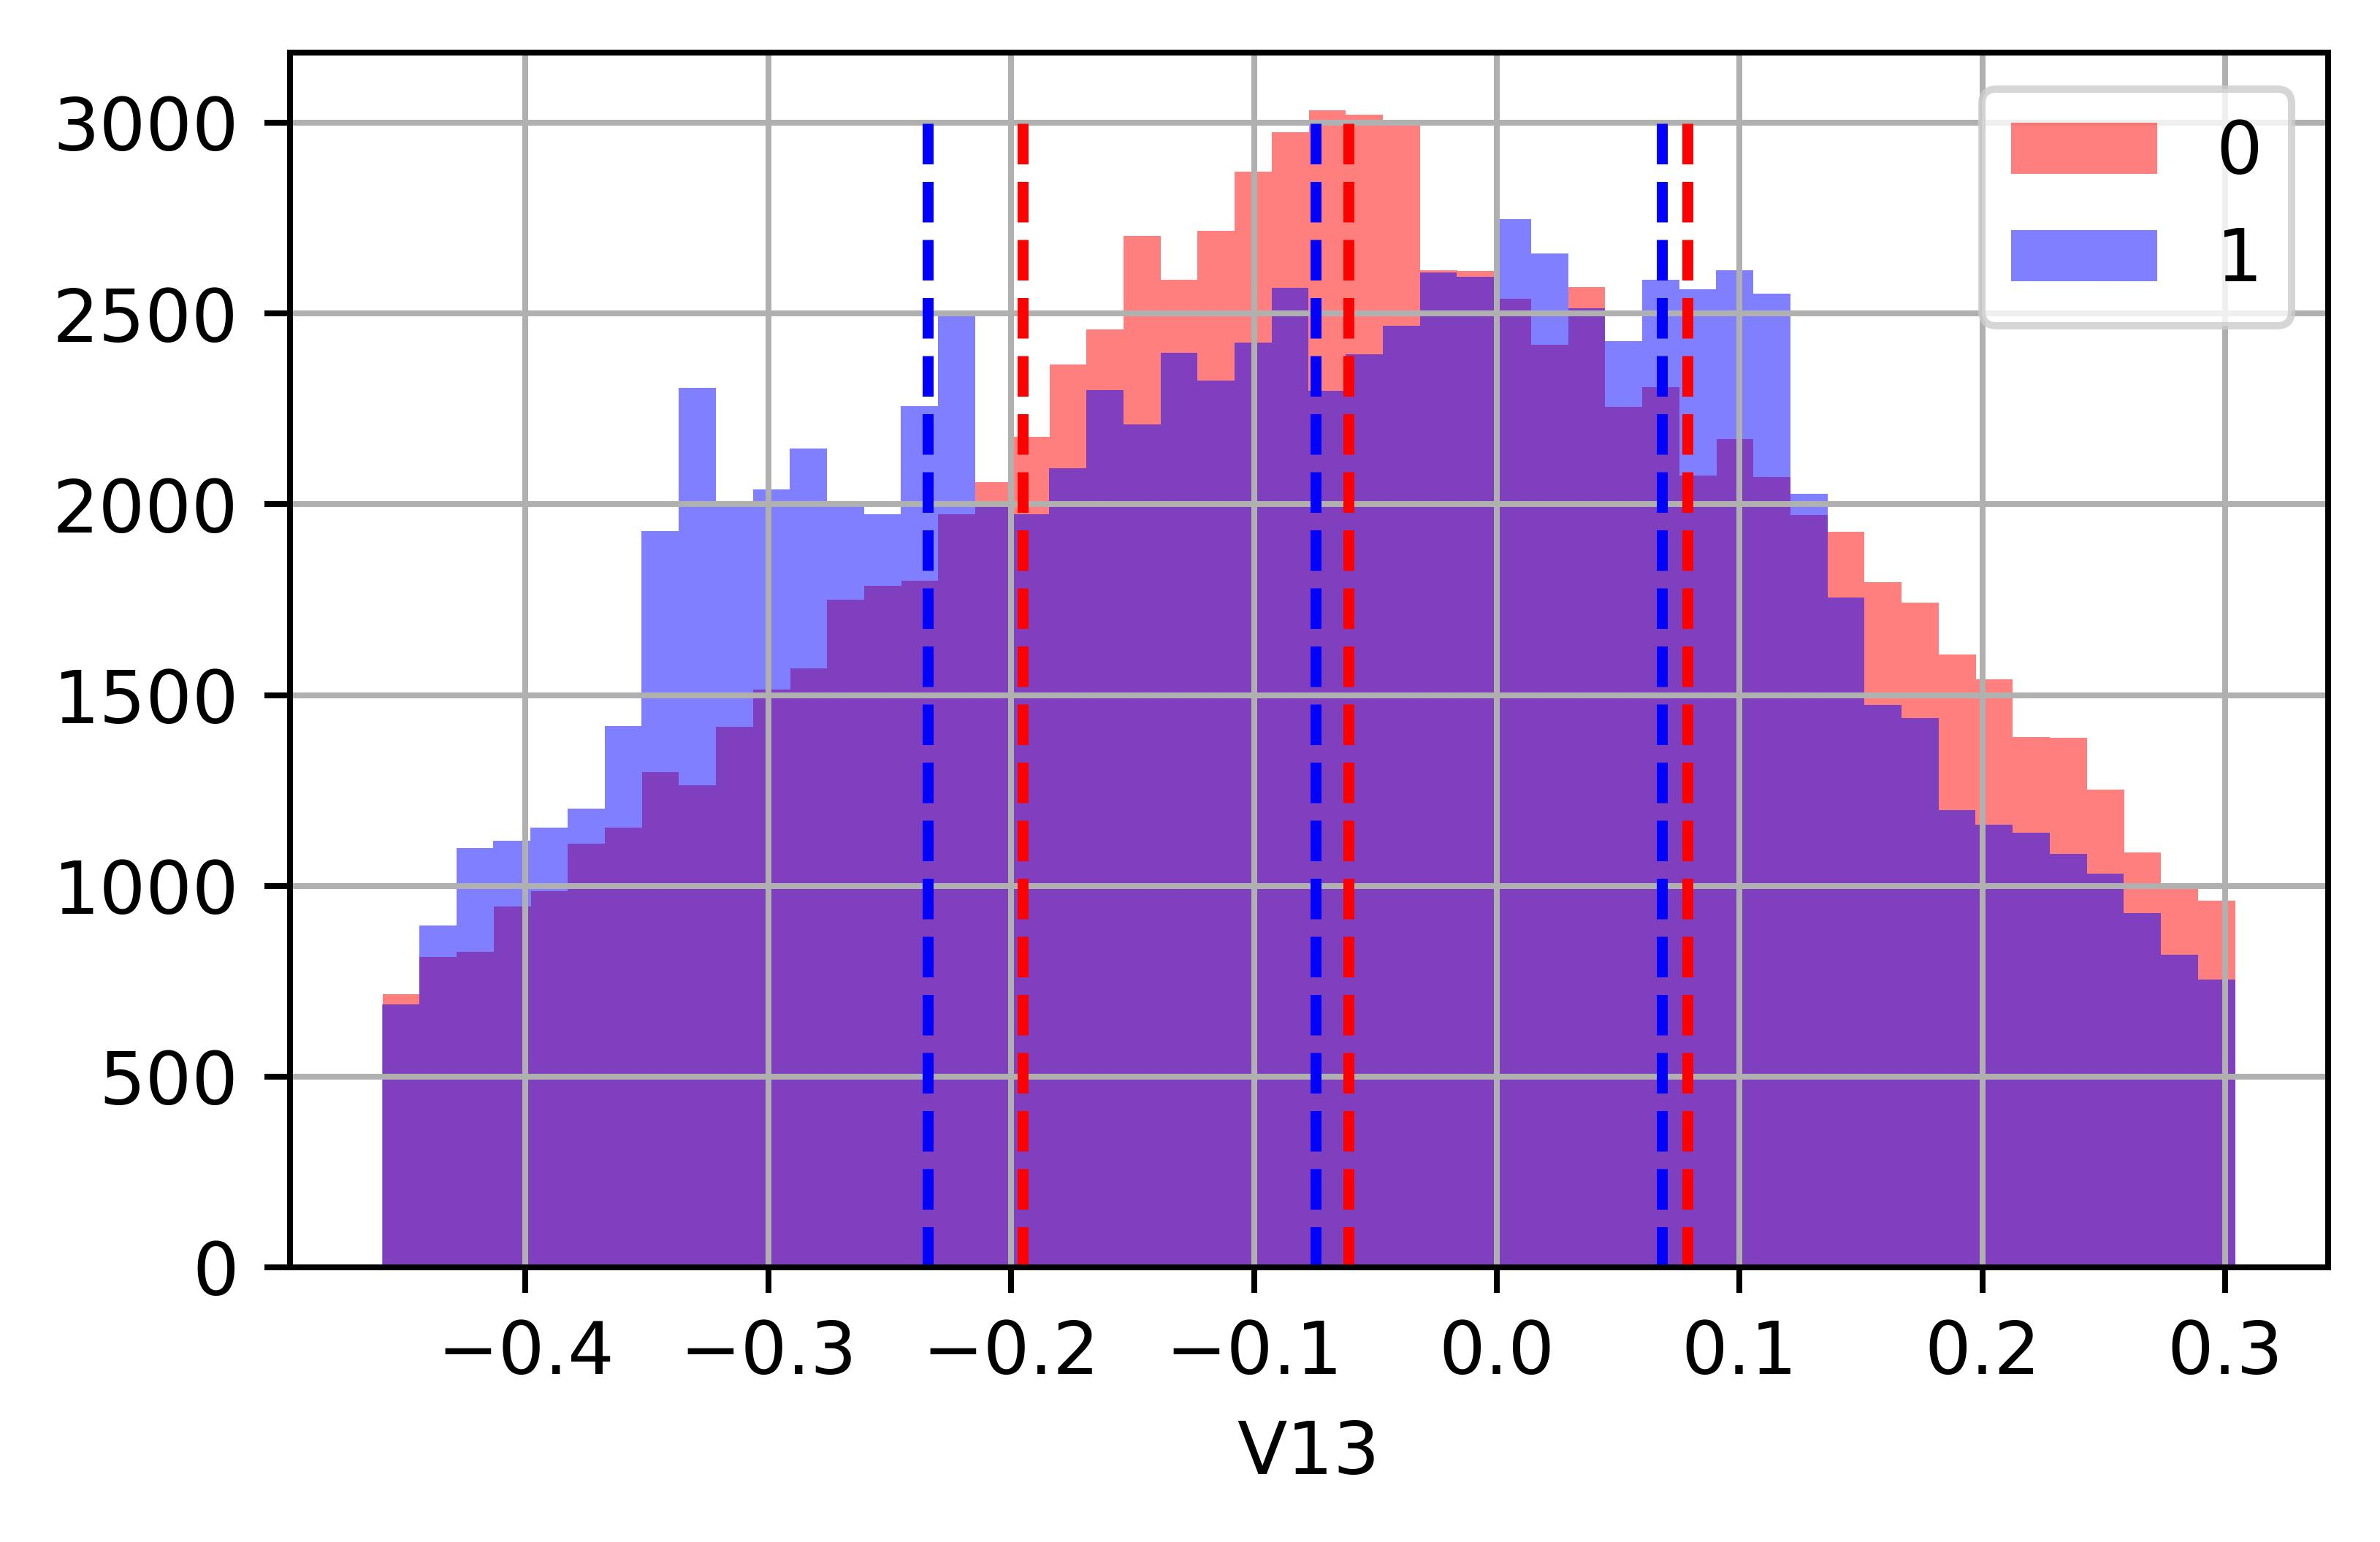
\includegraphics[width=0.18\textwidth]{../code/Task3/Analysis/Hist-V13.jpg}
  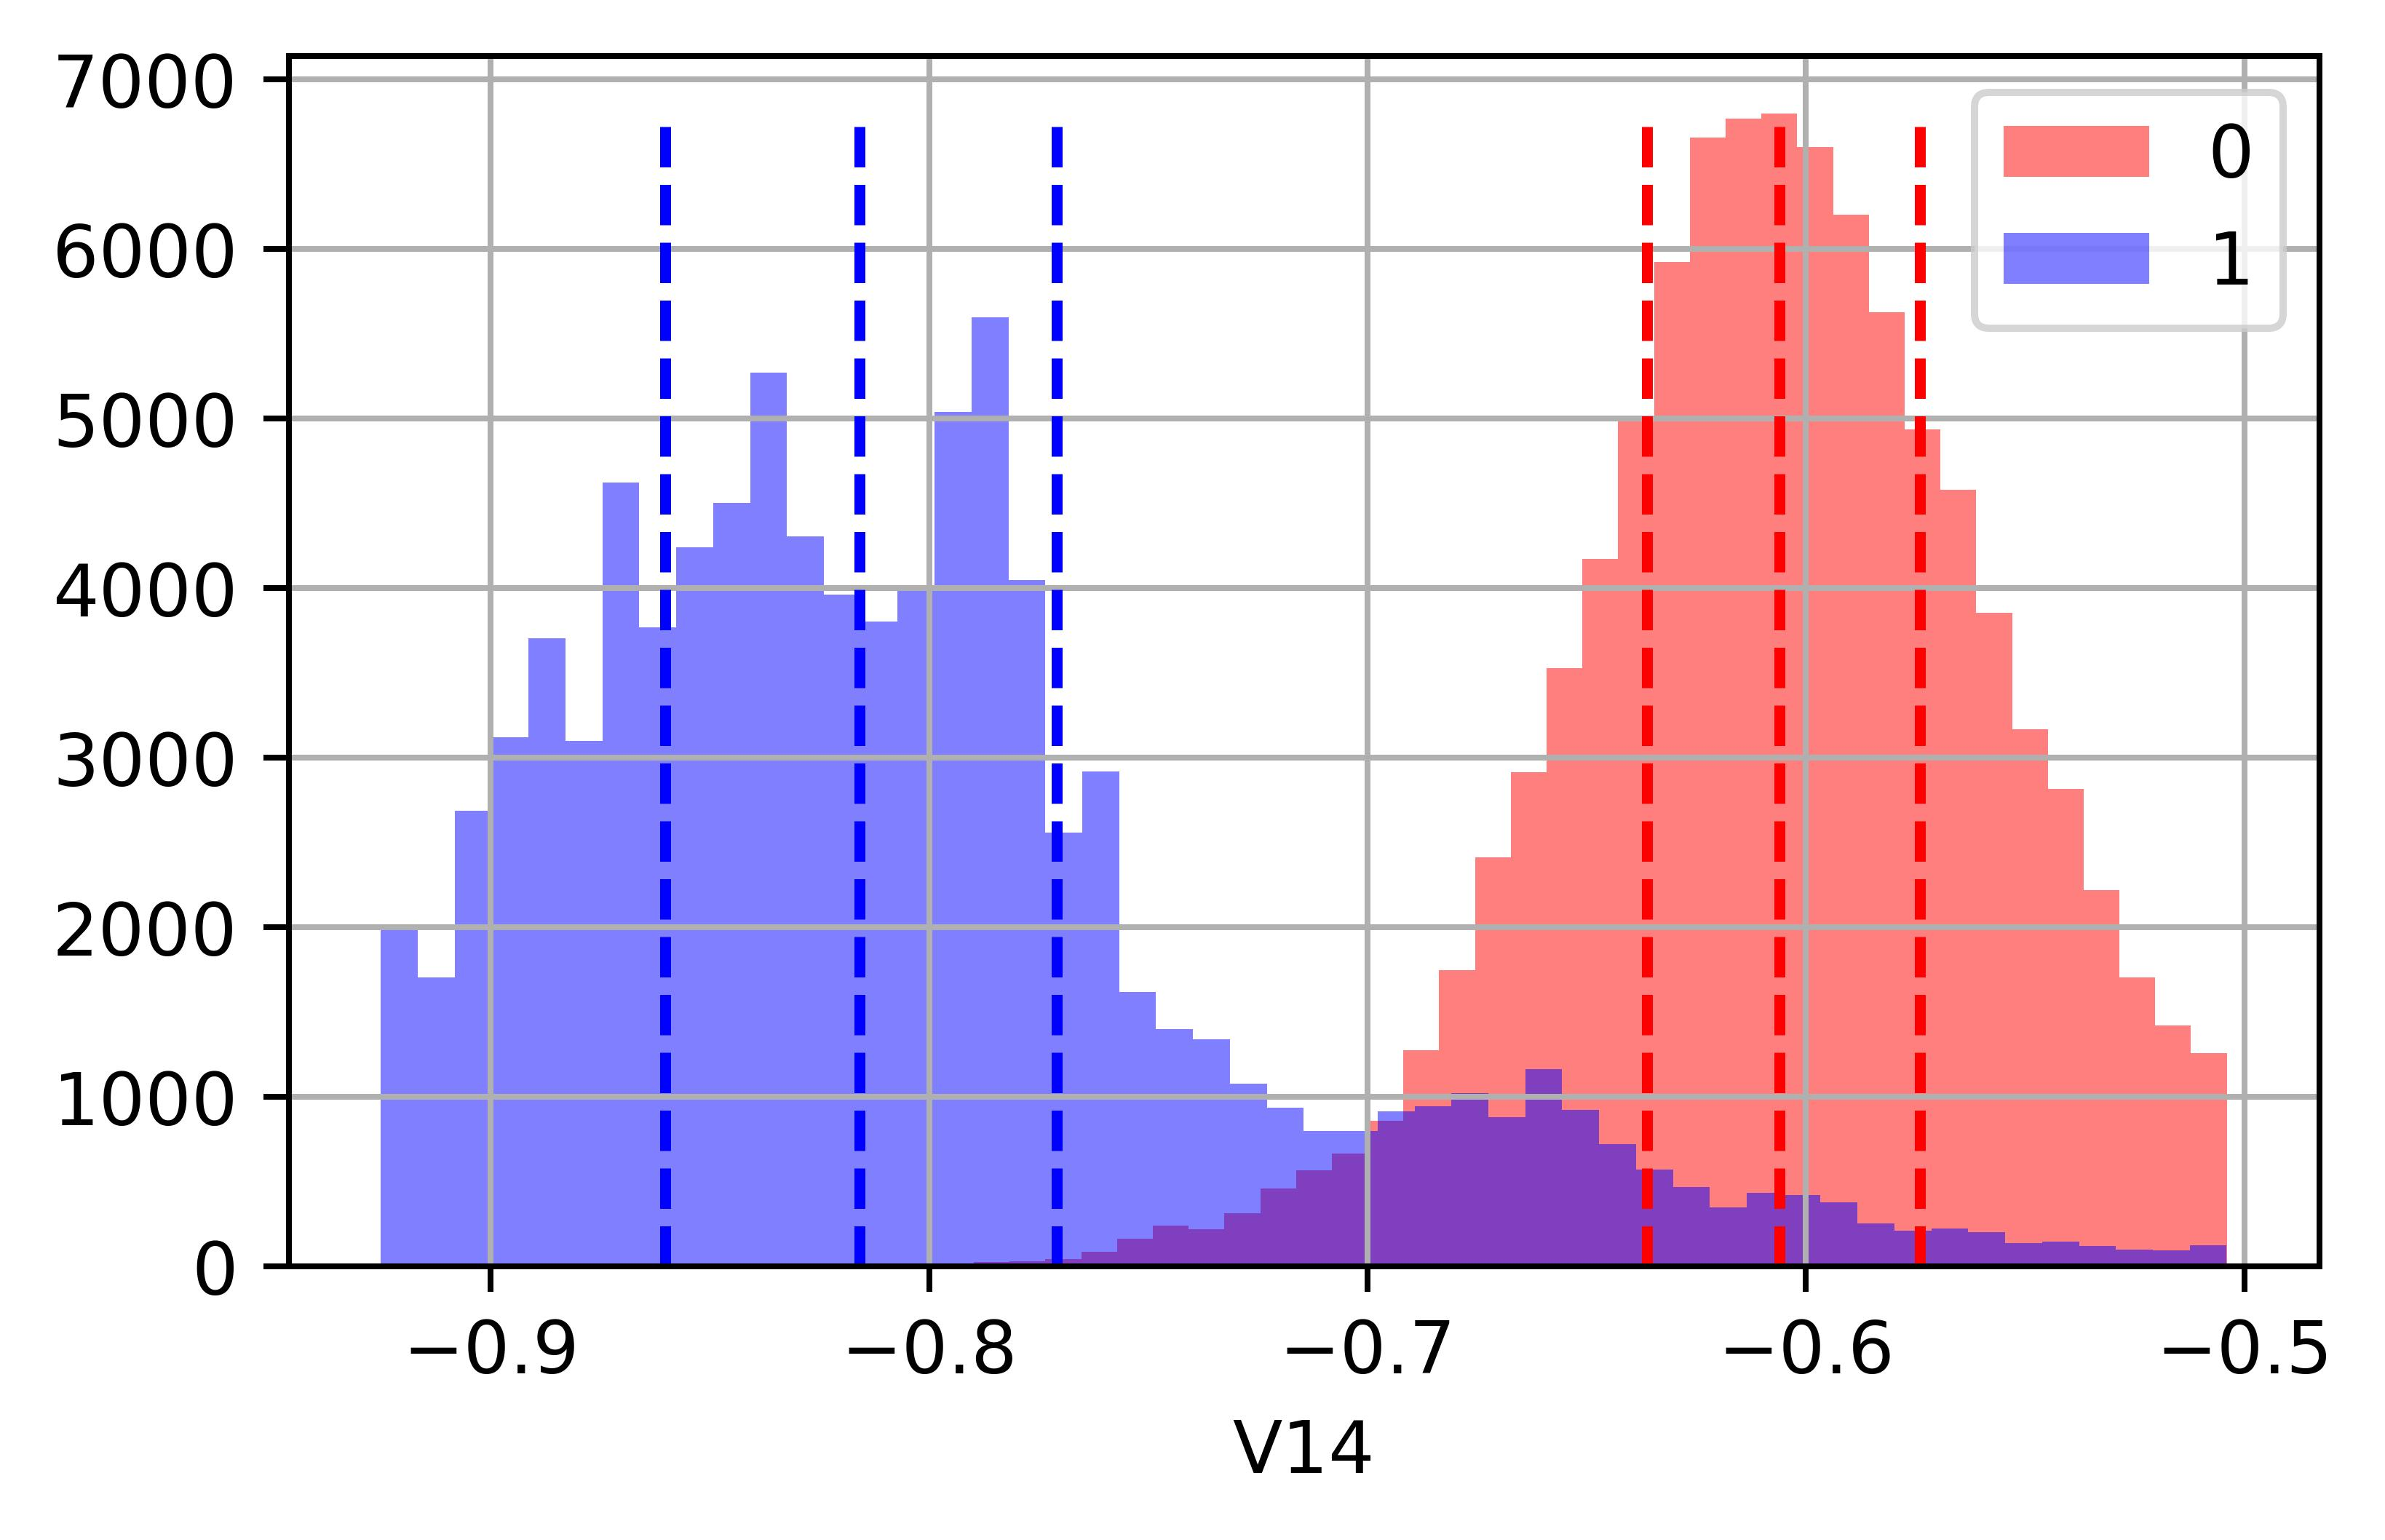
\includegraphics[width=0.18\textwidth]{../code/Task3/Analysis/Hist-V14.jpg}
  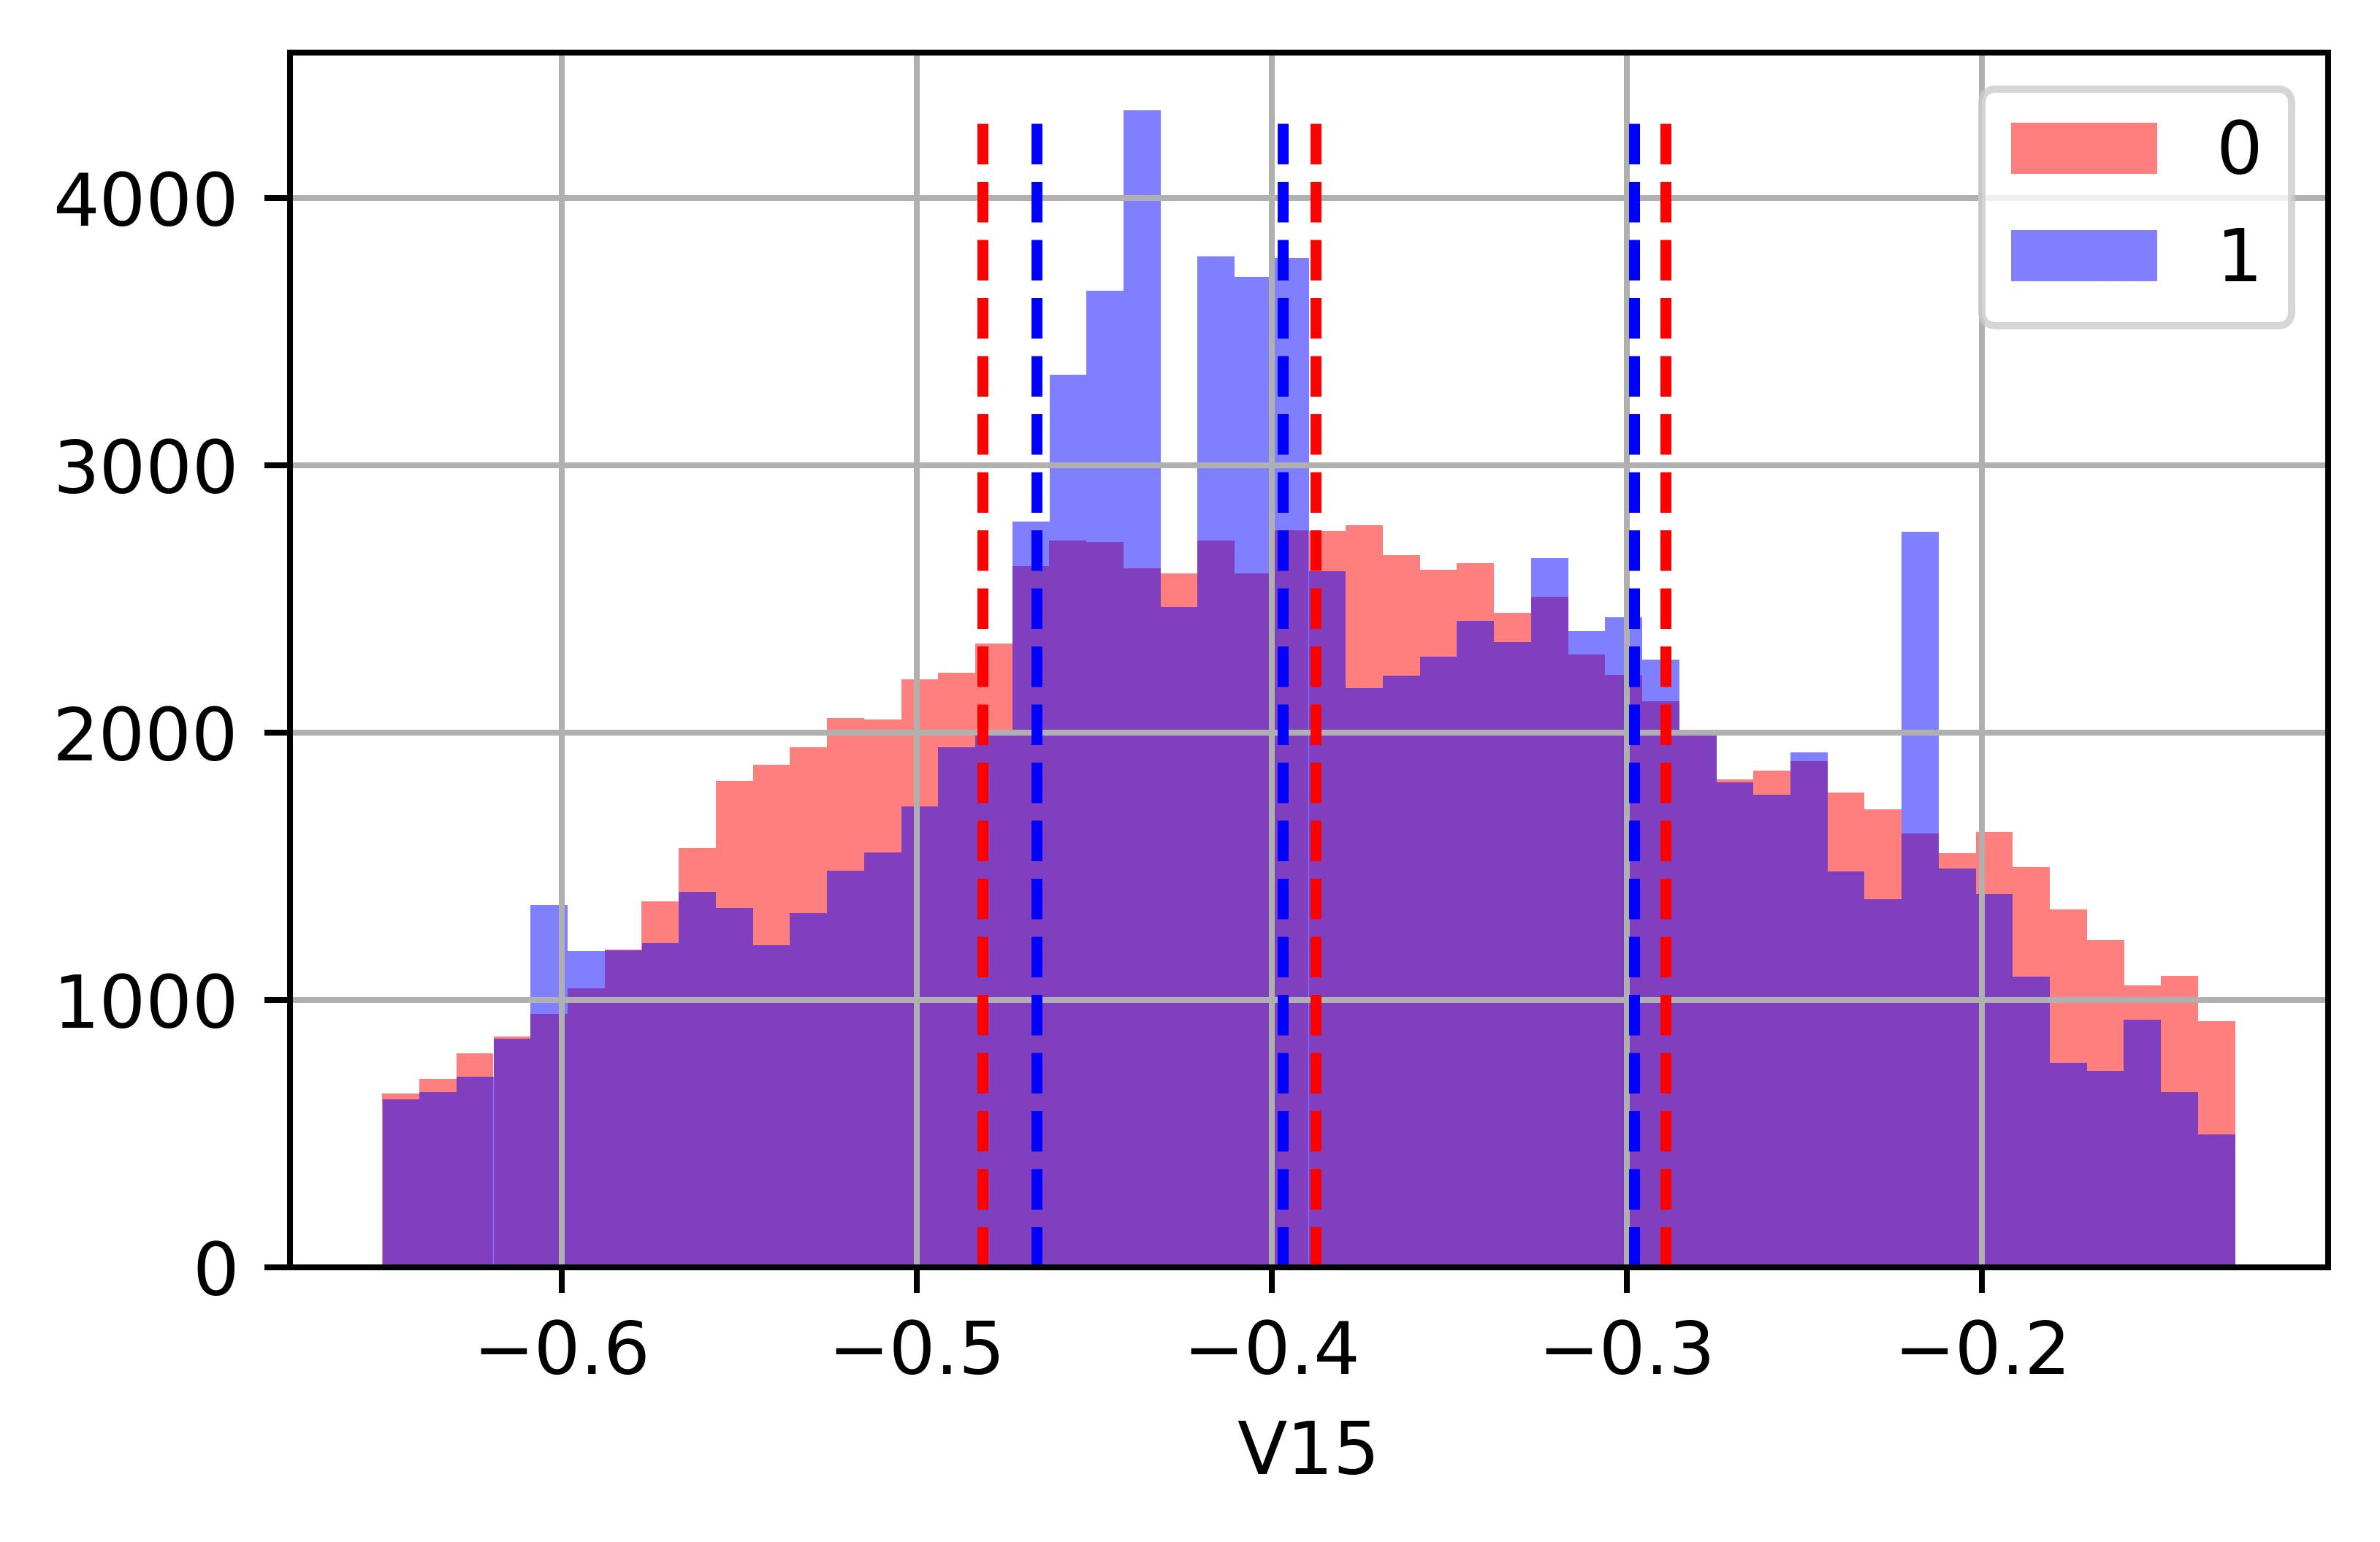
\includegraphics[width=0.18\textwidth]{../code/Task3/Analysis/Hist-V15.jpg} \\
  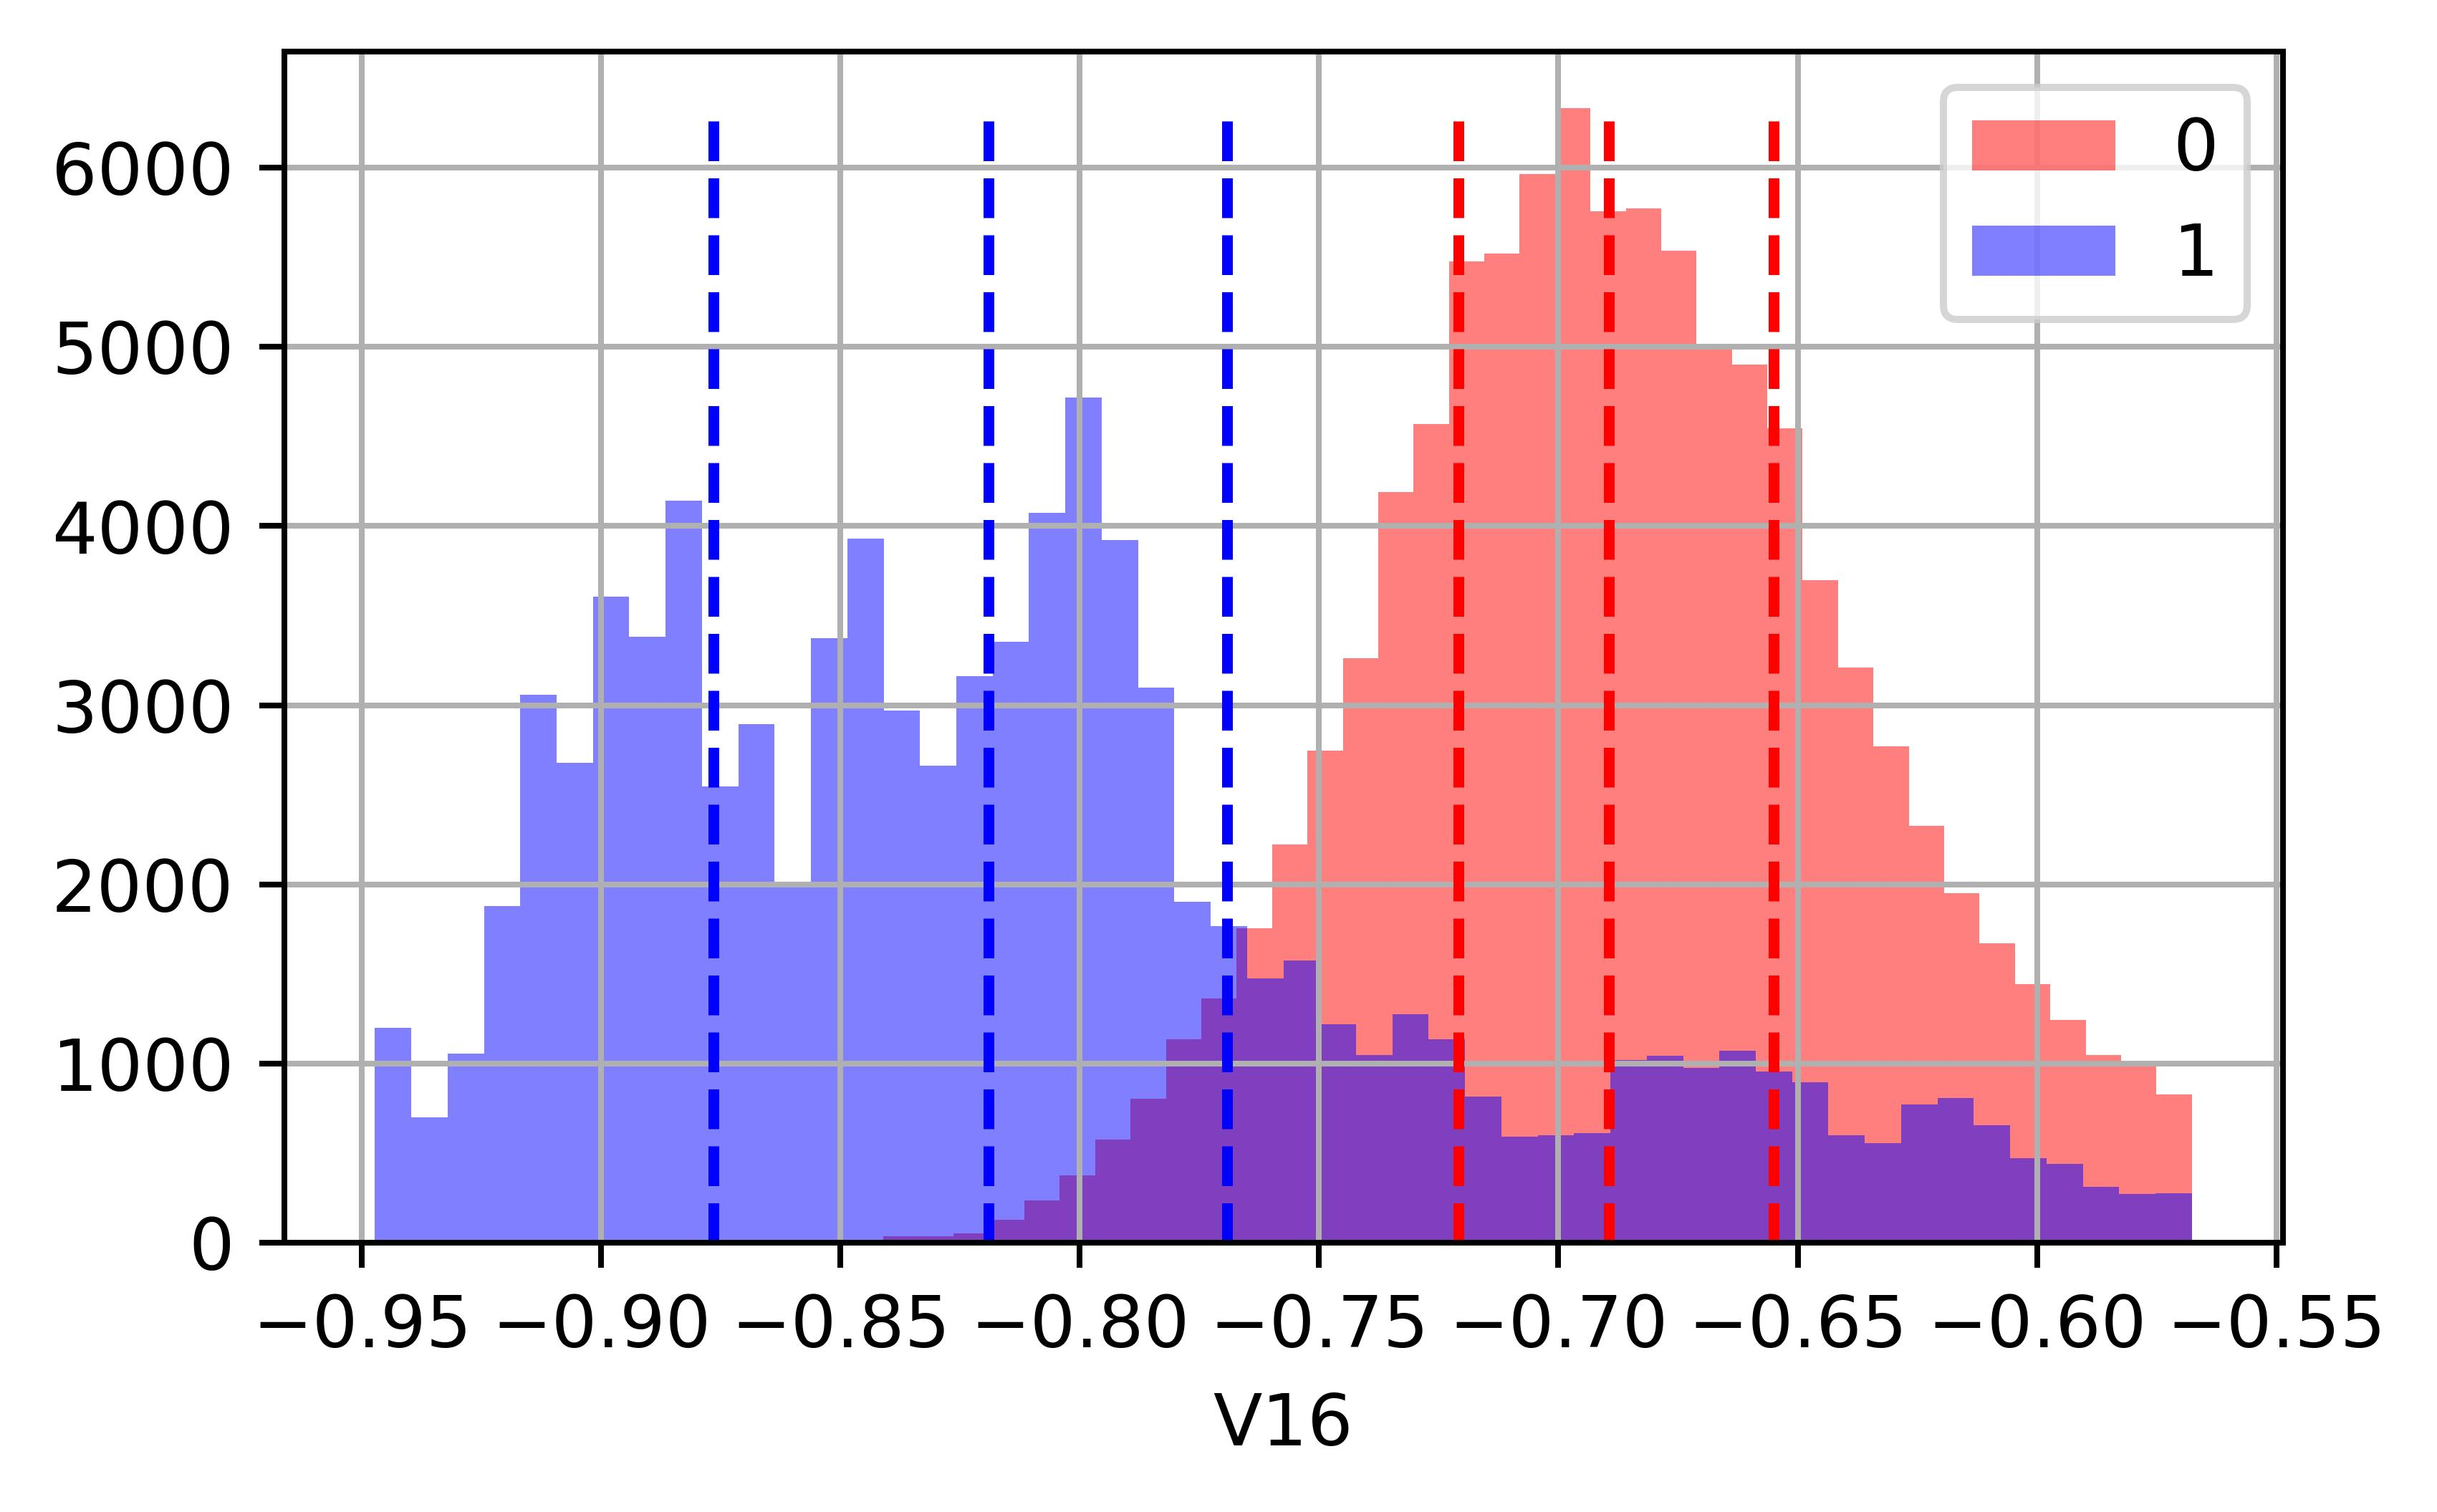
\includegraphics[width=0.18\textwidth]{../code/Task3/Analysis/Hist-V16.jpg}
  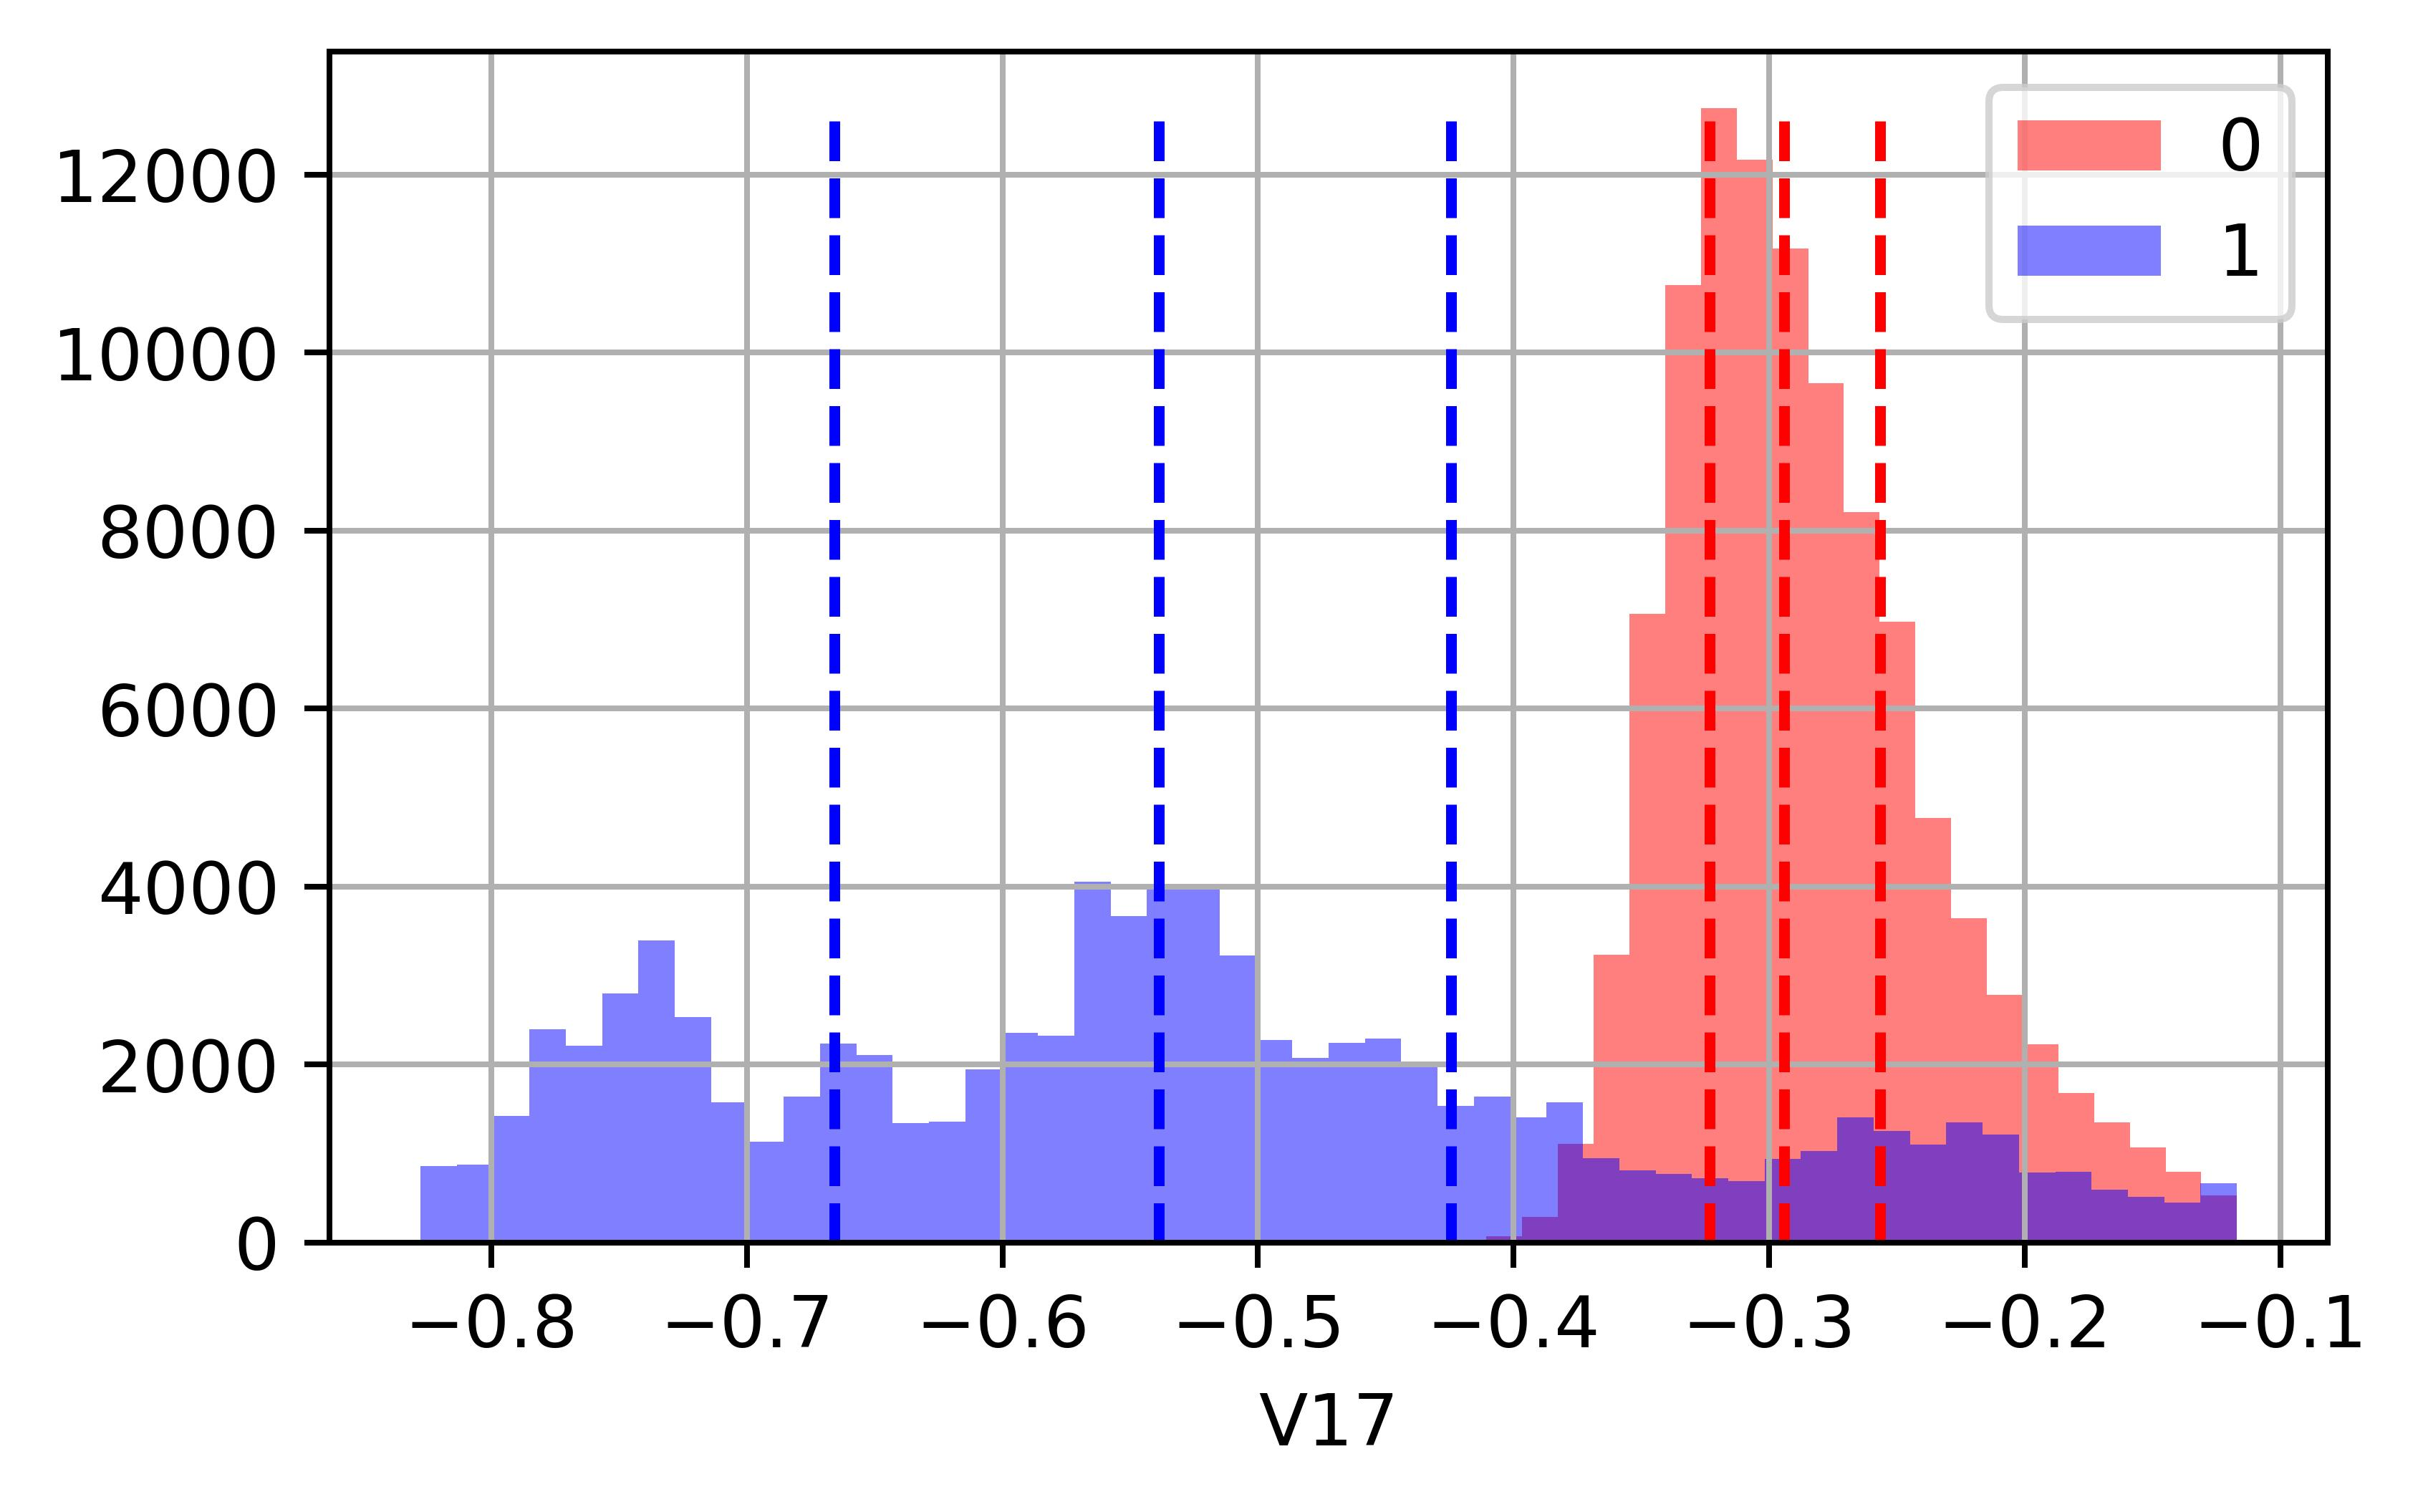
\includegraphics[width=0.18\textwidth]{../code/Task3/Analysis/Hist-V17.jpg}
  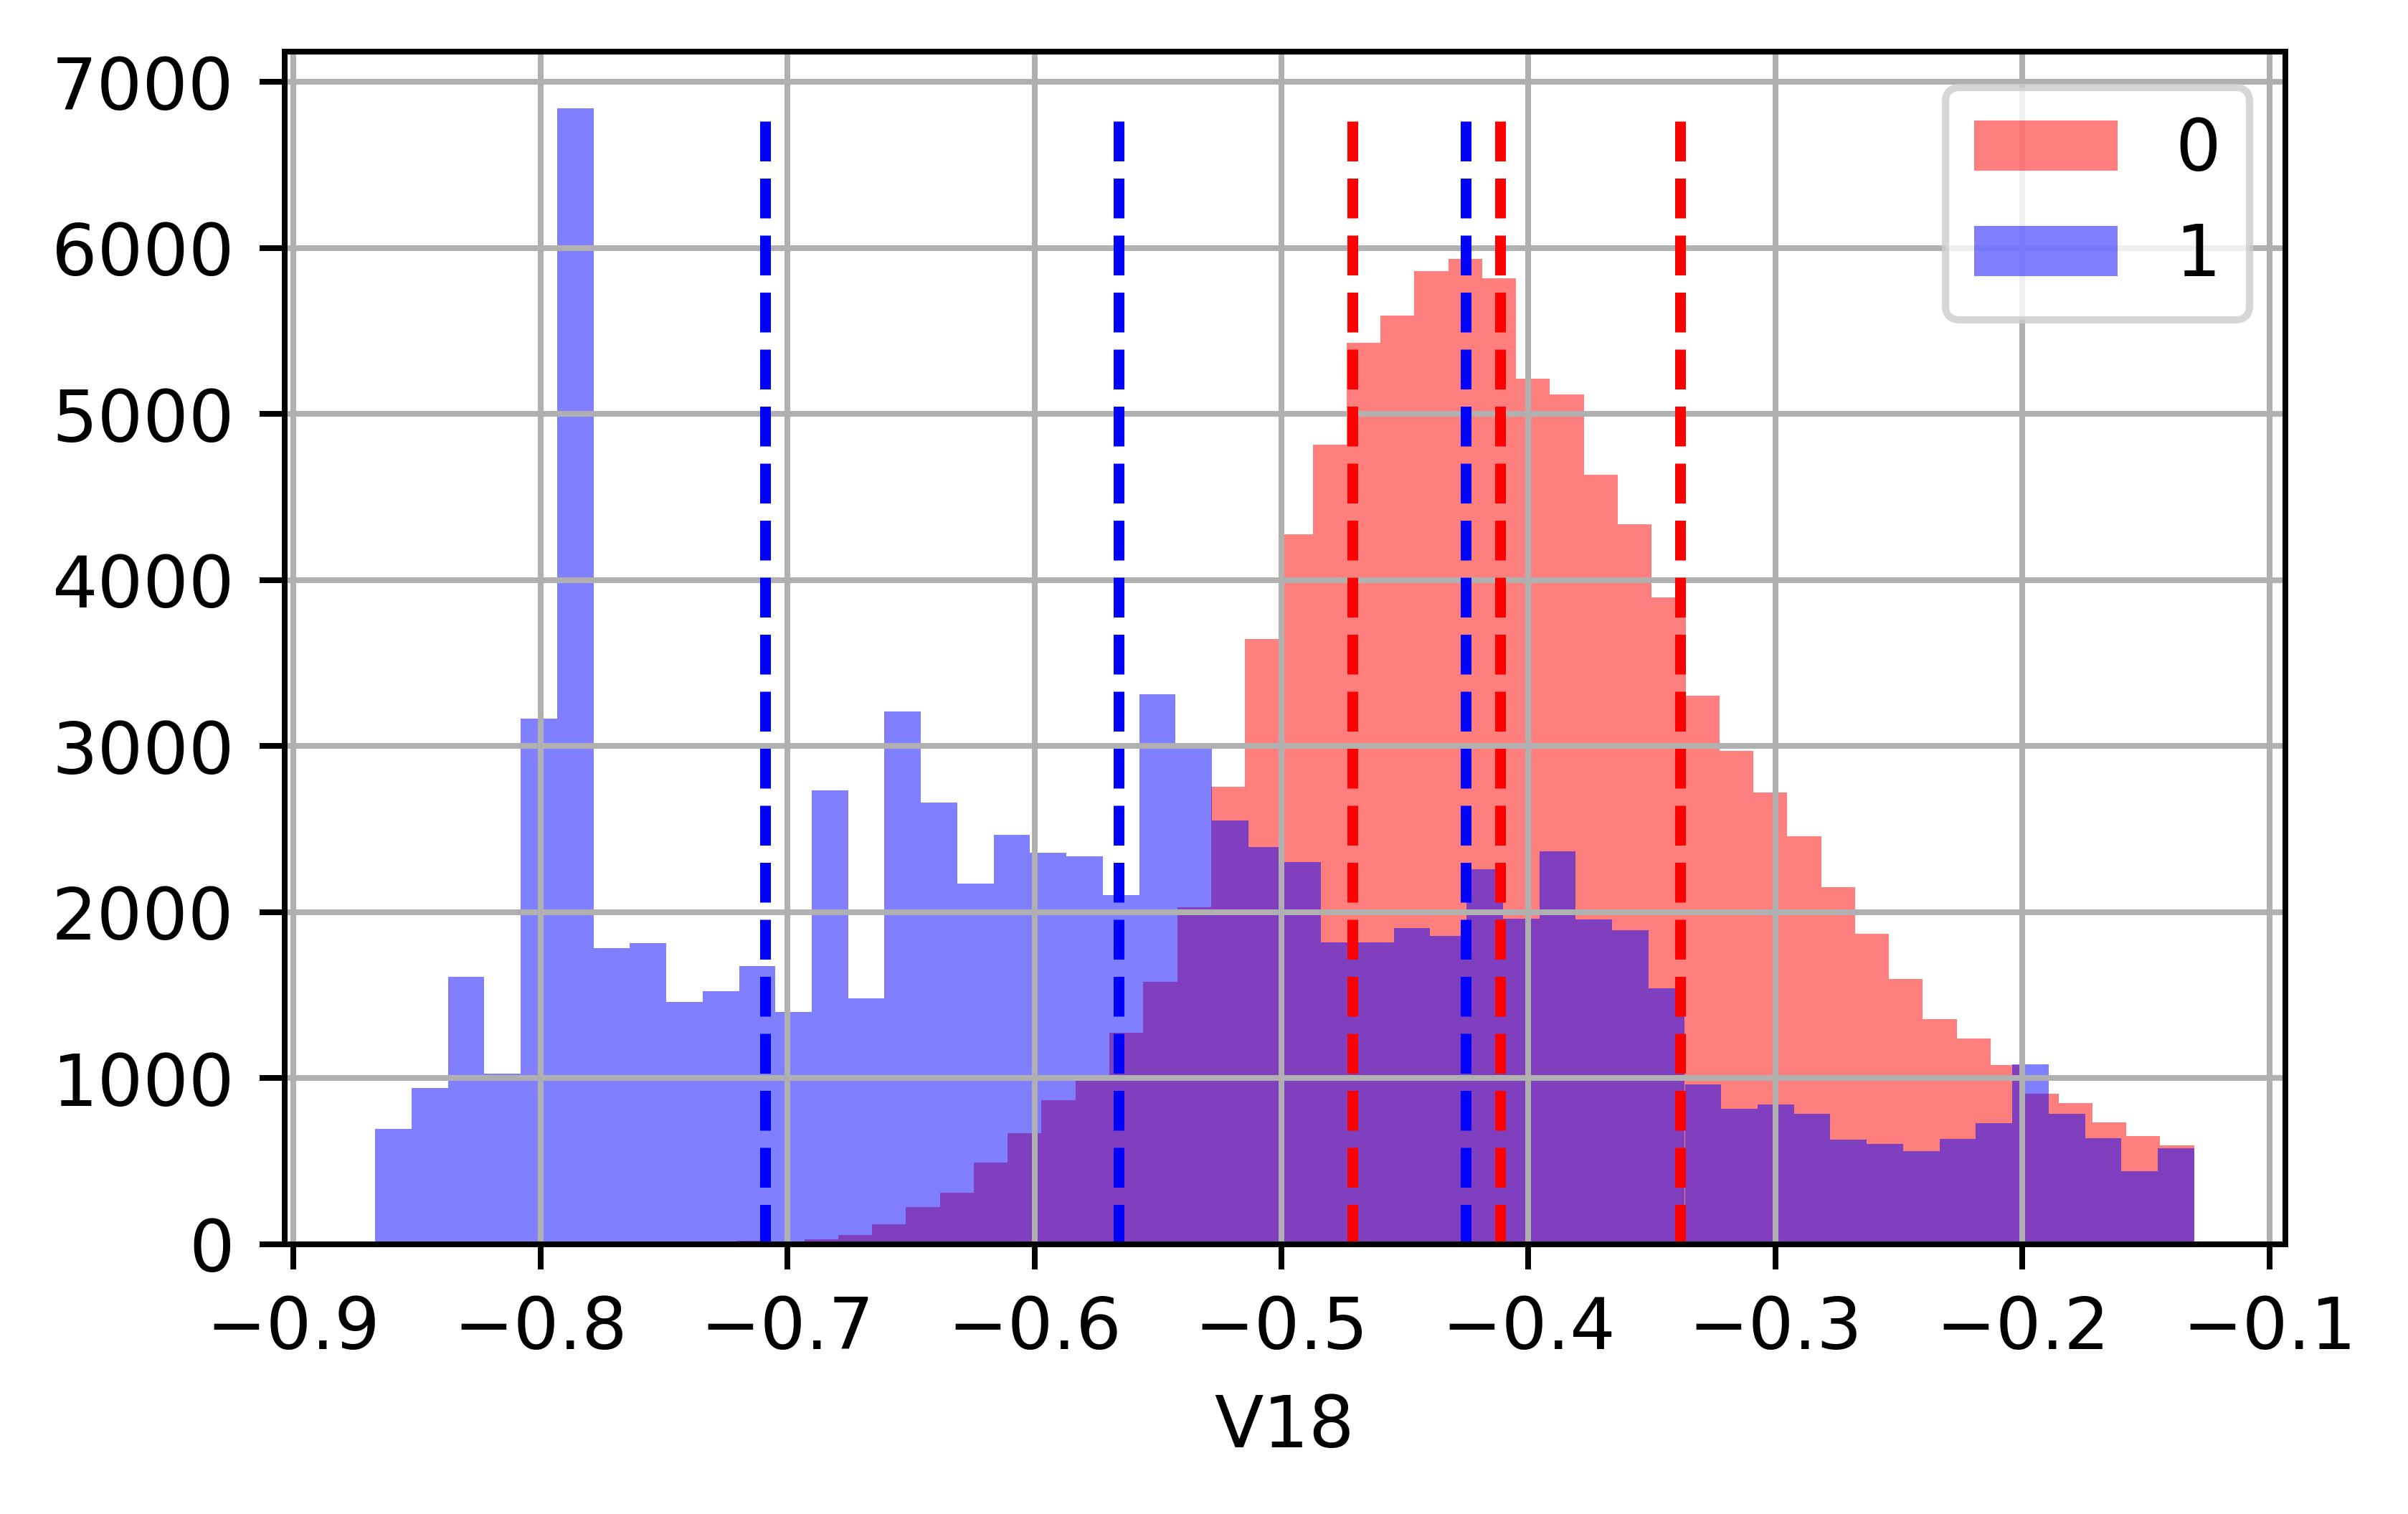
\includegraphics[width=0.18\textwidth]{../code/Task3/Analysis/Hist-V18.jpg}
  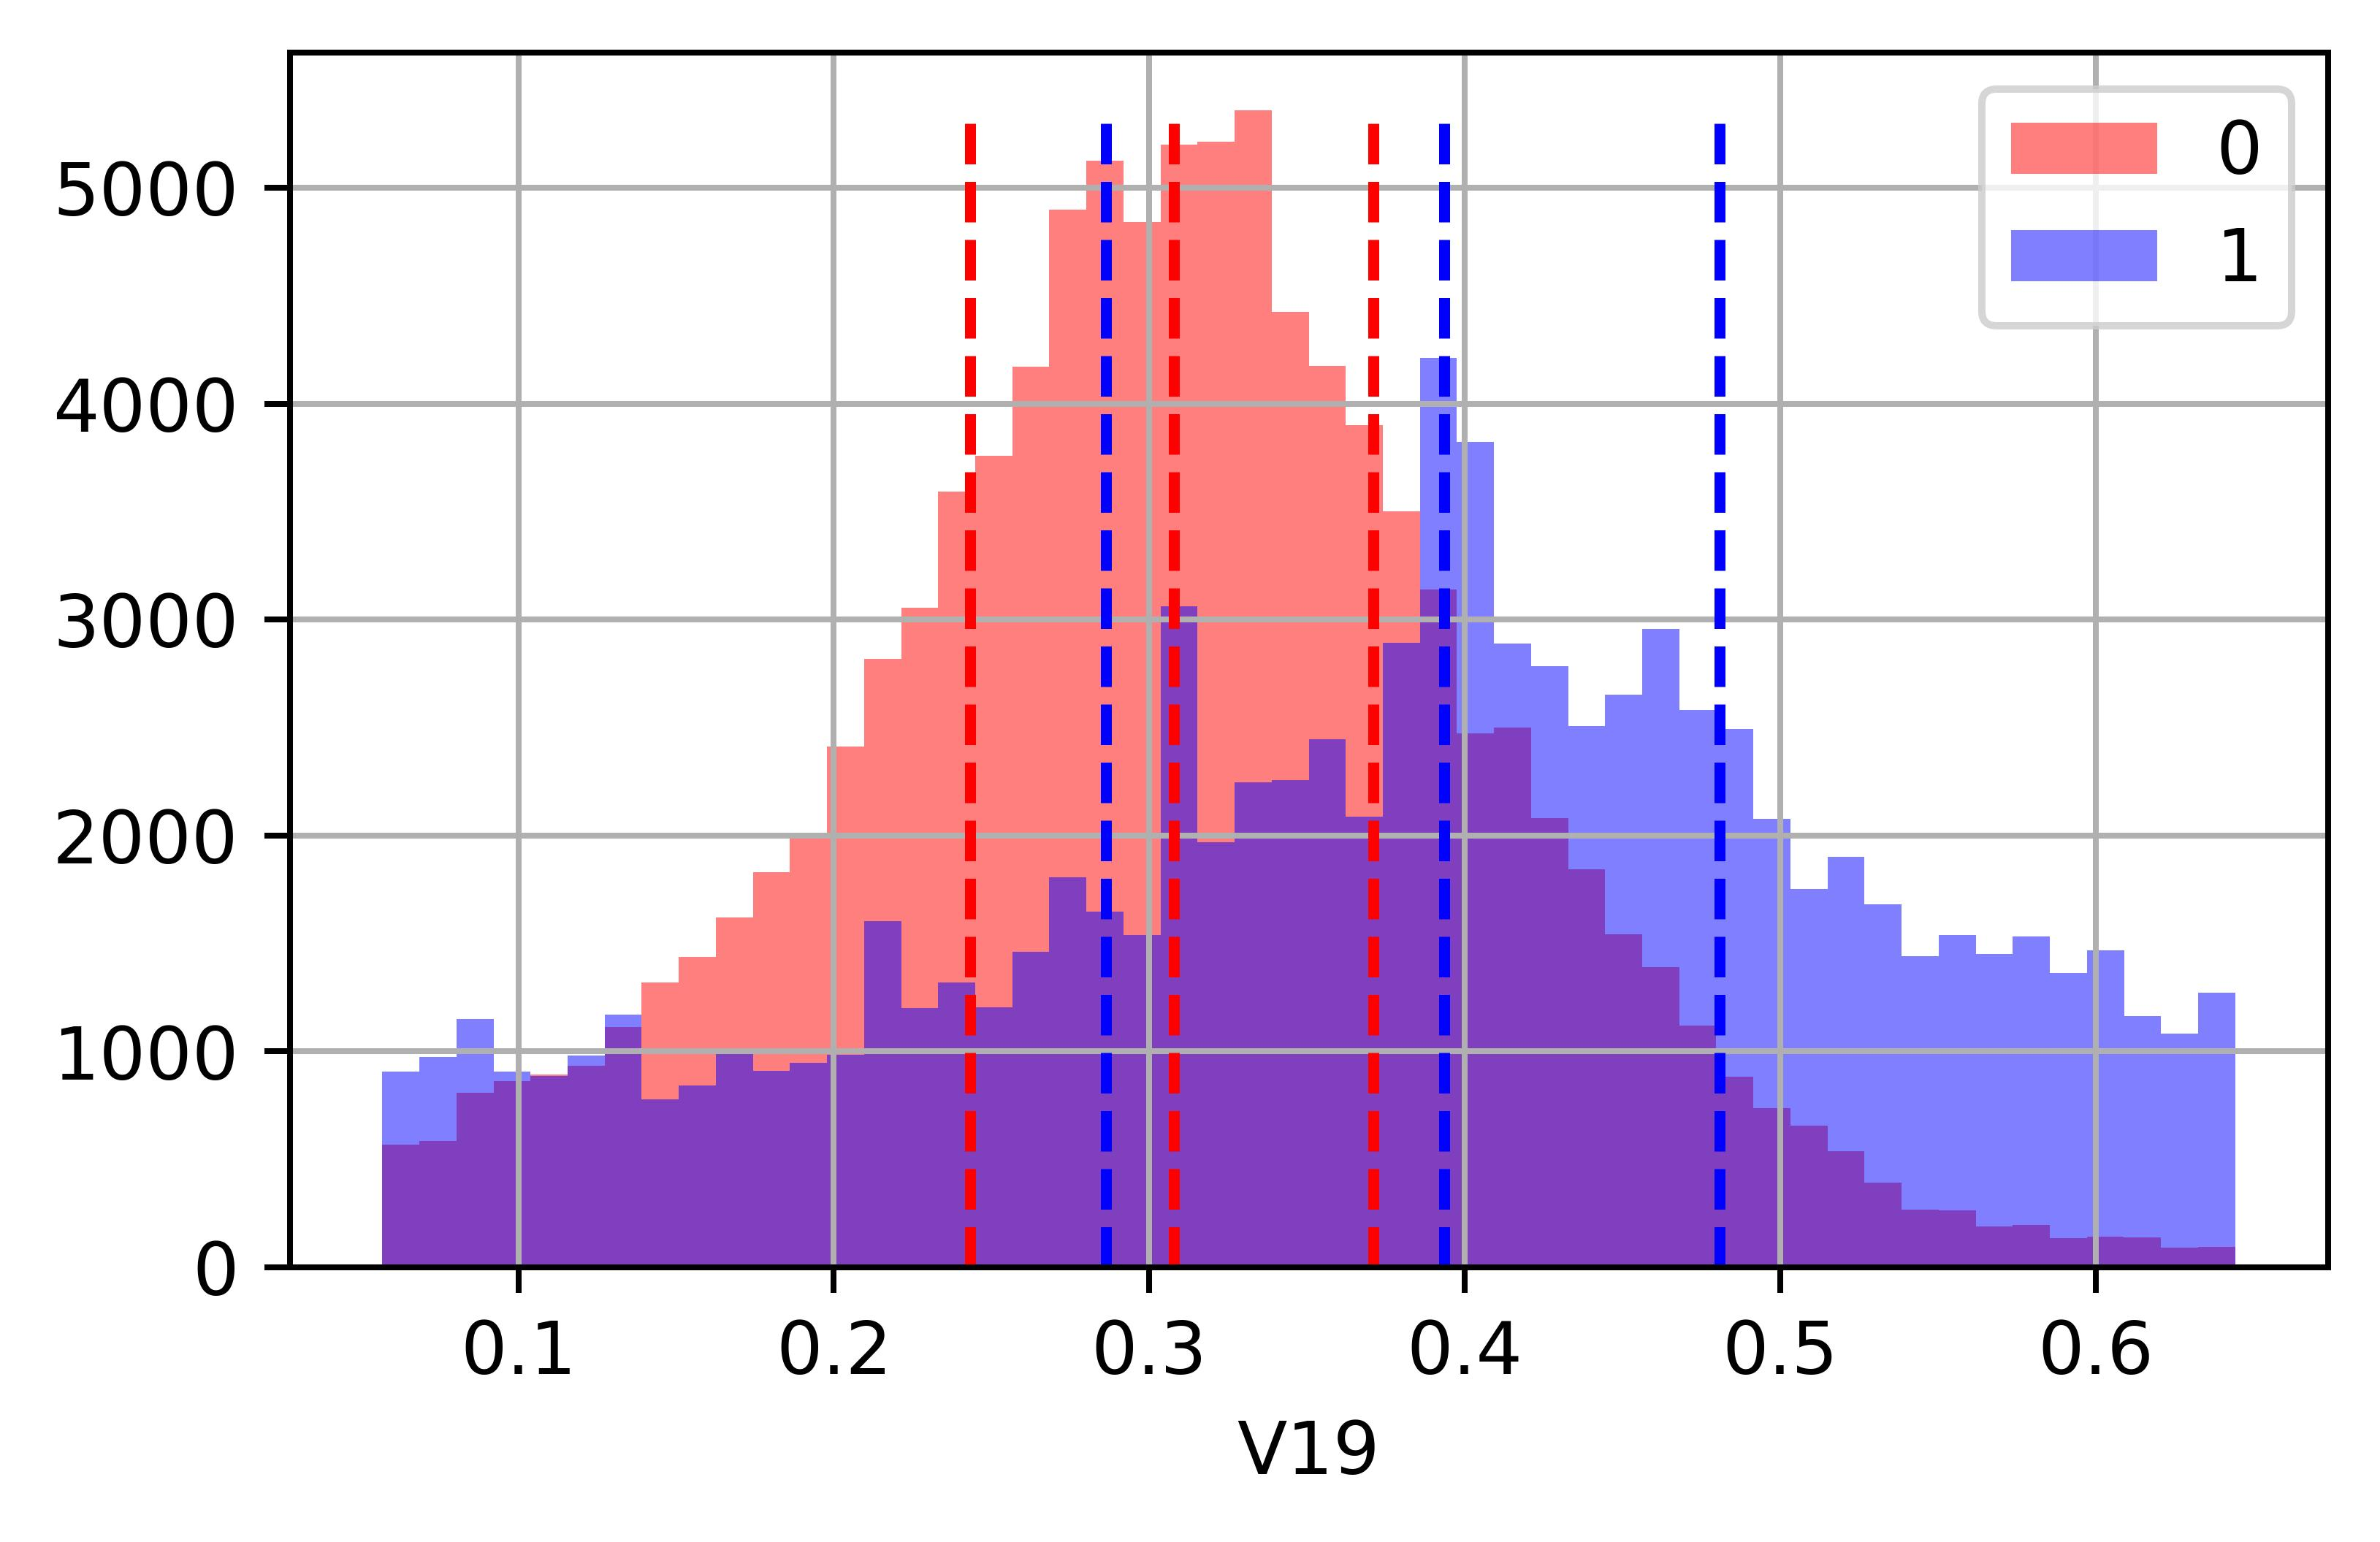
\includegraphics[width=0.18\textwidth]{../code/Task3/Analysis/Hist-V19.jpg}
  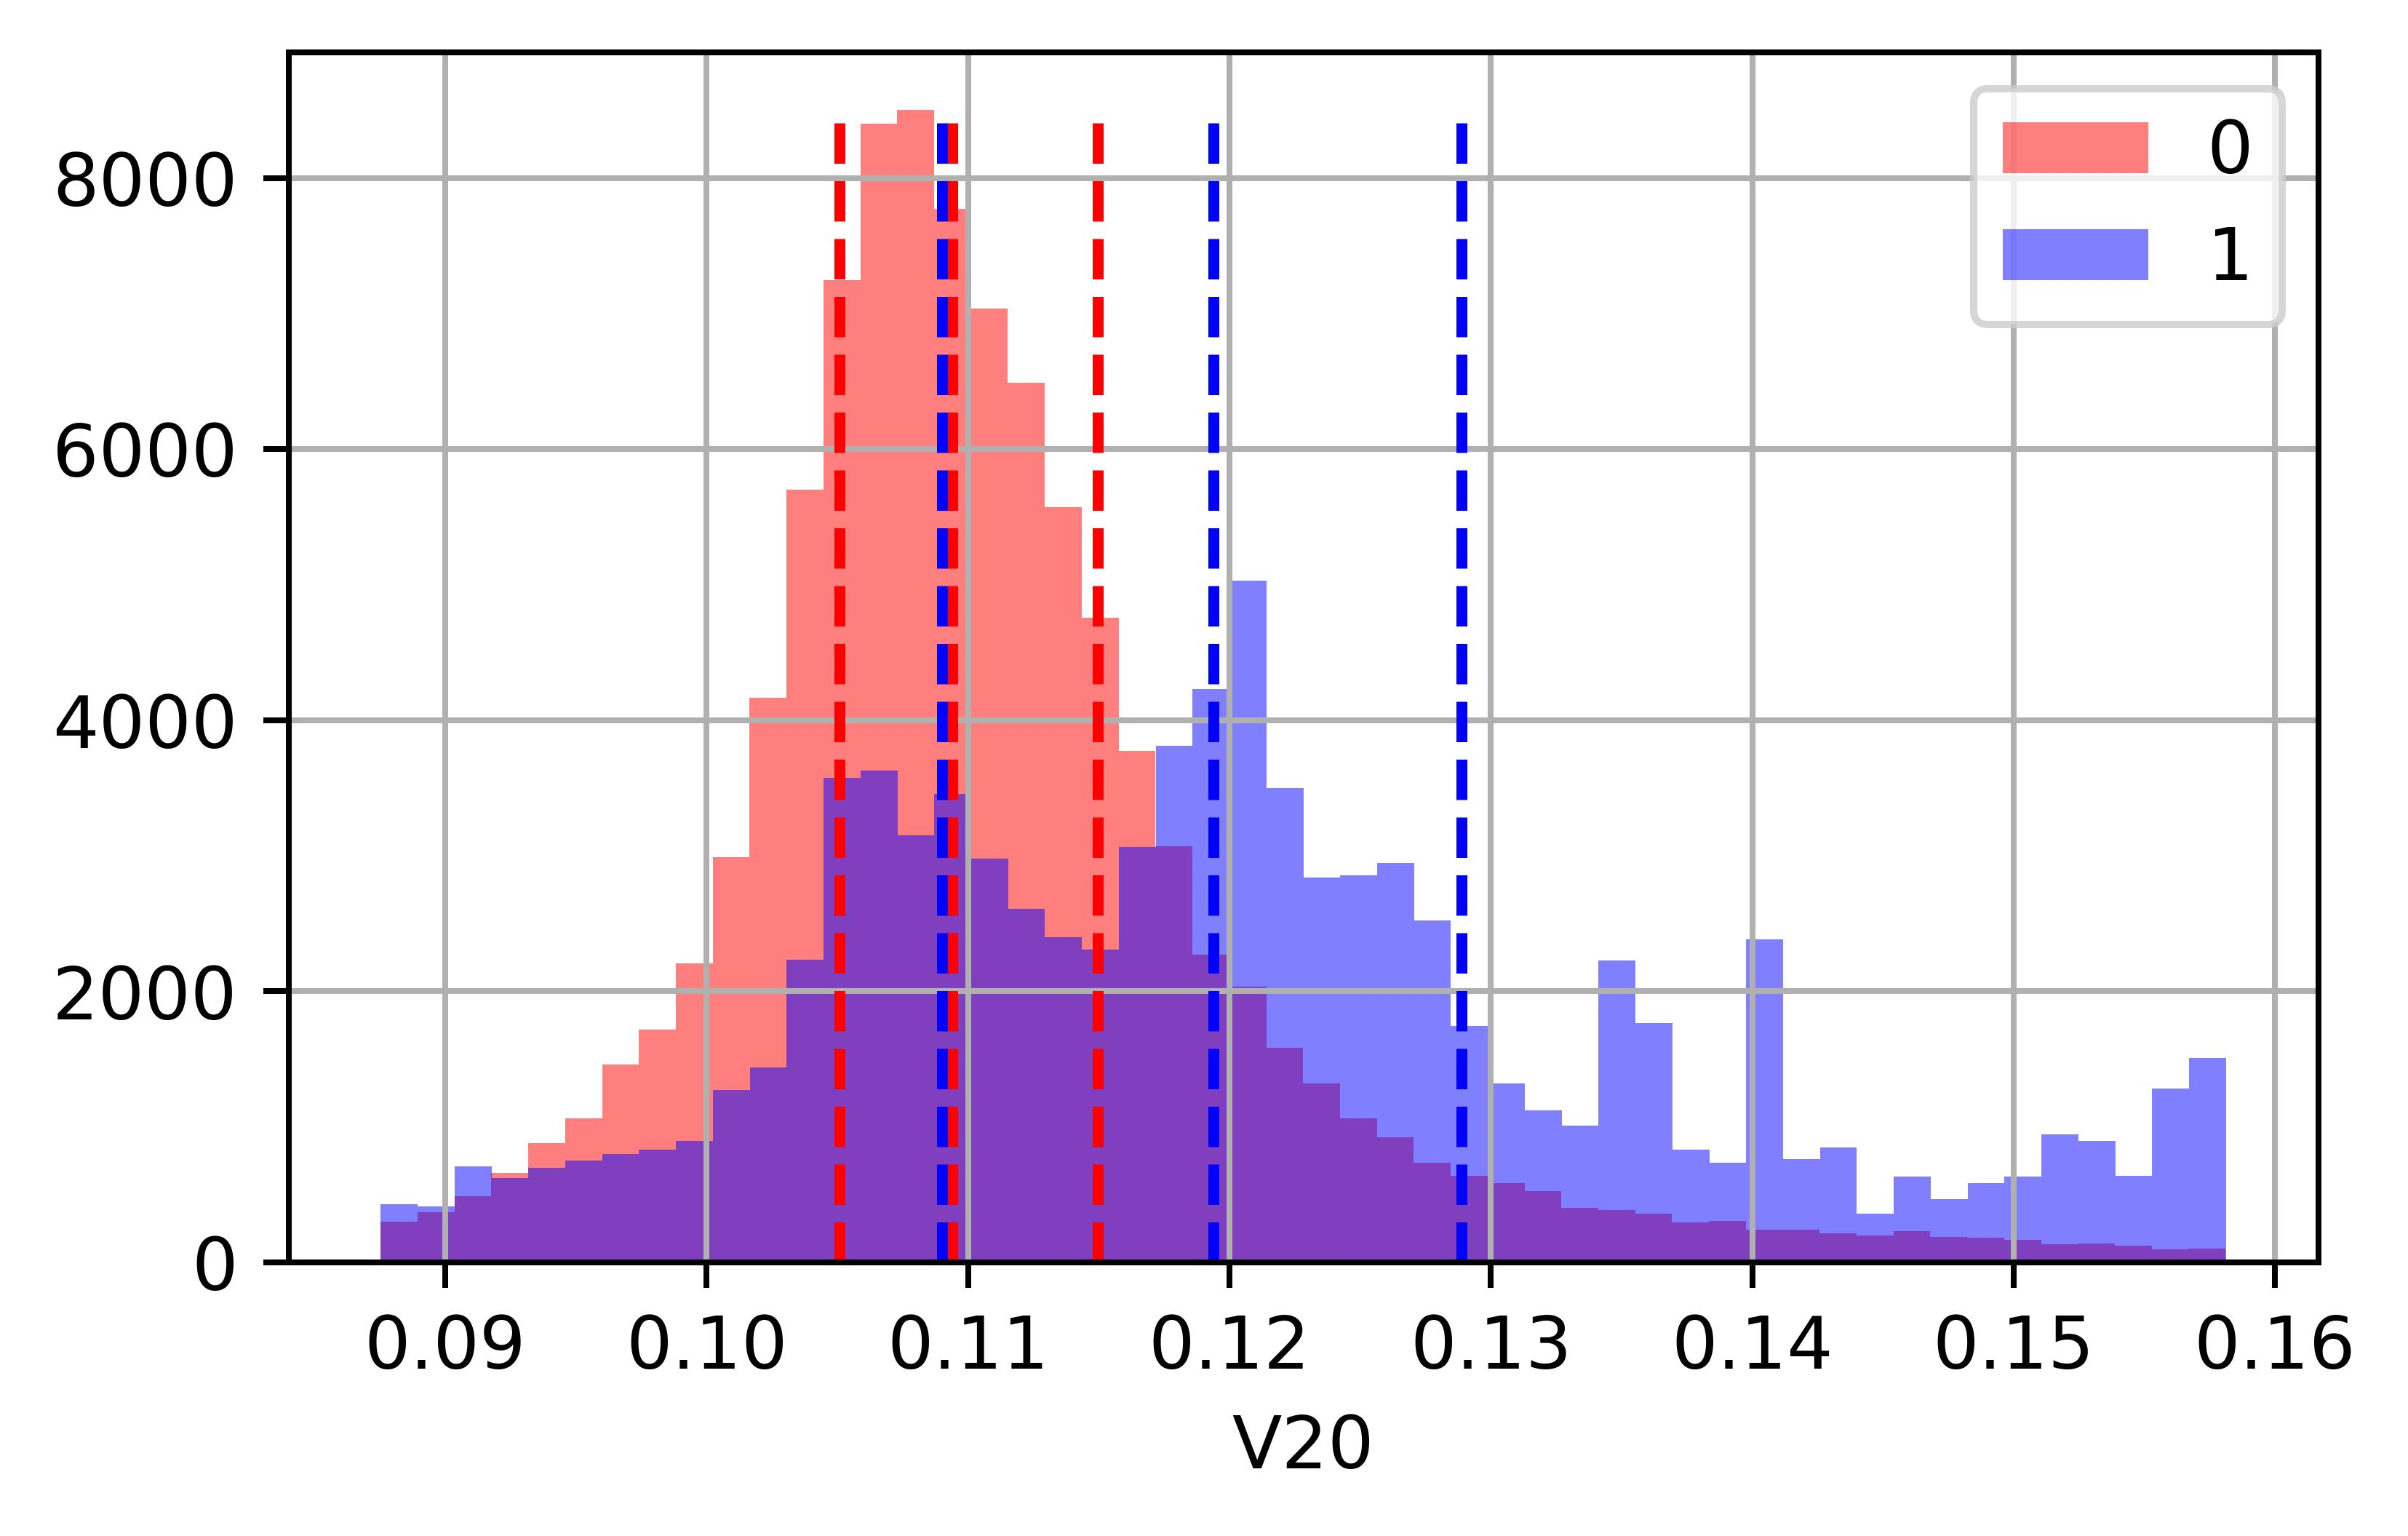
\includegraphics[width=0.18\textwidth]{../code/Task3/Analysis/Hist-V20.jpg} \\
  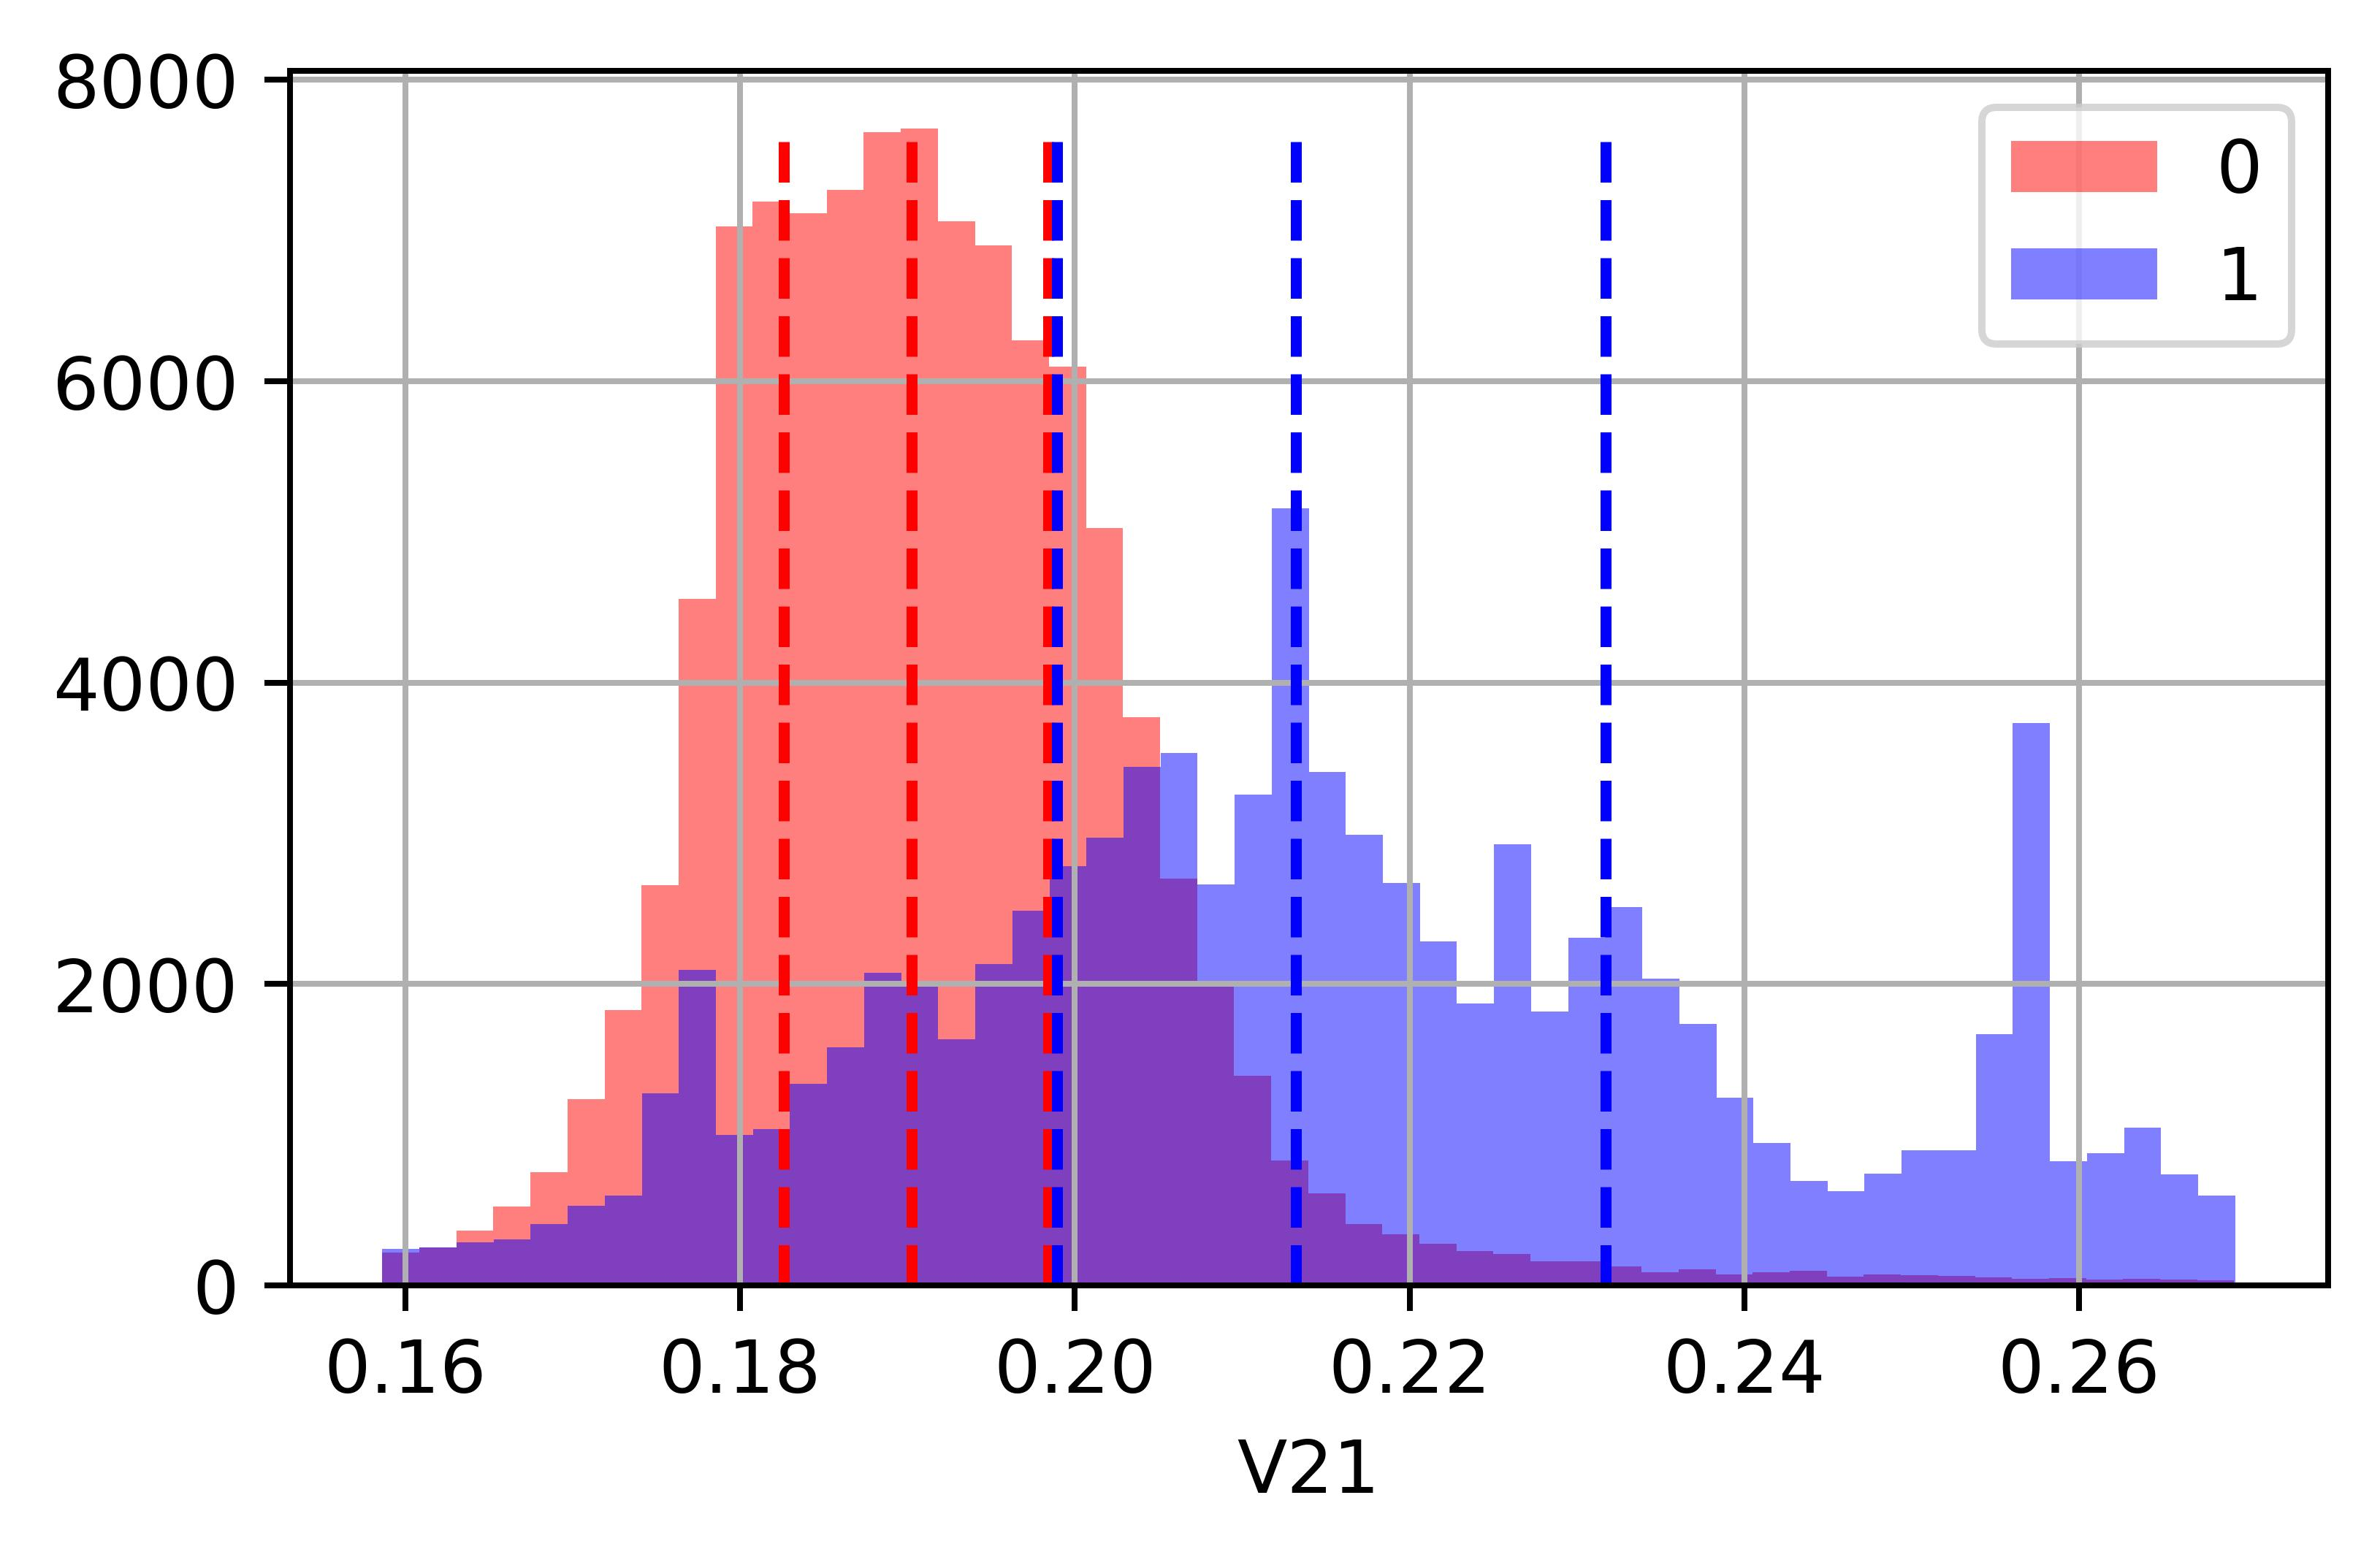
\includegraphics[width=0.18\textwidth]{../code/Task3/Analysis/Hist-V21.jpg}
  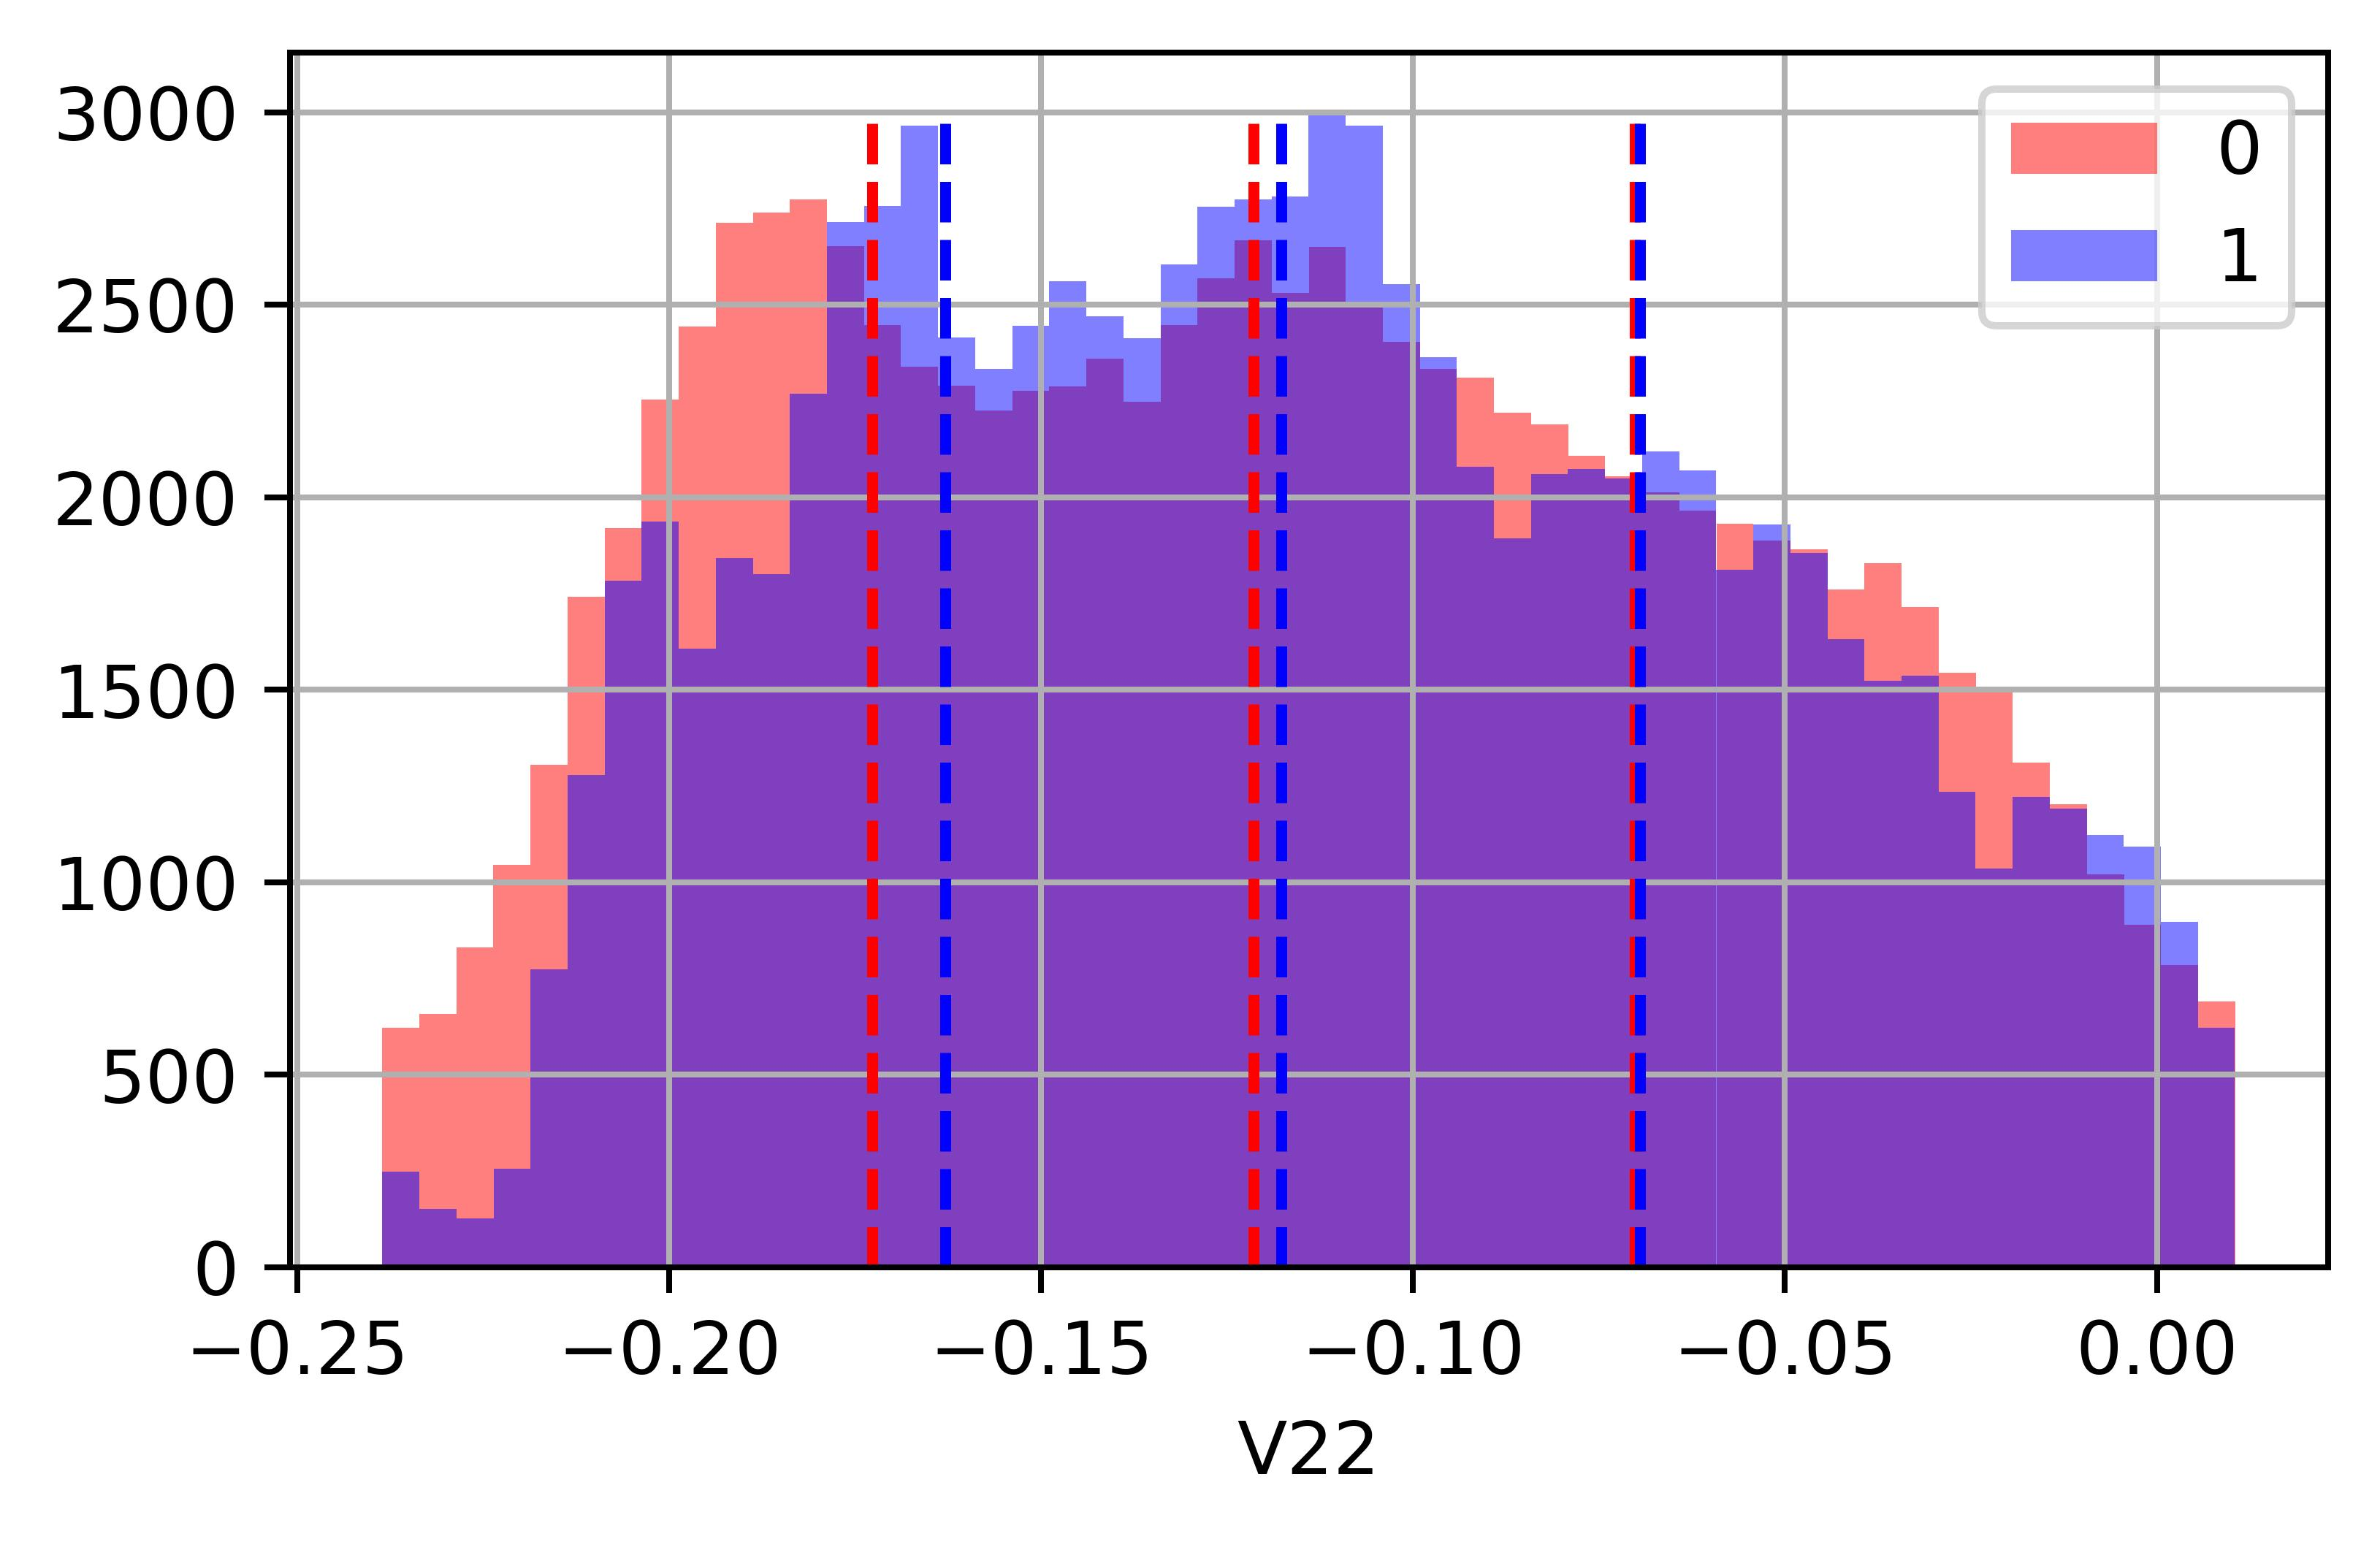
\includegraphics[width=0.18\textwidth]{../code/Task3/Analysis/Hist-V22.jpg}
  \includegraphics[width=0.18\textwidth]{../code/Task3/Analysis/Hist-V23.jpg}
  \includegraphics[width=0.18\textwidth]{../code/Task3/Analysis/Hist-V24.jpg}
  \includegraphics[width=0.18\textwidth]{../code/Task3/Analysis/Hist-V25.jpg} \\
  \includegraphics[width=0.18\textwidth]{../code/Task3/Analysis/Hist-V26.jpg}
  \includegraphics[width=0.18\textwidth]{../code/Task3/Analysis/Hist-V27.jpg}
  \includegraphics[width=0.18\textwidth]{../code/Task3/Analysis/Hist-V28.jpg}
  \includegraphics[width=0.18\textwidth]{../code/Task3/Analysis/Hist-Amount.jpg}
  \caption{The distribution for each feature (the top and bottom $5\%$ points are considered as outliers, and are not shown). The vertical lines shows the position of first, second and third quartiles.}
  \label{task-3-data-distribution-feature}
\end{figure}

\begin{figure}[H]
  \centering
  \includegraphics[width=\textwidth]{../code/Task3/Analysis/corrcoef.jpg} \\
  \caption{Correlation coefficient for each features.}
  \label{task-3-correlation-coefficient}
\end{figure}

After the preparing, the logistic regression and MLP is applied to the data. The Table \ref{task-3-result-1} and Table \ref{task-3-result-2} shows the results of logistic regression and MLP with different hyperparameters. Each test includes $5$ times cross validation ($80\%$ for training set, $20\%$ for training set) and $1$ times that using all data as training set. And the macro f1 score, time and memory cost are recorded.

The result shows that the logistic regression can reach the f1 score higher than $0.95$. Comparing the f1 score given by different raising degree, the results become better as the degree increases, which implies that there exists some potential nonlinearity in the data, but not that significant. On the other hand, the time and memory cost will increase rapidly, which shows that this operator is seem not worth to be done. As for the penalty and feature selection, they will not significantly change the result, which might because that the logistic regression is not prone to overfitting since it is linear and will focus more on the linear separable features.

The MLP model can also reach the f1 score up to $0.95$, and since it highly nonlinear with the ability for capturing increasingly complex patterns hierarchically, there is no need to do the dimension raising. And the feature selection will cause the decreasing of the f1 score also supports this conclusion. On the other hand, The result shows that it will be more sensitive to the hyperparameters, for example, the f1 score will suddenly decreases when the dropout rate changes from $0.1$ to $0.2$.

\begin{table}[H]
  \centering
  \begin{tabular}{|c|c|c|c|c|}
    \hline
    Penalty & \makecell{Dimension                                        \\ Raising \\ (Degree)} & \makecell{Feature \\ Selection} & \makecell{F1 Score \\ (Test/Train)} & \makecell{Time/Mem \\ (s/MB)} \\
    \hline
    None    & None                & False & $0.9586/0.9577$ & $19.5/866$ \\
    \hline
    None    & $2$                 & False & $0.9619/0.9610$ & $33.5/915$ \\
    \hline
    None    & $3$                 & False & $0.9621/0.9612$ & $49.6/973$ \\
    \hline
    Lasso   & None                & False & $0.9579/0.9570$ & $21.5/854$ \\
    \hline
    Ridge   & None                & False & $0.9553/0.9544$ & $19.8/853$ \\
    \hline
    None    & None                & True  & $0.9582/0.9573$ & $16.5/825$ \\
    \hline
  \end{tabular}
  \caption{Preformance for logistic regression. We tested each option with $5$ times cross validation ($80\%$ for training set, $20\%$ for training set) and $1$ times that using all data as training set. The f1 scores showed in the table is the average f1 score for cross validation and using all data as training set (in this case, we just tested the model on training data), the time is the total time for $6$ run, and the memory usage is tested using all the data as training set.}
  \label{task-3-result-1}
\end{table}

\begin{table}[H]
  \centering
  \begin{tabular}{|c|c|c|c|c|}
    \hline
    Dropout & Hidden Size & \makecell{Feature                                \\ Selection} & \makecell{F1 Score \\ (Test/Train)} & \makecell{Time/Mem \\ (s/MB)} \\
    \hline
    $0.1$   & $32$        & False             & $0.9522/0.9548$ & $31.9/929$ \\
    \hline
    $0.2$   & $32$        & False             & $0.9000/0.9207$ & $31.1/916$ \\
    \hline
    $0.1$   & $32$        & True              & $0.9481/0.9480$ & $31.3/899$ \\
    \hline
    $0.1$   & $16$        & False             & $0.9503/0.9493$ & $31.7/929$ \\
    \hline
    $0.1$   & $64$        & True              & $0.9500/0.9501$ & $29.7/902$ \\
    \hline
  \end{tabular}
  \caption{Preformance for MLP. We tested each option with $5$ times cross validation ($80\%$ for training set, $20\%$ for training set) and $1$ times that using all data as training set. The f1 scores showed in the table is the average f1 score for cross validation and using all data as training set (in this case, we just tested the model on training data), the time is the total time for $6$ run, and the memory usage is tested using all the data as training set.}
  \label{task-3-result-2}
\end{table}

\section{Summary}

During this project, we solved three classification tasks: student placement prediction, feature-based multi-class classification, and fraud detection. For each task, we followed a structured data analytical process, including data exploration, feature engineering, model implementation and performance evaluation.

Different kind of machine learning methods and data analysis techniques are used. In the data exploration part, the correlation coefficient is employed to analyze the relationships between features and label, then the visualization techniques such as parallel coordinate plots and histogram are used for a more intuitive result. With these we figure out the importance of features and the distribution of data.

In the feature engineering, we applied the $k$ nearest neighbors imputer to fill in the missing values and enhance the data through feature selection and dimension raising. And for modeling and prediction, we implemented all the key details of logistic regression, decision tree and MLP by PyTorch, instead of simply invoking the black-box algorithms, and ensured the repeatable results. Additionally, we fully recorded the model training process, including the time and memory cost, and try to do some optimization on them by learning rate adjustment and parallel computing.

\subsection{Discovery \& insights}

For task 1, the manually designed features combination and correlation analysis can help imrpove the logistic regression on predominantly linear data, though dimension raising offered limited improvement. For task 2, the $k$ nearest neighbors imputer improved data integrity by filling the missing values, and MLP excelled at capturing nonlinear relationships, with feature selection providing minimal benefit. As for task 3, feature selection based on correlation coefficients with dimension raising can lead to a higher performance for both logistic regression and MLP, though higher-degree raising incurred excessive computational costs.

All the three task shows the importance of feature engineering and model selection. The linear models like logistic regression preforms a better reliability and efficiency especially on linearly separable data like tasks 1 and 3, while nonlinear models like MLP can reach a better performance in the complex multi-class problem such as task 2. On the other hand, the effectiveness of feature engineering varies by task, which needs adjustments based on the data. Moreover, performance optimization involves balancing between the accuracy and computational cost, which is shown in task 3 that the dimension raising will significantly increase the time and memory consumption.

In terms of hyperparameter tuning, applying regularization (e.g., lasso or ridge for logistic regression, maximun depth for decision tree, dropout for MLP) can help reduce the influence of noise and outliers, which prevent the model from overfitting and ensuring the generalization in the meanwhile. Further more, the parallel computing as we implemented in decision tree and MLP can significantly accelerate the training, but must be balanced against memory constraints and convergence stability.

\subsection{Future work}

In data preparing, on possible way to optimize the model performance is to employ automated feature engineering tools insteal of manual design, which can improve feature selection and generation. As for decision tree, ensemble methods (e.g., random forests or gradient boosting trees) may help deal with the overfitting of decision tree. Further more, one important application is to process the data stream instantly, i.e., adapt the models to a dynamic environment and input. Especially for the fraud detection, an earlier detection may lead to a less loss. One way to speed up the training and predicti is the distributed computing frameworks, which can also help training with the large-scale datasets.

\newpage

\bibliographystyle{unsrt}
\bibliography{reference.bib}
\addcontentsline{toc}{section}{References}

\newpage

\appendix
\renewcommand\thesection{\Alph{section}}

\section{Author Contributions}

\begin{table}[H]
  \centering
  \begin{tabular}{|c|c|c|}
    \hline
    Name & \makecell{Percentage of \\ contributions} & Details \\
    \hline
    \makecell{WANG Zeyu            \\ 24056788G}   &        $34\%$                 & Implement logistic regression and task 3. Write report\\
    \hline
    \makecell{YANG Xirui           \\ 24135668G}  &               $33\%$          &Implement MLP and task 1. Write report \\
    \hline
    \makecell{Wu Tianxiao          \\ 24084591G} &                      $33\%$   & Implement decision tree and task 2. Write report\\
    \hline
  \end{tabular}
  \caption{Contributions.}
\end{table}

\end{document}